% siminos/reversal/LC21.tex      pdflatex LC21; bibtex LC21
% $Author: predrag $ $Date: 2021-12-24 01:25:20 -0500 (Fri, 24 Dec 2021) $

% Title:    "A chaotic lattice field theory in one dimension"
% Authors:  Han Liang and Predrag Cvitanovi{\'c}
% web, BibTex name:      LC21.pdf  \cite{LC21}

%%%%%%%%%%%%%%%%%%%%%%%%%%%%%%%%%%%%%%%%%%%%%%%%%%%%%%%%%%%%%%%%%%%%%%%
             \newif\ifboyscout\boyscouttrue          %% comments     %%
             \newif\ifsubmission\submissionfalse     %% internal     %%
             \newif\ifblog\blogfalse %% section shared with blogCats %%
%%%%% Toggle between draft and public versions:  %%%%%%%%%%%%%%%%%%%%%%
% \boyscoutfalse                         % public, hyperlinked       %%
% \boyscoutfalse\submissiontrue          % for J Phys A              %%
%%%%%%%%%%%%%%%%%%%%%%%%%%%%%%%%%%%%%%%%%%%%%%%%%%%%%%%%%%%%%%%%%%%%%%%

% arXiv-v1/ commit                                      2019-11-0?
% jphysa-v1/ submission #??????                         2019-1?-0?

% Predrag   LC21 version 2.0            2021-12-15
% Predrag   LC21 version 1.1            2021-08-12
% title was      {Time reversal for discrete time dynamical systems}
% Predrag   LC21 version 0.1            2021-05-15
%           started with CL18 kittens/*.tex
% Predrag   CL18 version 1.0            2020-09-19
% Predrag   CL18 version 0.1            2019-08-15
% Predrag   GHJSC16 draft               2017-09-26

\documentclass[12pt]{iopart}
% loads AMS amsgen, amsfonts, amsbsy, amssymb:
\usepackage{iopams} % to load AMS extension fonts msam and msbm
                     % the blackboard bold alphabet, extra maths symbols
                     % and extra definitions for bold Greek letters.
                     % do not use amsmath.sty

\pdfminorversion=4  % the very start the TeX file, so PDF or bitmap figures
                    % are PDF version 1.4 or lower


% \usepackage{mathtools} % to do {cases}, conflicts
\usepackage[pdftex]{graphicx}
\graphicspath{{../figs/}{../Fig/}}  %% directories with graphics files
% for submission, copy figures into /jphysa-v1/ rename them, then
% comment out the \graphicspath{

\ifsubmission
\else % prepare hyperlinked
    \usepackage{color} % dvips allows for colors
    \usepackage[colorlinks]{hyperref} %% hyperlinks
\fi

%\hypersetup{
%   pdfauthor=Space is the Place Collective,
%   pdfkeywords=spatiotemporal,
%   pdftitle=herding cats
%            }

    \ifsubmission\else
\input{biblatex}    % this makes references hyperlinked
\addbibresource{../bibtex/siminos.bib}
    \fi
% siminos/reversal/defsReversal.tex
% $Author: predrag $ $Date: 2021-12-12 22:57:47 -0500 (Sun, 12 Dec 2021) $

% started with % siminos/kittens/defsKittens.tex

%%%%%%%%%%%%%% CL18 specific %%%%%%%%%%%%%%%%%%%%%%%%%%%%
\newcommand{\fundPip}{fundamental parallelepiped}
\newcommand{\FundPip}{Fundamental parallelepiped}

\newcommand{\SLn}[2]{\ensuremath{\textrm{SL}_{#1}(#2)}}
\newcommand{\class}[1]{\ensuremath{{\cal C}_{#1}}}
\newcommand{\PP}{P}    % projection operator,          Predrag  2019-10-16
\newcommand{\lattice}{\ensuremath{\mathcal{L}}}
    % PC 2021-08-05: from https://tex.stackexchange.com/questions/86569/creating-uniformly-sized-boxes-around-text
\newcommand{\sitebox}[1]{%
        {% open a group for a local setting
   \setlength{\fboxsep}{-2\fboxrule}% the rule will be inside the box boundary
   \fbox{\hspace{1.2pt}\strut$#1$\hspace{1.2pt}}% print the box, with some padding at the left and right
        }% close the group
                        } %%%%%%%%%%%%%%%%%%%%%%%%%%%%%


%%%%%% Referencing equations etc, Nonlinearity style only %%%%%%%
\newcommand{\conf}{\ensuremath{x}} %Configuration space coordinate
\newcommand{\Fu}{\tilde{u}}
\newcommand{\twot}{periodic orbit} %Predrag experiment 2020-03-18
\newcommand{\twots}{periodic orbits}
\newcommand{\twoT}{Periodic orbit}
\newcommand{\twoTs}{Periodic orbits}
%\newcommand{\twot}{invariant 2-torus}
%\newcommand{\twots}{invariant 2-tori}
%\newcommand{\twoT}{Invariant 2-torus}
%\newcommand{\twoTs}{Invariant 2-tori}
\newcommand{\dtor}{invariant $d$-torus} % Predrag, to distinguish from a PO
\newcommand{\dtors}{invariant $d$-tori}
\newcommand{\dTor}{Invariant $d$-torus}
\newcommand{\dTors}{Invariant $d$-tori}
\newcommand{\lattstate}{lattice state}
\newcommand{\Lattstate}{Lattice state}
\newcommand{\orbit}{orbit} % Predrag 2021-08-10: retired ChaosBook {prime cycle}
\newcommand{\Orbit}{Orbit}
\newcommand{\templatt}{temporal cat}     % Predrag, experimental
\newcommand{\tempLatt}{Temporal cat}     % Predrag, experimental
\newcommand{\spt}{spatiotemporal}
\newcommand{\Spt}{Spatiotemporal}
\newcommand{\catlatt}{spatiotemporal cat}     % Predrag, experimental
\newcommand{\catLatt}{Spatiotemporal cat}     % Predrag, experimental
\newcommand{\Henon}{H\'enon}
\newcommand{\HenonMap}{H\'enon map}
\newcommand{\henlatt}{temporal H{\'e}non}     % Predrag, experimental
\newcommand{\Henlatt}{Temporal H{\'e}non}     % Predrag, experimental
\newcommand{\henSTlatt}{{\spt} H{\'e}non}     % Predrag, experimental
\newcommand{\HenSTlatt}{{\Spt} H{\'e}non}     % Predrag, experimental
\newcommand{\bcs}{bc's}
\newcommand{\PV}{Percival-Vivaldi}
\newcommand{\AW}{Adler-Weiss}
\newcommand{\GO}{Gutkin-Osipov}
\newcommand{\sPe}{screened Poisson equation}
\newcommand{\SPe}{Screened Poisson equation}
\newcommand{\zetatop}{\ensuremath{1/\zeta_{\mbox{\footnotesize top}} }}
\newcommand{\msr}{\ensuremath{\rho}}                % measure
%\newcommand{\Msr}{{f(}}                 % Boris frequency AKA measure
\newcommand{\Msr}{{\mu}}                % Predrag, experimental: measure
\newcommand{\dMsr}{{d\mu}}              % measure infinitesimal
\newcommand{\SRB}{{\rho_0}}             % natural measure
\newcommand{\coord}{q}        % configuration space q coordinate, dual to p
\newcommand{\jMps}{\ensuremath{J}}   % jacobian matrix, phase space/state space
% \newcommand{\jMps}{\ensuremath{{\bf J}}}  % bold fundamental matrix phase space
\newcommand{\monodromy}{\ensuremath{M}}   % monodromy matrix, full Poincare cut
\newcommand{\jMorb}{{\ensuremath{\mathcal{\jMps}}}}
\newcommand{\jMat}{\mathbb{\jMps}}

%\newcommand{\ssp}{\ensuremath{x}}               % state space point
\newcommand{\ssp}{\ensuremath{\phi}}             % kittens lattice site field
\newcommand{\cssp}{\ensuremath{\tilde{\phi}}}    % Complex state space point
\newcommand{\source}{{J}}
\newcommand{\sourceFT}{{\tilde{J}}}
\newcommand{\derSource}{\frac{d~}{d\source}}
\newcommand{\derSourceFT}{\frac{d~}{d\sourceFT}}


%%%%%% Boris definitions
\newcommand{\Mm}{\ensuremath{\mathsf{M}}}
%\newcommand{\Xx}{\ensuremath{\mathsf{X}}}      % Boris
\newcommand{\Xx}{\ensuremath{\mathsf{\Phi}}}      % kittens lattice field
\newcommand{\xx}{\ensuremath{\mathsf{\boldsymbol{\phi}}}} %{\bphi}}}      % kittens lattice field
\newcommand{\Aa}{\ensuremath{\bar{\A}}}
\newcommand{\A}{\ensuremath{\mathcal{A}}}       % alphabet
\newcommand{\Ai}{\ensuremath{\mathcal{A}_0}}    % alphabet interior (was inner)
\newcommand{\Ae}{\ensuremath{\mathcal{A}_1}}    % alphabet exterior (was outer)
\newcommand{\B}{\mathcal{B}}
\newcommand{\D}{\mathcal{D}}
\newcommand{\R}{\ensuremath{\mathcal{R}}}
\newcommand{\Pol}{\mathcal{P}}                  % Boris
\newcommand{\gd}{\mathsf{g}}
% Dirichlet Green's function
\newcommand{\gp}{\mathsf{g}^0}
% Periodic Green's function
%\newcommand{\m}{\ensuremath{\mathsf{m}}}     % Boris
\newcommand{\m}{\ensuremath{m}}     % Predrag experimental 2016-11-08
%\newcommand{\q}{\ensuremath{\mathsf{m}}}     % Boris
\newcommand{\q}{\ensuremath{q}}     % Predrag experimental 2016-11-08
\newcommand{\reals}{\mathbb{R}}
\newcommand{\naturals}{\mathbb{N}}
\newcommand{\integers}{\ensuremath{\mathbb{Z}}}
\newcommand{\Zz}{\ensuremath{\mathbb{Z}^2}}
%\newcommand{\Det}{\mbox{\rm Det}\,}
%\newcommand{\ZNT}{\mathbb{Z}^2_{\mbox{\scriptscriptstyle{NT}}}}
\newcommand{\ZLT}{\mathbb{Z}^2_{\scriptscriptstyle\mathrm{LT}}}
\newcommand{\MmR}{\Mm_\R}
\newcommand{\length}{\mathcal{D}}
\newcommand{\deltaX}{\ensuremath{{\delta x}}}       %trajectory displacement
%! Undefined control sequence.
%   \example
\newcommand{\pde}{\partial}
\newcommand{\vel}{\ensuremath{v}}   % state space velocity
\newcommand{\Idg}{\ensuremath{\mathbf{1}}}
\newcommand{\Cn}[1]{\ensuremath{\textrm{C}_{#1}}}
\newcommand{\jacobianOrb}{orbit Jacobian matrix}
\newcommand{\JacobianOrb}{Orbit Jacobian matrix}
\newcommand{\jacobianOrbs}{orbit Jacobian matrices}
\newcommand{\JacobianOrbs}{Orbit Jacobian matrices}
\newcommand{\HillDet}{Hill determinant}
\newcommand{\ecs}{exact coherent structure}
\newcommand{\Ecs}{Exact coherent structure}
%%%%%%%%%%%%%%%%%%%%%%%%%%%%%%%%%%%%%%%%%%%%%%%%%%%%%%%%%%%%%%%%%

\newcommand{\NBBpost}[2]{\item[#1 Burak] {#2}}
\newcommand{\PCpost}[2]{\item[#1 Predrag] {#2}}
\newcommand{\BGpost}[2]{\item[#1 Boris] {#2}}
\newcommand{\AKSpost}[2]{\item[#1 Adrien] {#2}}
\newcommand{\RJpost}[2]{\item[#1 Rana] {#2}}
\newcommand{\LHpost}[2]{\item[#1 Li Han] {#2}}
\newcommand{\MNGpost}[2]{\item[#1 Matt] {#2}}
\newcommand{\XDpost}[2]{\item[#1 Xiong] {#2}}
\newcommand{\HLpost}[2]{\item[#1 Han] {#2}}

\ifboyscout %%%%%%%% DISPLAY COMMENTS IN THE TEXT %%%%%%%%%%%%%%%%%%%%
            %%%%%%%% turn on labeling of equations on margins %%%%%%%%
    % also search the text for lines starting with %%  to
    % locate various internal comments, recent edits etc.
    \typeout{============ COMMENTED =====}
  \newcommand{\PublicPrivate}[2]
    {\marginpar{\color{blue}$\Downarrow$\footnotesize PRIVATE}%
    {\color{blue}#2}%
    \marginpar{\color{blue}$\Uparrow$\footnotesize PRIVATE}}
  \newcommand{\PC}[2]% {$\footnotemark\footnotetext{Predrag #1: #2}$}
                     {\begin{quote}\PCedit{[#1 Predrag] \small #2}\end{quote}}
  \newcommand{\PCedit}[1]{{\color{magenta}#1}}
  \newcommand{\HL}[2]%{$\footnotemark\footnotetext{Han: #1}$}
                     {\begin{quote}\HLedit{[#1 Han] \small #2}\end{quote}}
  \newcommand{\HLedit}[1]{{\color{blue}#1}}
  \newcommand{\BG}[2]% {$\footnotemark\footnotetext{Boris #1: #2}$}
                     {\begin{quote}\BGedit{[#1 Boris] \small #2}\end{quote}}
  \newcommand{\BGedit}[1]{{\color{red}#1}}
  \newcommand{\AKS}[2]{$\footnotemark\footnotetext{Adrien #1: #2}$}
  \newcommand{\AKSedit}[1]{{\color{green}#1}}
  \newcommand{\RJ}[2]%{$\footnotemark\footnotetext{Rana #1: #2}$}
                     {\begin{quote}\RJedit{[#1 Rana] \small #2}\end{quote}}
  \newcommand{\RJedit}[1]{{\color{green}#1}}
  \newcommand{\MNG}[2]{$\footnotemark\footnotetext{Matt #1: #2}$}
  \newcommand{\MNGedit}[1]{{\color{red}#1}}
  \newcommand{\LH}[2]%{$\footnotemark\footnotetext{Rana #1: #2}$}
                     {\begin{quote}\LHedit{[#1 Li] \small #2}\end{quote}}
  \newcommand{\LHedit}[1]{{\color{green}#1}}
  \newcommand{\Private}[1]{{\color{blue}#1}}
  \newcommand{\toCB}{\marginpar{\footnotesize 2CB}}  % to compare with ChaosBook
  \newcommand{\inCB}{\marginpar{\footnotesize now in CB}} % entered in ChaosBook
  \newcommand{\CBlibrary}[1]
             {\href{http://ChaosBook.org/library/#1.pdf} { (click here)}}
\else % drop comments
      % do not turn on labeling of equations on margins
  \typeout{============ UNCOMMENTED =====}
  \newcommand{\PublicPrivate}[2]{#1}
  \newcommand{\PC}[2]{}{}
  \newcommand{\PCedit}[1]{#1}
  \newcommand{\HL}[2]{}
  \newcommand{\HLedit}[1]{#1}
  \newcommand{\BG}[2]{}{}
  \newcommand{\BGedit}[1]{#1}
  \newcommand{\AKS}[2]{}{}
  \newcommand{\AKSedit}[1]{#1}
  \newcommand{\RJ}[2]{}{}
  \newcommand{\RJedit}[1]{#1}
  \newcommand{\LH}[2]{}{}
  \newcommand{\LHedit}[1]{#1}
  \newcommand{\Private}[1]{}
  \newcommand{\toCB}{}
  \newcommand{\inCB}{}
  \newcommand{\CBlibrary}[1]{}
\fi  %%%%%%%%%%%% END OF ON/OFF COMMENTS SWITCH %%%%%%%%%%%%%%%%%%%%

% online PDF \toChaosBook{}{} section pointer       % Predrag 2019-12-07
%                        %#1 = PDF file section, #2 = section title
\newcommand{\toChaosBook}[2]
{\HREF{http://ChaosBook.org/chapters/ChaosBook.pdf\##1}{ChaosBook\, #2}}

%%%%%%%%%%%%%%%%%%%%%%% set up submission, hyperlinked %%%%%%%%%%%
\ifsubmission % keep homepage flexible:
    \newcommand{\wwwcb}[1]{{\tt ChaosBook.org#1}}
    \newcommand{\weblink}[1]{{\tt #1}}
    \newcommand{\HREF}[2]{{#2}}
    \newcommand{\arXiv}[1]{ {\tt arXiv:#1}}
\else  %% hyperlinked pdf
    \newcommand{\wwwcb}[1]{
                  {\tt \href{http://ChaosBook.org#1}
              {ChaosBook.org#1}}}
    \newcommand{\weblink}[1]{{\tt \href{http://#1}{#1}}}
    \newcommand{\HREF}[2]{{\href{#1}{#2}}}
    \newcommand{\arXiv}[1]{
              {\tt \href{http://arXiv.org/abs/#1}{arXiv:#1}}}
\fi

%%%%%%%%%%%%%%%%%%%%%% QUOTATIONS %%%%%%%%%%%%%%%%%%%%%%%%%%%%%%%%%%%%%%
%
%  the learned/witty quotes at the chapter and section headings
%
\newsavebox{\bartName}
\newcommand{\bauthor}[1]{\sbox{\bartName}{\parbox{\textwidth}{\vspace*{0.8ex}
       %\hspace*{\fill}
       \hspace{2em}---\small\noindent #1}}}
\newenvironment{bartlett}{\hfill\begin{minipage}[t]{0.65\textwidth}\small}%
{\hspace*{\fill}\nolinebreak[1]\usebox{\bartName}\vspace*{1ex}\end{minipage}}
%

%%%%%%%%%%%%%%% EQUATIONS %%%%%%%%%%%%%%%%%%%%%%%%%%%%%%%
\newcommand{\beq}{\begin{equation}}
\newcommand{\continue}{\nonumber \\ }
\newcommand{\nnu}{\nonumber}
\newcommand{\eeq}{\end{equation}}
\newcommand{\ee}[1] {\label{#1} \end{equation}}
\newcommand{\bea}{\begin{eqnarray}}
\newcommand{\ceq}{\nonumber \\ & & }
\newcommand{\eea}{\end{eqnarray}}
\newcommand{\barr}{\begin{array}}
\newcommand{\earr}{\end{array}}

%%%%%%%%%%%%%%% REFERENCING EQUATIONS ETC, Nonlinearity style only %%%%%%%
\newcommand{\rf}     [1] {~\cite{#1}}
\newcommand{\refref} [1] {\cite{#1}}
\newcommand{\refRef} [1] {\cite{#1}}
\newcommand{\refrefs}[1] {\cite{#1}}
\newcommand{\refRefs}[1] {\cite{#1}}
\newcommand{\refeq}  [1] {(\ref{#1})}
            % in amstex, \eqref is predefined and better than \refeq
\newcommand{\refeqs} [2]{(\ref{#1}--\ref{#2})}
\newcommand{\reffig} [1] {figure~\ref{#1}}
\newcommand{\reffigs} [2] {figures~\ref{#1} and~\ref{#2}}
\newcommand{\refFig} [1] {Figure~\ref{#1}}
\newcommand{\refFigs} [2] {Figures~\ref{#1} and~\ref{#2}}
\newcommand{\reftab} [1] {table~\ref{#1}}
\newcommand{\refTab} [1] {Table~\ref{#1}}
\newcommand{\reftabs}[2] {tables~\ref{#1} and~\ref{#2}}
\newcommand{\refsect}[1] {section~\ref{#1}}
\newcommand{\refsects}[2] {sections~\ref{#1} and \ref{#2}}
\newcommand{\refSect}[1] {Section~\ref{#1}}
\newcommand{\refSects}[2] {Sections~\ref{#1} and \ref{#2}}
\newcommand{\refsecttosect}[2] {Sections~\ref{#1} to~\ref{#2}}
\newcommand{\refSecttosect}[2] {Sections~\ref{#1} to~\ref{#2}}
\newcommand{\refappe}[1] {\ref{#1}} % Nonlinearity only
\newcommand{\refAppe}[1] {\ref{#1}} % Nonlinearity only
\newcommand{\refpage}[1] {page~\pageref{#1}}
\newcommand{\refExam}[1] {Example~\ref{#1}}

%%%%%%%%%% periods: %%%%%%%%%%%%%%%%%%%%%%%%%%%%
\newcommand{\period}[1]{{\ensuremath{T_{#1}}}}         %continuous cycle period
\newcommand{\cl}[1]{{\ensuremath{n_{#1}}}}   % discrete length of a cycle, Predrag
%\newcommand{\cl}[1]{|#1|}  % the length of a periodic orbit, Ronnie
\newcommand{\speriod}[1]{{\ensuremath{L_{#1}}}}  %spatial period
\newcommand{\tilt}[1]{{\ensuremath{S_{#1}}}}  %relative shift
\newcommand{\LTS}[3]{{\ensuremath{[\speriod{#1}\!\times\!\period{#2}]_\tilt{#3}}}}
\newcommand{\BravCell}[3]{{\ensuremath{[#1\!\times\!#2]_{#3}}}}

%%%%%%%%%%%%%%% ChaosBook Abbreviations %%%%%%%%%%%%%%%%%%%%%%%%

\newcommand{\statesp}{state space}
\newcommand{\Statesp}{State space}
\newcommand{\stateDsp}{state-space}
\newcommand{\StateDsp}{State-space}
%%%%%% BORIS convention start %%%%%%%%%%%%%%%%%%%%%
%\renewcommand{\statesp}{phase space}
%\renewcommand{\Statesp}{Phase space}
%\renewcommand{\stateDsp}{phase-space}
%\renewcommand{\StateDsp}{Phase-space}
%%%%%% BORIS convention end   %%%%%%%%%%%%%%%
\newcommand{\fixedpnt}{fixed point}
\newcommand{\Fixedpnt}{fixed point}
\newcommand{\jacobian}{Jacobian}        % determinant
% \newcommand{\jacobianM}{fundamental matrix} % no known standard name?
% \newcommand{\jacobianMs}{fundamental matrices}  %
% \newcommand{\JacobianM}{Fundamental matrix} %
% \newcommand{\JacobianMs}{Fundamental matrices}  %
\newcommand{\jacobianM}{Jacobian matrix}  % back to Predrag's name 20oct2009
\newcommand{\jacobianMs}{Jacobian matrices}   % matrices
\newcommand{\JacobianM}{Jacobian matrix} %
\newcommand{\JacobianMs}{Jacobian matrices}  %
\newcommand{\FloquetM}{Floquet matrix} % specialized to periodic orb
\newcommand{\FloquetMs}{Floquet matrices}  %
% \newcommand{\stabmat}{matrix of variations}   % Arnold, says Vattay
\newcommand{\stabmat}{stability matrix}     % stability matrix, velocity gradients
\newcommand{\Stabmat}{Stability matrix}     % Stability matrix
\newcommand{\stabmats}{stability matrices}
\newcommand{\monodromyM}{monodromy matrix} % monodromy matrix, Poincare cut
\newcommand{\MonodromyM}{Monodromy matrix} % monodromy matrix, Poincare cut
\newcommand{\FPoper}{Perron-Frobenius oper\-ator} % Pesin's ordering
\newcommand{\FP}{Perron-Frobenius}
\newcommand{\dzeta}{dyn\-am\-ic\-al zeta func\-tion}
\newcommand{\Dzeta}{Dyn\-am\-ic\-al zeta func\-tion}
\newcommand{\tzeta}{top\-o\-lo\-gi\-cal zeta func\-tion}
\newcommand{\Tzeta}{Top\-o\-lo\-gi\-cal zeta func\-tion}
%\newcommand{\tzeta}{Artin-Mazur zeta func\-tion} %alternative to topological
\newcommand{\Gt}{Gutz\-willer trace formula}
\newcommand{\Fd}{spec\-tral det\-er\-min\-ant}
%\newcommand{\fd}{spec\-tral det\-er\-min\-ant} %in many articles
\newcommand{\FD}{Spec\-tral det\-er\-min\-ant}
\newcommand{\cycForm}{cycle averaging formula}
\newcommand{\CycForm}{Cycle averaging formula}
\newcommand{\pdes}{partial differential equations}
\newcommand{\Pdes}{Partial differential equations}
\newcommand{\dof}{dof}         % Hamiltonian deegree of freedom
% \newcommand{\dof}{deegree of freedom}
\newcommand{\nws}{non--wandering set}
\newcommand{\NWS}{\ensuremath{\Omega}}     % symbol for the non--wandering set
\newcommand{\MarkGraph}{Transition graph} % following Yorke
\newcommand{\markGraph}{transition graph} % following Yorke
% \newcommand{\MarkGraph}{Markov graph}
\newcommand{\admissible}{admissible}
\newcommand{\Admissible}{Admissible}
\newcommand{\inadmissible}{inadmissible}
% \newcommand{\obser}{\ensuremath{a}} % CBook: an observable from statespace to R^n
\newcommand{\obser}{\ensuremath{A}} % Boris: an observable from phase space to R^n

\newcommand\map{f}                  % other people like \phi's etc
\newcommand{\ExpaEig}{\ensuremath{\Lambda}}
\newcommand{\Lyap}{\ensuremath{\lambda}}            %Lyapunov exponent
\newcommand{\jEigvec}[1][]{\ensuremath{{\bf e}^{(#1)}}} % right jacobiam eigenvector
\newcommand{\oneMinJ}[1]
           {\left|\det\!\left(\matId-\monodromy_p^{#1}\right)\right|}
\newcommand{\Lop}{\ensuremath{\mathcal{L}}}       % evolution operator
\newcommand{\Det}{\mbox{\rm Det}\,}
\newcommand{\mod}{\mbox{\rm mod}\,}
\newcommand\xInit{{\ssp_0}}        %initial x
\newcommand{\cycle}[1]{{\ensuremath{\overline{#1}}}}
\newcommand{\block}[1]{\ensuremath{#1}} % PC 07sep2008: conflict with beamer
\newcommand{\brick}{block}
\newcommand{\Brick}{Block}
\newcommand{\prune}[1]{\ensuremath{\_{#1}\_}}        % fits into math env.
\newcommand{\biinf}[2]{\ensuremath{\cdots#1.#2\cdots}}
\newcommand{\rctngl}[2]{\ensuremath{[#1.#2]}}
\newcommand{\Spast}{\ensuremath{S^\textrm{-}}}       % past itenerary
\newcommand{\Sfuture}{\ensuremath{S^\textrm{\scriptsize +}}} % future itenerary
\newcommand{\Sbiinf}{\ensuremath{S}}             % biinf. itenerary
\newcommand{\Ssym}[1]{{\ensuremath{m_{#1}}}}    % Boris
% \newcommand{\Ssym}[1]{{\ensuremath{s_{#1}}}}  % ChaosBook
\newcommand{\AdmItnr}{\Sigma}      % set of admissible itineraries
% \newcommand{\action}{W}                 % PC 07jan2018
  \newcommand{\action}{S}               % Boris
%\newcommand{\genF}{F}                  % Li and Tomsovic generating function
%\newcommand{\genF}{F}                  % Li and Tomsovic generating function
\newcommand{\genF}{L}                   % McKay generating function
\newcommand{\hopMat}{\mathbf{\sigma}} % Dec 2012 experimental
\newcommand{\hop}{\sigma} % Dec 2012 experimental
\newcommand{\shiftOp}{shift operator}  % was \stepOp
\newcommand{\ShiftOp}{Shift operator}
\newcommand{\Laplacian}{\square}

%%%%%%%%%%%%%%% Lorentz gas section %%%%%%%%%%%%%%%%%%%%%%%%%%%%%%%%
\newcommand\flow[2]{{f^{#1}(#2)}}
\newcommand\hflow[2]{{\hat{f}^{#1}(#2)}}
\newcommand\hx{\hat \ssp}

%%%%%%%%%%%%%%% relative periodic orbits: %%%%%%%%%%%%%%%%%%%%%%%%%%%%
\newcommand{\po}{periodic orbit}
\newcommand{\Po}{Periodic orbit}
\newcommand{\rpo}{rela\-ti\-ve periodic orbit}
\newcommand{\Rpo}{Rela\-ti\-ve periodic orbit}
\newcommand{\ppo}{pre-periodic orbit}
\newcommand{\Ppo}{Pre-periodic orbit}
\newcommand{\eqv}{equi\-lib\-rium}
\newcommand{\Eqv}{Equi\-lib\-rium}
\newcommand{\eqva}{equi\-lib\-ria}
\newcommand{\Eqva}{Equi\-lib\-ria}
\newcommand{\reqv}{rela\-ti\-ve equi\-lib\-rium}
%   \newcommand{\reqv}{travelling wave}
\newcommand{\Reqv}{Rela\-ti\-ve equi\-lib\-rium}
%   \newcommand{\Reqv}{travelling wave}
\newcommand{\reqva}{rela\-ti\-ve equi\-lib\-ria}
\newcommand{\Reqva}{Rela\-ti\-ve equi\-lib\-ria}
\newcommand{\equilibrium}{equi\-lib\-rium}
\newcommand{\equilibria}{equi\-lib\-ria}
\newcommand{\Equilibria}{Equi\-lib\-ria}
% \newcommand{\equilibrium}{steady state}
% \newcommand{\equilibria}{steady states}
% \newcommand{\Equilibria}{Steady states}

\newcommand{\sym}{{s}}
\newcommand{\nsym}{{n_s}}
\newcommand{\asym}{{a}}
\newcommand{\nasym}{{n_a}}
\newcommand{\symf}{{\tilde s}}
\newcommand{\nsymf}{n_{\tilde s}}

%%%%%%%%%%%%%%% SECTIONS, SLICES %%%%%%%%%%%%%%%%%%%%%%%%%%%%%%%%%

\newcommand{\expct}    [1]{\langle {#1} \rangle}
\newcommand{\spaceAver}[1]{\langle {#1} \rangle}
%\newcommand{\expct}    [1]{\left\langle {#1} \right\rangle}
%\newcommand{\spaceAver}[1]{\left\langle {#1} \right\rangle}
\newcommand{\timeAver} [1]{\overline{#1}}
\newcommand{\norm}[1]{\left\Arrowvert \, #1 \, \right\Arrowvert}
\newcommand{\pS}{\ensuremath{\mathcal{M}}}          % symbol for state space
\newcommand{\Poincare}{Poincar\'e }
\newcommand{\PoincSec}{Poincar\'e section}
\newcommand{\PoincMap}{return map} %\Poincare\ return map
% \newcommand{\equivariantsp}{equivariant {\statesp}} % full state space
% \newcommand{\Equivariantsp}{Equivariant {\statesp}}
% \newcommand{\reducedsp}{orbit space}
% \newcommand{\Reducedsp}{Orbit space}
\newcommand{\reducedsp}{reduced state space}
\newcommand{\Reducedsp}{Reduced state space}
\newcommand{\fixedsp}{fixed-point subspace}
\newcommand{\Fixedsp}{Fixed-point subspace}
\newcommand{\mslices}{method of slices}
\newcommand{\Mslices}{Method of slices}
\newcommand{\mframes}{method of moving frames}
\newcommand{\Mframes}{Method of moving frames}
\newcommand{\templates}{templates} % {slice-fixing point} % {reference state}
\newcommand{\movframe}{moving frame}
\newcommand{\movFrame}{Moving frame}
\newcommand{\comovframe}{comoving frame}
\newcommand{\comovFrame}{Comoving frame}
\newcommand{\mconn}{method of \comovframe s}
\newcommand{\Mconn}{Method of \comovframe s}
\newcommand{\fFslice}{first Fourier mode slice}
\newcommand{\FFslice}{First Fourier mode slice}
\newcommand{\poincBord}{section border}
\newcommand{\PoincBord}{Section border}
% \newcommand{\poincBord}{\PoincSec\ border}
% \newcommand{\PoincBord}{\PoincSec\ border}
% \newcommand{\poincBord}{border of transversality}
\newcommand{\template}{template} % {slice-fixing point} % {reference state}
\newcommand{\pSRed}{\ensuremath{\hat\mathcal{M}}} % reduced state space Jan 2012
%\newcommand{\pSRed}{\ensuremath{\bar\mathcal{M}}} % reduced state space
\newcommand{\sspRed}{\ensuremath{\hat{\ssp}}}    % reduced state space point Jan 2012
% \newcommand{\sspRed}{\ensuremath{y}}    % reduced state space point, experiment
% \newcommand{\sspRed}{\ensuremath{\bar{x}}}    % reduced state space point
\newcommand{\csspRed}{\ensuremath{\hat{u}}}      % Symmetry reduced complex state space point
\newcommand{\velRed}{\ensuremath{\hat{\vel}}}    % ES reduced state space velocity Jan 2012
% \newcommand{\velRed}{\ensuremath{\bar{v}}}    % PC reduced state space velocity
% \newcommand{\velRed}{\ensuremath{u}}    % ES reduced state space velocity
\newcommand{\MvarRed}{\ensuremath{\hat{\Mvar}}}  %Reduced stability matrix
\newcommand{\velRel}{\ensuremath{c}}    % relative state or phase velocity
\newcommand{\phaseVel}{phase velocity}      % pipe slicing
\newcommand{\phaseVels}{phase velocities}   % pipe slicing
\newcommand{\PhaseVel}{Phase velocity}      % pipe slicing
\newcommand{\PhaseVels}{Phase velocities}   % pipe slicing

\newcommand{\slicep}{{\ensuremath{\sspRed'}}}   % slice-fixing point Jan 2012
% \newcommand{\slicep}{{\ensuremath{y'}}}   % slice-fixing point, experimental
% \newcommand{\slicep}{\ensuremath{\ssp'}}   % slice-fixing point
%\newcommand{\sliceTan}[1]{\ensuremath{t_{#1}(y')}}    % tangent at slice-fixing, experimental
\newcommand{\sliceTan}[1]{\ensuremath{t'_{#1}}}    % group orbit tangent at slice-fixing
\newcommand{\groupTan}{\ensuremath{t}}    % group orbit tangent

\newcommand{\zeit}{\ensuremath{t}}  %time variable Ashley
\newcommand{\sspSing}{\ensuremath{\ssp^\ast}} 	% inflection point
\newcommand{\sspRSing}{\ensuremath{\sspRed^\ast}} 	% inflection point, reduced space

\newcommand{\braket}[2]
		   {\langle{#1}\vphantom{#2}|\vphantom{#1}{#2}\rangle}
\newcommand{\bra}[1]{\langle{#1}\vphantom{ }|}
\newcommand{\ket}[1]{|\vphantom{}{#1}\rangle}
\newcommand{\dual}[1]{{#1}^\dag}
\newcommand{\transp}[1]{{#1}{}^\top}

%%%%%%%%%%%%%%% Group theory %%%%%%%%%%%%%%%%%%%%%%
%\newcommand{\Group}{\ensuremath{\Gamma}}    % Siminos Lie group
\newcommand{\Group}{\ensuremath{G}}         % Predrag Lie or discrete group
\newcommand{\LieEl}{\ensuremath{g}}  % Predrag group element
%\newcommand{\Lg}{\mathfrak{a}}             % Siminos Lie algebra generator
\newcommand{\Lg}{\ensuremath{\mathbf{T}}}   % Predrag Lie algebra generator
\newcommand{\gSpace}{\ensuremath{{\bf \phi}}}   % MA group rotation parameters
% \newcommand{\gSpace}{\ensuremath{{\bf \theta}}}   % PC group rotation parameters
\newcommand {\id}{{\ \hbox{{\rm 1}\kern-.62em\hbox{\rm 1}}}} % Roberto
\newcommand{\matId}{\ensuremath{{\bf 1}}}       % matrix identity
\newcommand{\unit}{{\bf 1}}                     %% in lattFT.tex %%
                                                %experiment with {\bf 1\!\!\!1}


%%%%%%%% Siminos macros %%%%%%%%%%%%%%%%%%%%%%%%%%%%%%
\newcommand{\Rls}[1]{\ensuremath{\mathbb{R}^{#1}}}
\newcommand{\ii}{\ensuremath{\mathrm{i}}} % sqrt{-1}
\newcommand{\Un}[1]{\ensuremath{\textrm{U}(#1)}}         % in DasBuch
\newcommand{\SUn}[1]{\ensuremath{\textrm{SU}(#1)}}         % in DasBuch
\newcommand{\On}[1]{\ensuremath{\textrm{O}(#1)}}
\newcommand{\SOn}[1]{\ensuremath{\textrm{SO}(#1)}}         % in DasBuch
\newcommand{\Spn}[1]{\ensuremath{\textrm{Sp}(#1)}}         % in DasBuch
\newcommand{\Dn}[1]{\ensuremath{\textrm{D}_{#1}}}              % in DasBuch
\newcommand{\Refl}{\ensuremath{\sigma}}            % in DasBuch
\newcommand{\stab}[1]{\ensuremath{G_{#1}}}
\newcommand{\shift}{\ensuremath{r}}
\newcommand{\Fix}[1]{\ensuremath{\mathrm{Fix}\left(#1\right)}}

%%%%%%%%%%%%%% ks.tex specific %%%%%%%%%%%%%%%%%%%%%%%%%%%%
\newcommand{\KS}{Ku\-ra\-mo\-to-Siva\-shin\-sky}
\newcommand{\KSe}{Ku\-ra\-mo\-to-Siva\-shin\-sky equation}
\newcommand{\NS}{Navier-Stokes}
\newcommand{\NSe}{Navier-Stokes equation}
\newcommand{\pCf}{plane Couette flow}
\newcommand{\PCf}{Plane Couette flow}
\newcommand{\dmn}{-dimensional}  %  experimental 220ct2009
%\newcommand{\dmn}{\ensuremath{d}}  %  n-dimensional
%\newcommand{\dmn}{\ensuremath{\!-\!d}}  %  n-dimensional
\newcommand{\expctE}{\ensuremath{E}}    % E space averaged
\newcommand{\tildeL}{\ensuremath{\tilde{L}}}
\newcommand{\EQV}[1]{\ensuremath{EQ_{#1}}} %experimental
% \newcommand{\EQV}[1]{\ensuremath{q_{#1}}} %ChaosBook
% \newcommand{\EQV}[1]{\ensuremath{E_{#1}}} %Ruslan
% E_0: u = 0 - trivial equilibrium
% E_1,E_2,E_3, for 1,2,3-wave equilibria
\newcommand{\REQV}[2]{\ensuremath{TW_{#1#2}}} % #1 is + or -
% TW_1^{+,-} for 1-wave traveling waves (positive and negative velocity).
\newcommand{\PO}[1]{\ensuremath{PO_{#1}}}
% PO_{period to 2-4 significant digits} - periodic orbits
\newcommand{\RPO}[1]{\ensuremath{\overline{rpo}_{#1}}} % Xiang experimental
%\newcommand{\RPO}[1]{\ensuremath{RPO_{#1}}}
% RPO_{period to 2-4 significant digits} - relative PO.  We use ^{+,-}
% to distinguish between members of a reflection-symmetric pair.
% \newcommand{\PPO}[1]{\ensuremath{PPO_{#1}}}
\newcommand{\PPO}[1]{\ensuremath{\overline{ppo}_{#1}}} % Xiang experimental
% Gibson likes:
\newcommand{\tEQ}{\ensuremath{{EQ}}}

%%%%%%%%%%%%%%  Abbreviations %%%%%%%%%%%%%%%%%%%%%%%%%%%%%%%%%%%%%%%%
%%% APS (American Physiology Society, it seems) style:
%%%     Latin or foreign words or phrases should be roman, not italic.
%%%     Insert a `hard' space after full points
%%%                                         that do not end sentences.

\newcommand{\etc}{{etc.}}       % APS
%\newcommand{\etal}{{\em et al.}}    % etal in italics, APS too
\newcommand{\ie}{{i.e.}}        % APS
\newcommand{\cf}{{\em cf.\ }}     % APS
\newcommand{\eg}{{e.g.\ }}        % APS, OUP, hard space '\eg\ NextWord'
% \newcommand{\etc}{{\em etc.}}     % etcetera in italics
% \newcommand{\ie}{{that is}}       % use Latin or English?  Decide later.
% \newcommand{\cf}{{cf.}}
% \newcommand{\eg}{{\it e.g.,\ }}   % Wirzba 2sep2001


%%%%%%%%%%%% REMOVE THIS EVENTUALLY %%%%%%%%%%%
%
      %% all article-specific edits: \renewcommand, etc


\begin{document}

\title[chaotic lattice field theory]
      {A chaotic lattice field theory in one dimension}
    % If title too long, [...] is a running head at the top of each page
    % experimental titles
% \title[Time reversal]
%     {Time reversal for lattice field theories}
%     {Time reversal for discrete time dynamical systems}

    \author{
H Liang
         and
P Cvitanovi{\'c}
    }\address{
            % Center for Nonlinear Science,
            School of Physics,
            Georgia Institute of Technology,
            Atlanta, GA 30332-0430, USA
    } \ead{predrag.cvitanovic@physics.gatech.edu}
    \vspace{10pt}
    \begin{indented}
    \item[]
    \ifboyscout\today\else
    {\color{red}
DRAFT ver. 1.3, November 6, 2021
% August 22, 2021
% July 21, 2021
% December 18, 2020
    }
    \fi
    \end{indented}

    \begin{abstract}
%%%%%%%%%%%%%%%%%%%%%%%%%%%%%%%%%%%%%%%%%%%%%%%%%%%%%%%%%%%%%%%%%%%%%%%%%%
% Predrag 2021-08-12 started with CL18 kittens/*.tex
% siminos/reversal/abstract.tex      pdflatex LC21; bibtex LC21
% temporary: siminos/chapter/LC21abstract.tex  pdflatex blogCats; biber blogCats
% $Author: predrag $ $Date: 2021-12-24 01:25:20 -0500 (Fri, 24 Dec 2021) $

% Predrag   LC21 version 2.1            2021-12-29
% Predrag   LC21 version 2.0            2021-12-15
% Predrag   LC21 version 1.1            2021-08-12
% Predrag   CL18 version 1.0            2020-09-19
% Predrag   CL18 version 0.1            2019-08-15
% Predrag   GHJSC16 draft               2017-09-26

Motivated by Gutzwiller's semiclassical quantization theory, in which
unstable periodic orbits of low-dimensional deterministic dynamics serve
as a WKB `skeleton' for chaotic quantum mechanics, we
construct the corresponding deterministic skeleton for
infinite-dimensional lattice-discretized scalar field theories. In
field-theoretical formulation, there is no evolution in time, and there
is no `Lyapunov horizon'; there is only an enumeration of {\lattstate}s
that contribute to theory's partition sum, all robust global \spt\
solutions of deterministic Euler–Lagrange equations.

The reformulation aligns `chaos theory' with the standard solid state,
field theory and statistical mechanics. In a \spt,
crystallographer formulation, time-periodic orbits of dynamical systems
theory are replaced by periodic $d$\dmn\ {Bravais cell} tilings
($d$-tori) of spacetime, each weighted by the inverse of its instability,
its Hill determinant. In contrast to conventional solid state
calculations, hyperbolic shadowing of large cells by smaller ones ensures
that the predictions of the theory are dominated by the smallest Bravais
cells.

The form of the partition function of a given field theory is determined
by the group of its \spt\ symmetries, \ie, by the space group of its
lattice discretization, best studied on its reciprocal lattice. Already
1\dmn\ lattice discretization is of sufficient interest to be the focus
of this paper. In particular, from a \spt\ field theory perspective,
`time'-reversal is a purely crystallographic notion, a reflection point
group, leading to a perhaps novel symmetry quotienting of
time-reversible theories and associated topological zeta functions.

% 

\documentclass[12pt]{article}
\usepackage{amsfonts}
\usepackage{amssymb}
\usepackage{authblk}
\usepackage{amsmath}

\newcommand{\KS}{Kuramoto-Siva\-shin\-sky}
\newcommand{\KSe}{Kuramoto-Siva\-shin\-sky equation}

\renewcommand\Authfont{\scshape\small}
\renewcommand\Affilfont{\itshape\small}
\setlength{\affilsep}{1em}

\newcommand{\smalllineskip}{\baselineskip=5pt}
\renewenvironment{abstract}[0]{\small\rm
        \begin{center}ABSTRACT
        \\ \vspace{2pt}
        \begin{minipage}{6.0in}\smalllineskip
        \hspace{1pc}}{\end{minipage}\end{center}\vspace{-1pt}}
\newcommand{\emailaddress}[1]{\newline{\sf#1}}

\let\LaTeXtitle\title
\renewcommand{\title}[1]{\LaTeXtitle{\large\textsf{\textbf{#1}}}}

%%%TITLE
\title{Lyapunov exponents, Floquet exponents and covariant vectors of \KSe}
\date{}

%%AFFILIATIONS
\author[1]{Xiong Ding}
\author[2]{Daniel Crane}
\author[1]{Predrag Cvitanovi\'{c}}
\author[2]{Ruslan L. Davidchack}
\author[3]{Kazumasa A. Takeuchi}
\affil[1]{School of Physics, Georgia Inst. of Technology,\emailaddress{xding@gatech.edu}}
\affil[2]{Dept. of Mathematics, Univ. of Leicester,
          Leicester LE1 7RH, UK}
\affil[3]{Dept. of Physics, Univ. of Tokyo, Japan}

%%DOCUMENT
\begin{document}
\maketitle

%%PLEASE PUT YOUR ABSTRACT HERE
\begin{abstract}
The largest positive Lyapunov exponent has long been used as an
indicator of chaotic dynamics, and recently sets of `covariant Lyapunov vectors'
have been shown to determine the `physical dimension' of a strange
attractor~\cite{GiChLiPo12} of a spatially extended flow,
for ex. the \KS\ on a finite periodic
domain. Such system can have a large range of Lyapunov
exponents, some
 expanding rapidly along the few unstable eigen-directions,
 while others contract dramatically along the many stable eigen-directions.
It
is a challenge to calculate those exponents accurately; the
\textit{QR iteration}~\cite{Trefethen97} provides a practical way to
evaluate them.
\\\\

The evolution of the tangent space of a dynamic system is governed by
the Jacobian matrix $\delta x(x_0, t)=J^t(x_0)\,\delta x(x_0, 0)$.
For a periodic orbit, the eigenvalues of the Jacobian matrix are called the
Floquet multipliers, and the associated Floquet eigenvectors
define the invariant directions
of the tangent space. The eigen-equation cannot be solved in
the traditional way, as the magnitude of matrix elements in such
Jacobian matrix can easily range over 100 orders of magnitude.
We show that the \textit{periodic Schur
decomposition}~\cite{Bojanczyk92theperiodic} enables us to compute
{\em all} eigenvalues to a high precision, provided the dimension
(the number of spatial Fourier modes) is not too high.



\end{abstract}
%%THE END OF ABSTRACT

\begin{thebibliography}{99}
\small
\bibitem{GiChLiPo12}
    F. Ginelli, H. Chat\'{e}, R. Livi and A. Politi,
  \textit{Covariant {Lyapunov} vectors}, J. Phys. A 46,
 2013, 254005.

\bibitem{Trefethen97} L. N. Trefethen and D. Bau, \textit{Numerical Linear
    Algebra}, SIAM, Philadelphia, 1997.

\bibitem{Bojanczyk92theperiodic} A. Bojanczyk, G. Golub and P. Van Dooren,
    \textit{The periodic Schur decomposition. Algorithms and
    applications}, In Proc. SPIE Conference, 1992, 31-42.

\end{thebibliography}
\end{document}
 eventually, return to here
    \end{abstract}

\pacs{02.20.-a, 05.45.-a, 05.45.Jn, 47.27.ed
% 02.20.-a  Group theory, mathematics
% 05.45.-a 	Nonlinear dynamics and chaos
% 05.45.Jn 	High-dimensional chaos
% 47.27.ed 	Dynamical systems approaches (turbulent flows)
      }

% Uncomment for keywords
%\vspace{2pc}
%\noindent{\it Keywords}: XXXXXX, YYYYYYYY, ZZZZZZZZZ

\submitto{\jpa} % J. Phys. A: Math. Theor.
    \ifsubmission
\maketitle % Uncomment if a separate title page is required
    \fi

%%%%%% BORIS convention %%%%%%%%%%%%%%%%%%%%%
%\renewcommand{\statesp}{phase space}
%\renewcommand{\Statesp}{Phase space}
%\renewcommand{\stateDsp}{phase-space}
%\renewcommand{\StateDsp}{Phase-space}
%\renewcommand{\Ssym}[1]{{\ensuremath{m_{#1}}}}

%%%%%%%%%%%%%%%%%%%%%%%%%%%%%%%%%%%%%%%%%%%%%%%%%%%%%%%%%%%%%%%%%%%%%%%%%%
% siminos/reversal/LC21intro.tex      pdflatex LC21; bibtex LC21
% temporary: siminos/chapter/LC21intro.tex  pdflatex blogCats; biber blogCats
% $Author: predrag $ $Date: 2021-12-24 01:25:20 -0500 (Fri, 24 Dec 2021) $

\begin{quote}
     Dedicated to Fritz Haake 1941--2019\rf{GGSZ21}
\end{quote}



The year was 1988.
Roberto Artuso, Erik Aurell and P.C. had just worked out the cycle
expansions formulation of the deterministic and semiclassical chaotic
systems\rf{AACI,AACII}, and a Niels Bohr Institute ``Quantum Chaos
Symposium'' was organized to introduce the new-fangled theory to
unbelievers (for a history, see \toChaosBook{section.A.4} {Append.~A.4
{\em Periodic orbit theory}}).
In the first row of the famed auditorium, where long ago Niels Bohr and
his colleagues used to nod off, sat a man with an impressive butterfly
and a big smile. At the end of our presentation, Fritz --for that was
Fritz Haake-- stood up and exclaimed

\begin{quote}
     % Nordita Quantum Chaos Symposium, 25 Nov 1988
     ``Amazing! I did not understand a single word!''
\end{quote}

And indeed, there is a problem of understanding what is `chaos' as
encountered in different disciplines, so we start this offering to Fritz
Haake's memory by {`a fair coin toss'} theory of chaos,
\refsect{s:coinToss}, as was presented in the 1988 symposium, but in a
modern, field theorist's vision. In those days `chaos' was a phenomenon
exhibited by low-dimensional systems. In this and companion papers%
\rf{CL18,CL18,GuBuCv17} we explain how to think of `chaotic' or
`turbulent' $\infty$\dmn\ deterministic field theories.
Chaotic field theory is of interest on its merits, as a method of
describing turbulence in strongly nonlinear deterministic field theories,
such as \NS\ or \KS\rf{GudorfThesis,GuBuCv17}, or as a Gutzwiller WKB
`skeleton' for a chaotic quantum field theory\rf{gutbook,CFTsketch}
or a stochastic field theory%
\rf{noisy_Fred,conjug_Fred,diag_Fred,LipCvi08,CviLip12}.
The
lattice reformulation aligns `chaos' with standard solid state, field theory
and statistical mechanics, but the claims
% and companion papers\rf{CL18,GuBuCv17}
are radical: we've been doing `turbulence' all wrong.
% and we have known that since Poincar{\'e}'s times.
In ``explaining'' chaos we talk the talk
as though we have never moved beyond Newton; here is an initial state of
a system, at an instant in time, and here are the differential equations
that evolve it forward in time. But when we -all of us- walk the
walk, we do something altogether different
(see the references preceding \refeq{nXdCycle}), much closer to the 20th
century spacetime physics. Our papers realign the theory to what we
actually {\em do} when solving `chaos' equations, using not much more
than linear algebra.
In the field-theoretical formulation, there is no evolution in time, and
there is no `Lyapunov horizon'; every contributing {\em \lattstate} is a
robust global solution of a \spt\ fixed point condition, there is no
dynamicist's exponential blowup of initial state perturbations.

To a field theorist, the fundamental object is \emph{global}, the
partition function sum over probabilities of all possible spacetime field
configurations.
To a dynamicist, the fundamental notion is \emph{local}, an ordinary or
partial differential time-evolution equation. From the field-theoretic
perspective, the spacetime formulation is fundamental, elegant and
computationally powerful, while moving in step-lock with time is only one
of the methods, an inelegant `transfer matrix' method for construction of
the partition sum, awkward and computationally unstable. The two ways of
constructing partition sums are related by Hill's formulas,
\refsect{s:LC21Hill}.
{Hill's formula} says that a higher-order derivative equation can be
written as a set of first order ODEs, a relation equally applicable to
mechanical, energy conserving systems, as to the viscous, dissipative
systems.

As a gentle introduction
for a reader too busy\rf{focusPOT} to study the book\rf{ChaosBook}, we
disguise a brief course on chaos theory as something everyone
understands, a Bernoulli coin toss, \refsect{s:coinToss}. In
\refsect{s:1D1dLatt} we reformulate the for\-ward-in-time Bernoulli map as
the `{temporal Bernoulli}' discrete lattice problem.

The second time,
as a `\templatt', a 1\dmn\ lattice of coupled rotors that all dynamicists
understand, \refsect{s:kickRot}. In \refsect{s:catLagrange} we introduce
the `\templatt', a lattice reformulation of the cat map.

Its spacetime generalization, the simplest of all chaotic field theories,
the `\catlatt'\rf{GutOsi15,GHJSC16,CL18}, is a discretization of the
Klein-Gordon equation, a deterministic scalar field theory on a $d$\dmn\
hyper-cubic lattice, with an unstable ``anti-harmonic" rotor $\ssp_{z}$
at each lattice site $z$, a rotor that gives, rather than pushes back,
coupled to its nearest neighbors.
In contrast to its elliptic sister, the Helmholtz equation and its
oscillatory solutions, {\catlatt}'s {\lattstate}s are hyperbolic and
`turbulent', just as in contrast to oscillations of a harmonic
oscillator, Bernoulli coin flips are unstable and chaotic.

The third time,
we generalize the approach in \refsect{s:henlatt} %{s:nonlinFT}
to nonlinear field theories.

The deep insight
here is the realization that the {\em\HillDet}, \ie, the volume of the
{\em\jacobianOrb} (\reffig{fig:BernCyc2Jacob} and \ref{fig:catCycJacob})
partitions system's \statesp.

The deep insight here is that the two formulations of mechanics, the
for\-ward-in-time Hamiltonian evolution, and the global, Lagrangian,
{\templatt} formulation are related by the {\em Hill's formula}.

Next, we address two questions:
(i) how is the high-dimensional orbit \jacobianM\ $\jMorb$ related
to the temporal [$d\!\times\!d$] \jacobianM\ $\jMat$?
(\refsect{s:LC21Hill}),
and
(ii) how does one evaluate the orbit \jacobianM\ $\jMorb$?
(\refsects{sect:LC21recip1d}{sect:LC21recip1d}).


In \refsect{s:latt1d} we show that the partition function of a
given field theory is determined by the group of its symmetries, \ie,
by the space group of its lattice discretization,
and its reciprocal lattice, \refsect{sect:LC21recip1d}.
In particular, from a \spt\ field theory perspective, `time'-reversal is
a purely crystallographic notion, leading to a perhaps unfamiliar
symmetry quotienting of `time-reversible' theories.

The theory is compactly summarized by its {\tzeta} \refeq{Isola90-13}
that counts Bravais lattices.

On the level of counting lattice-states, their {\tzeta}s are purely
group-theoretic Lind zeta functions, see \refsect{sect:LC21Lind1d}.

Our results are summarized and open problems discussed in the
\refsect{s:summary}.

% siminos/reversal/LC21FT.tex      pdflatex LC21; bibtex LC21
% temporary: siminos/chapter/LC21FT.tex  pdflatex blogCats; biber blogCats
% $Author: predrag $ $Date: 2021-12-24 01:25:20 -0500 (Fri, 24 Dec 2021) $

\section{Deterministic lattice field theory}
\label{s:LC21FT}
%\label{sect:lattDisc}

\renewcommand{\Ssym}[1]{{\ensuremath{m_{#1}}}}
\renewcommand{\source}{\Mm}

%%%%%%%%%%%%%%%%%%%%%%%%%%%%%%%%%%%%%%%%%%%%%%%%%%%%%
% PC 2021-09-26: always harmonize with 1dLatStatC_5_1.svg
\begin{figure}
  \centering
%{(a)}
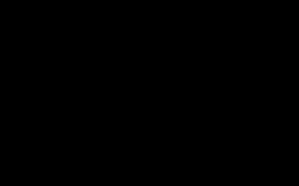
\includegraphics[width=0.50\textwidth]{LC21FieldConfig}
  \caption{\label{LC21FieldConfig}
(Color online)~~~
Discretization of a 1\dmn\ field theory.
Horizontal: $\zeit$ coordinate, with lattice sites marked by dots and
labelled by $\zeit\in\integers$.
(a)
A periodic field $\ssp(\zeit)$, plotted as a function of continuous
coordinate $\zeit$.
(b)
A corresponding discretized period-$5$ {\lattstate}
$\Xx=\cycle{\ssp_0 \ssp_1 \ssp_2 \ssp_3 \ssp_4}$,
with discretized field $\ssp_\zeit$ plotted as a bar
centred at lattice site $\zeit$.
In what follows we use `lattice units' \(a=1\).
          }
\end{figure}
%%%%%%%%%%%%%%%%%%%%%%%%%%%%%%%%%%%%%%%%%%%%%%%%%%%%%

A scalar field $\ssp(x)$ over $d$ Euclidean coordinates can be
discretized by
replacing the continuous space by a $d$\dmn\ hypercubic {integer lattice}
$\lattice$, with lattice spacing $a$, and
evaluating the {field} only on the
lattice points\rf{MonMun94,MunWal00}
\beq
\ssp_z
=
\ssp(x)
    \,,\qquad \qquad x = az= \mbox{lattice point}
    \,,\quad z \in \integers^d
\,,
\ee{LattField}
see \reffig{LC21FieldConfig}.
A given {\em field configuration} (here in one {\spt} dimension)
\beq
\Xx =
\cdots {\ssp}_{-3} {\ssp}_{-2}\,{\ssp}_{-1}\,
       {\ssp}_0\,
      {\ssp}_{1} {\ssp}_{2} {\ssp}_{3} {\ssp}_{4}  \cdots
\,,
\ee{stateSp}
taking any value in system's $\infty$\dmn\ \emph{\statesp}
$\ssp_{z}\in\reals$, occurs with probability
\beq
p(\Xx)\,=\, \frac{1}{Z}\,\e^{-\action[\Xx]}
\,,\qquad Z=Z[0]
\,.
\label{ProbConf}
\eeq
Here $Z$ is a normalization factor, given by the \emph{partition
function}, the integral over probabilities of all
configurations,
\beq
Z[\source]	% = e^{W[\source]}
    \,=\, \int d\Xx\,e^{-\action[\Xx] + \Xx \cdot \source}
    \,,\qquad
d\Xx = \prod_{z}^{\lattice} d\ssp_z
\,,
\ee{partFunct}
where $\source=\{\Ssym{z}\}$ is an external `source' that one can vary
at will, site-by-site, and $\action[\Xx]$ is the action that defines the
theory. %\rf{FieldThe}
The dimension of the partition function integral is the number of lattice
sites $N_\lattice$.
%, \ie, the lattice volume.   % =\Det\lattice$.

Motivated by WKB `semi-classical' or saddle-point
approximations\rf{gutbook} to the partition function \refeq{partFunct},
in this paper we describe their deterministic underpinning, the corresponding
\emph{deterministic} field theory, with partition function built from
solutions to the variational saddle-point condition
\beq
F[\Xx_c]_z =
\action[\Xx_c]_z - \Ssym{z} =0
\,,\qquad
\action[\Xx]_z=\frac{\delta{\action[\Xx]}}{\delta\ssp_z~}
\,,
\ee{LC21eqMotion}
with a global deterministic solution $\Xx_c$ satisfying this local extremal
condition on every lattice site.
In order to distinguish a \emph{solution} to the Euler–Lagrange equations
\refeq{LC21eqMotion} from an {arbitrary} \emph{field configuration}
\refeq{stateSp}, we refer to the solutions as
\emph{{\lattstate}s}, each a set of lattice site field values
\beq
\Xx_c = \{\ssp_z\}
\,,
\label{1dLattStat}
\eeq
that satisfies the local {condition} \refeq{LC21eqMotion} globally,
over all lattice sites.
For a finite lattice segment $\Xx$, one needs to specify the boundary
conditions ({\bcs}).
%  for the Green's function \refeq{tempCatGreen}.
The companion article \refref{GHJSC16} tackles the Dirichlet {\bcs}, a
difficult, time-translation symmetry breaking, and from the \po\ theory
perspective, a wholly unnecessary, self-inflicted pain. All that one
needs to solve the {\templatt} are the $\cl{}$-periodic,
time-translation enforced {\bcs} that we shall use here.
    \PC{2020-02-08}{
Complain about that stupidity clearly both in the intro and in conclusions.
    }
An example is the 1 {\spt} dimension \brick\ of fields of period
$\cl{}=5$ sketched in \reffig{LC21FieldConfig}\,(b),
\beq
\Xx_c = \cycle{\ssp_0 \ssp_1 \ssp_2 \ssp_3 \cdots \ssp_{\cl{}-1}}
\,,
\ee{1dLattStatC_n}
with its infinite repetition --for a sketch, see
\reffig{fig:1dLatStatC_5}\,(1)-- denoted by an overbar.
The first field value $\ssp_0$ in the \brick\ is evaluated on the lattice site 0,
the second $\ssp_1$ on the lattice site 1,
the $(\cl{}+1)$th $\ssp_{\cl{}}=\ssp_0$ on the lattice site $\cl{}$,
with $k$th lattice site field value $\ssp_{k}=\ssp_{\ell}$,
where $\ell=k$~(mod $\cl{}$).

What we call here a chaotic `field' at a discretized spacetime lattice
site $z$, a solid state physicist would call the state of a `particle' at
crystal site $z$, coupled to its nearest neighbors. A solid state
physicist endeavours to understand $N$-particle chaotic systems in
many-body or `large $N$' settings, where in practice any $N$ larger than 2
is `large'. Chaotic field theory is {\em ab initio} formulated for infinite
time and infinite space lattice, but its periodic theory description is
-thanks to hyperbolicity-- computationally powerful already for $N=2, 3,
\cdots$, where $N$ is the number of sites in Bravais cells that tile the
spacetime.

Each {\lattstate} is a distinct deterministic solution $\Xx_c$ to the
discretized Euler–Lagrange equations \refeq{LC21eqMotion}, so its
probability is a $N_\lattice$\dmn\ Dirac delta function
(that's what we mean by the system being \emph{deterministic})
\beq
p_c(\Xx)\,=\, \frac{1}{Z}\,\delta(F[\Xx_c-\Xx])
\,.
\label{DiracDeltaExp}
\eeq

% To comfort sceptics, we verify
In \refsect{s:LC21notHill} we  verify that this
definition agrees with the customary for\-ward-in-time \FP\ probability
evolution\rf{CBmeasure} (see \toChaosBook{section.19.2}{sect.~19.2}). The
new, field-theoretical formulation is vastly preferable to the
for\-ward-in-time formulation when it comes to higher \spt\
dimensions\rf{CL18}.

As is case for a WKB approximation\rf{gutbook}, the {deterministic} field
theory partition sum has support only on lattice field values that are
solutions to the variational saddle-point condition \refeq{LC21eqMotion},
and the partition function \refeq{ProbConf} is now a sum over
configuration \statesp\ \refeq{stateSp} \emph{points},
\bea
Z_c[\source] &=& \sum_c e^{N_\lattice W_c[\source]}
            \continue
e^{N_\lattice W_c[\source]}
    &=& \int_{\pS_c} d\Xx\,\delta(F[\Xx])
    \,=\, \frac{1}{\left|\Det\jMorb_c\right|}
\,,
\label{ClassPartitF}
\eea
where $\pS_c$ is a small neighborhood of  $\Xx_c$, and we refer to
the $[N_c\!\times\!N_c]$ matrix of second derivatives
\beq
(\jMorb_c)_{z'z} = \frac{\delta F[\Xx_c]_{z'}}{\delta \ssp_{z}}
             = \action[\Xx_c]_{z'z}
\ee{jacobianOrb}
as the \emph{\jacobianOrb}.

In what follows, we shall almost exclusively deal only with deterministic field
theory and omit the subscript `$c$' in $\Xx_c$ througout.

\subsection{Lattice Laplacian}
\label{s:LC21lattLap}


Let's have a look at the lattice free field theory action
\beq
\action_0[\Xx]=
          \frac{1}{2}\transp{\Xx}\left(-\Box + {\mu}^2\mathsf{1} \right)\Xx
\,,
\ee{LC21freeAction}
where the `discrete Laplace operator', `central difference operator', or
the `graph Laplacian'%
\rf{PerViv,Pollicott01,Cimasoni12,MraRin12,GodRoy13,Pozrikidis14}
\beq
\Box\,\ssp_z =
    % \frac{1}{2d}
    \sum_{||z'-z||=1} \!\! (\ssp_{z'} - \ssp_z)
 \quad \mbox{for all} \ z,z' \in \lattice % \integers^d
% \,,\quad ||i||:=\sum_{k=1}^{d}|i_k|
% \,,
\ee{LC21:Lap}
is the average of the lattice field variation $\ssp_{z'}-\ssp_z$
over the sites nearest to the site $z$.
For example, for a hypercubic lattice in one and two dimensions this
discretized Laplacian is given by
\bea
\Box\,\ssp_\zeit &=& \ssp_{\zeit+1} - 2\,\ssp_{\zeit} + \ssp_{\zeit-1}
    \label{LC21LaplTime}\\
\Box\,\ssp_{j\zeit}
     &=&
\ssp_{j,\zeit+1} + \ssp_{j+1,\zeit} - 4\,\ssp_{j\zeit}
                 + \ssp_{j,\zeit-1} + \ssp_{j-1, \zeit}
\,.
\label{LC21LaplSpaceTime}
\eea

For action \refeq{LC21freeAction} this is the discretized
{\sPe}\rf{FetWal03}, also known as the {Yukawa} or Klein–Gordon
equation, where  ${\mu}^2>0$ is the Klein–\-Gordon mass-squared.

\subsection{1\dmn\ lattice field theories}
\label{s:LC21FT1d}

Discrete time evolution is frequently recast into a 1\dmn\ temporal
lattice field theory form, essentially by anyone who rewrites a
dynamical systems discrete time evolution problem as a $k$-point recurrence,
for example in
\refrefs{FeHa82,noisy_Fred,conjug_Fred,diag_Fred}.
As already in one \spt\ dimension there is much to be learned about the
role symmetries play in solving lattice field theories, that is what we
will focus on in this paper (time-reversal
\refsects{s:latt1d}{sect:LC21Lind1d}), with the $2$\dmn\ \spt\ field
theories discussed in the sequel\rf{CL18}.

We shall consider scalar field theories of polynomial type, with a local
potential%
\rf{FriMil89,DulMei00,LiMal04,AnBoBa17,AnBoBa18,Anastassiou21}
\beq
V(\ssp_\zeit,\Ssym{\zeit}) =  \frac{g}{k}\ssp_{\zeit}^k
                            - \ssp_{\zeit}^2 -\Ssym{\zeit}\,\ssp_\zeit
\ee{polynPotent}
added to the Laplacian in \refeq{LC21freeAction} on each lattice
site $\zeit$. The discrete Euler–Lagrange equations \refeq{LC21eqMotion}
now take form of 3-term recurrence, second-order difference equations
\bea
- \ssp_{\zeit+1} + V'(\ssp_\zeit,\Ssym{\zeit}) - \ssp_{\zeit-1}
    &=&
0  % was \Ssym{\zeit}
\,.  %\qquad  \ssp_{\zeit} \in [0,1)
\label{LC21:1dTempFT}% \refeq{LC21:1dTempFT}
\eea

We start with the first order difference equation that we call
`{temporal Bernoulli}' (\refsect{s:coinToss}),
\bea
- \ssp_{\zeit+1} + {s}\,\ssp_{\zeit}
    \qquad\quad\;
    &=&
\Ssym{\zeit}
%\,,\qquad  \ssp_{\zeit} \in [0,1)\,,
\label{LC21:1dBernLatt}    % labelled {1stepDiffEq} elsewhere
\eea
in order to motivate the second-order difference
Euler–Lagrange equations \refeq{LC21:1dTempFT}
that we call, in the cases considered here,
the `{\templatt}' (\refsect{s:kickRot}),
`{\henlatt}' (\refsect{s:henlatt}), and
`temporal {$\phi^4$} theory'  (\refsect{s:phi4latt}), respectively:
\bea
- \ssp_{\zeit+1}  +  \,{s}\,\ssp_{\zeit} - \ssp_{\zeit-1}
    &=&
\Ssym{\zeit}
%\,,\qquad  \ssp_{\zeit} \in [0,1)
\label{LC21:1dTemplatt}\\
- \ssp_{\zeit+1} + {a}\,\ssp_{\zeit}^2 - \ssp_{\zeit-1}
    &=&
\Ssym{\zeit}
%\,,\qquad  \Ssym{\zeit}=2
\label{LC21:1dHenlatt}\\
- \ssp_{\zeit+1} + {g}\,\ssp_{\zeit}^3 - \ssp_{\zeit-1}
    &=&
\Ssym{\zeit}
%\,.
\label{LC21:1dPhi4}
\eea
Qualifier `temporal' is used here to emphasize that we view 1\dmn\
examples as special cases of `\spt' field theories; much of our
methodology for $d$\dmn\ deterministic field theories can be profitably
explained by working out $1$\dmn\ field theories.
Lurking here is the totality of the map-iteration dynamical systems
theory, but the reader will find it more profitable, and less confusing,
to think of these simply as lattice problems, and forget that the index
$\zeit$ often stands for `time'.

So, what is a `chaotic', or `turbulent' field theory?
As we shall see, all of the above, as well as their
higher\dmn\ \spt\ siblings are `chaotic' for sufficiently strong `stretching
parameters' or `coupling constants'  ${s}$, ${a}$ or ${g}$.
Our goal here is to make this `{\spt} chaos' tangible and precise, by
acquainting the reader what we believe are
some of the simplest, most elegant examples chaotic field theories.

    \ifboyscout\clearpage\fi
% siminos/reversal/Bernoulli.tex      pdflatex LC21; bibtex LC21
% temporary: siminos/spatiotemp/chapter/LC21Bernoulli.tex
% $Author: predrag $ $Date: 2021-12-24 01:25:20 -0500 (Fri, 24 Dec 2021) $

\section{A fair coin toss}
\label{s:coinToss}
\renewcommand{\ssp}{\ensuremath{x}}               % state space point

The very simplest example of a deterministic law of evolution that gives
rise to `chaos' is the {\em Bernoulli} map, \reffig{fig:BernPart}\,(a),
which models a
\HREF{https://www.random.org/coins/?num=2&cur=40-antique.aurelian} {coin
toss}. Starting with a random initial state, the map generates,
deterministically,  a sequence of tails and heads with the 50-50\%
probability.

We introduce the model in its conventional, time-evolution dynamical
formulation, than reformulate it as a lattice field theory, solved by
enumeration of all admissible \emph{{\lattstate}s}, field configurations that
satisfy a  global fixed point condition, and use this simple setting to
motivate
(1) the \emph{fundamental fact}: for a given lattice period, the {\em
\HillDet} of stabilities of global solutions counts their number
(\refsect{sect:fundFact}), and
(2) the {\tzeta} counts their translational symmetry group orbits
(\refsect{s:PoThe}).

\subsection{Bernoulli map} %Doubling map}
\label{s:Bernoulli}
%ChaosBook return to
% \example{Bernoulli shift map \statesp\ partition.}{ \label{exam:BernMap}

%\renewcommand{\statesp}{state space}
%\renewcommand{\Statesp}{State space}
%\renewcommand{\stateDsp}{state-space}
%\renewcommand{\StateDsp}{State-space}

%
%%%%%%%%%%%%%%%%%%%%%%%%%%%%%%%%%%%%%%%%%%%%%%%%%%%%%%%%%%%%%
\begin{figure}
  \centering
{(a)}
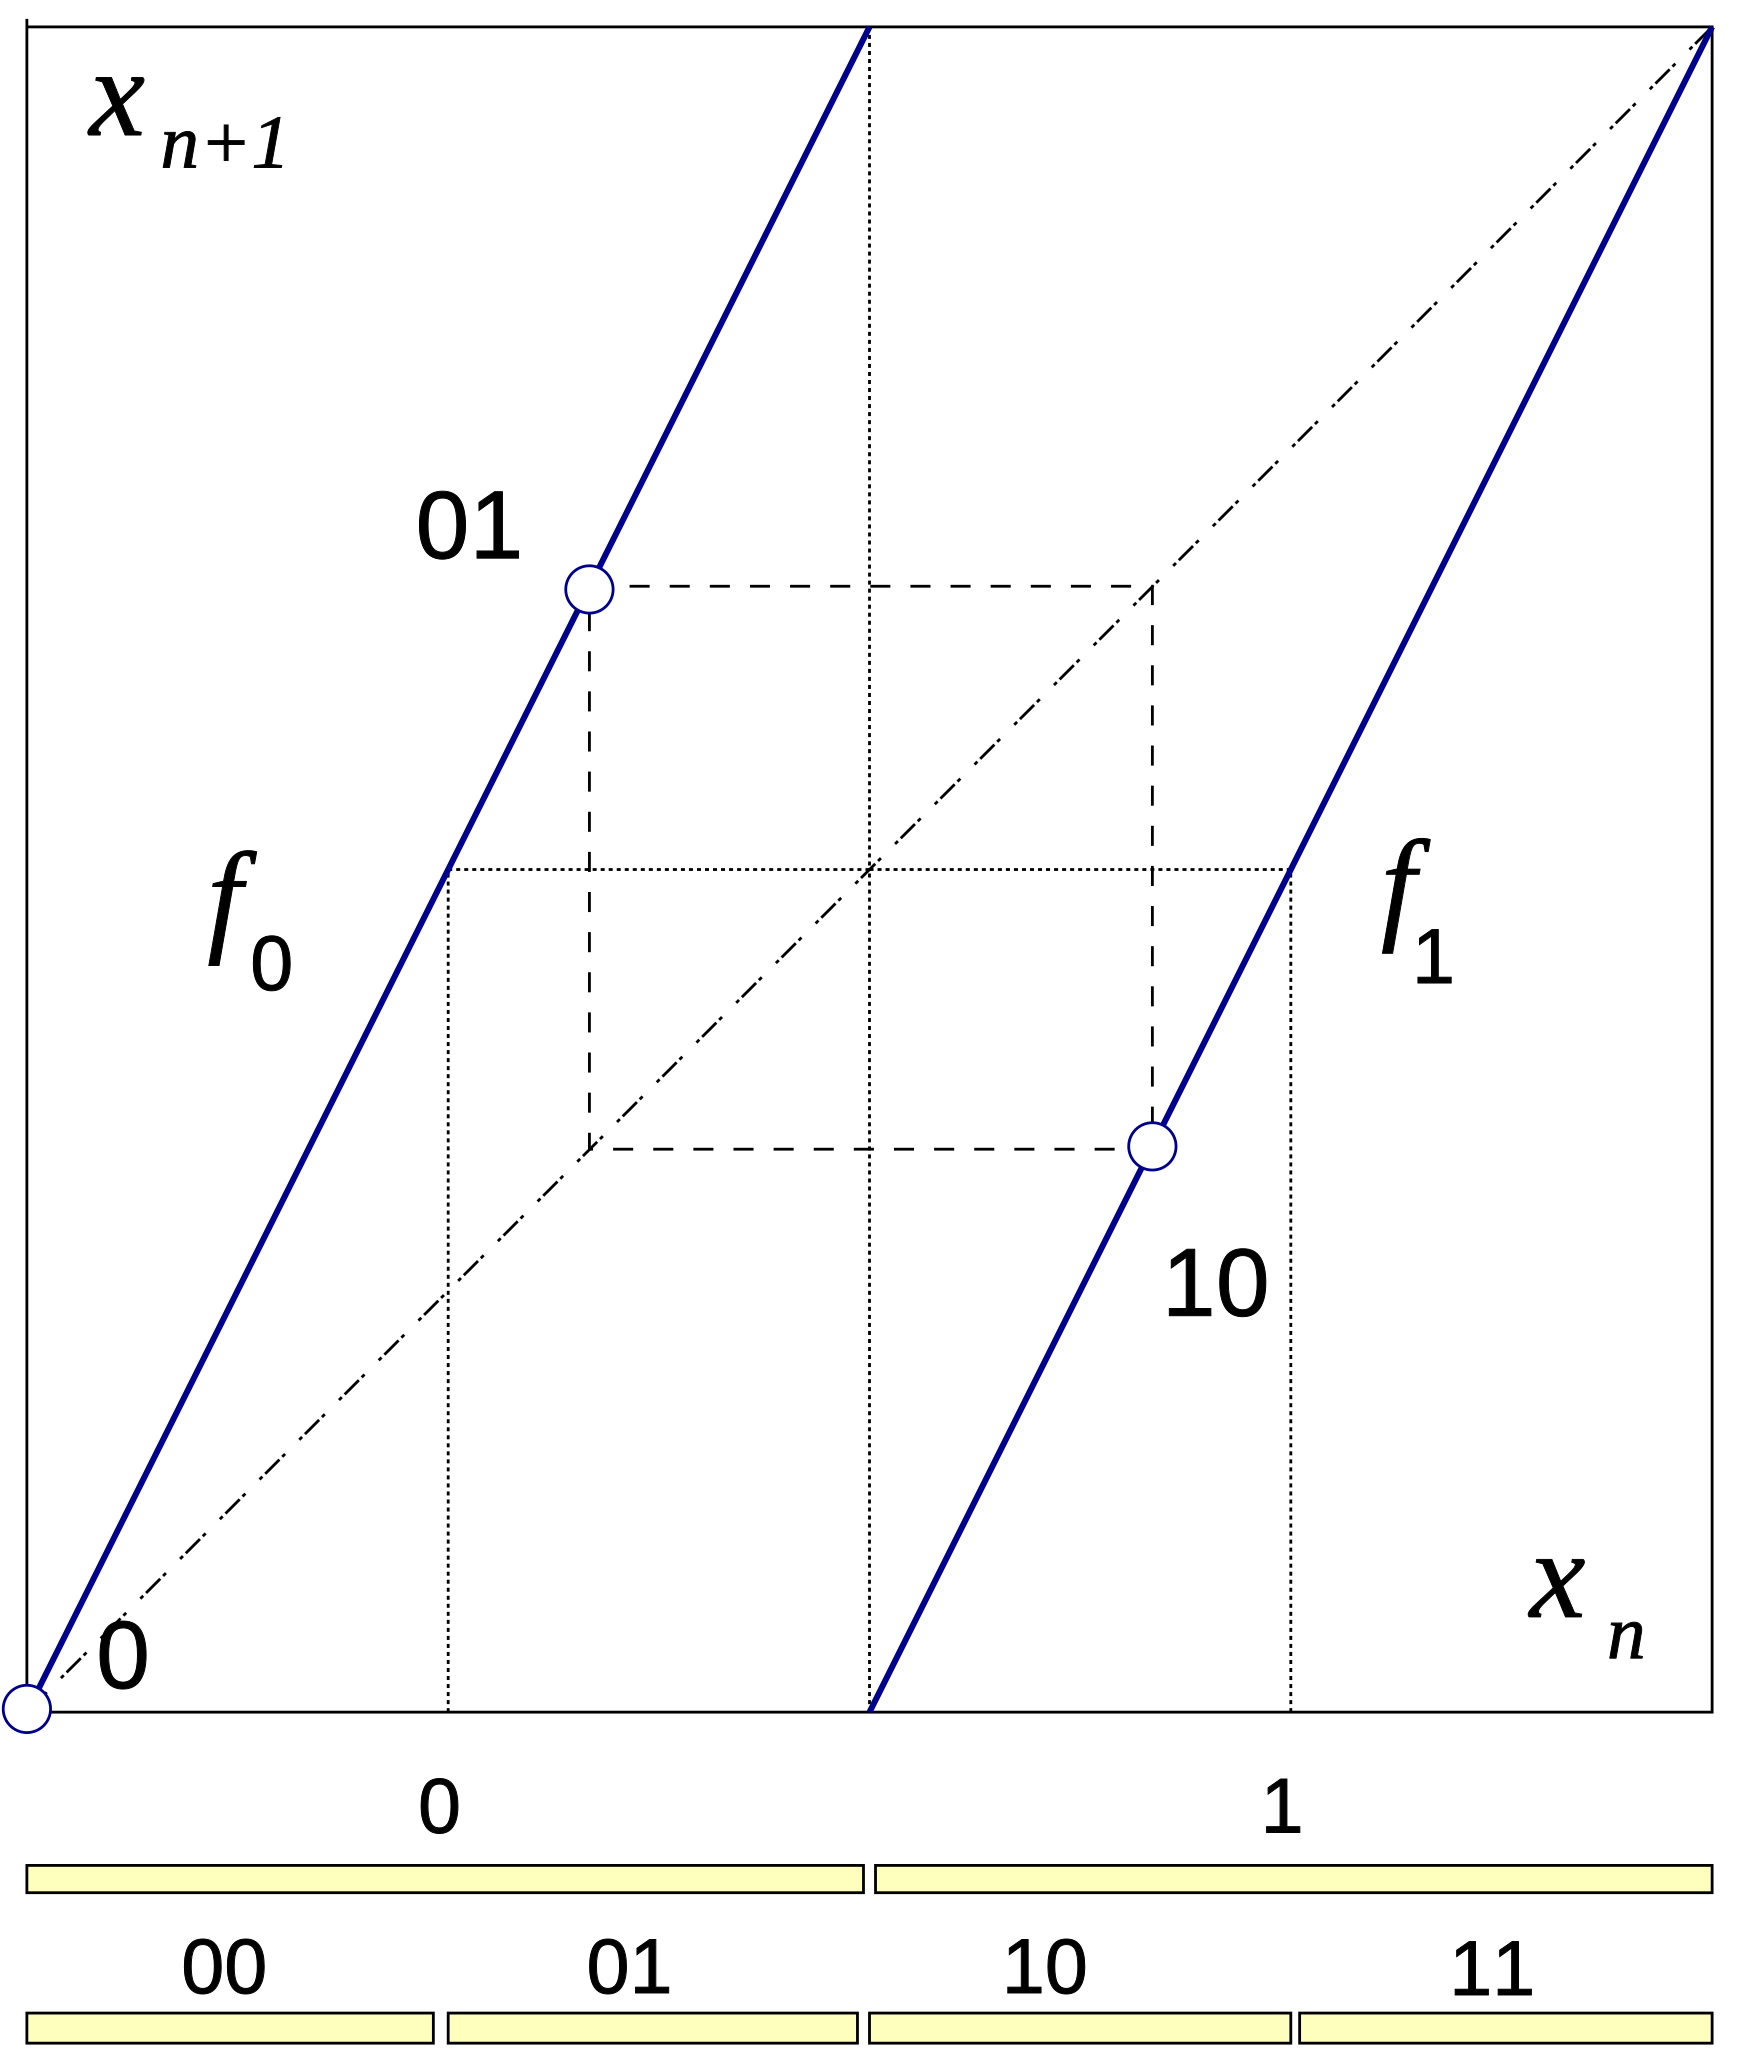
\includegraphics[width=0.35\textwidth]{BernPartCL18}
~~~
{(b)}$\!\!\!\!$
\includegraphics[width=0.40\textwidth]{fig_d_2CL18}

  \caption{\label{fig:BernPart}
(Color online)~~~
(a)
The `coin toss' map \refeq{BerShift}, together with the
$\cycle{0}$ fixed point, and the \cycle{01} 2-cycle. Preimages
of the critical point $\ssp_c=1/2$ partition the unit interval into
$\{\pS_0,\pS_1\}$, $\{\pS_{00},\pS_{01},\pS_{10},\pS_{11}\}$, $\dots$,
subintervals.
(b)
The base-${s}$ Bernoulli map, here with the `dice throw' stretching parameter ${s}=6$,
partitions the unit interval into $6$ subintervals $\{\pS_{\Ssym{}}\}$,
labeled by the ${6}$-letter alphabet \refeq{base-sAlph}. As the map is a
circle map, $\ssp_{5}=1=0=\ssp_{0} \quad(\mbox{mod}\;1)$.
          }
\end{figure}
%%%%%%%%%%%%%%%%%%%%%%%%%%%%%%%%%%%%%%%%%%%%%%%%%%%%%%%%%%%%%%
%

The base-2 {\em Bernoulli} shift map,
\index{Bernoulli!shift}
\index{shift!Bernoulli}
\beq
\ssp_{\zeit+1} =
% \flow{}{\ssp_{\zeit}} =
\left\{ \begin{array}{ll}
        f_0(\ssp_{\zeit}) =  2 \ssp_{\zeit} \,, \quad
                                    & \ssp_{\zeit} \in \pS_0=[0,1/2) \\
        f_1(\ssp_{\zeit}) =  2 \ssp_{\zeit} \;\; (\mbox{mod}\;1)\,, \quad
                                    & \ssp_{\zeit} \in \pS_1 =[1/2,1)
         \end{array}\right.
\,,
\ee{BerShift}
is shown in \reffig{fig:BernPart}\,(a).
If the linear part of such map has an integer-valued slope,
or `stretching' parameter $s\geq2$,
\beq
\ssp_{\zeit+1} \,=\, {s} \ssp_{\zeit}
\ee{BerStretch}
that maps state $\ssp_{\zeit}$ into a state in the `extended \statesp',
outside the unit interval,
the $(\mbox{mod}\;1)$ operation results in the base-${s}$ Bernoulli
circle map,
\renewcommand{\ssp}{\ensuremath{\phi}}             % lattice site field
\beq
\ssp_{\zeit+1}
% = \flow{}{\ssp_{\zeit}}
= {s} \ssp_{\zeit}
\;\; (\mbox{mod}\;1)
%    \,,\qquad \qquad \ssp_{\zeit}\in [0,1)
\,,
\ee{n-tuplingMap}
sketched as a \HREF{https://www.random.org/dice/}{dice throw} in
\reffig{fig:BernPart}\,(b).
The $(\mbox{mod}\;1)$ operation subtracts
$\Ssym{\zeit}=\left\lfloor{s}\ssp_{\zeit}\right\rfloor$, the integer part of ${s}
\ssp_{\zeit}$, or the circle map \emph{winding number}, to keep
$\ssp_{\zeit+1}$ in the unit interval $[0,1)$, and partitions the unit
interval into ${s}$ subintervals $\{\pS_\Ssym{}\}$,
\beq
\ssp_{\zeit+1}
% = \flow{}{\ssp_{\zeit}}
% = \hflow{}{\ssp_{\zeit}} - \Ssym{\zeit+1}
= {s} \ssp_{\zeit} - \Ssym{\zeit}
\,,\qquad  \ssp_{\zeit}\in\pS_{\Ssym{\zeit}}
\,,
\ee{circ-m}
where $\Ssym{\zeit}$ takes values in the ${s}$-letter alphabet
\beq
\Ssym{} \in \A=\{0,1,2,\cdots,s-1\}
\,.
\ee{base-sAlph}

The Bernoulli map is a highly instructive example of a
hyperbolic dynamical system. Its symbolic dynamics is simple:
the base-${s}$ expansion of the initial point $\ssp_0$ is also its
temporal itinerary, with symbols from alphabet \refeq{base-sAlph}
indicating that at time $\zeit$ the orbit visits the subinterval
$\pS_{\Ssym{\zeit}}$. The map is a `shift':
a multiplication by ${s}$ acts on the base-${s}$
representation of $\ssp_{0}=.\Ssym{1}\Ssym{2}\Ssym{3}\cdots $ (for
example, binary, if ${s}=2$) by shifting its digits,
\bea
\ssp_{1}
    &=& \map(\ssp_{0})
    =.\Ssym{2}\Ssym{3}\cdots
%\continue
%\ssp_{\Ssym{2}\Ssym{3}\cdots}
%    &=& \shift{}\,\ssp_{\Ssym{1}\Ssym{2}\Ssym{3}\cdots}
\,.
\label{shiftBern}
\eea

Periodic points can be counted by observing that the preimages of
critical points $\{\ssp_{c1},\ssp_{c2},\cdots\ssp_{c,s-1}\}$ =
$\{{1}/s,{2}/s,\cdots,(s-1)/s\}$ partition the unit interval into
$\{\pS_0,\pS_1,\cdots,\pS_{s-1}\}$, $\{\pS_{\Ssym{1}\Ssym{2}}\}$, $\dots$,
$s^\cl{}$ subintervals, each containing {\em one}  unstable
period-$\cl{}$ periodic point
$\ssp_{\Ssym{1}\Ssym{2}\cdots\Ssym{\cl{}}}$, with stability multiplier
${s}^\cl{}$, see \reffig{fig:BernPart}. The Bernoulli map is a
full shift, in the sense that every itinerary is \admissible, with one
exception: on the circle, the rightmost fixed point is the same as the
fixed point at the origin, $\ssp_{s-1}=\ssp_{0}\quad(\mbox{mod}\;1)$,
so these fixed points are identified and counted as one, see
\reffig{fig:BernPart}. The total number of periodic points of period
$\cl{}$ is thus
\beq
N_{\cl{}} = s^{\cl{}} - 1
\,.
\ee{noPerPtsBm}


\subsection{Temporal Bernoulli}
\label{s:1D1dLatt}

To motivate our formulation of a \spt\ chaotic field theory to be
developed below, we now recast the local initial value, time-evolution
Bernoulli map problem as a \emph{temporal lattice} fixed point condition,
the problem of enumerating and determining all global solutions.

`Temporal' here refers to the lattice site field  $\ssp_\zeit$ and the
source (winding number) $\Ssym{\zeit}$ taking their values on the lattice
sites of a 1\dmn\ \emph{temporal} integer lattice $\zeit\in\integers$.
Over a finite lattice segment, these can be written compactly  as a
\emph{{\lattstate}} and the corresponding \emph{symbol \brick}
\beq
\transp{\Xx} % = \{\ssp_j\}
             = (\ssp_{\zeit+1},\cdots,\ssp_{\zeit+\cl{}})
\,,\quad
\transp{\Mm} % = \{\Ssym{j}\}
             = (\Ssym{{\zeit+1}},\cdots,\Ssym{{\zeit+\cl{}}})
\,,
\ee{pathBern}
where $\transp{(\cdots)}$ denotes a transpose.
The Bernoulli equation \refeq{circ-m}, rewritten as a first-order
difference equation
% \refeq{LC21:1dBernLatt}
\beq
-\ssp_{\zeit+1} + {s}\ssp_{\zeit} - \Ssym{\zeit} =0
\,,\qquad  \ssp_{\zeit} \in [0,1)
\,,
\ee{1stepDiffEq}  % called {...1dBernLatt} elsewhere
takes the matrix form
\beq
\jMorb\,\Xx - \Mm =0
\,,\qquad
\jMorb =  - {\shift} + {s}\id
% former \ee{tempBernFix}
\,,
\ee{tempBern}
where the $[\cl{}\!\times\!\cl{}]$ matrix
\beq
\shift_{jk}=\delta_{j+1,k}
\,,\qquad
\shift
=  \left(\begin{array}{ccccc}
             0    &  1    &        &   &  \cr
                  &  0    &   1    &   &  \cr
                  &       &        & \ddots &  \cr
                  &       &        & 0 & 1 \cr
             1    &       &        &   & 0
          \end{array} \right)
\,,
\ee{hopMatrix}
implements the shift operation \refeq{shiftBern}, a cyclic permutation
that translates for\-ward-in-time {\lattstate} $\Xx$ by one site,
$\transp{(\shift \Xx)}=(\ssp_2,\ssp_3,\cdots,\ssp_\cl{},\ssp_1)$. The
time evolution law \refeq{circ-m} must be of the same form for all times,
so the {\shiftOp} $\shift$ has to be time-translation invariant, with
$\shift_{\cl{}+1,\cl{}}=\shift_{1\cl{}}=1$ matrix element enforcing the
periodicity.

As the {temporal Bernoulli} condition \refeq{tempBern} is a linear
relation, a given \brick\ $\Mm$, or `code' in terms of alphabet
\refeq{base-sAlph}, corresponds to a unique temporal {\lattstate} $\Xx$.
That is why Percival and Vivaldi\rf{PerViv} refer to such symbol \brick\
$\Mm$ as a {\em linear code}.

\subsection{Bernoulli as a continuous time dynamical system}
\label{s:bernODE}

The discrete time derivative of a lattice configuration \Xx\ evaluated at the
lattice site \zeit\ is given by the {difference operator}\rf{Elaydi05}
    \index{lattice!derivative}\index{derivative, lattice}
    \index{lattice!derivative, forward}\index{difference operator}
\beq
\dot{\ssp}_\zeit =
\left[\frac{\partial\Xx}{\partial\zeit}\right]_\zeit
        =
    \frac{\ssp_{\zeit+1} - \ssp_{\zeit}}{\Delta\zeit}
\,.
\ee{lattTimeDer}
The {temporal Bernoulli} condition \refeq{tempBern} %{1stepDiffEq}
can be thus viewed as a time-discretized, first-order ODE dynamical
system
\beq
   \dot{\Xx} \,=\, \vel(\Xx,\Mm) \,,
\ee{1stepVecEq}
where the `velocity' vector field $\vel$ is given by
\[
\vel(\Xx,\Mm) \,=\,
   % \vel(\Xx;\Mm) \,=\,
(s-1)\,\Xx-\Mm
\,,
\]
with the time increment set to $\Delta\zeit=1$, and perturbations that
grow (or decay) with rate $({s}-1)$. By inspection of
\reffig{fig:BernPart}\,(a), it is clear that for \emph{shrinking},
${s}<1$  parameter values the orbit is stable for\-ward-in-time, with a
single linear branch, 1-letter alphabet $\A=\{0\}$, and the only
{\lattstate}s being the single fixed point  $\ssp_0=0$, and its repeats
$\Xx=(0,0,\cdots,0)$. However, for \emph{stretching},  ${s}>1$  parameter
values, the Bernoulli system (more generally, R{\'e}nyi's beta
transformations\rf{Renyi57}) that we study here, every {\lattstate}
$\Xx_\Mm$ is unstable, and there is a {\lattstate} for each admissible
symbol \brick\ \Mm.

\paragraph{A fair coin toss, summarized.}
We refer to the \emph{global} temporal lattice condition \refeq{tempBern}
as the `\emph{temporal} Bernoulli', in order to distinguish it from the
one-time step Bernoulli evolution \emph{map} \refeq{n-tuplingMap}, in
preparation for the study of \emph{\spt} systems to be undertaken in
\refref{CL18}. In the lattice formulation, a \emph{global} {temporal
{\lattstate}} $\Xx_\Mm$ is determined by the requirement that the
\emph{local} temporal lattice condition \refeq{1stepDiffEq} is satisfied
at every lattice site. In \spt\ formulation there is no need for
for\-ward-in-time, close recurrence searches for the returning periodic
points. Instead, one determines each global {temporal {\lattstate}}
$\Xx_\Mm$ at one go, by solving the fixed point condition
\refeq{tempFixPoint}. The most importantly for what follows, the \spt\
field theory of \refref{CL18}, this calculation requires no recourse to any
\emph{explicit coordinatization and partitioning of system's state
space}, and \emph{no explicit symbolic dynamics}.
    \PC{2020-12-17}{
Link to the ChaosBook. Maybe refer to \AW.
    }

%%%%%%%%%%%%%%%%%%%%%%%%%%%%%%%%%%%%%%%%%%%%%%%%%%%%%%%%%%%%%%%%%%%%%%%
%\renewcommand{\statesp}{phase space}
%\renewcommand{\Statesp}{Phase space}
%\renewcommand{\stateDsp}{phase-space}
%\renewcommand{\StateDsp}{Phase-space}

% siminos/reversal/cat.tex      pdflatex LC21; bibtex LC21
% temporary: siminos/spatiotemp/chapter/LC21cat.tex
% $Author: predrag $ $Date: 2021-12-24 01:25:20 -0500 (Fri, 24 Dec 2021) $

\section{A kicked rotor}
\label{s:kickRot}

Temporal Bernoulli is the simplest example of a chaotic lattice field
theory. Our next task is to formulate a deterministic {\spt}ly chaotic
field theory, Hamiltonian and energy conserving, because (a) that is
physics, and (b) one cannot do quantum theory without it. We need a
system as simple as the Bernoulli map, but mechanical. So, we move on
from running in circles, to a mechanical rotor to kick.

The 1-degree of freedom maps that describe kicked rotors
subject to discrete time sequences of angle-dependent force pulses
$P(\coord_{\zeit})$, $\zeit\in\integers$,
\bea
\coord_{\zeit+1} &=& \coord_{\zeit} + p_{\zeit+1} \qquad  (\mbox{mod}\;1),
    \label{LC21PerViv2.1b}\\
p_{\zeit+1}       &=& p_{\zeit} + P(\coord_{\zeit})
\,,
    \label{LC21PerViv2.1a}
\eea
with $2\pi \coord$ the  angle of the rotor, $p$ the momentum conjugate to
the angular coordinate $\coord$, and the angular pulse
$P(\coord_{\zeit})=P(\coord_{\zeit+1})=-V'(\coord_{\zeit})$ lattice
periodic with period $1$, play a key role in the theory of deterministic
and quantum chaos in  atomic physics, from the Taylor, Chirikov and
Greene  standard map\rf{Lichtenberg92,Chirikov79}, to the cat maps that
we turn to now. The equations are of the Hamiltonian form:
eq.~\refeq{LC21PerViv2.1b} is $\dot{\coord}=p/m$ in terms of discrete
time derivative \refeq{lattTimeDer}, \ie, the configuration trajectory
starting at $\coord_{\zeit}$ reaches
$\coord_{\zeit+1}=\coord_{\zeit}+p_{\zeit+1}\Delta{\zeit}/m$ in one time
step $\Delta{\zeit}$. Eq.~\refeq{LC21PerViv2.1a} is the time-discretized
$\dot{p}=-\partial V(\coord)/\partial \coord$: at each kick the angular
momentum $p_{\zeit}$ is accelerated to $p_{\zeit+1}$ by the force pulse
$P(\coord_{\zeit})\Delta{\zeit}$, with the time step and the rotor mass
set to $\Delta{\zeit}=1$,  $m=1$.

%\section{Life of a single Hamiltonian cat}
\subsection{Cat map}
%    \fi
\label{s:catPV}

The simplest kicked rotor is subject to force pulses
$P(\coord)=\kappa\coord$ proportional to the angular displacement
$\coord$: in that case, the map
(\ref{LC21PerViv2.1b},\ref{LC21PerViv2.1a}) is of form
%    \PC{2021-12-26}{I see \refeq{HLHamiltonsEquations} here:)}
 \beq
 \left(\begin{array}{c}
 \coord_{\zeit+1}  \\
   p_{\zeit+1}
  \end{array} \right )=
  \jMat \left(\begin{array}{c}
 \coord_{\zeit}  \\
   p_{\zeit}
  \end{array} \right )\quad (\mbox{mod}\;1)
    \,,  \qquad
 {\jMat} =\left(\begin{array}{cc}
 \kappa+1 & 1 \\
  \kappa & 1
  \end{array} \right)
\,.
\ee{catMap}
The $(\mbox{mod}\;1)$ makes the map a
discontinuous `sawtooth,' unless $\kappa$ is a positive integer.
The map is then a Continuous Automorphism of the Torus
known as the Thom-Anosov-Arnol'd-Sinai
{\em `cat map'}\rf{ArnAve,deva87,StOtWt06}, extensively studied as the
simplest example of a chaotic Hamiltonian system.

The determinant of the one-time-step Jacobian is
$\det \jMat=1$, \ie, the mapping is area-preserving.
Let ${s}=\tr{\jMat}=\kappa+2$ be the trace of the Jacobian.
For $|s|>2$ the $\jMat$ {characteristic equation}
\beq
\ExpaEig^{2} - {s}\ExpaEig + 1 = 0
\,,
\ee{LC21:StabMtlpr}
has real roots
$(\ExpaEig\,,\;\ExpaEig^{-1})$  and a positive Lyapunov exponent
$\Lyap >0$,
\beq
\ExpaEig=e^{\Lyap} = \frac{1}{2}(s+\sqrt{(s-2)(s+2)})
\,,\qquad
{s}=\tr{\jMat}=\ExpaEig+\ExpaEig^{-1}
\,.
\ee{StabMtlpr}
The eigenvalues are functions of the stretching parameter $s$, and
for $|s| > 2$ the cat map \refeq{catMap} is a fully chaotic
Hamiltonian dynamical system.

\subsection{\tempLatt}
\label{s:catLagrange}
    % earlier names:
    % \section{Life of a single Lagrangian cat}
    % \section{Cat map in Lagrangian formulation}
\renewcommand{\period}[1]{{\ensuremath{n_{#1}}}}
    % discrete length of a cycle, Predrag

In order to motivate our formulation of higher-dimensional \spt\ chaotic
field theories, to be developed in \refref{CL18}, we now recast the
\emph{local} initial value, Hamiltonian time-evolution  as a
\emph{global} solution to the Euler–Lagrange equations.

The 2-component field at the
temporal lattice site \zeit,
\(
\ssp_{\zeit} =(\coord_{\zeit},p_{\zeit}) \in  (0,1]\times(0,1]
\)
is kicked rotor's the angular position and momentum.
Hamilton's equations (\ref{LC21PerViv2.1b},\ref{LC21PerViv2.1a}) induce
for\-ward-in-time evolution on a 2-torus  $(\coord_{\zeit},p_\zeit)$ {\em
phase space}.
Eliminating the momentum by Hamilton's discrete time velocity
eq.~\refeq{LC21PerViv2.1b},
\beq
(\coord_\zeit,p_\zeit) =
\left(
    \coord_{\zeit},\frac{\coord_{\zeit} - \coord_{\zeit-1}}{\Delta\zeit}
\right)
%\,,\qquad \Delta\zeit= 1
\,,
\ee{Ham2Lagr}
setting the time step to $\Delta\zeit=1$, and forgetting for a moment
the $(\mbox{mod}\;1)$ condition, the
for\-ward-in-time Hamilton's first order difference equations are brought
to the second order difference, 3-term recurrence Euler–Lagrange equations
for scalar field $\ssp_{\zeit}=q_\zeit$,
\beq
\ssp_{\zeit+1} - 2\,\ssp_{\zeit} + \ssp_{\zeit-1} = P(\ssp_{\zeit})
\,.
\ee{cattyMappo}
But that is Newton's Second Law: ``acceleration equals
force,'' so Percival and Vivaldi\rf{PerViv} refer to this formulation as
`Newtonian'. Here we follow Allroth\rf{Allroth83}, Mackay, Meiss,
Percival, Kook \& Dullin\rf{MacMei83,meiss92,MKMP84,DulMei98,kooknewt},
and Li and Tomsovic\rf{LiTom17b} in referring  to it as `Lagrangian'.

For the cat map \refeq{catMap}, the Lagrangian passage
\refeq{Ham2Lagr} to the  scalar field  $\ssp_{\zeit}$ leads to the \PV\
`two-configuration representation'\rf{PerViv}
\beq
 \left(\begin{array}{c}
 \ssp_{\zeit}  \\
 \ssp_{\zeit+1}
 \end{array} \right )=
 \jMat_{PV} \left(\begin{array}{c}
 \ssp_{\zeit-1}  \\
 \ssp_{\zeit}
 \end{array} \right ) %\mbox{ mod } 1
 - \left(\begin{array}{c}
 0  \\
 \Ssym{\zeit}
 \end{array} \right )
 \,,  \qquad
 {\jMat_{PV}} =\left(\begin{array}{cc}
 0 & 1 \\
 -1 & s
 \end{array} \right ),
%\,.
\ee{LC21PerViv}
with matrix $\jMat_{PV}$ acting on the 2\dmn\ space of successive
configuration points $\transp{(\ssp_{\zeit-1},\ssp_{\zeit})}$. As was
case for the Bernoulli map \refeq{1stepDiffEq}, the cat map
$(\mbox{mod}\;1)$ condition \refeq{catMap} is enforced by integers
$\Ssym{\zeit}\in  \A$, where for a given integer stretching parameter $s$
the alphabet \A\ ranges over $|\A|={s}\!+\!1$ possible values for
$\Ssym{\zeit}$,
\beq
\A=\{\underline{1},0,\dots s\!-\!1\}
\,,
\ee{catAlphabet}
necessary  to keep $\ssp_{\zeit}$ for all times $t$ within the unit
interval $[0,1)$. (We find it convenient to have symbol
$\underline{\Ssym{}}{}_{\zeit}$ denote $\Ssym{\zeit}$ with the negative
sign, \ie, `$\underline{1}$' stands for symbol `$-1$'.)


Written out as a second-order difference equation, the \PV\ map
\refeq{LC21PerViv} takes a particularly elegant form, that we shall
refer to as the {\em \templatt} \refeq{LC21:1dTemplatt},
\beq
-\ssp_{\zeit+1}  +  s \, \ssp_{\zeit} - \ssp_{\zeit-1}
    =
\Ssym{\zeit}
\,,
\ee{catMapNewt}
or,
in terms of a {{\lattstate}} $\Xx$, the corresponding {symbol \brick}
$\Mm$ \refeq{pathBern}, and the $[\cl{}\!\times\!\cl{}]$ {\shiftOp}
$\shift$ \refeq{hopMatrix},
\beq
(-\shift + s\id - \shift^{-1})\,\Xx =  \Mm
\,,
\ee{catTempLatt}
very much like the {temporal Bernoulli} condition \refeq{tempBern}, and
the winding numbers (sources) $\Mm$ taking their values on the lattice
sites of a 1\dmn\ \emph{temporal} lattice $\zeit\in\integers$.
%    \PC{2021-10-13}{Dropped:
%Nonlinearity of the \catlatt\ arises from restricting the admissible
%values of fields $\ssp_z$ to the unit interval.
%    }

As was the case for {temporal Bernoulli} \refeq{tempBern}, the condition
\refeq{LC21PerViv} is a linear relation: a given `code'
$\{\Ssym{\zeit}\}$ in terms of alphabet \refeq{catAlphabet} corresponds
to a unique temporal sequence $\{\ssp_\zeit\}$. That is why Percival and
Vivaldi\rf{PerViv} refer to such symbol \brick\ $\Mm$ as a {\em linear
code}. As for the Bernoulli system, $\Ssym{\zeit}$ can also be
interpreted as `winding numbers'\rf{Keating91}, or, as they shepherd
stray points back into the unit torus, as `stabilising
impulses'\rf{PerViv}. Here we use the field-theoretical parlance,
and refer to them  as `sources'.

                               \toCB

\subsection{\tempLatt\ as a continuous time dynamical system}
\label{s:tempCatODE}

Recall that the Bernoulli first-order difference equation could be viewed as
a time-discretization of the first-order linear ODE \refeq{1stepVecEq}. The
second-order difference equation \refeq{catMapNewt} can be interpreted as the
second order discrete time derivative ${d^2}/{dt^2}$, or the temporal
lattice Laplacian \refeq{LC21LaplTime},
\beq
\Box\,\ssp_\zeit \equiv
\ssp_{\zeit+1} - 2\ssp_{\zeit} + \ssp_{\zeit-1}
= (s-2)\ssp_{\zeit} -\Ssym{\zeit}
\,,
\ee{LC21PerViv2.2}
 with the time step set to $\Delta\zeit=1$.
In other words, if we include the cat map forcing pulse
\refeq{LC21PerViv2.1a}
\(
P(\ssp_\zeit)= - V'(\ssp_\zeit) = - (s-2)\,\ssp + \Ssym{\zeit}
\)
into the definition of
the on-site potential \refeq{LC21:1dTempFT},
\beq
V(\Xx,\Mm) = \sum_{\zeit\in\lattice}\left(
\frac{1}{2}\mu^2\ssp_\zeit^2 -\Ssym{\zeit}\,\ssp_\zeit\right)
\,,
\ee{templattV}
the force
is linear in the angular displacement $\ssp$, so
the \templatt\ Euler-Lagrange equation takes form (see free action
\refeq{LC21freeAction})
\beq
(-\Box + {\mu}^2\id)\,\Xx = \Mm
%\,,  \qquad
%{\mu}^2={s}-2
% \Box\,\ssp_{\zeit}:= \ssp_{\zeit-1}-2\ssp_{\zeit} +\ssp_{\zeit+1}
\,,
\ee{OneCat}
where the Klein-Gordon mass ${\mu}$ is related to the cat-map
stretching parameter ${s}$ by ${\mu}^2={s}-2$.

For small stretching parameter values, $s<2$, this discretized
Euler–\-Lagrange equation \refeq{LC21eqMotion} describes a set of coupled
penduli, with oscillatory solutions, known as the discrete Helmholtz
equation in applied math\rf{DiHaHu01,Lick89,FetWal03}, as  the
tight-binding model, the Harper's or Azbel-Hofstadter model in solid
state physics\rf{Peierls33,MiDuWh92,Cserti00,Economou06,CsSzDa11},  and
the critical almost Mathieu operator in mathematical physics\rf{Simon82},
with quadratic action \refeq{LC21freeAction} written as Hamiltonian
\[ %beq
H=\sum_\ell\ket{\ell}\epsilon_0\bra{\ell}
  + \sum_{\ell m}\ket{\ell}V_{\ell m}\bra{m}
\,,\quad
   V_{\ell m} = \left\{
     \begin{array}{ll}
         V & \mbox{if\ } \ell,m \mbox{ nearest neighbors}\\
         0 & \mbox{otherwise}
     \end{array}
             \right.
\] %ee{Economou06(5.7)}
with the stretching factor ${s}=-\epsilon_0/V$ in
\refeq{LC21PerViv2.2}.
%{OneCat}.

Here we study the strong stretching, $s>2$ case, known as the discrete
\sPe\rf{Dorr70,GoVanLo96,HuCon96,HuRyCo98,FetWal03,Pozrikidis14},
whose solutions are hyperbolic. We refer to the
Euler–\-Lagrange equation
\refeq{OneCat} as the `{\em \templatt}', both to distinguish it from
the for\-ward-in-time Hamiltonian cat \emph{map} \refeq{catMap}, and in the
anticipation of the \emph{\catlatt} to be discussed in the sequel
\refref{CL18}. {\catLatt} differs from all of the above models because the
field $\ssp_\zeit$ compactification to unit circle makes it a
strongly nonlinear deterministic field theory, with nontrivial symbolic
dynamics.

\bigskip

\noindent\textbf{\tempLatt, summarized.}
In the \spt\ formulation a \emph{global} {temporal {\lattstate}}
\beq
\transp{\Xx} % = \{\ssp_j\}
             = (\ssp_\zeit,\ssp_{\zeit+1},\cdots,\ssp_{\zeit+k})
\ee{path}
is not determined by a for\-ward-in-time `cat map' evolution
\refeq{catMap}, but rather by the fixed point condition
\refeq{LC21eqMotion}
% tempCatFixPoint}
that the \emph{local}, 3-term discrete temporal lattice Euler–Lagrange
equations \refeq{catMapNewt} are satisfied at every lattice point. This
temporal 1\dmn\ lattice reformulation is the bridge that takes us from
the single cat map \refeq{catMap} to the higher-\dmn\ coupled
``multi-cat'' \spt\ lattices\refrefs{GutOsi15,GHJSC16,CL18}.

And, did you know that the cute Arnold cat is but the % very fundamental
{\sPe} in disguise? And that the lattice form \refeq{catMapNewt}
of the theory is so much more elegant than the
cat-map form \refeq{catMap}?
A cat is Hooke's wild, `anti-harmonic' sister.
For $s<2$ Hooke rules: restoring oscillations around the sleepy resting
state.
For $s>2$ cats rule: exponential runaway, wrapped globally around a
\statesp\ torus. {Cat} is to {chaos} what {harmonic oscillator} is to
{order}. There is no more fundamental example of chaos in mechanics.


\renewcommand{\period}[1]{{\ensuremath{T_{#1}}}}         %continuous cycle period

% siminos/reversal/LC21nonlinFT.tex      pdflatex LC21; bibtex LC21
% temporary: siminos/spatiotemp/chapter/LC21nonlinFT.tex
% $Author: predrag $ $Date: 2021-12-24 01:25:20 -0500 (Fri, 24 Dec 2021) $

% was \section{Nonlinear lattice field theories}
%\label{s:nonlinFT}

\section{A $\ssp^3$ field theory}
% was {{\Henlatt}}
\label{s:henlatt}

The `mod~1' in the definition of the `linear' kicked rotor, the cat map
\refeq{catMap}, makes cat map a highly nonlinear, discontinuous map. In
contrast, field theory action $\action[\Xx]$ is typically polynomial and
smooth. The simplest such nonlinear action turns out to correspond to the
paradigmatic dynamicist's model of a 2\dmn\ nonlinear dynamical system,
the {\HenonMap}\rf{henon}
\bea
    x_{\zeit+1} &=& 1-a\,x_{\zeit}^2 + b\,y_{\zeit}
        \continue
    y_{\zeit+1} &=& x_{\zeit}
\,.
\label{LC21eq2.1}
\eea
For the contraction parameter value $b=-1$ this is a Hamiltonian map.

The \emph{temporal evolution} \jacobianM\ for the $n$th iterate of the
Hamiltonian {\HenonMap} is the product of consecutive  one time-step
\jacobianMs
\beq
\jMps^\cl{}(x_0,y_0) =
\prod_{m=\cl{}-1}^{0}
            \left(\begin{array}{cc}
                -2a\,x_m & -1 \\
                         1 & 0
            \end{array}\right)
\,,\qquad x_m = \map^{m}_1 (x_0,y_0)
\,,
\ee{Henlatt-e_her}
where the successive 1-time step \jacobianMs\ are multiplied in the order
they are applied, as
$\jMps^\cl{}(x_0)=\jMps(x_{\cl{}-1})\cdots\jMps(x_0)$. So, once we have a
{\HenonMap} {\po}, we also have its \FloquetM\
(monodromy matrix). When $\jMps^\cl{}$ is
hyperbolic, only the expanding
eigen\-value $\ExpaEig_1=1/\ExpaEig_2$ needs to be determined, as the
determinant of the {\Henon} 1-time step \jacobianM\ is unity,
\beq
\det\jMps = \ExpaEig_1 \ExpaEig_2 = 1
\,.
\ee{LC21:HenDet}
The map is Hamiltonian in the sense that it preserves areas in the
$[x,y]$ plane.


The {\HenonMap} is the simplest map that captures chaos that arises from
the smooth stretch \& fold dynamics of nonlinear {\PoincMap}s of flows
such as R\"ossler\rf{ross}.
Written as a  2nd-order inhomogeneous difference equation\rf{DulMei00},
\refeq{LC21eq2.1} takes the
{\em \henlatt} 3-term recurrence form, explicitly time-translation
and time-reversal invariant Euler–Lagrange equation
% \refeq{LC21:1dHenlatt}:
\beq
-\ssp_{\zeit+1} + {a}\,\ssp_{\zeit}^2 - \ssp_{\zeit-1} = 1
\,.
\ee{LC21:2-step}
Just as the kicked rotor (\ref{LC21PerViv2.1b},\ref{LC21PerViv2.1a}), the map can
be interpreted as a kicked driven anaharmonic oscillator\rf{Heagy92},
with the nonlinear, cubic Biham-Wenzel\rf{afind} lattice site potential
\refeq{polynPotent}
\beq
V(\Xx,\Mm) = \sum_{\zeit\in\lattice}\left(
\frac{a}{3}\ssp_{\zeit}^3 -\Ssym{\zeit}\,\ssp_\zeit\right)
    \,,\qquad
        \Ssym{\zeit} = -1
\,,
\ee{LC21BWcubic}
giving rise to kicking pulse \refeq{LC21PerViv2.1a}.
    \PC{2021-12-10} {
Note the cubic Biham-Wenzel potential includes
the source term, as  \refeq{LC21:1dTempFT}.
Please recheck the signs!
    }
Devaney, Nitecki, Sterling and Meiss\rf{Devaney79,StMeiss98,SteDuMei99}
have shown that the Hamiltonian {\HenonMap} has a complete Smale
horseshoe for sufficiently large `stretching parameter' values
\beq
      a > 5.699310786700\cdots
\;.
\ee{LC21:SterlHen}
In numerical\rf{ChaosBook} and analytic\rf{EndGal06} calculations we fix
(arbitrarily) the stretching parameter value to $a=6$, in order to
guarantee that all $2^\cl{}$ periodic points  $\ssp=\flow{\cl{}}{\ssp}$
of the {\HenonMap} \refeq{LC21eq2.1} exist.
    \PC{2021-12-10} {
Explain that $\phi^3$ theory is correspond to the unimodal \henlatt, with
the Smale horseshoe repeller cleanly split into the left (negative) and
right (positive) lattice site field values.
This is very much like the temporal Bernoulli, in contrast to the
\templatt\ which has nontrivial pruning, see \reftab{tab:catMapN_n-s=3}.
    }

    \PC{2021-06-04}{
S. Aubry\rf{aub95ant}
{\em Anti-integrability in dynamical and variational problems}

The \eqva\ and \reqva\ of Frenkel-Kontorova models\rf{AuAb90,MraRin12}, widely studied in
literature, might be closely related to \henlatt\ and $\phi^4$ lattices.



D. G. Sterling\rf{SterlingThesis99}
much (undeservedly)
un-cited \HREF{https://www.proquest.com/docview/304508605} {PhD thesis},
Univ. of Colorado,
{\em Anti-Integrable Continuation and the Destruction of Chaos} has much
to teach us. He studies \emph{coupled {\HenonMap} lattices} in both
Hamiltonian and Lagrangian formulations; his definition seems pretty much
consistent with our \refeq{SVWhenSTlatt}, though he has a coupling
parameter $c$ used to make spatial couplings weak. The
``anti-integrable'' refers to our choice $a\geq6$, I believe - parameter
regimes in which all of the horseshoe orbits exists.

``Specifying the anti-integrable state for an orbit of a coupled map
lattice requires a multidimensional symbolic object which we call a
symbol tensor.''

His Figures 6.7, 6.18 are reminiscent of my pruning front.

Sterling and Meiss\rf{StMeiss98}
{\em Computing periodic orbits using the anti-integrable limit}

    } % end     \PC{2021-06-04}

% \PC{2020-05-31} {
Politi and Torcini\rf{PolTor92} note that
a problem in reconstructing the statistical properties of an
{\spt\ H{\'e}non} attractor
is ensuring that all \twots\  used are embedded into the inertial manifold.
For instance, in the single H{\'e}non map, one
of the two fixed points is isolated and it does not belong to the strange
attractor.

We resolve this problem by construction, all our solutions belong to the
non-wondering set.
%   }

%\section{PolTor92 Periodic orbits in coupled {H{\'e}non} maps}
%\label{sect:PolTor92}
%\item[2020-05-31 Predrag]
Politi and Torcini\rf{PolTor92} {\em Periodic
orbits in coupled {H{\'e}non} maps: {Lyapunov} and multifractal analysis}

They study \emph{\spt\ \Henon}, a (1+1)-spacetime lattice of
\Henon\ maps orbits which are periodic both in space and time.

Their numerical method is an extension of Biham and Wenzel\rf{afind} for
the single \Henon\ map, with symbols $\Ssym{n\zeit}$ in $\A=\{0,1\}$. Any
fixed point in fictitious time corresponds to a spatio-temporal cycle
$\BravCell{\speriod{}}{\period{}}{\tilt{}}$.


\section{A {$\phi^4$} field theory}
\label{s:phi4latt}

If a potential that is bounded from below is needed to make sense of the
probabilistic interpretation of the configuration weight
\refeq{ProbConf}, or a symmetry forbids the odd-power potentials such as
\refeq{LC21BWcubic}, one starts instead with a quartic potential
$\sim{g}\ssp_{\zeit}^4$, leading to the `{$\phi^4$} lattice field theory'
\refeq{LC21:1dPhi4}. As $\phi^4$ example adds little to understanding
over what is learned from \henlatt, we will not discus is further in this
paper.
    \PC{2021-12-10} {
No! Explain that $\phi^4$ theory is the bimodal extension of
what we had learned for the unimodal \henlatt.

The \HenonMap/$\phi^3$ approaches should be safe for multimodal maps with
complete repelling sets, and it should work for finite-grammar Smale
horseshoe repellers.
Smale's original horseshoe\rf{smale}, his fig.~1 was unimodal, but he
also explicitly gives our $\phi^4$ bimodal repeller, his fig.~5.
    }

    \PC{2021-10-13}{RECHECK,
maybe applies to \catlatt: Equilibria or steady solutions of
Frenkel-Kontorova lattices, the smooth function $V:\reals\to\reals$ is a
periodic onsite potential, $V[\ssp+1]=V[\ssp]$ for all $\xi\in\reals$.

%\PC{2019-06-26}{
%Mramor and Rink
The $d$-dimensional Frenkel-Kontorova Hamiltonian lattice differential
equation\rf{AuAb90,MraRin12}
\beq
\frac{d^2 \ssp_i}{dt^2} + V'[\ssp_i] - \Box\,\ssp_i
    = 0 \ \mbox{for all} \ i\in\mathbb{Z}^d.
\ee{LC21FKHam}
describes the motion of particles under the
competing influence of an onsite periodic potential field and nearest
neighbor attraction.

the goal is to find a
$d$-dimensional ``lattice configuration''
(for us, {\lattstate})
$x:\integers^d\to \reals$ that satisfies
\beq
V'[\ssp_i] - \Box\,\ssp_i = 0 \  \ \mbox{for all} \ i\in \mathbb{Z}^d
\,.
\ee{FKeq} %\ref{RR} in {MraRin12}
% \PC{2019-06-26}{
Eq.~\refeq{FKeq}
is relevant for statistical mechanics\rf{MraRin12}, because it is
related to Eq.~\refeq(FKeq) describes its stationary solutions.
%  }
    }


\section{Computing {\lattstate}s for nonlinear theories}
\label{s:nonlinLattStates}

Unlike the {temporal Bernoulli} \refeq{LC21:1dBernLatt} and the
{\templatt} \refeq{LC21:1dTemplatt}, for which the {\lattstate} fixed
point condition \refeq{LC21eqMotion}
% {tempCatFixPoint}
is linear and easily solved, for
nonlinear lattice field theories the {\lattstate}s are roots of
polynomials of arbitrarily high order. While Gallas and collaborators%
\rf{EndGal01,EndGal02,EG05,EG05a,EndGal06,Gallas18,Gallas20,Gallas20a}
have developed a powerful theory that yields {\HenonMap} {\po}s in
analytic form, it would be unrealistic to demand such explicit solutions for
general field theories on multi-dimensional lattices. We take a
pragmatic, numerical route, and search for the fixed-point solutions
\refeq{LC21eqMotion}
starting with the deviation of an approximate trajectory from the 3-term
recurrence \refeq{LC21:1dTempFT}, given by the lattice deviation vector
\beq
v_{\zeit} = -\ssp_{\zeit+1} + (V'(\ssp_{\zeit})-\Ssym{\zeit}) - \ssp_{\zeit-1}
\,,
\ee{LC21BWdeviate}
and minimizing this error term by any convenient variational or
optimization method, perhaps in conjunction with a high-dimensional
variant of the Newton method\rf{CvitLanCrete02,lanVar1}.
    \PC{2021-12-10} {
Form $(V'(\ssp_{\zeit})-\Ssym{\zeit})$ looks like the most convenient
definition of the ``$\Ssym{}$-centered" subregion $\pS_\Ssym{}$ potential,
applicable to both linear and nonlinear field theories?
    }



\subsection{Papers to refer to?}

Sim{\'o}\rf{Simo79} {\em On the {H{\'e}non-Pomeau} attractor}
is a very fine early paper. Cite it in \Henon\ remark.

Miguel, Sim{\'{o}} and Vieir\rf{MiSiVi13} {\em From the {H{\'{e}}non}
conservative map to the {Chirikov} standard map for large parameter
values} \CBlibrary{MiSiVi13}:

Endler and Gallas\rf{EG05}.
method resembles the methods
earlier employed for quadratic polynomials (and their Julia sets) by
Brown\rf{Brown81}
and Stephenson\rf{Stephen1992A}.

Brown gives cycles up to length 6 for the logistic map,
employing symmetric functions of periodic points.

Hitzl and Zele\rf{HitZe85}
study the of the {\HenonMap} for cycle lengths  up to period  6.

    \ifboyscout\clearpage\fi
% siminos/reversal/recip1d.tex      pdflatex LC21; bibtex LC21
% temporary:  siminos/spatiotemp/chapter/LC21recip1d.tex
% $Author: hanliang $ $Date: 2021-12-24 16:09:56 -0500 (Fri, 24 Dec 2021) $

% Predrag 2021-08-08: shared with siminos/reversal/LC21.tex

\section{Reciprocal lattice}
\label{sect:LC21recip1d} % started with {sect:RhombCornerFT}

ChaosBook conventions:
\renewcommand{\cssp}{\ensuremath{\tilde{\phi}}}                % Complex state space point

$\omega = e^{2i\pi/\cl{}}$

$\cssp_k=x_k+i\,y_k = |\cssp_k| e^{i\theta_k}$

$q_k=2\pi{k}/\cl{}$,

$\cl{}$ is the Bravais cell period

\bigskip

Think of a solution of a discrete time dynamical system (iterations of a map) as a
1\dmn\ temporal {\lattstate} with the field on each site labeled by integer
time.
Were the lattice $d$\dmn, defined by Bravais cell vectors $\{\mathbf{a}\}$, a
crystallographer would immediately move to the \emph{reciprocal}
lattice,
\( %beq
\tilde{\lattice}_{\mathbf{b}} = \{k \mathbf{b}\,|\, k \in \mathbb{Z}\}
\,,
\) %ee{LC21:Rcpr1dLatt}
with the {reciprocal}
lattice basis vectors $\{\mathbf{b}\}$ satisfing
\( %beq
\mathbf{b} \cdot \mathbf{a} = 2 \pi
\,.
\) %ee{LC21:Rcpr1dVect}
On the {reciprocal} lattice translations are
quotiented out, and calculations are restricted to a finite
{Brilluoin zone} (this is the {`Bloch theorem'} of
solid state physics). Here we work on a 1\dmn\ lattice with unit
lattice spacing 1, so the reciprocal lattice spacing is $2\pi/1=2\pi$, with
the (first) Brillouin zone from $k=-\pi$ to $k=\pi$.

A period-$\cl{}$ {\lattstate} lives on a discrete 1-torus (a ring or
necklace) of period-$\cl{}$, and if its law is time-invariant, its orbit, the set of
{\lattstate}s related to it by cyclic translations, are
physically equivalent. The symmetry is the cyclic group
\Cn{n}, and one only needs to count and distinguish \Cn{n} \emph{{\orbit}s},
compute only one {\lattstate} per each orbit.
The smart way to do this is by going to the irreducible representations
of \Cn{n} by the discrete Fourier transform.

In the $\cl{}$\dmn\ permutation representation,
the elements of the \Cn{n} are generated by
the $[\cl{}\!\times\!\cl{}]$ shift matrix
$\shift$ \refeq{hopMatrix} which
 translates for\-ward-in-time the {\lattstate} \refeq{1dLattStatC_n} by one site,
$\transp{(\shift \Xx)}=(\ssp_1,\ssp_2,\cdots,\ssp_{\cl{}-1},\ssp_0)$.
After $\cl{}$ shifts, the {\lattstate} returns to the initial
state, yielding the characteristic equation for the matrix $\shift$
\beq
\shift^\cl{}-\id=0
\,,
\ee{shift2n}
whose eigenvalues are $\cl{}$th roots of unity, and the $\cl{}$ complex
eigenvectors are also built from roots of unity
\bea
\{\lambda_k\} &=& \{1, \omega, \omega^2,\cdots, \omega^{\cl{}-1}\}
                \,,\quad
                  \omega=\e^{2\pi\mathrm{i}/\cl{}}
                \continue
\tilde{e}_k   &=&
    \frac{1}{\sqrt{\cl{}}}
    (1, \omega^k, \omega^{2k}, \ldots, \omega^{k(\cl{}-1)})
    \,,\qquad k=0, 1,\ldots, \cl{}-1
\,.
\label{FourierModes}
\eea
In the $\{\tilde{e}_k\}$ discrete Fourier basis,
the shift matrix is diagonal, $\shift_{jk}=\omega^k\,\delta_{jk}$,
and
an $\cl{}$\dmn\  $\cl{}$
{\lattstate} vector $\Xx$ is mapped onto a $\cl{}$\dmn\ {reciprocal}
lattice complex vector
\beq
(\cssp_{0},\cssp_{1},\cssp_{2},\dots,\cssp_{\cl{}-1})
=
(\cssp_{0},|\cssp_1|e^{i\theta_1},|\cssp_2|e^{i\theta_2},
     \dots,|\cssp_{\cl{}-1}|e^{i\theta_{\cl{}-1}})
\,.
\eeq
The dynamics is breathtakingly simple on the reciprocal lattice.
Spatial period-$\cl{}$
Bravais cell maps onto a regular $\cl{}$-gon in the reciprocal lattice.
Repeats of shorter {\lattstate}s sit on the boundaries of the fundamental domain.
Lattice shift $\shift_j$ maps out the $\Group$-orbit by running on
circles, and orbits visit the $1/2\cl{}$ wedge only once, so the points
in the fundamental domain represent an orbit each.


with all reciprocal
lattice Brillioun zone solutions {\orbit}s in an $1/n$ sliver of a
$\cl{}$-gon.
If $\cl{}$ is prime, this is irreducible; if it is a multiple of a
prime, one should remove those solutions, as they have already been
accounted for.


The symmetry is
\Cn{n}, and one needs to distinguish \Cn{n} orbits
(''{prime cycle}s'' in ChaosBook; one per each orbit).
The right way to do this is by going to
\Cn{n} irreps, ie, by the discrete Fourier transform, with all reciprocal
lattice Brillioun zone solutions {\orbit}s in an $1/n$ sliver of a
$\cl{}$-gon. If $\cl{}$ is prime, this is irreducible; if it is a multiple of a
prime, one should remove those solutions, as they have already been
accounted for.

\bigskip

No self-respecting crystallographer would be drawing longer and longer
Bravais {\lattstate}s \refeq{reflSymOdd}-\refeq{reflSymEvens1} - they
eventually run off the sheet of paper, no matter how wide.
A professional crystallographer plots all {\lattstate}s snugly together
in the first Brillouin zone, where the translational orbit of a
{\lattstate} is -literally- a circle, symmetric  {\lattstate}s sit on
boundaries of point group's fundamental domain, and everything is
maximally diagonalized in term's of space group \Group\ irreps.

Consider
\[
\rho_{\vec{G}}(\vec{x})= e^{i\vec{G}\cdot\vec{r}(\vec{x})}
\,,
\]
where $\vec{G}$ is a reciprocal lattice vector. By definition,
$\vec{G}\cdot\vec{a}$ is an integer multiple of $2\pi$, $\rho_{\vec{G}}=1$ for
lattice vectors.
For any other state, reciprocal {\lattstate} is given by
\[
e^{i\vec{G}\cdot\vec{u}(\vec{x})} \neq 1
\,.
\]

When a
cube is a building block that tiles a $3D$ cubic lattice, it is referred
to as the `elementary' or `Wigner-Seitz' cell, and its Fourier transform
is called `the first Brillouin zone' in `the reciprocal space'.



%\item[2018-04-18 Predrag]
the time-reversal pairs
to be the complex-conjugate pairs in Fourier space, as \Cn{\infty} shift
moves them in opposite directions.

The eigenvectors of the translation operator which satisfy the
periodicity of the Bravais lattice % \refeq{2DBravLatt}
are plane waves of form:
\beq
f_\mathbf{k}(\mathbf{z}) = e^{i \mathbf{k} \cdot \mathbf{z}}
  \,, \quad
\mathbf{k} \in \overline{\lattice}
\,,
\ee{LC21:Rcpr1dEgnVect}
where the wave vector $\mathbf{k}$ is on the reciprocal lattice
$\overline{\lattice}$.

 A general plane wave does not
satisfy the periodicity, unless
\beq
e^{i {k} \cdot {R}} = 1
\, .
\ee{LC21:PrdicPlaneWave}
Since ${R}$ is a vector from the Bravais lattice $\lattice$, the wave
vector $\mathbf{k}$ must lie in the reciprocal lattice of $\lattice$:
\beq
\mathbf{k} \in \lattice^*
\,,\quad
\lattice^* =
\left\{ m \mathbf{b}\,|\,m \in \mathbb{Z}\right\} \, ,
\ee{LC21:RcprocalLattice}
where the primitive reciprocal lattice vectors $\mathbf{b}$ satisfies:
 \beq
\mathbf{b} \cdot \mathbf{a} = 2 \pi
\, .
\ee{LC21:RcprocalLattBasis}


% \item[2020-01-23 Predrag]
Barvinok \arXiv{/math/0504444}:
\\
Let $V$ be a $d$-dimensional real vector space with the scalar product
$\langle \cdot, \cdot \rangle$
and the corresponding Euclidean norm $\| \cdot\|$. Let $\lattice \subset V$ be a lattice
and let  $\lattice^{\ast} \subset V$ be the {\it dual} or the {\it reciprocal} lattice
\[
\lattice^{\ast}=\Bigl\{x \in V: \quad \langle x, y \rangle \in {\Bbb Z}
\quad
\mbox{ for all } \quad y \in \lattice \Bigr\}
\,.
\]

\subsection{Reciprocal {\lattstate}}

An infinite {\lattstate} is periodic if the state is invariant under the action of a translation group.
A translation group can be described by a Bravais lattice, the vector in
which determines the direction and distance of the translation. When the dynamical system
has time translation symmetry, the defining equation of the system is invariant under translations.
So it is natural to use the eigenvectors of the translation operator to study the {\lattstate}s of the
system.

The eigenvectors of translation operators are plane waves defined on the lattice. But to study
the {\lattstate}s, we need to require that the plane wave also satisfies the periodic
condition. Generally, a $d$\dmn\ Bravais lattice can be described by:
\bea
{\lattice} = \left\{\sum_{i=1}^d n_i \mathbf{b}_i | n_i \in \mathbb{Z}\right\}
\,,
\eea
where $\mathbf{b}_i$ is the $i$th primitive vector of the Bravais lattice.
And a plane wave on the $d$\dmn\ lattice is:
\bea
f_\mathbf{k}(\mathbf{z}) = e^{i \mathbf{k} \cdot \mathbf{z}}
\, ,
\eea
where $\mathbf{z}$ is the position of a lattice site, and $\mathbf{k}$ is the wave vector.
The periodicity given by the Bravais lattice $\lattice$ requires that:
\bea
f_\mathbf{k}(\mathbf{z}+\mathbf{R})
=f_\mathbf{k}(\mathbf{z})\,,
\quad
\mathbf{R} \in \lattice \,.
\eea
This condition can only be satisfied if the wave vector $\mathbf{k}$ exists on the
reciprocal lattice of the lattice $\lattice$:
\bea
\overline{\lattice} = \left\{ \sum_{j=i}^d n_i \mathbf{b}_i | n_i \in \mathbb{Z}\right\}
\,,
\eea
the basis vectors of which satisfy:
\bea
\mathbf{b}_i \cdot \mathbf{a}_j = 2 \pi \delta_{ij} \,.
\eea
Using these eigenvectors we can transform {\lattstate}s into reciprocal {\lattstate}s
by discrete Fourier transform.
Any {\lattstate} with the periodicity given by the Bravais lattice
$\lattice$ can be spanned by the plane waves with wave vectors in the
reciprocal lattice $\overline{\lattice}$. And since a {\lattstate} only has
values on lattice sites, we only need a finite number of plane waves to
span the {\lattstate}.
%For each {\lattstate} with periodicity given by a Bravais lattice,
%there exists a reciprocal {\lattstate}.


\subsection{Irreducible representations of the symmetry group}

\subsubsection{Cyclic groups}
\label{sect:LC21irrepsCn}

When we write period-$\cl{}$ {\lattstate}s as $\cl{}$\dmn\ vectors, and write the
shift operator $\shift$ as a $[\cl{} \times \cl{}]$ matrix \refeq{hopMatrix} which applies
cyclic permutation to the
{\lattstate}, the matrix representation of shift operators forms a permutation representation
of the cyclic translation group $\Cn{n}$. This permutation representation is a reducible
representation, i.e., it can be block diagonalized by a similarity transformation. Each block
on the diagonal is an irreducible representation (irrep).

The abelian group $\Cn{\cl{}}$ only has 1\dmn\ irreps. The permutation
representation of $\Cn{\cl{}}$ can be diagonalized by discrete Fourier transform. After the
transform the representation of the shift operator becomes,
\bea
\shift^{m}=
\left(
\begin{array}{ccccc}
1 \\
& \omega^m \\
& & \omega^{2m} \\
& & & \ddots \\
& & & & \omega^{(\cl{}-1)m}
\end{array}
\right) \,,
\quad
\omega=\e^{2\pi\mathrm{i}/\cl{}}
\,,
\eea
with {\lattstate}s projected onto 1\dmn\ subspaces
in which action of the shift operators is given by corresponding irrep.
As we transform the permutation representation of the shift operator into the block
diagonal form,
the {\lattstate}s
$(\ssp_{0},\ssp_{1},\ssp_{2},\dots,\ssp_{\cl{}-1})$
are spanned by the  Fourier modes basis,
with components
$(\cssp_{0},\cssp_{1},\cssp_{2},\dots,\cssp_{\cl{}-1})$.
When the shift operator acts on the {\lattstate}: $\Xx \to \shift \Xx$, the irreducible
representations act on the components in the corresponding subspace:
$\cssp_{k} \to \omega^k \cssp_{k}$.

As a concrete example, consider the temporal Bernoulli period-3 Bravais
lattice. It's a linear problem and all {\lattstate}s are easily computed
by hand. There is always the fixed point {\lattstate} $(0,0,0)$, and
for the stretching parameter value $s=2$, there are 6 {\lattstate}s
organized into 2 period-3 orbits, which we mark by a single {\lattstate}
per orbit, for example
$(\frac{1}{7},\frac{2}{7},\frac{4}{7})$
and
$(\frac{3}{7},\frac{6}{7},\frac{5}{7})$.
The remaining {\lattstate}s are their cyclic
permutations.

Discrete Fourier transform, \reffig{fig:HLBernoulliC3}, maps
these 7 {\lattstate}s into 7 reciprocal {\lattstate}s.
        \PC{2021-09-02} {
Why do you mark 1/8 in
\reffigs{fig:HLBernoulliC3}{fig:HLBernoulliC3InvariantOrbits}, when the
units are 1/7's? I see. You have $1/\sqrt{3}$ and $\pi$'s floating
around, unless you redefine units...
    }
The $k=1$ and $k=3-1$ wave-numbers reciprocal {\lattstate}s are complex
conjugates of each other because the {\lattstate}s are real.

Consider next the action of the shift operator $\shift$ on the reciprocal
{\lattstate}s.
In the $k=0$ subspace, the eigenvalue of any shift is 1, so the $k=0$
component of any reciprocal {\lattstate} is invariant under the shift.
In the $k=1$ and $k=2$ subspaces, the shift $\shift$ acts by complex
phase rotations $\exp(2 \pi \mathrm{i}/3)$ and $\exp(4 \pi
\mathrm{i}/3)$, with the two subspaces rotating counter clockwise and
clockwise by $2\pi/3$ in the complex plane: reciprocal {\lattstate}s that
belong to the same orbit lie on a circle in the complex plane, related by
complex rotations.
\refFig{fig:HLBernoulliC3} illustrates this; the two
orbits, built from reciprocal {\lattstate}s that are related by shifts,
are connected by blue lines.


%%%%%%%%%%%%%%%%%%%%%%%%%%%%%%%%%%%%%%%%%%%%%%%%%%%
\begin{figure}
  \centering
\includegraphics[width=\textwidth]{HLBernoulliC3}
  \caption{\label{fig:HLBernoulliC3}
Period-3 {\lattstate}s of the {temporal Bernoulli} with $s=2$, plotted in the $\Cn{3}$
permutation irreps subspaces. The components $\cssp_1$ and $\cssp_2$ are 
complex numbers in general. In the subspaces of $\cssp_1$ and $\cssp_2$,
the 2 triangles are 2 \Cn{3} orbits, and the state in the center is the fixed point.
}
\end{figure}
%%%%%%%%%%%%%%%%%%%%%%%%%%%%%%%%%%%%%%%%%%%%%%%%%%%

\subsubsection{Dihedral group}
\label{sect:LC21irrepsDn}

In the $\cl{}$\dmn\ space of the period-$\cl{}$ {\lattstate}s, the permutation representation
of the Dihedral group \Dn{\cl{}} can be generated by the shift operator matrix representation
\refeq{hopMatrix} and the reflection operator matrix representation:
\bea
\Refl=
\left(
\begin{array}{ccccc}
 1 &&&&0\\
  &  &  & 0 & 1 \\
  &  & \reflectbox{$\ddots$} & 1 &  \\
  & 0 & \reflectbox{$\ddots$} &  &  \\
  0& 1 &  &  &  \\
\end{array}
\right) \,.
\eea

The Dihedral group $\Dn{\cl{}}$ has: 2 1\dmn\ irreps and $[(\cl{}-1)/2]$
2\dmn\ irreps if $\cl{}$ is odd,
or 4 1\dmn\ irreps and $(\cl{}/2-1)$ 2\dmn\ irreps if $\cl{}$ is even.
If $\cl{}$ is odd, the permutation representation can be block diagonalized into irreps:
$A_0 \oplus E_1 \oplus \dots \oplus E_{(\cl{}-1)/2}$.
If $\cl{}$ is even, the permutation representation can be block diagonalized into irreps:
$A_0 \oplus B_1 \oplus E_1 \oplus \dots \oplus E_{\cl{}/2-1}$.

%%%%%%%%%%%%%%%%%%%%%%%%%%%%%%%%%%%%%%%%%%%%%%%%%%%
\begin{figure}
  \centering
\includegraphics[width=0.8\textwidth]{HLCatmapD3}
  \caption{\label{fig:HLCatmapD3}
Period-3 {\lattstate}s of the $s=3$ \templatt, plotted in the $\Dn{3}$
permutation irreps subspaces $A_0+E$. In contrast with the
\Cn{\cl{}} complex irreps (see the \Cn{3} example
\reffig{fig:HLBernoulliC3}), the 2\dmn\ irrep $E\in\reals^2$ is real.
In the subspace of the $E$ irrep, 
{\lattstate}s that are related by cyclic permutations are connected by blue lines.
The 2 big triangles are a single \Dn{3} 6-{\lattstate}s orbit, what for
\Cn{3} is a pair of 3-{\lattstate}s orbits without time reversal symmetry.
The remaining 3 smaller triangles are 3 time-reversal symmetric orbits;
the pair in the middle is presumably related by the
 $\Dn{1}: S\ssp_i = 1-\ssp_i$ invariance specific to
the \templatt, a symmetry not yet taken into account. The state in
the center is the fixed point.
Red dashed lines are the reflection axes of the $\Dn{3}$ group. There are 4 states
on each reflection axis.
}
\end{figure}
%%%%%%%%%%%%%%%%%%%%%%%%%%%%%%%%%%%%%%%%%%%%%%%%%%%

When we use the similarity transformation to diagonalize the permutation representation,
the {\lattstate}s are transformed into the subspaces of the irreps.
The example of period-3 {\lattstate}s of \templatt\ with $s=3$ is shown in
\reffig{fig:HLCatmapD3}. The permutation
representation is block diagonalized by basis vectors: $e_0=1/\sqrt{3}(1,1,1)$,
$e_1=\sqrt{2/3}(\cos(2\pi/3),\cos(4\pi/3),1)$ and $e_2=\sqrt{2/3}(\sin(2\pi/3),\sin(4\pi/3),0)$.
The basis vector $e_0$ spans the subspace of the 1\dmn\ irrep $A_0$.
Basis vectors $e_1$ and $e_2$ span the subspace of the 2\dmn\ irrep $E$.

Period-3 {\lattstate}s of cat map with $s=3$ are mapped into the subspace
of the irreps $A_0$ and $E$ in \reffig{fig:HLCatmapD3}.
The irrep $A_0$ is the symmetric 1\dmn\ irrep, so in the subspace of $A_0$ the components
of {\lattstate}s are invariant under the action of the $\Dn{3}$ group.
In the 2\dmn\ subspace of the irrep $E$, the shift operator $\shift$ rotates the
{\lattstate}s clockwise by $2\pi/3$, while the reflection operator $\Refl$ reflects the {\lattstate}s
over the axis passing through the origin and pointing toward $(\cos(2\pi/3),\sin(2\pi/3))$.
In \reffig{fig:HLCatmapD3}
{\lattstate}s that are related by shifts are connected by blue lines.
The red dashed lines are reflection axis of the reflection operators.
The 2 big triangles in \reffig{fig:HLCatmapD3} subspace of $E$ are lattice states
that belong to 2 orbits which are related by time reflection. The rest 3 triangles
are lattice states from 3 orbits which are invariant under time reflection.

\subsection{Fundamental domain} % of the {\lattstate}}

Given the space of the field configuration and the symmetry group acting on it,
we can find a fundamental domain such that each orbit in this space
visits the fundamental domain only once.
Each {\lattstate} in the fundamental domain is a representative {\lattstate} of an
orbit.
    \PC{2021-10-12}{
    Please read our draft\rf{LC21}, and either follow
    our definition \refeq{1dLattStat} of {\em {\lattstate}},
    or replace it with some other definition.
    }

One method to find the fundamental domain is based on the decomposition
of the space into the subspaces of the irreps of the symmetry group.
A natural way to choose the fundamental domain is to divide in the
subspace of an irrep, where the irrep divides the subspace into the number
of copies that is equal to the order of the symmetry group.

For example, in the space of the field configuration with \Cn{\cl{}} symmetry, the $k=1$ subspace
spanned by the eigenstate $\tilde{e}_1$, defined in \refeq{FourierModes}, can be divided
into $\cl{}$ copies. One can choose the region in the complex plane of $k=1$ subspace
with argument $0\leq\arg(\cssp_{1})<2\pi/\cl{}$ to be the fundamental domain.
Each orbit can visit the fundamental domain only once. As shown in \reffig{fig:HLBernoulliC3},
there are 3 points in this region, which are representative {\lattstate}s of two different
period-3 orbits and the fixed point $0$.

If the space of the field configuration has \Dn{\cl{}} symmetry,
the subspace of the 2\dmn\ irrep $E_1$ can be divided
into $2\cl{}$ copies by the irrep. One can choose the fundamental domain to be the region
with polar angle between 0 and $\pi/\cl{}$, assuming that the horizontal axis is one of the
reflection axis of the irrep $E_1$. Each orbit only appears once in the fundamental domain,
as shown in \reffig{fig:HLCatmapD3}. Note that the two orbits related by
the time reflection are considered one orbit of the dihedral group.

What happens when {\lattstate}s appear on the boundary of the fundamental domain?
There are two possible situations. The first situation is that the {\lattstate} belongs to an
orbit with multiplicity less than the order of the symmetry group. For example,
in \reffig{fig:HLCatmapD3} subspace of $E$, there are 3 points in the fundamental domain
with polar angle equal to 0 or $\pi/3$. These 3 points are representative {\lattstate}s of orbits
with time reflection symmetry. The multiplicities of these orbits are 3 instead of 6.

The second situation is that the multiplicity of
the orbit of the {\lattstate} is equal to the order of the symmetry group
but the component in the subspace is 0. For example,
\[
\Xx = \frac{1}{104} (17, 51, 49, 43, 25, 75)
\]
is a period-6 {\lattstate} of the temporal Bernoulli
\refeq{LC21:1dBernLatt} with $s=3$. Using the discrete Fourier transform
this {\lattstate} becomes:
\[
\cssp =
\left(\frac{5}{2 \sqrt{6}},0,\frac{-5-3 i \sqrt{3}}{13
   \sqrt{6}},-\frac{\sqrt{3}}{4\sqrt{2}},\frac{-5+3 i \sqrt{3}}{13 \sqrt{6}},0\right) \,.
\]
This is a period-6 {\lattstate}. It belongs to an orbit that
contains 6 different {\lattstate}s. The $k=1$ component of this lattice
state is 0, which is on the boundary of the fundamental domain. To put this kind of
{\lattstate}s into the fundamental domain one needs to divide other subspaces.
For this lattice state the $k=2$ and $k=3$ components are not 0. The irreps divide
the $k=2$ subspace into 3 copies and the $k=3$ subspace into 2 copies. One way to
choose the fundamental domain in these subspaces is: the argument of the component
in the $k=1$ subspace is $0\leq\arg(\cssp_{1})<\pi/3$; if the $k=1$ component
is 0, the arguments of the components
in the $k=2$ and $k=3$ subspaces are $0\leq\arg(\cssp_{2})<2\pi/3{}$ and
$0\leq\arg(\cssp_{3})<\pi$. Each orbit is guaranteed to visit this fundamental
domain exactly once.

\bigskip
------------------------------------

If, in addition, the law is time-reversal (or time-inversion) invariant,
the symmetry includes time-reflection, ie, it is dihedral group \Dn{n}
with 2$\cl{}$ elements, so the reciprocal lattice should be a half of the
above 1/$\cl{}$ sliver of a $\cl{}$-gon, and irreps are now either 1 or 2
dimensional. Even $\cl{}$ is different from odd $\cl{}$, and solutions either appear
in pairs, or are self dual under reflection in 3 different ways.

Due to the time
reversal, all $k={2\pi}/{5}$ irrep states are the same as the
$k={4\pi}/{5}$ irrep states.

    \ifboyscout\clearpage\fi
\input{../spatiotemp/chapter/LC21JacobianOrb}
    \ifboyscout\clearpage\fi
% siminos/reversal/Hill.tex      pdflatex LC21; bibtex LC21
% temporary: siminos/spatiotemp/chapter/LC21Hill.tex
% $Author: predrag $ $Date: 2021-12-24 01:25:20 -0500 (Fri, 24 Dec 2021) $

%\renewcommand{\Ssym}[1]{{\ensuremath{m_{#1}}}}
\renewcommand{\statesp}{state space}
\renewcommand{\Statesp}{State space}
\renewcommand{\stateDsp}{state-space}
\renewcommand{\StateDsp}{State-space}

\section{% Hill's formula:
         Stability of an orbit vs. its time-evolution stability}
\label{s:LC21Hill}
% PC started with: siminos/kittens/Hill.tex  2021-08-19

In 1878 Hill derived the equations that describe
the planar motion of the moon around the earth.
Study of their \po\ stability led him to
the
\emph{Hill's formula}\rf{Hill86}:
\beq
\left|\Det\jMorb_p \right|= \left|\det (\id - \jMat_p)\right|
%\,.
\ee{detDet}
which relates the characteristic polynomial of the forward-in-time
evolution {\po} Floquet (or monodromy) stability matrix $\jMat_p$ to the
determinant of the global {\jacobianOrb} $\jMorb_p$ (in Hill's problem,
the Hessian, the second variation of the action functional).
In 1983 Mackay and Meiss\rf{MacMei83} derived Hill's formula
\refeq{MacMei83(17)} for the multipliers of a \po\ for general discrete-time
one-degree-of-freedom Lagrangian systems.

The equation
appeared in 1983 for discrete  systems in \refref{MacMei83},
and was further elaborated in \refrefs{TreZub09,BolTre10}.


the {\jacobianOrb}  and the temporal evolution
\refeq{PV2config} stability ${{\hat{\mathbf{\jMat}}_{p}}}$ are related by
the remarkable (discrete time) Hill's formula\rf{MacMei83,BolTre10}
which expresses the  {\HillDet} of the arbitrarily large \jacobianOrb\
$\jMorb$  in terms of a determinant of a small
[$2\speriod{}\!\times\!2\speriod{}$] time-evolution \jacobianM\
$\hat{\mathbf{\jMat}}_p$.


in the
limit of $\cl{}\to\infty$ multi-shooting steps \refeq{nXdCycle}, this is
a remarkable formula, relating a field-theoretic, $\infty$\dmn\
\emph{functional} {\HillDet} $\Det\jMorb_\Mm$ to a determinant of the
finite, $[d\times{d}]$ matrix $\jMat_\Mm$, and it took
\Poincare\rf{Poinc1886} to prove that Hill's Fourier modes calculation is
correct in the continuum limit.

Poincar\'e
explained the meaning of the {\HillDet} and presented a rigorous
proof of Hill's formula.


As the formula is much more general, here we derive it in several ways
without any recourse to the Lagrangian formalism.

\bigskip

Assume that a \po\ $\ssp(\period{p}+\zeit)=\ssp(\zeit)$ of a continuous
time flow
\(
\dot{\ssp}=\vel(\ssp)
\)
is known `numerically exactly', that is to say, to arbitrary (but not
infinite) precision. One way to present the solution is to give a single
point $\ssp(0)$ in the orbit, and let the reader reconstruct the orbit
$p$ by integrating forward in time,
$\ssp(\zeit)=\hat{\map}^\zeit(\ssp(0))$, $\zeit\in[0,\period{p}]$.

However, for a linearly unstable \po\ a single point does not suffice to
present the orbit, because there is always a finite `Lyapunov time'
$\zeit_{Lyap}$  beyond which $\hat{\map}^\zeit(\ssp(0))$ has lost all memory of
the \po\ $p$. This problem is particularly severe in searches for {`\ecs
s'} embedded in turbulence, where even the shortest period solutions have
to be computed to the (for everyday fluid dynamics excessive) machine
precision\rf{GHCW07,channelflow,openpipeflow} in order to complete the
first return to the initial state.

Instead of relaying on forward-in-time numerical integration,
\emph{global methods} for finding periodic orbits\rf{ChoGuck99} view them
as equations for the vector fields $\dot{\ssp}$ on spaces of closed
curves. In numerical implementations one discretizes the \po\  $p$ into
sufficiently many short
segments\rf{auto,GM00aut,ChoGuck99,DingCvit14,DCTSCD14}, and lists a
point for each segment
\beq
p=(\ssp_1,\ssp_2,\cdots,\ssp_\cl{p})
\,.
\ee{nXdCycle}
For a $k$\dmn\ discrete time map $\hat{\map}$ obtained by cutting the flow by a
set of {\PoincSec s}, with the \po\ $p$ of discrete period $\cl{p}$,
every segment can be reconstructed by a short time integration, and
satisfies
\beq
\ssp_{k+1}=\hat{\map}(\ssp_k)
\,,
\ee{CyclePntErr}
to high accuracy, as for sufficiently short times the exponential
instabilities are numerically controllable.

Kook and Meiss\rf{kooknewt}
% {\em Application of {Newton}'s method to {Lagrangian} mappings}.

The explicit form of the Hessian displayed by Kook and Meiss reminds me of
Bolotin discrete Hill's formula (\refsect{LiTom17b:GenFctn}


\bigskip


We will now show that  is related
to the  by


The temporal Bernoulli {\jacobianOrb} %\refeq{1stepVecEq},
$\jMorb=\partial/\partial\zeit-(s-1)\,\shift^{-1}$ is a differential
operator whose determinant one usually computes by a Fourier transform
diagonalization (see \refsect{sect:LC21recip1d}). The Fourier discretization
approach goes all the way back to Hill's 1886 paper\rf{Hill86};
Hill computed $\Det\jMorb_p$ by a $3\times 3$ Fourier modes
matrix, which gave  quite a good approximation.



The linear stability of a \po\ is determined by its multipliers, the eigenvalues
of the derivative of the return map round the orbit. While the first variation of
the action is by definition zero for an orbit, the multipliers of a \po\ can be
related to the second variations of the action in the space of periodic paths.
This has been shown in various cases. Hill\rf{Hill86} and \Poincare\rf{Poinc1886}
derived a formula for the multipliers in the case of one-degree-of-freedom
systems of the form kinetic minus potential\rf{Hill86}, using a Fourier
representation for periodic paths.

In preparing this summary we have found expositions of Lagrangian
dynamics for discrete time systems by MacKay, Meiss and
Percival\rf{MKMP84,meiss92}, and Li and Tomsovic\rf{LiTom17b} particulary
helpful.

We do not derive the formula the way you did it (ours also works for
dissipative systems), but the paper made the light bulb turn on...

Hill's formula here is the discrete Hill's formula\rf{MacMei83,BolTre10}
\refeq{MacMei83(17)}.

Mackay and Meiss\rf{MacMei83} relate the multipliers of a periodic orbit to the second variations of
the action about the orbit, and compute the {\HillDet} of the matrix
of second variations of the action in the space of periodic
paths of period $\period{}$.

This formula was derived by Mackay and Meiss\rf{MacMei83} and
Allroth\rf{Allroth83} (Allroth eq.~(12)). It applies to general
``one-degree-of-freedom'' systems, \ie, 1D lattices with only the nearest
neighbor interactions. For a finite set of neighbors, \ie, higher\dmn\
discrete-time systems, Allroth\rf{Allroth83} has some partial results in the
context of Frenkel-Kontorova models.

{\HillDet}\rf{MacMei83,BolTre10,Verdiere07};
discrete Hill's formula and the Hill discriminant, Toda lattice\rf{Toda89}.

Toda\rf{Toda89} % {\em Theory of Nonlinear Lattices},
Chapt.~4.{\em Periodic Systems}

Toda studies the classical mechanics of one-dimensional
lattices (chains) of particles with nearest neighbor interaction; they
are discrete and infinite in space, continuous in time.

The {\em inverse scattering method} for an infinite lattice makes use of
the discrete Schrodinger equation. For periodic systems this gives a
discrete Hill's equation, and in place of the scattering data, it is
convenient to use the spectrum of the discrete Hill's equation.
 Thus the initial value problem reduces to the inverse problem
(Jacobi's inverse problem), or inverse spectral theory.

Toda discrete Hill's equation is continuous in time, so presumably the most
of the work is for stationary states.

He works with a 3-term recurrence (4.1.3a), and defines a 2-configuration
monodromy matrix (4.1.11).

For special values of A, the solution of (4.1.4) can be periodic, but
more generally it is relative periodic (4.1.16), or the Bloch function
(it's existence given by the Floquet theorem).
His \jacobianOrb\ (4.1.28) has variable diagonal and off
diagonal elements, corresponding to nontrivial nonlinear solutions for
$d=1$ lattice.

He says that the $\speriod{}=3$ three-particle system is important
because, though the simplest, it shows nearly all the characteristic
features which $\speriod{}$-particle systems exhibit.


Historically,  in \po\ theory
calculations one always computes $\jMat_\Mm$. However, as we shall show
here, and in more generality in \refsect{s:Hill}, it is the {\HillDet}
$\Det\jMorb$ that is the computationally robust quantity that one should
evaluate.

\begin{quote}
A succinct  explanation of the Hill's formula:\\
If you evaluate stability of the 3-term recurrence \refeq{JiKoKr20(2)} on
a periodic lattice you get the {\jacobianOrb} $\jMorb$;
if you evaluate it by multiplying the `two-configuration representation'
matrix $\jMps$, you get the `time evolution' side of the Hill's formula.
\end{quote}

We should emphasize that, while discovered first in Lagrangian setting,
Hill's formulas are much more general, they
apply also to dissipative dynamical systems as well, see


% PC 2021-10-23
%     moved from siminos/spatiotemp/chapter/LC21Bernoulli.tex
\subsection{{\HillDet} for a $d$-component lattice field}
\label{s:LC21notHill}   % was {exam:Hill1stOrd}
% maybe call this {Hill's formula for a general first-order system}
% siminos/spatiotemp/Examples/examHill1stOrd.tex

The {\jacobianOrb} $\jMorb_{\zeit\zeit'}$ \refeq{jacobianOrb} is a
high-\dmn\ linear stability matrix for the extremum condition
$F[\Xx_c]=0$, evaluated on the {\lattstate} $\Xx_c$. How is the stability
so computed related to the conventional dynamical systems'
forward-in-time stability? To motivate the answer in its generality,
consider a temporal lattice with a set of $d$ fields
$\ssp_{\zeit}=\{\ssp_{\zeit,1},\ssp_{\zeit,2},\dots,\ssp_{\zeit,d}\}$ on
each lattice site $\zeit$, and time evolution given by a $d$\dmn\ map
$\ssp_{\zeit+1}=\hat{\map}(\ssp_{\zeit})$.
A period-$\cl{}$ {\lattstate} \refeq{pathBern} thus
satisfies site-by-site the first-order difference equation
\beq
\ssp_{\zeit} - \hat{\map}(\ssp_{\zeit-1}) = 0
    \,,\qquad
\zeit=1,2,\cdots,\cl{}
\,.
\ee{1stepNonlimTemp}
A small deviation $\Delta\Xx$ from $\Xx_p$ then satisfies the linearized condition
\beq
\Delta\ssp_{\zeit} - \shift^{-1}\jMat_{\zeit}\,\Delta\ssp_{\zeit} = 0
\,,\qquad
(\jMat_{\zeit})_{ij}
=
        %\left.
        \frac{\partial \flow{}{\ssp_\zeit}_i }
             {\partial \ssp_j                }
        %\right|_{\ssp_{j}=\ssp_{\zeit,j}}
\,,
\ee{d-1stepJac2}
where $\jMat_{\zeit}$ is the 1-time step $[d\!\times\!{d}]$
\jacobianM, evaluated on lattice site $\zeit$.

It suffices to work out a temporal period $\cl{}=3$ example to understand
the calculation for any period. In terms of the $[3d\!\times\!3d]$
generalized \refeq{hopMatrix} block shift matrix $\shift$, the \jacobianOrb\
\refeq{jacobianOrb} has block matrix form
\beq
\jMorb_p \,=\,
\id-\shift^{-1}\jMat
\,,\quad
\shift =
\left[
\begin{array}{ccc}
0     & \id_d& 0   \\
0     & 0     & \id_d\\
\id_d& 0     & 0
\end{array}
\right]
\,,\quad
\jMat =
\left[
\begin{array}{ccc}
\jMat_1 & 0 & 0 \\
0 & \jMat_2 & 0  \\
0 & 0 & \jMat_3
\end{array}
\right]
\,,
\ee{3shift}
where $\id  $ is the $d$\dmn\ identity matrix.
Next, consider
\beq
\shift^{-1}\jMat =
\left[
\begin{array}{ccc}
0       & 0       & \jMat_3   \\
\jMat_1 & 0       & 0  \\
0       & \jMat_2 & 0
\end{array}
\right]
,\;\;
(\shift^{-1}\jMat)^2 \,=\,
\left[
\begin{array}{ccc}
0 & \jMat_3\jMat_2 & 0 \\
0 & 0 & \jMat_1\jMat_3  \\
\jMat_2\jMat_1 & 0 & 0
\end{array}
\right]
\,,
\ee{stabShift}
and note that the $\cl{}=3$ repeat of $\shift^{-1}\jMat$ is block-diagonal
\bea
(\shift^{-1}\jMat)^3  =
\left[
\begin{array}{ccc}
\jMat_3\jMat_2\jMat_1 & 0 & 0 \\
0 & \jMat_1\jMat_3\jMat_2 & 0  \\
0 & 0 & \jMat_2\jMat_1\jMat_3
\end{array}
\right]
\,,
\label{stabCube}
\eea
with $[d\!\times\!{d}]$ blocks cyclic permutations of each other.f
In general, % as $\shift^\cl{}=\id$,
the trace of the
$[\cl{}d\!\times\!\cl{}d]$ matrix for a period $\cl{}$ {\lattstate}
\[
\Tr(\shift^{-1}\jMat)^k=\delta_{k,r\cl{}}\,\cl{}\,\tr\jMat_p^r
\,,\quad
\jMat_p = \jMat_\cl{}\jMat_{\cl{}-1}\cdots\jMat_2\jMat_1
\]
is non-vanishing only if $k$ is a multiple of $\cl{}$, where $\jMat_p$ is the
forward-in-time $[d\!\times\!{d}]$ Floquet matrix of the \po\ $p$.

Now we can evaluate the {\HillDet}
$\Det\jMorb_p$ by expanding
\bea
\ln\Det\jMorb_p &=&
\Tr\ln(\id-{\shift}^{-1}\jMat)
                \,=\,
-\sum_{k=1}^\infty\frac{1}{k}\,\Tr({\shift}^{-1}\jMat)^k
    \continue
                 &=&
-\tr\sum_{r=1}^\infty\frac{1}{r} \jMat_p^{r}
  =
\ln\det(\id_d-\jMat_p)
\,.
\label{LnDet=TrLn2}
\eea
The {\jacobianOrb} $\jMorb_p$ evaluated on a {\lattstate} $\Xx_p$
satisfying the temporal lattice first-order difference equation
\refeq{1stepNonlimTemp}, and the dynamical, forward-in-time \jacobianM\
$\jMat_p$ are thus related by \emph{Hill's formula}
\beq
\Det\jMorb_p = \det(\id  -\jMat_p)
\,,
\ee{detDet}
which relates the global orbit stability to the Floquet, forward-in-time
evolution stability.

As far as the time-evolution stability is concerned, the
$|\Det\jMorb_\Mm|=|\det (\id-\jMat_\Mm)|$ formula \refeq{detDet} is
correct for all first-order difference equations (systems whose evolution
laws are first order in time), for any $[d\times{d}]$ one-time-step
{\jacobianM}. For the Bernoulli system that is a $[1\!\times\!1]$ matrix
$\jMat=s$, with the periodic points count \refeq{detBern2} trivially
verified.

The temporal {Bernoulli} \refeq{tempBern} is a particularly simple, linear  example.
The site field $\ssp_\zeit$ is a scalar,
the 1-time step $[1\!\times\!1]$ time-evolution \jacobianM\
\refeq{d-1stepJac2} at every lattice point $\zeit$ is simply
$\jMat_{\zeit}={s}$,
and
the {\jacobianOrb}
\refeq{tempBern} is the same for all {\lattstate}s of period $\cl{}$,
so
\beq
N_\cl{} = |\Det\jMorb| = {s}^{\cl{}} - 1
\,,
\ee{detBern2}
in agreement with the time-evolution count \refeq{noPerPtsBm}; all
itineraries are allowed, except that the periodicity of
$\shift^\cl{}=\id$ accounts for $\cycle{0}$ and
$\cycle{s\!-\!1}$ fixed points (see \reffig{fig:BernPart}) being a
single periodic point.



\subsection{{\HillDet} of a forward-in-time map}
\label{s:LC21forwardHill}

For a $d$\dmn\ deterministic map $\ssp_{\zeit+1} = \hat{\map}(\ssp_{\zeit})$, the
{\FPoper}
\beq
     \Lop\,\msr(\ssp_{\zeit+1})
= \int_\pS\!\! d\ssp_{\zeit}\,
           \delta(\ssp_{\zeit+1} - \hat{\map}(\ssp_{\zeit}))\,
           \msr(\ssp_{\zeit})
%\,,
\ee{PerronFrobenius}
maps a density distribution $\msr(\ssp_{\zeit})$ forward-in-time.
Its kernel, a $d$\dmn\ Dirac delta function
\bea
\Lop(\ssp_{\zeit+1},\ssp_{\zeit})
    = \delta(\ssp_{\zeit+1} - \hat{\map}(\ssp_{\zeit}))
\,,
\eea
applied repeatedly satisfies the group property
\beq
\Lop^2(\ssp_{\zeit+2},\ssp_{\zeit})
    = \int_\pS\!\! d\ssp_{\zeit+1}\,
            \Lop(\ssp_{\zeit+2},\ssp_{\zeit+1})\,
            \Lop(\ssp_{\zeit+1},\ssp_{\zeit})
    = \delta(\ssp_{\zeit+2}-\flow{2}{\ssp_{\zeit}})
\,.
\ee{FPsemiGroup}
The time-evolution periodic orbit theory\rf{ChaosBook} relates the
long time chaotic averages to the traces of the {\FPoper}
\beq
\tr\Lop^\cl{}
     = \int_\pS\!\!d\ssp\,\Lop^\cl{}(\ssp,\ssp)
     = \int_\pS\!\!d\ssp_{c}\,\delta(\ssp_{c} - \flow{\cl{}}{\ssp_c})
\eeq
and its weighted, evolution operator generalizations, with support on all
periodic points / {\lattstate}s   $\ssp_{c}=\flow{\cl{}}{\ssp_c}$ of
period $cl{}$.

To evaluate the trace of the $\cl{}$th iterate of the {\FPoper},
one can either use the kernel of the operator
$\Lop^\cl{}(\ssp_{\cl{}},\ssp_0) = \delta(\ssp_{\cl{}} - \flow{\cl{}}{\ssp_0})$,
\bea
\tr \Lop^\cl{} &=&  \int_\pS\!\!d\ssp_0 \, \delta(\ssp_{0}-\flow{\cl{}}{\ssp_0})
\,,
\eea
or, using the group property \refeq{FPsemiGroup} to insert integrations
over intermediate lattice sites, the product of one-time-step operators $\Lop$:
\bea
\tr \Lop^\cl{} &=&
\int  d\Xx \prod_{\zeit=0}^{\cl{}-1} \delta(\ssp_{\zeit+1}-\hat{\map}(\ssp_{\zeit})) \,,
\continue
\ssp_{\cl{}} &=& \ssp_0 \,, \quad d\Xx
              = \prod_{\zeit=0}^{\cl{}-1} d \ssp_{\zeit}
\,.
\label{PerronFrobeniusTrace}
\eea
The field $\ssp_{\zeit}$ on every lattice site $\zeit$ is a $d$\dmn\
vector, so a period-\cl{} {\lattstate} \Xx\ is a $\cl{}d$\dmn\ vector,
with the Dirac function also $\cl{}d$\dmn. In matrix notation this trace
takes a compact form:
\bea
\tr \Lop^\cl{} = \int d\Xx\,\delta(\shift \Xx - \hat{\map}(\Xx)) \,,
\eea
where $\Xx$ and $\hat{\map}(\Xx)$ are $\cl{}d$\dmn\ column vectors with
$(id+j)$th components $(\ssp_{\zeit})_j$ and
$[\hat{\map}(\ssp_{\zeit})]_j$, where $0 \leq i < \cl{}-1$, $0 \leq j < d-1$,
and $\shift$ is the cyclic $[\cl{}d\!\times\!\cl{}d]$ {\shiftOp}
(compare with \refeq{hopMatrix}):
\beq
\shift
=  \left(\begin{array}{ccccc}
             0    &  \id      &        &   &  \cr
                  &  0    &   \id      &   &  \cr
                  &       &        & \ddots &  \cr
                  &       &        & 0 & \id   \cr
             \id      &       &        &   & 0
          \end{array} \right)
\,,
\eeq
where $\id  $ is the $d$\dmn\ identity matrix.
Note that the vector
in the $\cl{}d$\dmn\ Dirac delta function is the defining equation
\refeq{LC21eqMotion} of the system:
\[
F[\Xx] = \shift \Xx - \hat{\map}(\Xx) \,.
\]

\refeq{LC21eqMotion}
with a global deterministic solution $\Xx_c$ satisfying this local extremal
condition on every lattice site.


Restricting the integration to an infinitesimal neighborhood
$\pS_p$ around a periodic point $\ssp_p$, the contribution from this periodic point is:
\bea
\tr\left.\Lop^\cl{}\right|_p =
       \int_{\pS_p} \!\!d\ssp_0\,\delta(\ssp_{0}-\flow{\cl{}}{\ssp_0})
       =\frac{1}{\left|\det(\id - \jMat_p)\right|} \,,
\label{ForwardInTimeTr}
\eea
where $\jMat_p$ is the $[d\!\times\!d]$ forward-in-time Floquet matrix of
the periodic orbit \refeq{d-1stepJac2} started from the periodic point
$\ssp_p$ with period $\cl{}$. Compute the trace using the integral on
$\cl{}$ points:
\bea
\tr_p \Lop^\cl{} &=&
\int_{\pS_p}\!\!d\Xx\,\prod_{i=0}^{\cl{}-1}
            \delta(\ssp_{\zeit+1}-\hat{\map}(\ssp_{\zeit}))
                  = \int_{\pS_{p}}\!\!\!d\Xx\,\delta(F[\Xx])
\continue
&=& \frac{1}{\left|\Det\jMorb_p\right|}
\,,
\label{GlobalTr}
\eea
where
\bea
\jMorb_p = \frac{\partial F[\Xx]}{\partial \Xx}
\eea
is the $[\cl{}d\!\times\!\cl{}d]$ {\jacobianOrb} of the period-$\cl{}$
{\lattstate} started with $\ssp_p$.
$\pS_{p}$ is a region in the $\cl{}d$\dmn\ \statesp\ of $\Xx$ whose first
$d$ components are the infinitesimal neighborhood around $\ssp_p$.
Comparing the trace \refeq{ForwardInTimeTr} and \refeq{GlobalTr}, we have
proved the Hill's formula \refeq{detDet}.

\subsection{{\HillDet} for a 2nd order difference equation}
\label{s:LC21Hill2step}

An $n$-step recurrence relation is the discrete-time analogue of an $n$th
order differential equation. In formulating dynamical systems problems,
one almost always replaces higher order derivatives (Euler-Lagrange
equations) by sets of fields satisfying first order equations (Hamilton's
equations), and the same is true for discrete time systems. For example,
the Hamiltonian \templatt\ and \HenonMap\ are usually formulated as
time-evolution over a 2\dmn\ phase space \refeq{catMap} and
\refeq{LC21eq2.1}, rather than the 3-term recurrence configuration space
conditions \refeq{catMapNewt} and \refeq{LC21:2-step}.

A $k$th order differential equation can be discretized as a $k$th order
difference equation. Just as a scalar field satisfying a $k$th order
differential equation can be replaced by a set of $k$ fields, each
satisfying a first order equation, a $k$th order difference equation for
a scalar field can be replaced by a $k$\dmn\ vector field, satisfying $k$
$1$st order difference equations.

One can compute the orbit stability of a scalar field {\lattstate} of
such system using the forward-in-time Hill's formula for the $k$\dmn\
vector field representation of dynamics, and the corresponding the
determinant of the $[k\cl{} \times k\cl{}]$ {\jacobianOrb}
\refeq{GlobalTr}. However, with the recurrence relation, the
{\jacobianOrb} has a simpler form.

Consider a map with a 3-term recurrence relation, $\ssp_{\zeit+1} = \map(\ssp_{\zeit-1}, \ssp_{\zeit})$,
where $\ssp_{\zeit-1}$, $\ssp_{\zeit}$ and $\ssp_{\zeit+1}$ are scalars.
This map can be replaced by a pair of 1st order difference equations
$(\ssp_{\zeit}, \ssp_{\zeit+1}) = \hat{f}(\ssp_{\zeit-1}, \ssp_{\zeit}) = (\ssp_{\zeit}, \map(\ssp_{\zeit-1},\ssp_{\zeit}))$.
The trace of the $\cl{}$th iterate of the {\FPoper} can be
evaluated using the Dirac delta kernel of the operator $\Lop^\cl{}$, or the
product of $\Lop$ and the recurrence relation:
\bea
\tr \Lop^\cl{} &=&  \int d \ssp_0 d \ssp_1 \delta((\ssp_{0},\ssp_1) -
\hat{f}^\cl{}(\ssp_0,\ssp_1))
\continue
               &=&
\int [d \Xx] \prod_{i=0}^{\cl{}-1} \delta(\ssp_{\zeit+1}-\map(\ssp_{\zeit-1},\ssp_{\zeit})) \,,
\continue
\ssp_{\cl{}} &=& \ssp_0 \,, \quad
\ssp_{-1} = \ssp_{\cl{}-1} \,, \quad
[d \Xx] = \prod_{i=0}^{\cl{}-1} d \ssp_{\zeit} \,.
\eea
Using the matrix notation, the trace computed by
the integral on $\cl{}$ points along a discrete periodic orbit is:
\bea
\tr \Lop^\cl{} = \int [d \Xx] \delta(\shift \Xx - \map(\shift^{-1} \Xx, \Xx)) \,,
\eea
where $\Xx$ and $\map(\shift^{-1} \Xx, \Xx)$ are $\cl{}$\dmn\ column vectors with $i$th components
$\ssp_{\zeit}$ and $\map((\shift^{-1}\Xx)_i,\Xx_i)$, and $\shift$ is the cyclic $[\cl{}\!\times\! \cl{}]$
{\shiftOp} \refeq{hopMatrix}. The vector in the Dirac delta function is the defining equation of
the system:
\bea
F[\Xx] = \shift \Xx - \map(\shift^{-1} \Xx, \Xx) \,.
\eea
Restricting the integration to an infinitesimal neighborhood
$\pS_p$ around a periodic point $(\ssp_{p,0},\ssp_{p,1})$ with period $\cl{}$,
the contribution from this periodic point is:
\bea
\tr_p \Lop^\cl{} = \int_{\pS_p} d \ssp_0 d \ssp_1 \delta((\ssp_{0},\ssp_1) -
\hat{f}^\cl{}(\ssp_0,\ssp_1))
=\frac{1}{\left|\det(\id - \jMat_p)\right|} \,,
\label{ForwardInTimeTrRecurrence}
\eea
where
\bea
\jMat_p = \frac{\partial \hat{f}^{\cl{}}(\ssp_{p,0},\ssp_{p,1})}{\partial (\ssp_{p,0},\ssp_{p,1})}
\eea
is the $[2\!\times\!2]$ forward-in-time Floquet matrix of the periodic orbit
started from the periodic point
$(\ssp_{p,0},\ssp_{p,1})$ with period $\cl{}$. Compute the trace using the
integral on $\cl{}$ points:
\bea
\tr_p \Lop^\cl{} &=&
\int_{\pS_{\Xx_p}} [d \Xx] \delta(\shift \Xx - \map(\shift^{-1} \Xx, \Xx))
                  = \int_{\pS_{\Xx_p}} [d \Xx] \delta(F[\Xx])
\continue
                 &=& \frac{1}{\left|\Det\jMorb_p\right|}
\,,
\label{GlobalTrRecurrence}
\eea
where
\bea
\jMorb_p = \frac{\partial F[\Xx_p]}{\partial \Xx_p}
\eea
is the $[\cl{}\!\times\!\cl{}]$
{\jacobianOrb} of the period-$\cl{}$ {\lattstate} started with $(\ssp_{p,0},\ssp_{p,1})$.
$\pS_{\Xx_p}$ is a region in the $\cl{}$\dmn\ space of $\Xx$ whose first 2
components are the infinitesimal neighborhood around $(\ssp_{p,0},\ssp_{p,1})$.
Compare the trace \refeq{ForwardInTimeTrRecurrence} and
\refeq{GlobalTrRecurrence}, we have proved the Hill's formula \refeq{detDet}.

\HL{2021-12-16}{The rest of this section is from the old version.
        }

Our task is to compute the {\HillDet} $|\det \jMorb|$. We first show how
to do that directly, by computing the volume of the {\fundPip}.

\subsection{{\HillDet}: fundamental parallelepiped evaluation}
\label{s:LC21fundFacteval}
% 2020-02-16 Predrag computed  using siminos/mathematica/Tensors.nb
As a concrete example
consider the Bravais lattice % \refeq{1DBravLatt}
with basis
vector

\subsection{{\HillDet}: time-evolution evaluation}
\label{s:LC21HillHam}

However, in classical and statistical mechanics, one often computes the
{\HillDet} using a  Hamiltonian, or `transfer matrix' formulation.

Define
\[  %\beq
\hat{\xx}_\zeit
=
\left[\begin{array}{l}
 {\ssp}_{\zeit-1}\\
 {\ssp}_\zeit
 \end{array}\right]
,\quad
\hat{\mathsf{\Ssym{}}}_\zeit
=
    \left[\begin{array}{l}
    {0}\\
 {\Ssym{}}_{\zeit}
 \end{array}\right]
\,,
\] %\ee{PV2catlattJ1}
where the hat $\hat{~}$~ indicates a $2$\dmn\
`two-configuration'\rf{PerViv} lattice site $\zeit$ state.

The $1$\dmn\ field theory 3-term recurrence \refeq{LC21:1dTempFT} written
in the \PV\rf{PerViv} `two-configuration representation'
\refeq{eq:StateSpCatMap}.


$\mathbf{\jMorb}_1$ is the spatial
$[\speriod{}\!\times\!\speriod{}]$ {\jacobianOrb} of
$d=1$ \templatt\ form \refeq{tempCatFix},


This proves that $\det\hat{\mathbf{\jMorb}}$ of the
`Hamiltonian' or `two-configuration'
$[2\speriod{}\period{}\times2\speriod{}\period{}]$ `phase space'
\jacobianOrb\ $\hat{\mathbf{\jMorb}}$ defined by \refeq{eq:orbitJPVJxS}
equals the `Lagrangian' {\HillDet} of the
$[\speriod{}\period{}\times\speriod{}\period{}]$ \jacobianOrb\
$\mathbf{\jMorb}$.


\subsection{{\HillDet}: Reciprocal lattice evaluation}

$\omega = e^{2i\pi/\cl{}}$

$\cssp_k=x_k+i\,y_k = |\cssp_k| e^{i\theta_k}$

$q_k=2\pi{k}/\cl{}$,

$\cl{}$ is the Bravais cell period

\bigskip

The temporal Bernoulli {\jacobianOrb} %\refeq{1stepVecEq},
$\jMorb=\partial/\partial\zeit-(s-1)\,\shift^{-1}$ is a differential
operator whose determinant one usually computes by a Fourier transform
diagonalization (see \refsect{sect:LC21recip1d}). The Fourier discretization
approach goes all the way back to Hill's 1886 paper\rf{Hill86}

The first advantage of using the reciprocal lattice is that it provides a
way to compute the {\HillDet}.
If the \jacobianOrb\ \refeq{jacobianOrb} commutes with the translation
operator, the plane waves are eigenvectors of the \jacobianOrb. Using
these eigenvectors one can find the eigenvalues and the determinant of
the \jacobianOrb. In the $\cl{}$\dmn\ space of {\lattstate}s with
period-$\cl{}$, the one-lattice spacing translation operator is a shift
matrix \refeq{hopMatrix},
%\bea
%\shift
%=  \left(\begin{array}{ccccc}
%             0    &  1    &        &   &  \cr
%                  &  0    &   1    &   &  \cr
%                  &       &        & \ddots &  \cr
%                  &       &        & 0 & 1 \cr
%             1    &       &        &   & 0
%          \end{array} \right)
%\,,
%\eea
whose eigenvectors are plane waves $\tilde{e}_k$:
\bea
\shift\,\tilde{e}_k = \omega^{k} \tilde{e}_k \, .
\eea
For example, the eigenvalues of the {temporal Bernoulli}
{\jacobianOrb} \refeq{tempBern} are
% $(\id-{s}\,\shift^{-1})$ is given by:
% \jMorb =
\bea
({s}\id - {\shift})\,\tilde{e}_k
= ({s} - \omega^{k})\,\tilde{e}_k
\,,
\eea
and the {\HillDet} is simply a polynomial whose roots are the \cl{}th
roots of unity,
\bea
\Det({s}\id - {\shift})
=
\prod_{k=0}^{\cl{}-1} ({s} - \omega^{k})
=
s^{\cl{}} - 1
\,.
\eea
see \refeq{shift2n}.
The eigenvalues of the \templatt\
{\jacobianOrb} \refeq{tempCatFix} are:
\bea
(-\shift+{s}\,\id-\shift^{-1})\,\tilde{e}_k
=
({s} - 2\cos(2\pi k/\cl{}))\,\tilde{e}_k \, ,
\eea
and the {\HillDet} is:
\bea
\Det(-\shift+{s}\,\id-\shift^{-1})
=
\prod_{k=0}^{\cl{}-1} ({s} - 2\cos(2\pi k/\cl{}))
=
2 T_{\cl{}} \left({s}/{2}\right) - 2 \, ,
\eea
where $T_{\cl{}}$ is the Chebyshev polynomial of the first
kind.

%%%%%%%%%%%%%%%%%%%%%%%%%%%%%%%%%%%%%%%%%%%%%%%
\begin{figure}\begin{center}
            \begin{minipage}[c]{0.3\textwidth}\begin{center}
\includegraphics[width=1.0\textwidth]{HLTemplattBand}\\(a)
            \end{center}\end{minipage}
            \begin{minipage}[c]{0.3\textwidth}\begin{center}
\includegraphics[width=1.0\textwidth]{HLTemplattBand3cycle}\\(b)
            \end{center}\end{minipage}
            \begin{minipage}[c]{0.3\textwidth}\begin{center}
\includegraphics[width=1.0\textwidth]{HLTemplattBand4cycle}\\(c)
            \end{center}\end{minipage}
\end{center}
  \caption{\label{fig:LC21emplattBand}
(a) The eigenvalue $E_k$ of the \jacobianOrb\ on the infinite lattice as a function of the wave
vector $k$ in the first Brillouin zone. The \jacobianOrb\ has the reflection symmetry so the
eigenvalue is also invariant under the reflection $k\to -k$.
(b) For period 3 lattice states, the wave vectors of the eigenstates exist on the reciprocal lattice
spanned by $2\pi/3$. These lattice sites are labeled by the red dashed lines. There are only
3 period 3 eigenstates, with eigenvalues $-1-s$, $2-s$ and $-1-s$.
(c) For period 4 lattice states, the wave vectors of the eigenstates exist on the reciprocal lattice
spanned by $\pi/2$. These lattice sites are labeled by the red dashed lines. There are only
4 period 4 eigenstates, with eigenvalues $-s$, $2-s$, $-s$ and $-2-s$.
$k=\pi$ and $k=-\pi$ are different by a reciprocal lattice translation, so they are a same
wave vector and should be only counted once.
          }
\end{figure}
%%%%%%%%%%%%%%%%%%%%%%%%%%%%%%%%%%%%%%%%%%%%%%%

Explain \reffig{fig:LC21emplattBand}.

        \PC{2021-09-02} {
I think I prefer some version of the identity \refeq{TableOfISP13952},
\refeq{HillDetOrbJ},
no mention of Chebyshev polynomials. Not important, will revisit later.
    }


\subsection{Remarks}
\label{s:LC21HillForm}

Two remarks.
First, the reformulation of the \catlatt\ 3-term recurrence
% \refeq{CatMap2dHill}
as the `two-configuration' form \refeq{PV2config} is
a passage from the Lagrangian to the Hamiltonian formulation, also known
as `transfer matrix' formulation of lattice field
theories\rf{MonMun94,MunWal00} and Ising
models\rf{Onsager44,Kastening02}. We chose to prove it here using only
elementary linear algebra, not only because the Lagrangian
formalism\rf{BolTre10} is not needed for the problem at hand, but because
it actually obscures the generality of Hill's formula, which works
equally well for dissipative systems (see Bernoulli Hill's formula
\refeq{noPerPts}), systems with no Lagrangian formulation.

Second,
for Hamiltonian evolution \refeq{catMap}, the $[2\!\times\!2]$
\jacobianM\ $\jMat^\period{}$ (the monodromy matrix of a \po) describes
the growth of an initial state perturbation in $\period{}$ steps. For the
corresponding Lagrangian system with action $\action$,
% (see \refsect{s:catLagrForm}),
the first variation of
the action $\delta\action=0$ yields the \templatt\ condition
\refeq{catTempLatt}, while the second variation, the
$[\period{}\!\times\!\period{}]$ {\jacobianOrb} \refeq{tempCatFix},
describes the stability of the \emph{entire} given \po. In this,
classical mechanics context, Bolotin and Treschev\rf{BolTre10} refer to
$\jMorb$ as the `Hessian operator', but, as it is clear from our
Bernoulli discussion of \refsect{s:JacobianOrb}, and applications to \KS\
and Navier-Stokes systems\rf{GuBuCv17}, this notion of global stability
of orbits is general, and applies to all dynamical systems, not only the
Hamiltonian ones.

    \ifboyscout\clearpage\fi
% siminos/reversal/latt1d.tex      pdflatex LC21; bibtex LC21
% temporary:  siminos/spatiotemp/chapter/LC21latt1d.tex
% $Author: predrag $ $Date: 2021-12-24 01:25:20 -0500 (Fri, 24 Dec 2021) $

% Predrag 2021-08-08: shared with siminos/reversal/LC21.tex

%%%%%%%%%%%%%%%%%%%%%%%%%%%%%%%%%%%%%%%%%%%%%%%%%%%%%%%%%%%%%%%
\section{Translations and reflections} %{Dihedral group}
\label{s:latt1d}
                                         \toCB

Though this exposition is nominally about `evolution in time', `time' is
such a loaded notion, a straightjacket hard to escape, that it is best to
forget about `time' for time being, and think instead like a
crystallographer, about lattices and the space groups that describe their
symmetries.

Of necessity, there many group-theoretic notions a crystallographer must
juggle (see \toChaosBook{section.11.2}{sect.~11.2}), but only a few key
things to understand.
For a 1\dmn\ lattice, there are only two kinds of qualitatively different
symmetry transformations,
\begin{itemize}
  \item[(i)]
translations \refeq{C_infty}
and
  \item[(ii)]
reflections \refeq{shiftRefl}, which reverse the direction of translation.
  \item[(iii)]
There are two kinds of reflections \refeq{DinftyClassRefl}, across a lattice site,
and across a mid-point between lattice sites, \reffig{fig:HL1dLattRefl}.
  \item[(iv)]
While the lattice \lattice\ and its space group $\Group$ are both
infinite, \emph{orbits} of {\lattstate}s are finite and described
by finite cyclic and dihedral groups, \reffig{fig:1dLatStatC_5}.
  \item[(v)]
The result to remember: a Bravais {\lattstate} has one of the
4 possible symmetries,
\reffig{fig:symmLattStates}.

\end{itemize}
Should the reader find symmetries of infinite lattices too obstruse:
to understand all that one needs to know about translations  and
reflections, it suffices to understand the symmetries of a
triangle and a square, \reffig{fig:D3D4}.

Our exposition owes much to MacKay\rf{Bmack93} 1982 PhD thesis' chapter on
reversible maps, and Endler and Gallas discussion of the Hamiltonian
\HenonMap\ symmetries\rf{EG05,EG05a,EndGal06}


%%%%%%%%%%%%%%%%%%%%%%%%%%%%%%%%%%%%%%%%%%%%%%%%%%%%%%%%%%%%%%%%%%%%%%%%%%
\subsection{Symmetries of 1\dmn\ lattices, sublattices}
\label{s:1dLatt}

A space group $\Group$ is the set of all translations and rotations that
puts a crystallographic structure \lattice\ in coincidence with itself.
To make the exposition as simple as possible, here we focus on 1\dmn\
crystals, with sites labeled by integer lattice $ \lattice=\integers$.
Their space groups crystallographers\rf{Dresselhaus07} call \emph{line
groups}.
%
There are only two \HREF{https://en.wikipedia.org/wiki/Line_group}
{1\dmn\ space groups}  $\Group$: $p1$, or the \emph{infinite cyclic
group}  \Cn{\infty} of all lattice translations,
and
$p1m$, the \emph{infinite dihedral group} $\Dn{\infty}$  of all
translations and reflections\rf{KiLePa03},
\beq
  \Dn{\infty} = \{
\cdots, \shift_{-2},\Refl_{-2}, \shift_{-1},\Refl_{-1},
        1,\Refl,
        \shift_{1},\Refl_{1}, \shift_{2},\Refl_{2}, \cdots
             \}
\,.
\ee{LC21D_infty}
A half of the elements are translations (`shifts'; for finite period
lattices, `rotations').
$\shift_{0}=1$ denotes the identity,
and
the
$\shift_{1}=\shift$, $\shift_{2}=\shift^2$, $\cdots$,
$\shift_{k}=\shift^k$, $\cdots$,
denote translations by $1,2,\cdots,k,\cdots$ lattice points. They form
the \emph{infinite cyclic group}
\beq
\Cn{\infty}
    =       \{
\cdots, \shift_{-2}, \shift_{-1},
        1,
        \shift_{1}, \shift_{2}, \shift_{3}, \cdots
             \}
\,,
\label{C_infty}
\eeq
a subgroup of $\Dn{\infty}$,
in crystallography called the translation group.

The other half of elements are reflections $\Refl_{k}^2=1$
(`inversions', `time reversals', `flips'), defined by first translating
by $k$ steps, and then reflecting, resulting in a `translate-reflect'
operation
\beq
\Refl_{k}=\Refl\shift_k
\,.
\ee{Refl_k}

The defining property of translate \& reflect groups
(`dihedral' groups, `flip systems'\rf{KiLePa03}) is that
any reflection reverses the direction of the translation
\beq
\Refl_{k}\shift = \shift^{-1}\Refl_{k}
\,.
\ee{shiftRefl}
%
The group multiplication (or `Cayley') table for successive group actions
$\LieEl_i\LieEl_j$ follows:
\beq
\begin{tabular}{c|cc}
%\Dn{\infty} &\shift_j        &\Refl_j\\\hline
            &$\shift_j$        &$\Refl_j$\\\hline
$\shift_i$  &$\shift_{i+j}$     &$\Refl_{j-i}$\\
$\Refl_i$   &$\Refl_{i+j}$     &$\shift_{j-i}$
\end{tabular}
\,.
\ee{eq:DinftyMultTab}
Multiplication either adds up translations,
or shifts and then reverses their direction.
The order in which the elements $\LieEl_i\LieEl_j$ act is right to left,
\ie, a group element acts on the expression to its right.

A crystallographer organizes the \emph{subgroups} of a space group
$\Group$ by means of \emph{Bravais lattices} $\lattice_\mathbf{a}$,
sublattices of the lattice $\integers$, each defined here by a 1\dmn\
\emph{Bravais cell} of \emph{period} \cl{}, given by a lattice vector
$\mathbf{a}$ of integer length \cl{},
\beq
\lattice_\mathbf{a} = \{j \mathbf{a} \,|\, j \in \integers\}
\,,
\ee{1DBravLatt}
with the lattice generated by the infinite translation group of all
discrete translations replaced by
\[
  \shift_{j}\to\shift_{j\mathbf{a}}
\]
multiples of $\mathbf{a}$, resulting in
\beq
H_{\mathbf{a}} = \{ \cdots, \shift_{-2 \mathbf{a}}, \shift_{-\mathbf{a}},
1, \shift_{\mathbf{a}}, \shift_{2 \mathbf{a}}, \cdots\}
\,,
\ee{H(n)subgroup}
infinite translation subgroup of the infinite translation group
$\Cn{\infty}$. You can visualize a {\lattstate} invariant under subgroup
$H_{\mathbf{a}}$ as a tiling of the lattice $\integers$ by a generic
{\lattstate} over tile of length \cl{}.
% , \reffig{fig:1dLatStatC_5}\,(1).

%The infinite translation group $H_{\mathbf{a}}$ is a  subgroup of
%$\Cn{\infty}$, itself a subgroup
%% $\Cn{\infty}\subset\Dn{\infty}$
%of the system symmetry $\Group=\Dn{\infty}$.
Another family of subgroups of
$\Dn{\infty}$ is obtained
by substituting elements of $\Dn{\infty}$ \refeq{LC21D_infty} by
\[
  \shift_{j}\to\shift_{j\mathbf{a}}
\,,\qquad
    \Refl\to \Refl_{k}
  \quad
     0\leq{k}<\cl{}
\,,
\]
resulting in $\cl{}$ infinite dihedral subgroups
\beq
H_{\mathbf{a},k} = \{
\cdots, \shift_{-2 \mathbf{a}}, \Refl_{k}\shift_{-2 \mathbf{a}},
        \shift_{-\mathbf{a}}, \Refl_{k}\shift_{-\mathbf{a}},
        1,                    \Refl_{k},
        \shift_{\mathbf{a}},  \Refl_{k}\shift_{\mathbf{a}},
        \shift_{2\mathbf{a}},\Refl_{k}\shift_{2\mathbf{a}}, \cdots
             \}
\,,
\ee{H(n,k)subgroup}
each given by a {Bravais cell} of period \cl{}, with reflection
across a symmetry point shifted $k$ half-steps, see
\refeq{1dLattRefl1}.


%%%%%%%%%%%%%%%%%%%%%%%%%%%%%%%%%%%%%%%%%%%%%%%%%%%%%%%%%%%%%%%%%%%%%%%%%%
\subsection{Classes}
\label{s:1dLattClass}

    \begin{quote}
Definition:
{\em A class is the set of elements left
invariant by conjugation with all elements $\LieEl$ of the group \Group,
where an element $b$ is \emph{conjugate} to element $a$ {if}

}
\beq
b = \LieEl\,a\,\LieEl^{-1}
\,.
\ee{conjugate}
    \end{quote}



By \refeq{shiftRefl}, a conjugation by any reflection reverses the
direction of translation
\beq
   \Refl_i\shift_j\Refl_{-i} =  \shift_{-j}
\,,
\ee{DinftyInversion}
so every translation pairs up with the equal counter-translation to form
\bea
\mbox{identity class }
    &&\qquad
\{1\}
    \,,\quad\qquad\;
j=0
    \label{DinftyClassId}\\
\mbox{translation classes }
    &&\qquad
\{\shift_j,\shift_{-j}\}
    \,,\quad
j=1,2,3,\cdots
\,.
\label{DinftyClassShift}
\eea
The $\shift_{0}=1$ commutes with all group elements, and is thus always a
class by itself.

From the multiplication table \refeq{eq:DinftyMultTab} it
follows that a conjugate of a reflection
\beq
\shift_i\,\Refl_j\shift_i^{-1}      % = \Refl_{i+j}\shift_{-i}
= \Refl_{j-2i}
\,, \quad
\Refl_i\Refl_{j}\Refl_i^{-1}  % = \shift_{i-j}\Refl_i
= \Refl_{2i-j}
\,.
\ee{D_nConj}
is a reflection related to it by a ${2i}$ translation.
Hence the even subscript reflections belong to one class, and the odd
subscript reflections to the other:
\bea
\mbox{even}
    &&\quad
\{\Refl_{2m}\}
\,,\qquad
m\in\integers
    \continue
\mbox{odd}
    &&\quad
\{\Refl_{2m+1}\}
\,.
\label{DinftyClassRefl}
\eea
By \refeq{D_nConj} $r H_{\cl{},k} r^{-1} = H_{\cl{},k-2}$, so for odd
\cl{}, there are $\cl{}$ Bravais sublattices in the class, and
for even \cl{}, $H_{\cl{},k}$ separate into 2 classes
\refeq{DinftyClassRefl},
\bea
\mbox{even}
    &&\quad
\{H_{2m,2j}\}
\,,\qquad
0\leq j<\cl{}/2
    \continue
\mbox{odd}
    &&\quad
\{H_{2m,2j+1}\}
\,,
\label{H(n,k)class}
\eea
each containing  $m$ Bravais sublattices.

%%%%%%%%%%%%%%%%%%%%%%%%%%%%%%%%%%%%%%%%%%%%%%%%%%%%%%%%%%%%%%%%%%%%%%%%%%
\subsection{Reflections}
\label{s:1dLattRefl}

What's the difference between an `odd' and an `even' reflection?
Every {element} in a class is equivalent to
any other of its {element}s.
% , up to a symmetry-group coordinate frame transformation.
So, to understand what everybody in a given class does, it suffices to
work out what a single representative does:
it suffices to analyse the $H_{\cl{},0}$ and $H_{\cl{},1}$
to account for all $H_{\cl{},k}$.

So far,
we have only discussed the abstract structure of the space group
$\Dn{\infty}$  and its subgroups. But the difference between an `odd' and
an `even' is easiest to grasp by working out the action of $\Refl_k$ on a
{\lattstate}.

%%%%%%%%%%%%%%%%%%%%%%%%%%%%%%%%%%%%%%%%%%%%%%%%%%%%%%%%%%%%%%%%%%
\begin{figure} \begin{center}
  \begin{minipage}[b]{0.40\textwidth}\begin{center}
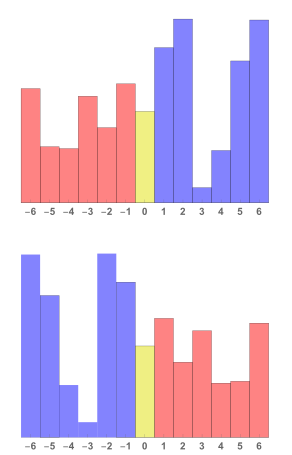
\includegraphics[width=\textwidth]{HL1dLattRefl0}
  \\ (even)
  \end{center}\end{minipage}
\qquad
  \begin{minipage}[b]{0.40\textwidth}\begin{center}
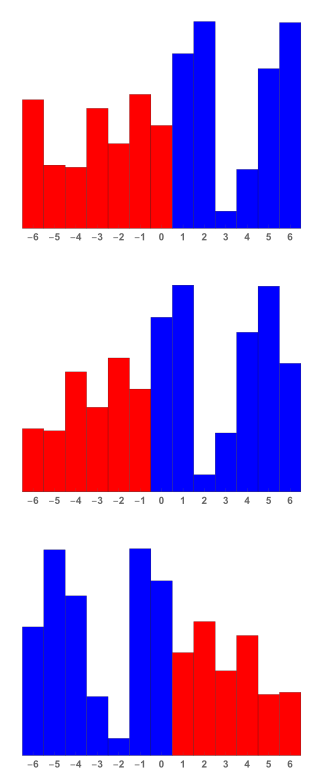
\includegraphics[width=\textwidth]{HL1dLattRefl1}
  \\ (odd)
  \end{center} \end{minipage}
  \end{center}
  \caption{\label{fig:HL1dLattRefl}
(Color online)~~~
There are two classes %\refeq{DinftyClassRefl}
of {\lattstate} reflections,
even \refeq{1dLattRefl0} and odd \refeq{1dLattRefl1}.
% :
% even, across a lattice site, and odd, across the mid-point between
% a pair of adjacent lattice sites.
    (Even)
reflection $\Refl$ exchanges (blue
$\ssp_j$) $\leftrightarrow$  (red $\ssp_{-j}$) %, $j>0$,
while leaving the yellow
field $\sitebox{\ssp_0}$ at lattice site ${0}$ fixed.
    (Odd)
reflection $\Refl_1=\Refl\shift$ swaps the
`blues' and the `reds' by a lattice
translation $\Xx\to\shift\Xx$, followed by a reflection $\Refl$. The
result is a reflection across the midpoint of the [01] interval,  marked
`|'.
See \reffig{LC21FieldConfig}\,(b) for the notation.
% Horizontal: lattice sites $j\in\integers$. Vertical: lattice site
% fields $\ssp_j$, labeled by their values before the reflection.
}
\end{figure}
%%%%%%%%%%%%%%%%%%%%%%%%%%%%%%%%%%%%%%%%%%%%%%%%%%%%%%%%%%%%%%%


\paragraph{Even class.}
Take $\Refl=\Refl_0$ as a representative of all even reflections
$\Refl_{2m}$,  and act on a {\lattstate} \refeq{1dLattStat}:
\bea
\Xx &=&
\cdots {\ssp}_{-3} {\ssp}_{-2}\,{\ssp}_{-1}\,
       {\ssp}_0\,
      {\ssp}_{1} {\ssp}_{2} {\ssp}_{3} {\ssp}_{4}  \cdots
\continue
\Refl\Xx &=&
\cdots  {\ssp}_{5} {\ssp}_{4} {\ssp}_{3} {\ssp}_{2} {\ssp}_{1}
       \sitebox{{\ssp}_0}\,
      {\ssp}_{-1} {\ssp}_{-2} {\ssp}_{-3}  \cdots
\,,
\label{1dLattRefl0}
\eea
with
\(
\sitebox{{\ssp}_0}
\)
indicating that the field at the lattice site $0$ is
unchanged by the reflection, see \reffig{fig:HL1dLattRefl}\,(even).

\paragraph{Odd class.}
 Take $\Refl_1$ as a representative of all odd reflections
$\Refl_{2m+1}$.
The result is:
\bea
\Xx &=& ~~~~\,
\cdots {\ssp}_{-3} {\ssp}_{-2} {\ssp}_{-1}
       \,{\underline {\ssp}}{}_0\,\,
      {\ssp}_{1} {\ssp}_{2} {\ssp}_{3} {\ssp}_{4}  \cdots
\continue
\shift\Xx &=& ~\,
\cdots {\ssp}_{-3} {\ssp}_{-2} {\ssp}_{-1}
       {\ssp}_0\,{\underline {\ssp}}{}_{1}\,\,
       {\ssp}_{2} {\ssp}_{3} {\ssp}_{4}  {\ssp}_{5} \cdots
\continue
\Refl_1\Xx =
\Refl\shift\Xx &=& ~~~~
\cdots  {\ssp}_{6} {\ssp}_{5} {\ssp}_{4} {\ssp}_{3} {\ssp}_{2} \,
      {\underline {\ssp}}{}_{1} | \, {\ssp}_0
      {\ssp}_{-1} {\ssp}_{-2} {\ssp}_{-3} \cdots
\,,
\label{1dLattRefl1}
\eea
where ${\underline {\ssp}}{}_{j}$ indicates the field value at the
lattice site $0$, and
\(
|
\)
indicates a reflection across midpoint
between lattice sites $0$ and $1$, see \reffig{fig:HL1dLattRefl}\,(odd).

More generally, one can say that the index $k$ in the
`translate-reflection' \refeq{Refl_k} operation
\(\Refl_{k} =\Refl\shift_k\)
advances the reflection point by $k/2$ steps, and then reflects
across it.
    \PC{2021-08-17} {
    Before publication, fine tune \reffig{fig:HL1dLattRefl}
    using LaTex, as in  \reffig{fig:1dLattRefl}.
    }

If you do not find the two kinds of reflections intuitive, the
distinction becomes crystal clear once you have a look at the
smallest Bravais lattices,
lattices of periods 3 and 4, \reffig{fig:D3D4}.

%%%%%%%%%%%%%%%%%%%%%%%%%%%%%%%%%%%%%%%%%%%%%%%%%%%%%%%%%%%%%%%%%%%%%%%%%%
\subsection{Symmetries of a system and of its solutions}
\label{s:1dSubLattSymms}

What's the deal about classes?
A `class' is a refinement of our intuitive
notion that ``rotations are rotations, and translations are
translations.''
Translated into a more familiar language,
conjugation \refeq{conjugate} is central
to all of physics: a `law' $f(\Xx)$ is invariant if it
retains its form in all symmetry related coordinate frames,
\beq
f(\Xx)  =  \LieEl^{-1} f(\LieEl\,\Xx)
\,,
\label{dscr:L-inv}
\eeq
where $\LieEl$ is a representation  of group
element $\LieEl\in \Group$.
If this holds, we say that $\Group$ is the \emph{symmetry} of the system.

For example, the `temporal Bernoulli' defining equation
\refeq{1stepDiffEq}  retains its form under conjugation by any
$\Cn{\infty}$  translation \refeq{C_infty},
\beq
\shift_i({s}\ssp_{\zeit} - \ssp_{\zeit+1})\shift_i^{-1}
= ({s}\ssp_{\zeit+i} - \ssp_{\zeit+i+1})\shift_i^{-1}
= {s}\ssp_{\zeit} - \ssp_{\zeit+1}
\,,
\ee{invBern}
while the Euler–Lagrange second-order difference equations
\refeq{LC21:1dTempFT}, `{\templatt}', `{\henlatt}', and `temporal
{$\phi^4$} theory' defining equations \refeq{LC21:1dTemplatt},
\refeq{LC21:1dHenlatt} and \refeq{LC21:1dPhi4} retain their form also
under any  $\Dn{\infty}$ reflection,
    \PC{2021-08-22} {
    This is not quite right, one does not `conjugate' a vector $\ssp_j$.
    Not sure how to elegantly deal with $\ssp_{-\zeit}^k$ term. Could
    have defined actions, but that does not work for the Bernoulli
    \refeq{invBern}.
    }
\beq
\Refl_i(
  -\ssp_{\zeit+1} + \,{g}\,V'(\ssp_{\zeit})-\ssp_{\zeit-1}
         )\Refl_i^{-1}
= -\ssp_{-\zeit+1} + \,{g}\,V'(\ssp_{-\zeit}) -\ssp_{-\zeit-1}
\,.
\ee{invPhi4}


%%%%%%%%%%%%%%%%%%%%%%%%%%%%%%%%%%%%%%%%%%%%%%%%%%%%%
\begin{figure} \begin{center}
  \begin{minipage}[b]{0.33\textwidth}\begin{center}
{(1)}~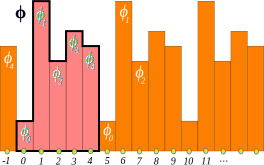
\includegraphics[width=\textwidth]{1dLatStatC_5_0}
\\
{($\shift_1$)}~\includegraphics[width=\textwidth]{1dLatStatC_5_1}
\\
{($\shift_2$)}~\includegraphics[width=\textwidth]{1dLatStatC_5_2}
\\
{($\shift_3$)}~\includegraphics[width=\textwidth]{1dLatStatC_5_3}
\\
{($\shift_4$)}~\includegraphics[width=\textwidth]{1dLatStatC_5_4}
  \end{center}\end{minipage}
\qquad\quad
  \begin{minipage}[b]{0.33\textwidth}\begin{center}
{($\Refl$)}~\includegraphics[width=\textwidth]{1dLatStatC_5_s0}
\\
{($\Refl_1$)}~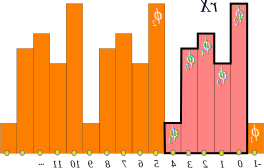
\includegraphics[width=\textwidth]{1dLatStatC_5_s1}
\\
{($\Refl_2$)}~\includegraphics[width=\textwidth]{1dLatStatC_5_s2}
\\
{($\Refl_3$)}~\includegraphics[width=\textwidth]{1dLatStatC_5_s3}
\\
{($\Refl_4$)}~\includegraphics[width=\textwidth]{1dLatStatC_5_s4}

  \end{center} \end{minipage}
  \end{center}
  \caption{\label{fig:1dLatStatC_5}
(Color online)~~~
%Horizontal circles: \lattice\ lattice sites labelled by $\zeit\in\integers$.
%Vertical: the value of field $\ssp_\zeit$, plotted as a bar centred at
%lattice site $\zeit$.
(1)
A Bravais cell $\mathbf{a}$ with
{\lattstate}
% \refeq{1dLattStatC_n}
\(\Xx=\cycle{\ssp_0 \ssp_1 \ssp_2 \ssp_3 \ssp_4}\)
with no reflection symmetry, outlined in bold, invariant under the
translation group $H_{5}$.
Its \Cn{\infty} orbit are the $\cl{}=5$ distinct {\lattstate}s (1) to
($\shift_4$), obtained by all of the $\Cn{5}$ translations.
Its \Dn{\infty}-orbit are $2\cl{}=10$ distinct {\lattstate}s,
5 translations (1) to ($\shift_4$)
and
5 translate-reflections ($\Refl$) to ($\Refl_4$), obtained by
all of the $\Dn{5}$ actions.
See \reffig{LC21FieldConfig}\,(b) for the notation.
Continued in \reffig{fig:symmLattStates}.
          }
\end{figure}
%%%%%%%%%%%%%%%%%%%%%%%%%%%%%%%%%%%%%%%%%%%%%%%%%%%%%

Given that $\Group$ is the {symmetry} of the system does not mean that
$\Group$ is also the symmetry of its solutions, or what we here call {\em
\lattstate}s.
They can satisfy
all of system's symmetries, a subgroup of them, or have no symmetry at
all.
For example, a generic {\lattstate} \refeq{1dLattStat} sketched in
\reffig{fig:HL1dLattRefl} has no symmetry beyond the identity, so its
symmetry group is the trivial subgroup $\{e\}$; any translation
$\shift_j$ or reflection $\Refl_k$ maps it into a different, distinct
{\lattstate}, as shown in \reffig{fig:1dLatStatC_5}.
At the other extreme, the constant {\lattstate}
$\ssp_j=\ssp$ is invariant under any translation or reflections - its
symmetry group is the full \Group, the symmetry of the system. In
between, there are {\lattstate}s whose symmetry is any subgroup of
$\Group$.

%%%%%%%%%%%%%%%%%%%%%%%%%%%%%%%%%%%%%%%%%%%%%%%%%%%%%%%%
\subsection{What are `{\lattstate}s'? Orbits?}
\label{s:LattStates}

Remember, for evolution-in-time, every period-\cl{}\ periodic point is a
fixed point of the \cl{}th iterate of the 1 time-step map. In the lattice
formulation, the totality of finite-period {\lattstate}s is the \emph{set
of fixed points} of all  $H_{\mathbf{a}}$ and  $H_{\mathbf{a},k}$
subgroups of $\Dn{\infty}$.

You can visualize a {\lattstate} invariant under (`fixed by') subgroup
$H_{\mathbf{a},k}$ as a tiling of the lattice $\integers$ by a
{\lattstate} tile of length \cl{}, symmetric under reflection $\Refl_k$,
see \reffig{fig:symmLattStates}\,(b-c).

    \begin{quote}
Definition: {\em
{\em Orbit} or \emph{$\Group$-orbit} of a {\lattstate} $\Xx$ is the
set of all {\lattstate}s
\beq
    \pS_\Xx = \{\LieEl\,\Xx \mid \LieEl \in {\Group}\}
\ee{GroupOrbDisc}
into which $\Xx$ is mapped under the action of group $\Group$.
We label the orbit $\pS_\Xx$ by any {\lattstate} $\Xx$ belonging to
it.
            }
    \end{quote}
As an example, the $\Dn{\infty}$ orbit of the period-5 {\lattstate}
% \refeq{1dLattStatC_n}
% \(\cycle{\ssp_0 \ssp_1 \ssp_2 \ssp_3 \ssp_4}\)
is shown in \reffig{fig:1dLatStatC_5}.
    \PC{2021-09-05} {
    This "maximal subgroup" does not seem to me to be defined here.
    Clean up!
    }
    \begin{quote}
Definition: Symmetry of a solution.
{\em
We shall refer to the maximal subgroup $\Group_\Xx \subseteq  \Group$ of
actions on {\lattstate}s within the orbit $\pS_\Xx$, which leave
the orbit invariant, as the \emph{symmetry}
$\Group_\Xx$ of the orbit $\pS_\Xx$,
\beq
\Group_\Xx =
   \{ \LieEl \in \Group_\Xx \mid \LieEl \Xx \in \pS_\Xx
   %,\,    \LieEl \ssp \neq \ssp  \mbox{ for } \LieEl \neq e
   \}
\,.
\ee{LC21:stabilSet}
}
    \end{quote}
An orbit $\pS_\Xx$ is $\Group_\Xx$-{\em symmetric}
({\em symmetric}, {\em set-wise symmetric}, {\em self-dual})
if the action of elements of $\Group_\Xx$ on
the set of {\lattstate}s $\pS_\Xx$ reproduces the orbit.
%
% \item[2021-07-28 Predrag]
% Rather than Lind's nebulous `index'\rf{Lind96}, for $|\Group/{H}|$ in
% \refeq{Ryu17eq:1.3}
    \begin{quote}
Definition: Multiplicity
{\em
of orbit $\pS_\Xx$ is given by
}
\beq
m_\Xx=|\Group|/|\Group_{\Xx}|
\,.
\ee{GroupOrbMult}
    \end{quote}
(See \toChaosBook{section*.166} {p.~166}.)



\bigskip

And now, a pleasant surprise, obvious upon an inspection of
\reffigs{fig:1dLatStatC_5}{fig:symmLattStates}: what happens
in the Bravais cell, stays in the Bravais cell.
Even though
the lattices \lattice, $\lattice_{\mathbf{a}}$ are infinite,
and their symmetries
$\Dn{\infty}$, $H_{\mathbf{a}}$, $H_{\mathbf{a},k}$ are
\emph{infinite} groups, the Bravais {\lattstate}s'
\emph{orbits} are \emph{finite}, described by the finite group
permutations of the infinite lattice curled up into a Bravais cell periodic
$\cl{}$-site ring.


%\subsection{Finite groups}
%\label{s:1dmnFntPer}


%%%%%%%%%%%%%%%%%%%%%%%%%%%%%%%%%%%%%%%%%%%%%%%%%%%%%%%%%%%%%%%%%%
% PC 2021-08-05:  from ChaosBook book/figs/D3.tex, D3.tex
\begin{figure} \begin{center}
  \begin{minipage}[b]{0.32\textwidth}\begin{center}
  \setlength{\unitlength}{1.00\textwidth}
  \begin{picture}(1,1.12469246)%
    \setlength\tabcolsep{0pt}%
    \put(0,0){\includegraphics[width=\unitlength,page=1]{D3}}%
    \put(0.23496893,0.6474626){\color[rgb]{0.1372549,0.12156863,0.1254902}\makebox(0,0)[lt]{\smash{$\shift$}}}%
    \put(0,0){\includegraphics[width=\unitlength,page=2]{D3}}%
    \put(0.34167143,0.39068967){\color[rgb]{0.1372549,0.12156863,0.1254902}\makebox(0,0)[lt]{\smash{$\shift_2$}}}%
    \put(0.05464421,0.6373038){\color[rgb]{0.1372549,0.12156863,0.1254902}\makebox(0,0)[lt]{\smash{$\Refl$}}}%
    \put(0.67969793,0.84532127){\color[rgb]{0.1372549,0.12156863,0.1254902}\makebox(0,0)[lt]{\smash{$\Refl_1$}}}%
    \put(0.44996833,0.19132446){\color[rgb]{0.1372549,0.12156863,0.1254902}\makebox(0,0)[lt]{\smash{$\Refl_2$}}}%
    \put(0,0){\includegraphics[width=\unitlength,page=3]{D3}}%
    \put(0.6357866,0.31003627){\color[rgb]{0,0,0}\makebox(0,0)[lt]{\smash{$\pSRed$}}}%
    \put(0.81616715,0.52920775){\color[rgb]{1,1,1}\makebox(0,0)[lt]{\smash{{\Large 0}}}}%
    \put(0.12429459,0.92867118){\color[rgb]{1,1,1}\makebox(0,0)[lt]{\smash{{\Large 1}}}}%
    \put(0.12402384,0.13559257){\color[rgb]{1,1,1}\makebox(0,0)[lt]{\smash{{\Large 2}}}}%
    \put(0,0){\includegraphics[width=\unitlength,page=4]{D3}}%
  \end{picture} \\ $(o)$
  \end{center}\end{minipage}
\qquad
  \begin{minipage}[b]{0.39\textwidth}\begin{center}
  \setlength{\unitlength}{1.00\textwidth}
  \begin{picture}(1,0.94270725)%
    \setlength\tabcolsep{0pt}%
    \put(0,0){\includegraphics[width=\unitlength,page=1]{D4}}%
    \put(0.11589164,0.70318699){\color[rgb]{1,1,1}\makebox(0,0)[lt]{\smash{{\Large 2}}}}%
    \put(0.11465857,0.11853823){\color[rgb]{1,1,1}\makebox(0,0)[lt]{\smash{{\Large 3
    }}}}%
    \put(0,0){\includegraphics[width=\unitlength,page=2]{D4}}%
    \put(0.69662672,0.11848457){\color[rgb]{1,1,1}\makebox(0,0)[lt]{\smash{{\Large 0}}}}%
    \put(0.69785979,0.70163221){\color[rgb]{1,1,1}\makebox(0,0)[lt]{\smash{{\Large 1}}}}%
    \put(0.48887673,0.58974203){\color[rgb]{0.1372549,0.12156863,0.1254902}\makebox(0,0)[lt]{\smash{$\shift_1$}}}%
    \put(0,0){\includegraphics[width=\unitlength,page=3]{D4}}%
    \put(0.24073374,0.49925981){\color[rgb]{0.1372549,0.12156863,0.1254902}\makebox(0,0)[lt]{\smash{$\shift_2$}}}%
    \put(0.33991763,0.28480816){\color[rgb]{0.1372549,0.12156863,0.1254902}\makebox(0,0)[lt]{\smash{$\shift_3$}}}%
    \put(0.95378545,0.34914366){\color[rgb]{0.1372549,0.12156863,0.1254902}\makebox(0,0)[lt]{\smash{$\Refl_1$}}}%
    \put(0.87112523,0.73973783){\color[rgb]{0.1372549,0.12156863,0.1254902}\makebox(0,0)[lt]{\smash{$\Refl_2$}}}%
    \put(0.50562029,0.87631462){\color[rgb]{0.1372549,0.12156863,0.1254902}\makebox(0,0)[lt]{\smash{$\Refl_3$}}}%
    \put(0.11826698,0.87765494){\color[rgb]{0.1372549,0.12156863,0.1254902}\makebox(0,0)[lt]{\smash{$\Refl$}}}%
    \put(0,0){\includegraphics[width=\unitlength,page=4]{D4}}%
  \end{picture}  \\ $(e)$
  \end{center} \end{minipage}
  \end{center}
  \caption{\label{fig:D3D4}
% Dihedral group \Dn{3}: \Dn{4}:
Translational and rotational symmetries of
    $(o)$
an equilateral triangle,  $\cl{}=3$ lattice sites;
    $(e)$
a square,                  $\cl{}=4$ lattice sites.
The $\cl{}$ rotations $\shift_j$ and the $\cl{}$ translate-reflect
$\Refl_k$ (elements of dihedral group \Dn{\cl{}} \refeq{DnElements},
even reflection axes dashed, odd reflections full line)
overly an $\cl{}$-sided regular polygon onto itself. They
also tile it with  the $2\cl{}$ copies $\pSRed_\ell$ of the fundamental
domain, indicated by the shaded wedge.
}
\end{figure}
%%%%%%%%%%%%%%%%%%%%%%%%%%%%%%%%%%%%%%%%%%%%%%%%%%%%%%%%%%%%%%%

Indeed, to grasp everything one needs to know about translations
$\shift_j$ (for regular polygons, `rotations'),
and
reflections $\Refl_k$,
it suffices to understand the symmetries of
an equilateral triangle (dihedral group \Dn{3})
and
a square (dihedral group \Dn{4}), depicted in \reffig{fig:D3D4}.
It is clear by inspection that an $\cl{}$-sided regular polygon has
$\cl{}$-fold translational symmetry and $\cl{}$ reflection symmetry axes.
The group of such symmetries is the finite dihedral group
\beq
\Dn{\cl{}} = \{1,\Refl,\shift,\Refl_{1},\shift_{2},\Refl_{2},\
           \cdots,
           \shift_{\cl{}-1},\Refl_{\cl{}-1}\}
%\,,
\ee{DnElements}
of order $2\cl{}$.
A half of its elements are the $\cl{}$ cyclic group \Cn{n} translations
$\shift_{j}$.
% 2\pi/n,2\cdot2\pi/n,\cdots$,
The other half are the $\cl{}$ reflections $\Refl_k$, one for the
reflection across each symmetry axis.
The group multiplication table is the same as the $\Dn{\infty}$
\refeq{eq:DinftyMultTab}, but with all subscripts mod $\cl{}$.
%
As in \refeq{DinftyInversion},
conjugation by any reflection reverses the direction of translation
\beq
   \Refl_i\shift_j\Refl_{-i} =  \shift_{\cl{}-j}
\,,\qquad 0<j<\cl{}
\,,
\ee{D_nInversion}now mod $\cl{}$,
so every translation pairs up with the equal counter-translation to form
a 2-element class \refeq{DinftyClassShift}. %$\{\shift_j,\shift_{\cl{}-j}\}$.

The distinction between the classes of even and odd reflections
\refeq{DinftyClassRefl} is visually self-evident by inspection of
\reffig{fig:D3D4}:
the symmetry axes either connect opposite lattice sites, or bisect the
edges, or both, if $\cl{}$ is odd (a triangle, for example).
One can say that the index $k$ in the
`translate-reflection' \refeq{Refl_k} operation
\(
\Refl_{k} %=\Refl\shift_k\,.
\) advances the reflection point by $k$ 1/2 steps, and then reflects
across it.

For a polygon with an \emph{odd} number of
lattice sites (a triangle, for example), we see by contemplating the
triangle of \reffig{fig:D3D4},  as well as by taking  mod $\cl{}$ of the
conjugation relation \refeq{D_nConj}, that
% for  $\cl{}$ odd, the
all reflections are in the same conjugacy class $\{\Refl_{j}\}$:
 there is no splitting into odd and even cases, in
contrast to the infinite lattice case \refeq{DinftyClassRefl}.

For a polygon with an \emph{even} number of lattice sites (a square, for
example), one must distinguish
the `long' axes that connect lattice sites (we label them by even numbers
$0,2,\cdots$)
from
the `short' symmetry axes that bisect opposite edges (labelled by odd
numbers $1,3,\cdots$).
%
The corresponding reflections belong to
different \Dn{\cl{}} (subclasses of
\refeq{DinftyClassRefl}),
\bea
\mbox{even reflections}
    &&\quad
\{\Refl,\Refl_{2},\Refl_{4},\cdots,\Refl_{\cl{}/2}\}
    \continue
\mbox{odd reflections}
    &&\quad
\{\Refl_{1},\Refl_{3},\cdots,\Refl_{\cl{}/2+1}\}
\,.
\label{DnClassRefl}
\eea

%%%%%%%%%%%%%%%%%%%%%%%%%%%%%%%%%%%%%%%%%%%%%%%%%%%%%%%%
\subsection{Symmetries of {\lattstate}s}
\label{s:LattStateSyms}


%%%%%%%%%%%%%%%%%%%%%%%%%%%%%%%%%%%%%%%%%%%%%%%%%%%%%
\begin{figure}
  \centering
{$(n)$}
\includegraphics[width=0.40\textwidth]{HL1dLatticeStateBar1}\quad
{$(o)$}
\includegraphics[width=0.40\textwidth]{HL1dLatticeStateBar2}
\\ %~~~
{$(ee)$}
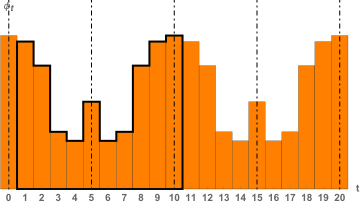
\includegraphics[width=0.40\textwidth]{HL1dLatticeStateBar4}\quad
{$(eo)$}
\includegraphics[width=0.40\textwidth]{HL1dLatticeStateBar3}

  \caption{\label{fig:symmLattStates}
(Color online)~~~
A Bravais {\lattstate} \Xx\ has one of the
4 possible symmetries, illustrated by:
$(n)$ {\em No reflection symmetry:}
    an $H_{5}$ invariant period-5 {\lattstate} \refeq{reflSymNo}. For its
    \Group-orbit, see \reffig{fig:1dLatStatC_5}.
$(o)$ {\em Odd period, reflection-symmetric:}
    an $H_{9,8}$ invariant period-9 {\lattstate} \refeq{reflSymOdd},
    %PC 2021-08-21 checked
    reflection symmetric over the lattice sites interval [8-9]  midpoint
    and over the lattice site~4.
$(ee)$ {\em Even period, even reflection-symmetric:}
    an $H_{10,0}$  invariant period-10 {\lattstate} \refeq{reflSymEvens0},
    reflection symmetric over lattice sites 0 and 5.
$(eo)$ {\em Even period, odd reflection-symmetric:}
    an $H_{10,9}$  invariant period-10 {\lattstate} \refeq{reflSymEvens1},
    reflection symmetric over the [4-5] and [9-10] interval midpoints.
Horizontal: lattice sites labelled by $\zeit\in\integers$.
Vertical: value of field $\ssp_\zeit$, plotted as a bar centred at
lattice site $\zeit$.
Even reflection axes dashed, odd reflections full line.
          }
\end{figure}
%%%%%%%%%%%%%%%%%%%%%%%%%%%%%%%%%%%%%%%%%%%%%%%%%%%%%

A Bravais {\lattstate} \Xx\ has one of the
four symmetries:

\bea
    && \mbox{ no reflection symmetry }
    \continue
(n) \quad &&
\cycle{\ssp_0 \ssp_1 \ssp_2 \ssp_3 \cdots \ssp_{\cl{}-1}}
\label{reflSymNo} \\ % the same as {1dLattStatC_n}
    &&
\mbox{ multiplicity } m_\Xx=2\cl{}
    \nnu %\,,
\eea
{\lattstate} invariant under the translation group
$H_{\cl{}}$.
Its \Group-orbit, generated by all actions of \Dn{\infty},
results  in  $2\cl{}$ distinct,  \Dn{\cl{}} related {\lattstate}s.
This is illustrated by the $H_{5}$-invariant {\lattstate} \Xx\ of
\reffig{fig:1dLatStatC_5}. %{fig:symmLattStates}\,$(n)$.
Its \Dn{5} orbit are $2\cl{}=10$ {\lattstate}s, 5  translations
and 5 translate-reflections.
    \PC{2021-08-20} {
    Merge \reffig{fig:symmLattStates}\,$(n)$ with
    \emph{1dLatStatC\_5\_0x3.svg}.
    }

Next, the reflection-symmetric {\lattstate}s.
As illustrated in \reffigs{fig:HL1dLattRefl}{fig:D3D4},
there are two classes \refeq{DinftyClassRefl} of {\lattstate} reflections:
even, across a lattice site, and
odd, across the mid-point between a pair of adjacent lattice sites.
However, as is evident by inspection of \reffig{fig:D3D4}, curling up the
lattice {\lattice} into a Bravais cell periodic $\cl{}$-site ring
implies that an axis cuts the ring twice, and
constrains the possible reflection points to three configurations:

\bea
    && \mbox{ odd period } \cl{}=2m+1
    \continue
(o) \quad &&
\cycle{\sitebox{\ssp_0} \ssp_1 \ssp_2 \cdots \ssp_{m}|\ssp_{m}\cdots \ssp_2 \ssp_1}
\label{reflSymOdd} \\
    &&
\mbox{ multiplicity } m_\Xx=\cl{}
    \nnu %\,,
\eea
{\lattstate} invariant under the dihedral group $H_{\cl{},k}$,
illustrated by the $H_{9,8}$ invariant {\lattstate} \Xx\
of \reffig{fig:symmLattStates}\,$(o)$.
% as well as by the triangle of \reffig{fig:D3D4}\,(1)).
\bea
    && \mbox{ even period } \cl{}=2m+2\,, \mbox{ even reflection } k
    \continue
(ee) \quad &&
\cycle{\sitebox{\ssp_0} \ssp_1 \ssp_2 \cdots \ssp_{m}
        \sitebox{\ssp_{m+1}} \ssp_{m} \cdots \ssp_2 \ssp_1}
\label{reflSymEvens0} \\
    &&
\mbox{ multiplicity } m_\Xx=\cl{}/2
    \nnu %\,,
\eea
{\lattstate} invariant under the dihedral group $H_{\cl{},k}$,
$k$ even,
illustrated by the $H_{10,0}$ invariant {\lattstate} \Xx\
of \reffig{fig:symmLattStates}\,$(ee)$.
\bea
    && \mbox{ even period } \cl{}=2m\,, \mbox{ odd reflection } k
    \continue
(eo) \quad &&
\cycle{\ssp_1 \ssp_2 \ssp_3 \cdots \ssp_{m}| \ssp_{m}\cdots \ssp_2 \ssp_1|}
\label{reflSymEvens1} \\
    &&
\mbox{ multiplicity } m_\Xx=\cl{}/2
    \nnu %\,,
\eea
{\lattstate} invariant under the dihedral group $H_{\cl{},k}$,
$k$ odd,
illustrated by the $H_{10,9}$ invariant {\lattstate} \Xx\
of \reffig{fig:symmLattStates}\,$(eo)$.

For long periods $\cl{}$, almost all orbits are of no-symmetry type
\refeq{reflSymNo}.
So why do we care about the symmetric orbits so much? The reason is that
the \po\ expansions are dominated by the short orbits, and many, if not
the most of those are reflection-symmetric.

The {\lattstate} {symmetry} $\Group_\Xx$ \refeq{LC21:stabilSet} of the
above $(o)$--$(eo)$ reflection-symmetric {\lattstate}s \Xx\ is the reflection
group $\Dn{1}=\{1,\Refl_k\}$, but we will spare the reader the
group-theorist's cosets and group quotients. For us, this symmetry means
two things:
\begin{itemize}
  \item[(1)]
The \Dn{\infty} orbits of reflection-symmetric {\lattstate}s contain only
translations, as any reflection amounts to a cyclic group
\Cn{\cl{}} translation.
(Try reflecting a  {\lattstate} in \reffig{fig:symmLattStates}\,(b-d)
over any lattice site or mid-interval.)
  \item[(2)]
The prime {\lattstate} is a `half' of the Bravais cell,
give or take some boundary sites, the length ${m}$ orbit,
\beq
\tilde{\Xx}      = \ssp_1 \ssp_2 \ssp_3 \cdots \ssp_{m}
\,.
\ee{primeLattStat}


\end{itemize}
Reflection breaks the translational invariance, and how one reconstructs
the period-$\cl{}$ orbit from this length-$m$ \brick\ is a bit tricky. To
develop intuition about that, it is helpful to have a look at
explicit matrix
representations of $\Dn{\cl{}}$ operations.

%%%%%%%%%%%%%%%%%%%%%%%%%%%%%%%%%%%%%%%%%%%%%%%%%%%%%%%%%%%%%%%%%%%%%%%%%%
\subsection{Permutation representation}
\label{sect:permReps}

A {\lattstate} {\Xx} over a Bravais cell $\mathbf{a}$ can be assembled
into an $\cl{}$\dmn\ vector whose components are lattice site fields
\beq
\transp{\Xx} = (\ssp_0,\ssp_1,\ssp_2,\ssp_3,\cdots,\ssp_{\cl{}-1})
\,,
\ee{1dLattStatVec}
with the first field in such vector placed at the lattice site 0, the
second at the lattice site 1, and so on. Matrices that reshuffle the
components of such vectors form the {\em permutation representation} of a
finite group \Group, which gives us a different and helpful
perspective on the three kinds of symmetric solutions of the preceding
section.

The permutation representation of 1-step lattice translation $\shift$
acts on a Bravais {\lattstate} by the off-diagonal
$[\cl{}\!\times\!\cl{}]$ matrix \refeq{hopMatrix}. This is a cyclic
\Cn{\cl{}} permutation that translates the {\lattstate} $\Xx$
"for\-ward-in-time" by one site,
\[
\transp{(\shift\Xx)}=(\ssp_1,\ssp_2,\cdots,\ssp_{\cl{}-1},\ssp_0)
\,.
\]
A permutation representation of a \Dn{\cl{}} translate-reflect operation
is essentially an anti-diagonal matrix that reverses the order of site
fields, up to a cyclic permutation
\[
\transp{(\Refl_k\Xx)}=(\ssp_{\cl{}-1},\cdots,\ssp_2,\ssp_1,\ssp_0)
\,.
\]
Symmetries of triangles and squares, \reffig{fig:D3D4}, help us make this
precise.

%     \item[2021-03-09 Han]
\emph{Odd period}:
In odd dimensions, the $\cl{}$ translate-reflect matrices of \Dn{\cl{}} are
related by translations \refeq{D_nConj}.
For example, for a period-3 {\lattstate}
without symmetry
\(
\transp{\Xx} = (\ssp_0,\ssp_1,\ssp_2)
\,,
\)
they are
\[
\Refl=
\left(
\begin{array}{ccc}
 1 & 0 & 0 \\
 0 & 0 & 1 \\
 0 & 1 & 0
\end{array}
\right)
    \,,\quad
{\Refl_1}=
\left(
\begin{array}{ccc}
 0 & 1 & 0 \\
 1 & 0 & 0 \\
 0 & 0 & 1
\end{array}
\right)
    \,,\quad
\Refl_2=
\left(
\begin{array}{ccc}
 0 & 0 & 1 \\
 0 & 1 & 0 \\
 1 & 0 & 0
\end{array}
\right)
\,.
\]
In agreement with \refeq{reflSymOdd}, \reffig{fig:D3D4}\,$(o)$ and
\reffig{fig:symmLattStates}\,$(o)$, reflections keep one lattice site fixed
(for each permutation matrix $\Refl_k$ there is only one `1' on the
diagonal), swap the rest.

Next consider a period-5 reflection symmetric {\lattstate}s tiles the infinite lattice
\lattice\ with a reflection-fixed $\sitebox{\ssp_0}$, and a length-2
{\brick} $(\ssp_1,\ssp_2)$,
\beq
\Xx =
\cdots \ssp_2 \ssp_1 \sitebox{\ssp_0} \ssp_1 \ssp_2 |
      \ssp_2 \ssp_1 \sitebox{\ssp_0} \ssp_1 \ssp_2 |\cdots
\,.
\ee{symmCycD5}
\Dn{5} permutation representation of reflections of a pentagon, illustrates that
fixpoints {\Xx} of $\Refl_{k}$ are cyclicly related:
\bea
\Refl\Xx &=&
\left(
\begin{array}{ccccc}
 1 & 0 & 0 & 0 & 0 \\
 0 & 0 & 0 & 0 & 1 \\
 0 & 0 & 0 & 1 & 0 \\
 0 & 0 & 1 & 0 & 0 \\
 0 & 1 & 0 & 0 & 0
\end{array}
\right)
\left(\begin{array}{c}
 \sitebox{\ssp_0}\cr
 \ssp_1\cr
 \ssp_2\cr
 \ssp_2\cr
 \ssp_1\cr
\end{array}\right)
=
\left(\begin{array}{c}
 \sitebox{\ssp_0}\cr
 \ssp_1\cr
 \ssp_2\cr
 \ssp_2\cr
 \ssp_1\cr
\end{array}\right)
        \continue
\Refl_{4}(\shift_{-2}\Xx )
     &=&
\left(
\begin{array}{ccccc}
 0 & 0 & 0 & 0 & 1 \\
 0 & 0 & 0 & 1 & 0 \\
 0 & 0 & 1 & 0 & 0 \\
 0 & 1 & 0 & 0 & 0\\
 1 & 0 & 0 & 0 & 0
\end{array}
\right)
\left(\begin{array}{c}
 \ssp_2\cr
 \ssp_1\cr
 \sitebox{\ssp_0}\cr
 \ssp_1\cr
 \ssp_2\cr
\end{array}\right)
=
\left(\begin{array}{c}
 \ssp_2\cr
 \ssp_1\cr
 \sitebox{\ssp_0}\cr
 \ssp_1\cr
 \ssp_2\cr
\end{array}\right)
\,.
\label{symmCycD5Refl}
\eea

The symmetry conditions are the Bravais lattice site 5-periodicity
mod 5, and the even reflection across
$\sitebox{\ssp_0}$:
\beq
\ssp_{i} = \ssp_{i+5}
    \,, \quad
\ssp_{-i} = \ssp_{i}
\,.
\ee{symmCycD5bcs}
A {\lattstate} satisfies
the defining equation \refeq{LC21:1dTempFT} %{catMapNewt}
\beq
- \ssp_{\zeit-1}  +  V'(\ssp_{\zeit}) - \ssp_{\zeit+1}
    =
\Ssym{\zeit}
\,,
\ee{LC21:1dTempFTa} %{catMapHL}
on the period-5 Bravais cell,
\bea
    V'(\ssp_{0}) - 2 \ssp_1 &=& m_0 \continue
-\ssp_0 +V'(\ssp_{1}) -\ssp_2 &=& m_1 \continue
-\ssp_1 +V'(\ssp_{2}) -\ssp_2 &=& m_2 \continue
-\ssp_1 +V'(\ssp_{2}) -\ssp_2 &=& m_2 \continue
-\ssp_0 +V'(\ssp_{1}) -\ssp_2 &=& m_1
\label{symmCycD5eqs5} % from {HLsymmCycD5eqs}
\eea
where we have used \refeq{symmCycD5bcs}.
The result is a symmetry reduced {\jacobianOrb}, with
rows modified by the \bcs,
\bea
    V'(\ssp_{0}) - 2 \ssp_1 &=& m_0 \continue
-\ssp_0 +V'(\ssp_{1}) -\ssp_2 &=& m_1 \continue
-\ssp_1 +V'(\ssp_{2}) -\ssp_2 &=& m_2
\label{symmCycD5eqs} % from {HLsymmCycD5eqs}
\eea
with a 3\dmn\ {\jacobianOrb} \refeq{jMorb1dFT}
\bea
\jMorb_+ &=&
\left(\begin{array}{ccc}
{s}_0 & -2 & 0 \\
 -1 & {s}_1 & -1 \\
 0 & -1 & {s}_2-1
\end{array}\right)
\,,
\label{OrbJacobianD5} % from {HLOrbJacobianD5}
\eea
At this point we have to abandon the detailed discussion of the four
kinds of symmetry reduced {\jacobianOrbs}: the message is that for any
reflection-symmetric Bravais cell the cyclic translational symmetry is
broken, and one has to impose the correct $\sitebox{\ssp_0}$ and odd $|$
reflection \bcs\ to define the {\jacobianOrb} for the \emph{prime} orbit.

%%%%%%%%%%%%%%%%%%%%%%%%%%%%%%%%%%%%%%%%%%%%%%%%%%%%%%%%%%%%%%%%%%%%%%%%%%
\subsection{Reciprocal lattice}
\label{sect:DnReciprLatt}


%%%%%%%%%%%%%%%%%%%%%%%%%%%%%%%%%%%%%%%%%%%%%%%%%%%
\begin{figure}
  \centering
              \begin{minipage}[c]{0.4\textwidth}\begin{center}
\includegraphics[width=1.0\textwidth]{HLCatmapD3a}\\(a)
            \end{center}\end{minipage}
            \begin{minipage}[c]{0.4\textwidth}\begin{center}
\includegraphics[width=1.0\textwidth]{HLCatmapD3b}\\(b)
            \end{center}\end{minipage}
  \caption{\label{fig:HLCatmapD3}
Period-3 {\lattstate}s of the $s=3$ \templatt, plotted in the $\Dn{3}$
permutation irreps subspaces $A_0+E$. In contrast with the
\Cn{\cl{}} complex irreps (see the \Cn{3} example
\reffig{fig:BernC3}), the 2\dmn\ irrep $E\in\reals^2$ is real.
In the subspace of the $E$ irrep,
{\lattstate}s that are related by cyclic permutations are connected by blue lines.
The 2 big triangles are a single \Dn{3} 6-{\lattstate}s orbit, what for
\Cn{3} is a pair of 3-{\lattstate}s orbits without time reversal symmetry.
The remaining 3 smaller triangles are 3 time-reversal symmetric orbits;
the pair in the middle is presumably related by the
 $\Dn{1}: S\ssp_i = 1-\ssp_i$ invariance specific to
the \templatt, a symmetry not yet taken into account. The state in
the center is the fixed point.
Red dashed lines are the reflection axes of the $\Dn{3}$ group. There are 4 states
on each reflection axis.
}
\end{figure}
%%%%%%%%%%%%%%%%%%%%%%%%%%%%%%%%%%%%%%%%%%%%%%%%%%%

When we use the similarity transformation to diagonalize the permutation
representation, the {\lattstate}s are transformed into the subspaces of
the irreps. The example of period-3 {\lattstate}s of \templatt\ with
$s=3$ is shown in \reffig{fig:HLCatmapD3}. The permutation representation
is block diagonalized by basis vectors: $e_0=1/\sqrt{3}(1,1,1)$,
$e_1=\sqrt{2/3}(\cos(2\pi/3),\cos(4\pi/3),1)$ and
$e_2=\sqrt{2/3}(\sin(2\pi/3),\sin(4\pi/3),0)$. The basis vector $e_0$
spans the subspace of the 1\dmn\ irrep $A_0$. Basis vectors $e_1$ and
$e_2$ span the subspace of the 2\dmn\ irrep $E$.

Period-3 {\lattstate}s of cat map with $s=3$ are mapped into the subspace
of the irreps $A_0$ and $E$ in \reffig{fig:HLCatmapD3}.
The irrep $A_0$ is the symmetric 1\dmn\ irrep, so in the subspace of $A_0$ the components
of {\lattstate}s are invariant under the action of the $\Dn{3}$ group.
In the 2\dmn\ subspace of the irrep $E$, the shift operator $\shift$ rotates the
{\lattstate}s clockwise by $2\pi/3$, while the reflection operator $\Refl$ reflects the {\lattstate}s
over the axis passing through the origin and pointing toward $(\cos(2\pi/3),\sin(2\pi/3))$.
In \reffig{fig:HLCatmapD3}
{\lattstate}s that are related by shifts are connected by blue lines.
The red dashed lines are reflection axis of the reflection operators.
The 2 big triangles in \reffig{fig:HLCatmapD3} subspace of $E$ are lattice states
that belong to 2 orbits which are related by time reflection. The remaining 3 triangles
are lattice states from 3 orbits which are invariant under time reflection.

If the space of the field configuration has \Dn{\cl{}} symmetry,
the subspace of the 2\dmn\ irrep $E_1$ can be divided
into $2\cl{}$ copies by the irrep. One can choose the fundamental domain to be the region
with polar angle between 0 and $\pi/\cl{}$, assuming that the horizontal axis is one of the
reflection axis of the irrep $E_1$. Each orbit only appears once in the fundamental domain,
as shown in \reffig{fig:HLCatmapD3}. Note that the two orbits related by
the time reflection are considered one orbit of the dihedral group.

If, in addition, the law is time-reversal (or time-inversion) invariant,
the symmetry includes time-reflection, ie, it is dihedral group \Dn{n}
with 2$\cl{}$ elements, so the reciprocal lattice should be a half of the
above 1/$\cl{}$ sliver of a $\cl{}$-gon, and irreps are now either 1 or 2
dimensional. Even $\cl{}$ is different from odd $\cl{}$, and solutions either appear
in pairs, or are self dual under reflection in 3 different ways.

Due to the time
reversal, all $k={2\pi}/{5}$ irrep states are the same as the
$k={4\pi}/{5}$ irrep states.


\subsubsection{Fundamental domain}
What happens when {\lattstate}s appear on the boundary of the fundamental domain?
There are two possible situations. The first situation is that the {\lattstate} belongs to an
orbit with multiplicity less than the order of the symmetry group. For example,
in \reffig{fig:HLCatmapD3} subspace of $E$, there are 3 points in the fundamental domain
with polar angle equal to 0 or $\pi/3$. These 3 points are representative {\lattstate}s of orbits
with time reflection symmetry. The multiplicities of these orbits are 3 instead of 6.

The second situation is that the multiplicity of
the orbit of the {\lattstate} is equal to the order of the symmetry group
but the component in the subspace is 0. For example,
\[
\Xx = \frac{1}{104} (17, 51, 49, 43, 25, 75)
\]
is a period-6 {\lattstate} of the temporal Bernoulli
\refeq{LC21:1dBernLatt} with $s=3$. Using the discrete Fourier transform
this {\lattstate} becomes:
\[
\cssp =
\left(\frac{5}{2 \sqrt{6}},0,\frac{-5-3 i \sqrt{3}}{13
   \sqrt{6}},-\frac{\sqrt{3}}{4\sqrt{2}},\frac{-5+3 i \sqrt{3}}{13 \sqrt{6}},0\right) \,.
\]
This is a period-6 {\lattstate}. It belongs to an orbit that
contains 6 different {\lattstate}s. The $k=1$ component of this lattice
state is 0, which is on the boundary of the fundamental domain. To put this kind of
{\lattstate}s into the fundamental domain one needs to divide other subspaces.
For this lattice state the $k=2$ and $k=3$ components are not 0. The irreps divide
the $k=2$ subspace into 3 copies and the $k=3$ subspace into 2 copies. One way to
choose the fundamental domain in these subspaces is: the argument of the component
in the $k=1$ subspace is $0\leq\arg(\cssp_{1})<\pi/3$; if the $k=1$ component
is 0, the arguments of the components
in the $k=2$ and $k=3$ subspaces are $0\leq\arg(\cssp_{2})<2\pi/3{}$ and
$0\leq\arg(\cssp_{3})<\pi$. Each orbit is guaranteed to visit this fundamental
domain exactly once.

    \ifboyscout\clearpage\fi
% siminos/reversal/Lind1d.tex      pdflatex LC21; bibtex LC21
% temporary:  siminos/spatiotemp/chapter/LC21Lind1d.tex
% $Author: predrag $ $Date: 2021-12-20 23:24:25 -0500 (Mon, 20 Dec 2021) $

% Predrag 2021-08-08: shared with siminos/reversal/LC21.tex

%%%%%%%%%%%%%%%%%%%%%%%%%%%%%%%%%%%%%%%%%%%%%%%%%%%%%%%%%%%%%%%%%%%%%%%%%%
\section{Lind zeta function}
\label{sect:LC21Lind1d}

\Poincare\rf{poincare} was the first to  recognize the fundamental role
{\po}s play in shaping ergodic dynamics. The first problem that one then
needs to address is the problem of counting {\po}s%
\rf{ArtMaz65,ChAnPi85,brucks,Lutzky88,Lutzky93,BLMS91,XH94,
CheLou97,BriPer05,CBcount}, starting with 1950's
\HREF{https://en.wikipedia.org/wiki/Pekka_Myrberg} {Myrberg}
investigations of {\po}s of quadratic maps, in what was arguably the
first application of computers to
dynamics\rf{Myrberg58a,Myrberg58b,Myrberg59,Myrberg62,Myrberg63}.
Such orbit counts are most elegantly encoded by \emph{topological zeta
functions}.

For a discrete time dynamical system
\(
\ssp_{\zeit+1}=\flow{}{\ssp_{\zeit}}
\,,\)
period-$\cl{}$ solutions (in present context, the period-$\cl{}$ Bravais
cell {\lattstate}s) are \emph{fixed point}s of the $\cl{}$th iterate map
$\map^\cl{}$.
While the symmetry of a time-invariant dynamical `law' $\map$ is
the {infinite cyclic group} \Cn{\infty},
the group of all temporal lattice translations, for a period-$\cl{}$
solution the symmetry is $\cl{}$-steps translation subgroup $H_{\cl{}}$.

This observation motivates definition of a general group-theoretic
\emph{fixed-points counting} generating  function that relates the number
of {\lattstate}s to the number of prime orbits for any \statesp\ map
\(
\map : \pS \to \pS
\)
with a symmetry group $\Group$, a counting function that applies equally
well to multi\dmn\ lattice field theories\rf{CL18} as to the 1\dmn\
theories considered here.

Let $\Group$ be a group whose action
$\alpha: \Group \times \pS \to \pS$
permutes elements of a set $\pS$.
The Lind zeta function\rf{Lind96} is defined as
\beq
\zeta_{Lind}(t) =
\exp \left( \sum_{H} \;
            \frac{N_{H}}{|\Group/{H}|}t^{|\Group/H|}
      \right)
\,,
\ee{LindZeta} % was {LindZeta}
where the sum is over all subgroups $H$ of $\Group$
of multiplicity $|G/H| < \infty$, and $N_{H}$ is the number of states
in $\pS$ invariant under action of (\ie, fixed points of) subgroup $H$,
\beq
N_{H} =
   |\{\Xx \in \pS : \mbox{ all } h \in H \quad \alpha(h,\Xx) = \Xx\}|
\,.
\ee{LindN_H} % was {LC21Ryu17eq:1.3A}
The multiplicity factor $|\Group/{H}|$ is best explained by working out a
few examples.

In the lattice field theory setting, $\pS$ is the set of all
{\lattstate}s.
For 1\dmn\ lattice field theories, the group $\Group$ is either the
{infinite cyclic group}  \Cn{\infty} of all lattice translations \refeq{C_infty},
or
the {infinite dihedral group} $\Dn{\infty}$  of all translations and
reflections \refeq{LC21D_infty}.
Their finite-multiplicity subgroups $H$ are,
respectively, infinite translation subgroups $H_{\mathbf{a}}$
\refeq{H(n)subgroup}, or $H_{\mathbf{a}}$ and infinite dihedral subgroups
$H_{\mathbf{a},k}$ \refeq{H(n,k)subgroup}.

\subsection{Artin-Mazur zeta function}
\label{sect:ArtinMazur}

Assume that the symmetry group of a given discrete time dynamical system
is the group of temporal lattice translations \Cn{\infty}, \ie, that the
defining law of dynamics is time invariant. 1\dmn\ infinite translation
subgroup $H_{\mathbf{a}}$ \refeq{H(n)subgroup} leaves {Bravais cell} of
{period} \cl{} \refeq{1DBravLatt} invariant, so the sum over $H$ in
\refeq{LindZeta} can be replaced by the sum over periods $\cl{}$, with
$N_\cl{}$ the number of {\lattstate}s of period $\cl{}$. For \Cn{\infty}
subgroups (contemplate the \Cn{\infty} column of
\reffig{fig:1dLatStatC_5}) %\,(1)-($\shift_4$)
the multiplicity is
\beq
|\Cn{\infty}/H_\cl{}|=\cl{}
\,.
\ee{CinfHnMult}
The Lind zeta function
\refeq{LindZeta} now takes form of the Artin-Mazur zeta
func\-tion\rf{ArtMaz65,CBcount}
\beq
\zeta_{\mbox{\footnotesize AM}}(z) =
     \exp\left(\sum_{\cl{}=1}^\infty
\frac{N_\cl{}}{\cl{}} z^\cl{}
         \right)
\,,
\ee{AMzeta}
which, from group-theoretic perspective, is the statement that the law
governing the dynamical system is time invariant.

In what sense is $\zeta_{\mbox{\footnotesize AM}}(z)$ a {\lattstate}
count generating  function? Given the $\zeta_{\mbox{\footnotesize
AM}}(z)$, the number of periodic points of period $\cl{}$ is given by its
logarithmic derivative (see
\HREF{http://chaosbook.org/chapters/ChaosBook.pdf\#section.18.7}
{ChaosBook}\rf{CBcount})
\beq
\sum_{\cl{}=1}N_\cl{} z^\cl{}
    = \frac{1}{\zeta_{\mbox{\footnotesize AM}}}
            \,z\frac{d}{dz} \zeta_{\mbox{\footnotesize AM}}
\,.
\ee{zetatop-N}
Let us evaluate $\zeta_{\mbox{\footnotesize AM}}$ for scalar lattice
field theories studied here.

\paragraph{Bernoulli.}
The number of Bernoulli system period-\cl{} {\lattstate}s is given in
\refeq{noPerPtsBm}, so
\bea
\zetatop(z)
 =  \exp \left(-\sum_{\cl{}=1}^\infty
\frac{{s}^\cl{} - 1}{\cl{}}z^\cl{}
         \right)
 =
\frac{1 -  {s}z}{1 - z}
\,.
\label{BernZeta}
\eea
The numerator $(1 - {s}z)$ says that a Bernoulli system is a full
shift\rf{CBcount}: there are $s$ fundamental {\lattstate}s, in this case
fixed points $\{\ssp_0,\ssp_1,\cdots,\ssp_{s-1}\}$, and every other
{\lattstate} is built from their concatenations and repeats. The
denominator $(1 - z)$ compensates for the single overcounted
{\lattstate}, the fixed point $\ssp_{{s}-1}=\ssp_{0}$ $(\mbox{mod}\;1)$
of \reffig{fig:BernPart} and its repeats. If the stretching factor
${s}=\beta$ is not an integer, the map \refeq{n-tuplingMap} is called the
`$\beta$-transformation'. For its Artin-Mazur zeta function see
\refref{FlLaPo94}.

\paragraph{\tempLatt.}
The number of \templatt\ period-\cl{} {\lattstate}s is given in
\refeq{1stepDiffSolu} into the Artin-Mazur zeta \refeq{AMzeta}, so
Isola\rf{Isola90} obtains
\bea
\zetatop(z)
 =  \exp \left(-\sum_{\cl{}=1}^\infty
\frac{\ExpaEig^\cl{} + \ExpaEig^{-\cl{}} - 2}{\cl{}} z^\cl{}
         \right)
 =
\frac{1 - s z + z^2}
     {(1 - z)^2}
\,.
\label{Isola90-13}
\eea
Conversely, given the \tzeta, the generating function for the number of
temporal {\lattstate}s of period $\cl{}$ is given by the logarithmic
derivative \refeq{zetatop-N},
\bea
\sum_{{n}=0}^\infty N_{n} z^{n}
    & = & \frac{2-{s}z}{1 - s z + z^2}-\frac{2}{1 - z}
    \continue
& = & (s-2)\left[z + ({s}+2) z^2 + ({s}+1)^2 z^3 \right.
    \ceq
      \left.\qquad\quad
      +\,({s}+2)\,{s}^2 z^4 + (s^2+ s-1)^2 z^5  +  \cdots\right]
\,,
\label{1stChebGenF}
\eea
which is indeed the generating function for $T_{\cl{}}(s/2)$, the
{Chebyshev polynomial of the first kind} \refeq{POsChebyshev}.
Why Chebyshev? Essentially because $T_k(x)$ are also
defined by a 3-term recurrence:
\bea
T_0(x) &=& 1\,,\quad
T_1(x)=x \,,
    \continue
T_k(x)  &=&  2x T_{k-1}(x) - T_{k-2}(x)
\quad \mbox{for } k \geq 2
\,.
\label{Cheb1stRecurr} %{Rangarajan17:TkRecurr}
\eea

\paragraph{\Henlatt.}
The problem of counting orbits for the {\HenonMap} was addressed
already in 1979
pioneering work by Sim{\'o}\rf{Simo79}.
For the complete horseshoe, ${a}=6$ {\HenonMap} repeller
there are $2^\cl{}$
period-$\cl{}$ {\lattstate}s, so
\bea
\zetatop(z)
 =  \exp \left(-\sum_{\cl{}=1}^\infty
\frac{2^\cl{}}{\cl{}} z^\cl{}
         \right)
\,=\,
1- 2z
\,.
\label{HenonZeta}
\eea
The numbers of the shortest period {\lattstate}s and prime orbits are
listed in \reftab{tab:LC21HamHenon}.

%%%%%%%%%%%%%%%%%%%%%%%%%%%%%%%%%%%%%%%%%%%%%%%%%%%%
\begin{table}
\begin{tabular}{c|rrrrr|rrrrr|rrrrr}
$\cl{}$ &  1 &  2 &  3 &  4 &  5 &
       6 &  7 &  8 &  9 & 10 &
      11 & \\%& 12 & 13 & 14 & 15 \\
\hline
$N_\cl{}$ &  2 &  4 &  8 & 16 &  32 &
       64 &  128 &  256 & 512 & 1024 &
      2048 & % \\%& 12 & 13 & 14 & 15 \\
             \rule[-1ex]{0ex}{3.5ex} \\
$M_\cl{}$ &   2 &   1 &   2 &  3 &  6 &
         9 & 18 &  30 & 56  & 99 &
       186 &  %% &     &     &
\end{tabular}
\bigskip
\caption{\label{tab:LC21HamHenon}
$N_\cl{}$ and $M_\cl{}$ are the numbers of
the period-$\cl{}$ {\lattstate}s and
orbits for the ${a}=6$ {\HenonMap}.
}
\end{table}
%%%%%%%%%%%%%%%%%%%%%%%%%%%%%%%%%%%%%%%%%%%%%%%%%%%%
%

\paragraph{{$\phi^4$} field theory.}
Essentially the same as the \henlatt, with $2\to3$ replacement in
\refeq{HenonZeta}.


\subsection{Kim-Lee-Park zeta function}
\label{sect:KiLePa}

There is a problem with the \templatt\ Artin-Mazur zeta
\refeq{Isola90-13}: it counts pairs of orbits related by time reversal as
distinct orbits, but the \templatt\ Euler–\-Lagrange equation
\refeq{catMapNewt} is manifestly time-reversal invariant, so
time-reversal pairs are physically equivalent.
If the symmetry group $\Group$ is not the maximal symmetry, Lind zeta
function erroneously counts some of the symmetry-related {\lattstate}s as
belonging to separate `prime orbits', a problem that repeatedly bedevils
the \wwwcb{} exposition of \po\ theory whenever dynamics is time-reversal
invariant.

In particular, if the symmetry group of temporal lattice of a
given dynamical system is the {infinite dihedral group} $\Dn{\infty}$,
the group of all translations and reflections\rf{KiLePa03}, \ie, the
defining law of dynamics is time and time-reversal invariant.

For the infinite translation $H_{\mathbf{a}}$ subgroup
\refeq{H(n)subgroup}
the multiplicity is (as illustrated by \reffig{fig:1dLatStatC_5})
\beq
|\Dn{\infty}/H_{\cl{}}| =  2\cl{}
\,.
\ee{HnMult}
As explained in \refsect{s:LattStateSyms}, the \Dn{\infty} orbits of
reflection-symmetric {\lattstate}s contain only translations, so the
multiplicity of each infinite dihedral subgroup $H_{\mathbf{a},k}$
\refeq{H(n,k)subgroup} is
\beq
|\Dn{\infty}/H_{\cl{},k}| = \cl{}
\,.
\ee{HnkMult}
The Lind zeta function \refeq{LindZeta} now counts separately the four
types of (a)symmetric {\lattstate}s\rf{KiLePa03} of
\refsect{s:LattStateSyms}
\beq
%\zeta_{\map,\Refl}(t) =
\zeta_{\mbox{\footnotesize KLP}}(t) =
\exp \Big(\sum_{\cl{}=1}^{\infty} \, \frac{N_{\cl{}}}{2\cl{}}t^{2\cl{}}
          +\sum_{\cl{}=1}^{\infty} \, \sum_{k=0}^{\cl{}-1}\,
                     \frac{N_{\cl{},k}}{\cl{}}t^{\cl{}} \Big)
\,.
\ee{KLPzeta}
The first sum is a square-root of the {Artin-Mazur} zeta func\-tion
\refeq{AMzeta}:
    % was {ArtMaz5} and  {Ryu17eq:2.1A}
\beq
\exp \left(\sum_{\cl{}=1}^\infty
\frac{t^{2\cl{}}}{2\cl{}} N_\cl{}
         \right)
= \sqrt{\zeta_{\mbox{\footnotesize AM}}(t^2)}
\,.
\ee{LC21Ryu17eq:2.1B}
This takes care of {\lattstate}s \refeq{reflSymNo} with no reflection
symmetry.
The number of reflection-symmetric {\lattstate}s does not depend on the
location of the reflection point $k$, only on the type of symmetry (see
the class counts \refeq{H(n,k)class} and \refeq{DnClassRefl}), so
\beq
N_{\cl{},k} =
          \left\{
            \begin{array}{ll}
\, N_{\cl{}, 0} \qquad \mbox{ if } \cl{} \mbox{ is odd} \\ %[1ex]
\, N_{\cl{}, 0} \qquad \mbox{ if } \cl{} \mbox{ and } k \mbox{ are even} \\ %[1ex]
\, N_{\cl{}, 1} \qquad \mbox{ if } \cl{} \mbox{ is even and } k \mbox{ is odd}
\,,
        \end{array}
           \right.
\ee{N_nkCount}
and the Lind zeta function takes the form
that we refer to as the Kim-Lee-Park\rf{KiLePa03} zeta function
\beq
\zeta_{\mbox{\footnotesize KLP}}(t)
    = \sqrt{\zeta_{\mbox{\footnotesize AM}}(t^2)} \; e^{h(t)},
\ee{KLPzetaFact}
where
\beq
h(t) = \sum_{m=1}^{\infty} \left\{
       N_{2m-1, 0}\,t^{2m-1}
       + \left(N_{2m,0}+N_{2m,1}\right)\,\frac{ t^{2m}}{2}
                               \right\}
\,.
\ee{KLPzetaExp}

\subsection{Euler product form of zeta function }
\label{sect:KiLePaEuler}

In 1966 Ihara\rf{Ihara66} defined the zeta function of an undirected
graph $\Gamma$ by analogy to Euler's product form of a zeta function,
\beq
\zeta_{\mbox{\footnotesize Ihara}}(z)_\Gamma =
        \prod_{[C]}\frac{1}{1-z^{|C|}}
\,,
\ee{Sato05Zeta}
where the product is over all equivalence classes of prime (non-self
retracing) loops $C$ of $\Gamma$, and $|C|$ denotes the length of $C$.
Ihara zeta functions%
\rf{Ihara66,Bass92,Pollicott01,Sato05,GuIsLa08,Terras10,RAEWH10,
Clair14,ZhXiHe15,Deitmar15,daCosta16,Saito18}
are ``graph-theoretic analogues of discrete Laplacians''\rf{Sunada13}
defined here in \refeq{LC21:Lap}. Even though
``undirected" refers to no preferential
time direction, they do not appear related to
the time-reversal, group-theoretic Kim-Lee-Park zeta function
\refeq{KLPzetaFact} derived above.

Still,  the idea that zeta function $\zeta_{\mbox{\footnotesize KLP}}(t)$
can be written as a product over prime {\orbit}s holds. The \statesp\
\pS\ of a $\Dn{\infty}$ invariant dynamical system is union of 2
subspaces:
\beq
\pS = \pS_{a} \cup \pS_{s}
\,,
\ee{pSunion2}
where $\pS_{a}$ is the set of pairs of asymmetric orbits \refeq{reflSymNo},
each element of the set a forward-in-time orbit and the time-reversed orbit,
and $\pS_{s}$ is the set of time reversal symmetric orbits, invariant under
reflections \refeqs{reflSymOdd}{reflSymEvens1}. Kim \etal\rf{KiLePa03}
show that the contribution of a single prime orbit $p$  to
the Kim-Lee-Park zeta function is:
\bea
1/\zeta_{\mbox{\footnotesize KLP}}(t)|_{p}=
          \left\{
            \begin{array}{ll}
\, 1 - t^{\cl{p}} \qquad\qquad\qquad\qquad\quad
                    \mbox{ if } p \in \pS_{a} \,, \\[1ex]
\, \sqrt{1 - t^{2\cl{p}}} \,\exp\left(-\frac{t^{\cl{p}}}{1-t^{\cl{p}}}
\right)     \qquad \mbox{ if } p \in \pS_{s}
\,,
        \end{array}
           \right.
\label{KLPzetap}
\eea
with the zeta function written as a product over prime {\orbit}s:
\beq
1/\zeta_{\mbox{\footnotesize KLP}}(t)=
\prod_{p_a\in\pS_{a}} (1 - t^{\cl{p_a}})
\prod_{p_s\in\pS_{s}} \sqrt{1 - t^{2\cl{p_s}}}
\exp\left(-\frac{t^{\cl{p_s}}}{1-t^{\cl{p_s}}}\right)
\,,
\ee{KLPzetaProd}
to be expanded as a power series in $t$.

To sumarize, the Euler product form of {\tzeta s} makes it explicit that
they count {\em prime orbits}, \ie, \emph{sets} of equivalent
{\lattstate}s related by symmetries of the problem. The remainder of this
section are numerical checks that this is indeed what {\tzeta s} do.

\subsection{Counting {Bernoulli} prime orbits}
\label{s:bernPrime}

Substituting the Bernoulli map \tzeta\ \refeq{BernZeta}
into \refeq{zetatop-N}
we obtain
% ------------------- siminos/mathematica/ ----------
% CatMaptopZeta.nb                                    2020-01-18
% Bernoulli map periodic points counting for CL18.tex
\bea
\sum_{n=1}N_n z^n
    &=&
 z+3 z^2+7 z^3+15 z^4+31 z^5+63 z^6+127 z^7
    \ceq
+255 z^8+511 z^9+ 1023z^{10} +2047 z^{11}
\cdots
\,,
\label{bernN_n-s=2}
\eea
in agreement with the {\lattstate}s count \refeq{LC21detBern}.
The number of \emph{prime} cycles of period $\cl{}$ is given recursively by
subtracting repeats of shorter prime cycles\rf{CBcount},
\beq
M_n\,=\,\frac{1}{n}\left( N_n - \sum _{d|n}^{d<n}\,d M_d \right)
\,,
\ee{primeCount}
where $d$'s are all divisors of $n$, hence
% ------------------- siminos/mathematica/ ----------
% CatMaptopZeta.nb                                    2020-01-18
% Bernoulli map periodic points counting for CL18.tex
\bea
\sum_{n=1}M_n z^n
    &=&
 z+  z^2+2 z^3+3 z^4+6 z^5+9 z^6+18 z^7
    \ceq
+30 z^8+56 z^9+99 z^{10} +186 z^{11}
\cdots
\,,
\label{bernM_n-s=2}
\eea
in agreement with the usual numbers of binary symbolic dynamics prime
cycles\rf{CBcount}.

\newpage % REMOVE
%%%%%%%%%%%%%%%%%%%%%%%%%%%%%%%%%%%%%%%%%%%%%%%%%%%%%%
\subsection{Counting \templatt\ {\lattstate}s}
\label{sect:LC21catCounts}    % derived from blogCats.tex {sect:PeriodicPsCount}

%%%%%%%%%%%%%%%%%%%%%%%%%%%%%%%%%%%%%%%%%%%%%%%%%%%%
\begin{table}
\begin{tabular}{c|rrrrr|rrrrr|rrrrr}
$n$ &  1 &  2 &  3 &  4 &  5 &
       6 &  7 &  8 &  9 & 10 &
      11 \\%& 12 & 13 & 14 & 15 \\
\hline
$N_n$ &   1 &   5 &  16 &  45 &  121 &
        320 & 841 & 2205 &5776 &15125&
       39601& %   &      &     & 1364
             \rule[-1ex]{0ex}{3.5ex} \\
$M_n$ &   1 &   2 &   5 &  10 &   24 &
         50 & 120 & 270 & 640 & 1500 &
       3600 &  %% &     &     &
\end{tabular}
\bigskip
\caption{\label{tab:catMapN_n-s=3}
Lattice states and {prime} orbit counts for the ${s}=3$ cat map
(Bird and Vivaldi\rf{BirViv}).
        }
\end{table}
%%%%%%%%%%%%%%%%%%%%%%%%%%%%%%%%%%%%%%%%%%%%%%%%%%%%

%    \item[2021-08-26 Han]
How to count the number of {\lattstate}s for \templatt?

\emph{No symmetry} {\lattstate}s \HillDet:
\[
N_\cl{} = \prod_{j=0}^{\cl{}-1} \left( s - 2\cos\frac{2\pi j}{\cl{}}\right)
\,.
\]
The products of eigenvalues for the $\Cn{\cl{}}$ discrete Fourier
case follows from \refeq{TableOfISP13952-2}:
\beq
\prod_{j=0}^{\cl{}-1} \left( s - 2\cos\frac{2\pi j}{\cl{}}\right)
= (\ExpaEig^{\cl{}/2}-\ExpaEig^{-\cl{}/2})^2
\,,
\ee{eigsProduct}
It's a square, because of the  $\Dn{\cl{}}$ symmetry.
Consider even, odd casses, use $\cos0=1$, $\cos\pi=-1$,
$\cos(-\theta)=\cos\theta$. The product over non-trivial eigenvalues is:
\bea
\cl{}=2m
     &&
M_{\cl{},0} =
 \prod_{j=1}^{m-1}\left({s}-2\cos\frac{\pi{j}}{m}\right)
      =  \frac{|\ExpaEig^{\cl{}/2}-\ExpaEig^{-\cl{}/2}|}
              {{\mu}\sqrt{{\mu}^2+4}}
\,,
\label{LC21:eigsProdEven}
\eea

\bea
\cl{}= 2m-1
     &&
M_{\cl{},1} =
 \prod_{j=1}^{m-1}\left({s}-2\cos\frac{2j\pi}{2m-1}\right)
     = \frac{|\ExpaEig^{\cl{}/2}-\ExpaEig^{-\cl{}/2}|}
              {{\mu}}
\,,
\label{LC21:eigsProdOdd}
\eea

Next, look at the \emph{symmetric} {\lattstate}s {\HillDet}s:

For odd $\cl{}=2m-1$,
\bea
N_{\cl{},1} = \prod_{j=0}^{m-1} \left(s-2\cos\frac{2\pi j}{\cl{}}\right)
={\mu}M_{\cl{},1}
\,.
\eea
For $\cl{}=2m$,
\bea
N_{\cl{},1} &=& \prod_{j=0}^{m-1} \left(s-2\cos\frac{2\pi j}{\cl{}}\right)
            \continue
N_{\cl{},0} &=& % \prod_{j=0}^{m} \left(s-2\cos\frac{2\pi j}{\cl{}}\right) =
                (s+2)\,N_{\cl{},1}
\,,
\eea
and
\bea
\frac{1}{2}\left(N_{\cl{},0}+
N_{\cl{},1} \right)
= \frac{\mu^2+5}{2}\prod_{j=0}^{m-1} \left(s-2\cos\frac{2\pi j}{\cl{}}\right)
= \frac{\mu^2+5}{2\mu}
\sqrt{\frac{\left(\ExpaEig^{\cl{}} + \ExpaEig^{-\cl{}} - 2\right)}
           {\mu^2+4}}
\,.
\eea
The number of {\lattstate}s can be written as polynomials:
For $\cl{}=2m-1$:
\bea
N_{\cl{},0} &=&
\mu\left(\ExpaEig^{\cl{}/2}-\ExpaEig^{-\cl{}/2}\right)
\continue
&=&
\mu^2\ExpaEig^{-1/2}\left(\ExpaEig^{m}-\ExpaEig^{-m+1}\right)
\,.
\eea
For $\cl{}=2m$:
\bea
\frac{1}{2}\left(N_{\cl{},0}+
N_{\cl{},1} \right)&=&
\frac{s+3}{2(\ExpaEig-\ExpaEig^{-1})}
\left(\ExpaEig^{\cl{}/2}-\ExpaEig^{-\cl{}/2}\right)
\continue
&=&
\frac{{\mu}^2+5}{2{\mu}\sqrt{{\mu}^2+4}}
\left|\ExpaEig^{m}-\ExpaEig^{-m}\right|
\,.
\eea
Now we can compute the $h(t)$ from \refeq{KLPzetaExp}
\bea
h(t) &=& \sum_{m=1}^{\infty} \left[
       N_{2m-1, 0}\,t^{2m-1}
       + \left(N_{2m,0}+N_{2m,1}\right)\,\frac{ t^{2m}}{2}
                               \right]
\continue
&=&
\mu\frac{\ExpaEig^{1/2} t}{1-\ExpaEig t^2}
-\mu\frac{\ExpaEig^{-1/2}t}{1-\ExpaEig^{-1}t^2}
\continue
&&+
\frac{\mu^2+5}{2(\ExpaEig-\ExpaEig^{-1})}\frac{\ExpaEig t^2}{1- \ExpaEig t^2}
-\frac{\mu^2+5}{2(\ExpaEig-\ExpaEig^{-1})}\frac{\ExpaEig^{-1} t^2}{1- \ExpaEig^{-1} t^2}
\,.
\eea
Using \refeq{KLPzetaFact} we have the symmetric {\lattstate}s
part of the Kim-Lee-Park zeta function. Expanding
this zeta function using \refeq{HLFlipGeneratingFunction}, we have:
\bea
- t \frac{\partial}{\partial t}(\ln e^{-h(t)}) &=&
t + 6 t^2 + 12 t^3 + 36 t^4 + 55 t^5 +144 t^6
\continue
&&+ 203 t^7 + 504 t^8 + 684 t^9
+1650 t^{10} + \dots
\,,
\eea
which is in agreement with \refeq{HLFlipGeneratingFunction}
and \reftab{tab:Bmack93Fixed}.

%%%%%%%%%%%%%%%%%%%%%%%%%%%%%%%%%%%%%%%%%%%%%%%%%%%%%%
\subsection{Counting {\lattstate}s}
\label{sect:LC21poCounts}    % derived from blogCats.tex {sect:PeriodicPsCount}


Given the {\tzeta} \refeq{KLPzeta} we can count the
number of {\lattstate}s from the generating function:
    \PC{2021-08-25}{
    We have the counts of the Bravais {\lattstate}s $N_\cl{}$,
    $N_{\cl{},k}$ already, from \refeq{N_nkCount}, so why don't we
    reverse the logic, start here, and get the zeta function
    \refeq{KLPzetaFact} by integration? Mention that this is an
    example of Lind zeta function\rf{Lind96} \refeq{LindZeta}
    without ever writing it down, so we do not have to explain it? It's a
    side issue for us, really.
    }
\beq
\frac{-t\frac{d}{dt}(1/\zeta_{\Refl}(t))}{1/\zeta_{\Refl}(t)}
= \sum_{\cl{}=1}^\infty N_\cl{}t^{2\cl{}}
+ \sum_{\cl{}=1}^\infty\sum_{k=0}^{\cl{}-1}N_{\cl{},k}t^{\cl{}}
= \sum_{m=1}^\infty a_m t^m \, ,
\ee{LC21zetatopGenerating}
where the coefficients are:
% https://tex.stackexchange.com/questions/401201/difference-between-align-and-alignedt
\beq
a_m =
\left\{
\begin{array}{ll}
\sum_{k=0}^{m-1} N_{m,k}^{\Refl}
= m N_{m,0}^{\Refl}
\,,\quad & \mbox{$m$ is odd}
 \, ,\\
N_{m/2} + \sum_{k=0}^{m-1} N_{m,k}^{\Refl}
= N_{m/2} + \frac{m}{2} \left(N_{m,0}^{\Refl} + N_{m,1}^{\Refl}\right)
\,,\quad & \mbox{$m$ is even}
\,.
 \end{array}\right.
\ee{LC21zetatopCoefficients}
Using the product formula of {\tzeta} \refeq{ZetaProd} and
the numbers of orbits with length up to 5 from the \reftab{tab:Bmack93Fixed},
we can write the {\tzeta}:
\bea
1/\zeta_{\Refl}(t) &=&
\sqrt{1-t^2} \exp\left(-\frac{t}{1-t}\right) (1-t^4) \exp\left(-\frac{2t^2}{1-t^2}\right)
\left(\sqrt{1-t^6}\right)^3 \continue
&& \exp\left(-\frac{3t^3}{1-t^3}\right)(1-t^6)(1-t^8)^3
\exp\left(-\frac{6t^4}{1-t^4}\right) \continue
&& (1-t^8)^2(1-t^{10})^5\exp\left(-\frac{10t^5}{1-t^5}\right)
(1-t^{10})^6 \dots \, .
\eea
The generating function is:
\bea
\frac{-t\frac{d}{dt}(1/\zeta_{\Refl})}{1/\zeta_{\Refl}}
=
t + 7t^2 + 12t^3 + 41t^4 + 55t^5 + \dots \, ,
\eea
which is in agreement with \refeq{LC21zetatopCoefficients}, where the $N_\cl{}$ and $N_{\cl{}}^{\Refl}$
are the $C_\cl{}$ and $SF_\cl{}$ in the \reftab{tab:Bmack93Fixed}.

We are not able to retrieve the numbers of fixed points by their symmetry groups using this {\tzeta} \refeq{KLPzeta}, unless we rewrite the {\tzeta} with two variables:
\beq
\zeta_{\Refl}(t,u) =
\exp \Big(\sum_{\cl{}=1}^{\infty} \, \frac{N_{\cl{}}}{2\cl{}}t^{2\cl{}}
          +\sum_{\cl{}=1}^{\infty} \, \sum_{k=0}^{\cl{}-1}\,
                     \frac{N_{\cl{},k}}{\cl{}}u^{\cl{}} \Big)
\,.
\ee{LC21FlipZetaTU}
Using this {\tzeta} $\zeta_{\Refl}(t,u)$ we can write two generating functions:
\beq
\frac{-t\frac{\partial}{\partial t}(1/\zeta_{\Refl}(t,u))}{1/\zeta_{\Refl}(t,u)}
= \sum_{\cl{}=1}^\infty N_\cl{}t^{2\cl{}}
\, ,
\ee{LC21zetatopGeneratingT}
and
\beq
\frac{-u\frac{\partial}{\partial u}(1/\zeta_{\Refl}(t,u))}{1/\zeta_{\Refl}(t,u)}
= \sum_{\cl{}=1}^\infty\sum_{k=0}^{\cl{}-1}N_{\cl{},k}u^{\cl{}}
\, .
\ee{LC21zetatopGeneratingU}
Using the product formula of this {\tzeta} and the numbers of orbits with length
up to 5 from the \reftab{tab:Bmack93Fixed}, the Kim-Lee-Park zeta function is:
\bea
1/\zeta_{\Refl}(t,u) &=&
\sqrt{1-t^2} \exp\left(-\frac{u}{1-u}\right) (1-t^4) \exp\left(-\frac{2u^2}{1-u^2}\right)
\left(\sqrt{1-t^6}\right)^3 \continue
&& \exp\left(-\frac{3u^3}{1-u^3}\right)(1-t^6)(1-t^8)^3
\exp\left(-\frac{6u^4}{1-u^4}\right) \continue
&& (1-t^8)^2(1-t^{10})^5\exp\left(-\frac{10u^5}{1-u^5}\right)
(1-t^{10})^6 \dots \, .
\eea
And the generating function from this {\tzeta} is:
\bea
\frac{-u\frac{\partial}{\partial u}(1/\zeta_{\Refl}(t,u))}{1/\zeta_{\Refl}(t,u)}
=
u + 6u^2 + 12u^3 + 36u^4 + 55u^5 + \dots \, ,
\label{HLFlipGeneratingFunction}
\eea
which is in agreement with \refeq{LC21zetatopGeneratingU}, where the $N_{\cl{}}^{\Refl}$ is the $SF_{\cl{}}$
in the \reftab{tab:Bmack93Fixed}.

\bigskip\bigskip
========================================================================
We have found
MacKay\rf{Bmack93} %1982 PhD thesis,
% {\em Renormalisation in Area-preserving Maps} has a
%chapter on reversible maps.
listed the periodic {\lattstate}s and orbits counts, together with
the counts of time reversal invariant {\lattstate}s and orbits.

\HL{2021-12-29}{
This will be moved to section of reflections or
Kim-Lee-Park zeta function.
}

    \PC{2021-12-24}{
Do cite in our paper(s).
MacKay had these numbers already
listed in Table 1.2.3.5.1 of his 1982 PhD thesis\rf{Bmack93}.
    }

    \ifboyscout\clearpage\fi
% siminos/reversal/summary.tex      pdflatex LC21; bibtex LC21
% temporary: siminos/spatiotemp/chapter/LC21summary.tex
% $Author: predrag $ $Date: 2021-12-24 01:25:20 -0500 (Fri, 24 Dec 2021) $

% was siminos/kittens/summary.tex  CL18

\section{Summary}
\label{s:summary}


%%%%%%%%%%%%%%%%%%%%%%%%%%%%%%%%%%%%%%%%%%%%%%%%%%%%%%%%%%%%%%%%%%%%%%%%
%   \PC{2016-11-10}{
How to think about matters {\spt}? As our intuition about motions of
fluids is so much better than about turbulent quantum field theories,
here we briefly describe recent advances in turbulence that underpin
ideas developed in this paper.

%%%% clip from siminos/cats/GHJSC16.tex 2020-11-18
While dynamics of a turbulent system might appear so complex to defy any
precise description, the laws of motion drive a spatially extended system
through a repertoire of recognizable unstable patterns (clouds, say),
each defined over a finite  {\spt} region\rf{GuBuCv17,GudorfThesis}.
The local dynamics, observed through such finite spatiotemporal windows,
can be thought of as a visitation sequence of a finite repertoire of
finite patterns.
To make predictions about such system,  one needs to know how often a
given pattern  occurs, and that is a purview of \po\ theory\rf{focusPOT}.
Early 2000's rapid progress in description of turbulence in terms of such
`{\ecs}s'\rf{KawKida01,science04,GHCW07} has since slowed down to a crawl
due to our inability to extend the theory and the computations to
spatially large or infinite computational domains\rf{WFSBC15}.

In dynamics, we have no fear of the infinite extent in time. That is \po\
theory's\rf{DasBuch} raison d'\^{e}tre; the dynamics itself describes the
infinite time strange sets by a hierarchical succession of \po s, of
longer and longer, but always finite periods (with no artificial external
periodicity imposed along the time axis). And, since 1990's we know how
to deal with both spatially and temporally infinite regions by tiling
them with {\spt}ly periodic tiles\rf{Christiansen97,FE03,GHCW07}. A time
{\po} is computed in a finite time, with period \period{}, but its
repeats ``tile'' the time axis for all times. Similarly, a {\spt}ly
periodic ``tile'' or ``\twot'' is computed on a finite spatial region
$L$, for a finite period \period{}, but its repeats in both time and
space directions tile the infinite spacetime.

These ideas open a path to determining exact solutions on \emph{spatially
infinite} regions, and many physical turbulent flows of come equipped
with $D$ spatial translational symmetries. For example, in a pipe flow at
transitional Reynolds number, the azimuthal and radial directions
(measured in viscosity length units) are compact, while the pipe length
is infinite. If the theory is recast as a $d$\dmn\ space-time theory,
\(d= D +1\,,\)
{\spt}ly translational invariant recurrent solutions are \dtors\
(and \emph{not} the $1$\dmn\ temporal \po s of the traditional {\po} theory),
and the symbolic dynamics is likewise $d$\dmn\
(rather than a 1\dmn\ temporal string of symbols).

This changes everything. Instead of studying time evolution of a chaotic
system, one now studies the repertoire of {\spt} patterns compatible with
a given PDE, or, in the discretized spacetime, partial difference
equation. There is no more \emph{time} in this vision of nonlinear
\emph{dynamics}! Instead, there is a \statesp\ of all {\spt} patterns,
and the likelihood that a given finite {\spt}ly pattern can appear, like
the mischievous grin of Cheshire cat, anywhere, anytime in the turbulent
evolution of a flow. A bold vision, but how does it work?
\\
%   } %end censored \PC{2016-11-10 Curb you enthusiasm}
%%%%%%%%%%%%%%%%%%%%%%%%%%%%%%%%%%%%%%%%%%%%%%%%%%%%%%%%%%%%%%%%%%%%%%%%

It is in the context of working out the geometry of infinite-dimensional
{\statesp}s of turbulent fields\rf{hopf48} (\emph{not} 3\dmn\ visualizations of
fluids!) that we find the lessons learned from discretized field
theories studied in this paper very helpful.
Already 1\dmn\ lattice discretization teaches us so much that it deserves
this paper by itself, with mechanics of higher dimensional Bravais lattices
reserved for the sequel\rf{CL18}.

We have learned that, in order to describe turbulence, one has to think
globally, but act locally. Turbulence is described by a catalogue of
\spt\ patterns, ({`{\lattstate}s'} in the present, discretized field
theory context; `tiles' in the PDE settings\rf{CL18,GuBuCv17}), each a
numerically exact \emph{global} solution, satisfying the
\emph{local} deterministic Euler–Lagrange equations lattice site by site.
Stripped to its essentials, the problem is to systematically enumerate
them, compute them, and determine their relative importance:

\begin{enumerate}
              \item
\emph{{\Lattstate}s.} Each solution $\Xx_c$ is a zero of
a global {\em fixed point} condition
\[
F[\Xx_c] = 0
\,.
\]
Together, they form the deterministic scaffold, the $\infty$\dmn\
\statesp\ of  \spt\ `patterns' explored by classical (or
semiclassical or stochastic) turbulence.
              \item
{\em Global stability} is given by the {\jacobianOrb}
\[
\jMorb_{ij} =\frac{\delta F[\Xx_c]_i}{\delta \ssp_j}
\,.
\]
In
field-theoretical formulation there is no evolution in time; Hill's
formulas relate the two notions of stability.
              \item
{\em {\HillDet}s} \[
\Det\jMorb
\]
determine the numbers of \spt\ orbits and the weight of each. In the
\spt\ formulation, time-periodic orbits of dynamical systems theory are
replaced by periodic $d$\dmn\ {Bravais cell} tilings ($d$-tori) of
spacetime, each weighted by the inverse of its instability, its Hill
determinant.
The weighted sum over \spt\ `patterns' leads to `chaos theory' partition
sums much like those of  the solid state, field theory and statistical
mechanics.

              \item
{\em Symmetries.} One has to use them. The reciprocal {\lattstate}s are
neatly organized by well established crystallography. In particular, from
a \spt\ field theory perspective, `time'-reversal is a purely
crystallographic notion, a reflection point space group, leading to an
symmetry quotienting of time-reversible theories and to the associated
topological zeta functions of perhaps surprising form.

              \item
{\em Zeta functions.}
If you have the zeta function $\zeta(z)$,
you have all predictions of the theory.
In contrast to conventional solid state calculations, hyperbolic
shadowing of large Bravais cells by smaller ones\rf{GutOsi15,GHJSC16}
ensures that the predictions of the theory are dominated by the smallest
cells.
            \end{enumerate}
 %\section{Conclusions}
The \reffig{fig:MNGrfig2} is a comparison between the spatial integration
of \refeq{e-MNGre12} using the compilation method I employed in
\texttt{timeperiodic.m} and the time integration of \refeq{e-MNGre3}
using the ETDRK4 numerical scheme implementation of MATLAB file
\texttt{ksint.m}. The behavior of these figures seem to exhibit similar
patterns up to a what appears to be a reflection in the time direction,
implying that there is some unaccounted symmetry. This can be seen by
what I call the ``tails" of the pattern in the middle being pointed in
opposite directions for time and space integration.

The hope for my code is to be capable of spatial integration of infinite
 extent. My results are disappointing to me to say the least, having been
  thrown for loops by what should have been insignificant details, but
  I hope to use what I've learned in terms of coding in the future.

Some possible means of improving the equations is to look for better ways to
 dealias the pseudo-spectral term or to use the same method but require it to be more rigorous (e.g. more zero-padding).

Second would be to write an integration scheme that could produce more
accurate results. My first thought is to apply the ETDRK4 schema to spatial
 integration, however, I'm not sure if this would work with a system of
 equations rather than a single PDE.

We have detailed a {\spt} formulation of turbulence
which treats all continuous dimensions with translational
invariance equally and
explains solutions as collections of {\fpo}s.

The new techniques we developed allow us
to extract small {\po}s from larger {\po}s (clipping) and build larger {\po}s
by combining smaller {\po}s (gluing).
\subsection{Numerical robustness}

While we hope to eventually apply these ideas to equations with more continuous
dimensions there are still many tough questions yet to be answered.
\section{Future work}
These methods provides a numerical foundation
with which to investigate a 2{\dmn}{\spt} symbolic dynamics.
Specifically, by gluing members of the three continuous families of {\fpo}s
we can begin to probe the grammar of the proposed {\symbolic} by looking
for admissible orbits.

The most important question is how to incorporate
continuous families into the proposed  2\dmn\ \spt\ {\symbolic}.
The existence of continuous families makes the determination of the {\symbolic} grammar
particularly difficult. One reason is because our method for
determining the grammar is ultimately an empirical process.
The admissibility of every {\po} is
dependent upon the convergence of the optimization problem, which in turn may depend on
which {\fpo} family members ares used in the construction of the initial guess.
Therefore, we can be mislead by initial guesses which do not converge to the corresponding
{\po} it shadows. In addition to being sensitive to initial guesses, the
failure to converge can also be the fault of insufficient numerical methods.
The most obvious course of action is to improve the
optimization and gluing methods, with respect to their frequency of convergence.
The former of these two improvements is fairly
straightforward; find and implement better numerical methods. This seems
to be the low hanging fruit as we have employed some of the simplest available
algorithms. Improving the gluing method is less straightforward; but there are
also many potential improvements.

The first set of gluing improvements we discuss center around the reduction of
the number of false negatives (not converging to a {\po}). We consider
the inclusion of local Galilean velocity towards this end. Historically,
when performing simulations on a single spatially periodic domain,
Galilean invariance has been invoked to constrain the mean value of
the velocity field to zero. This does not mean, however, that the \emph{local}
Galilean velocity be zero. This detail could be included in each gluing such that the
local Galilean velocity of each {\fpo} would be included as a free parameter. By
doing so we can theoretically construct better guesses by increasing the
agreement between {\fpo}s at their boundaries.

The second gluing improvement we offer is the proper usage of the {\fpo} continuous families.
In other words, instead of using three static representatives of the families
we would reference the entire family during the gluing. This could be employed to
minimize differences at the
boundaries as well as in the periods.
In a similar vein, we need to incorporate symmetries into the construction process.
This extends the freedom of choice from picking a member of a family to
picking a member of each families' group orbit. For instance, during the gluing
process one is free to choose whether to use a {\fpo} or its reflection.
In the process of probing the {\symbolic} grammar, numerical convergence is not
the only factor which is required for success. The {\po} found via optimization
must also correspond to the original {block} it was targeting. If this is not
upheld, then the result is deemed a false positive; numerical but not symbolic
convergence.


Our only method of classifying false positives is visual inspection;
obviously an inefficient method that needs to be improved.
For example, assume that a {block}
contains $N$ symbols representative of the {\defect} family. If the {\po}
which the initial guess converges to does not include the signatures of $N$
defects then we claim that it cannot be a manifestation of the original {block}.
We have tried a number of methods which
attempt to identify features of {\fpo}s via image detection
or their topological signatures via persistent homology with
no real success. A possible brute force method would be to attempt to clip
and compare subdomains with {\fpo}s. The problem with this
is the incredible number of subdomains which could be clipped; a crude
approximation is on the order of $\mathcal{(NM)^2}$. Choose a corner
of the subdomain ($N$ choices in time, $M$ in space) then identify the
dimensions of the rectangular subdomain ($N-1$ choices in time, $M-1$ in space).
Therefore this brute force method does not seem to be a realistic option.
Each of these improvements introduces a layer of complexity which
quickly compound with one another making gluing a very complex process.

The guiding principle for all of these improvements
is that they minimize the cost function residual \refeq{e-cost} by
mitigating the error at the gluing boundaries and the error due to difference
in periods. We point out that simply reducing the cost function with no consideration
towards the method is not useful. For instance,
setting $\utensor=\mathbf{0}$ reduces the residual to zero but it quite clearly not of any use.
Better metrics to gauge the merit of these additional techniques would perhaps be
the frequency of convergence to the correct {\po} symbolically (true positive rate).

Another common occurrence is the stretching of solutions in time where large swathes shadow
equilibria. The numerical description of this effect is that during the variational search
the time dimension being stretched, as evidenced by the large difference in time
period. This reduces the magnitude of the temporal tangents which
brings it close to equilibria In other words, stretching of the
variational ``rubber band'' kills any tangential variation. This process
is evidenced by numerical continuation of various solutions. For instance,
the merger tile has a maximum spatial domain size at which point the torus
essentially contracts into a relative equilibrium. This process is (numerically) irreversible;
reducing the domain size of the newly found relative equilibrium does not
bring the original merger tile back.

For our purposes a collection on the order of a thousand \twots\
was collected but this was likely overkill; as seemingly indicated by the number
of fundamental tiles.

It is of course desirable to match tiles based on their boundaries as to reduce the severity of numerical
discontinuities. A more subtle reason to access the entire family is to match the
\spt\ domain size of the neighbors. Solving the optimization problem is equivalent
to enforcing the tangent space to behave according to the governing equations.
The magnitudes of the each tangent; \spt\ derivatives, are affected by the magnitude
of the temporal and spatial domain sizes.

%What is missing:
This paper mainly sets the stage and shows the feasibility for a \spt\ theory. There
is still much more work required to advance the theory.

Not only do we lack the symbolic
dynamics to describe infinite space-time, we also describe a smart system for enumerating all
\twots.
We currently lack a systematic approach for the enumeration of all

Solving the linear system directly by computing the (pseudo) inverse
of the matrix
is only available for problems of dimension smaller than those that
occur in Navier-Stokes
computations. In fact, this method wouldn't be feasible in the larger
case at all and
would have to be replaced with an alternative; a common choice is to
use iterative
methods such as GMRES \rf{Saad1986}. Another aspect that has room for
improvement is
the choice of norm used in the cost function. There have been cases
where the
approximate \twot\ hardly changes (visually) even though the cost
 function is
decreasing from $10^{-4}$ to $10^{-14}$. The tolerance is strict
because we want
the best approximations possible; especially in regards to the
fundamental tiles
whose acquisition is detailed next.

A common criticism and source of skepticism as to these methods
is the requirement
to maintain the entire \spt\ discretization in memory. While this
 is proper cause for
concern, comparisons with other studies shows a dramatic increase
in performance.
For example, in \rf{LCC06}, the tolerance was much less strict,
 the discretization
was larger, and the numerical methods required the inversion of
large matrices.

In our case, coarse \spt\ discretizations remain viable and
because the convergence is
occurring in spectral space it is not only easier to interpolate
 points (via zero padding of
the spectrum) but also produces more accurate results than with
 finite differencing.

%%%%%%%%%%%%%%%%%%%%%%%%%%%%%%%%%%%%%%%%%%%%%%%%%%%%%%%%%%%%%%%%%%%%%%%%%%

\ack
Work of H.~L. was fully supported by the family of late G. Robinson,
Jr..
No actual cats, graduate or undergraduate %, have shown interest in, or
were harmed during this research. This paper sets up the necessary
underpinnings for the quantum field theory of \catlatt, the details of
which we leave to our % always trustworthy
friends Jon Keating and Marcos Saraceno.

%%%%%%%%%%%%%%%%%%%%%%%%%%%%%%%%%%%%%%%%%%%%%%%%%%%%%%%%%%%%%%%%%%%%%%%%%%

%    \ifboyscout
%%    \clearpage
%\bigskip\noindent
%    {\scriptsize
%To obtain a simple heading of `Appendix' use the code
%\verb"\section*{Appendix}". If it contains numbered equations, figures or
%tables the command \verb"\setcounter{section}{1}" must follow it.
%    }
%    \fi %end of the internal draft switch

%\appendix
%   \ifboyscout\clearpage\fi
%\input{appeLiangstein}

    \ifsubmission
\section*{References}
    % from ctan.org/tex-archive/biblio/bibtex/contrib/iopart-num/ :
\bibliographystyle{iopart-num}       % APS-like style for physics
\bibliography{../bibtex/siminos}
    \else
\printbibliography[
heading=bibintoc,
title={References}
				  ] %, type=online]  % if not using default "Bibliography"
    \fi

%%%%%%%%%% Submission: cut here  %%%%%%%%%%%%%%%%%%%%%%%%%%%

    \ifboyscout
%    \clearpage
%\input{censored}
%    \PCedit{ %2019-05-27
%\section{Hill's formula}
%\label{c-Hill}  % temporary, while being edited in spatiotemp/
%% siminos/spatiotemp/chapter/action.tex
% $Author: predrag $ $Date: 2021-12-24 01:25:20 -0500 (Fri, 24 Dec 2021) $

% \ifblog  Predrag 2021-06-12 gave up on this,
%          do not remember who calls it other than blogCats.tex
    \chapter{Hill's formula}
    \label{c-Hill}  % temporary, while being edited in spatiotemp/
%\renewcommand{\cl}[1]{{\ensuremath{n_{#1}}}}   % discrete length of a cycle, Predrag
\renewcommand{\shift}{\ensuremath{\ell}}

\section{An overview over ``Hill's formulas''}
\label{sect:Hill}
%\renewcommand{\cl}[1]{{\ensuremath{|#1|}}}  % the length of a periodic orbit, Ronnie
\renewcommand{\shift}{\ensuremath{d}}

\begin{quote}
A succinct  explanation of the Hill's formula:\\
If you evaluate stability of the 3-term recurrence \refeq{JiKoKr20(2)} on
a periodic lattice you get the {\jacobianOrb} $\jMorb$;
if you evaluate it by multiplying the `two-configuration representation'
matrix $\jMps$, you get the `time evolution' side of the Hill's formula.
\end{quote}

We should emphasize that, while discovered first in Lagrangian setting,
Hill's formulas are much more general, they
apply also to dissipative dynamical systems as well, see

CL18 \HREF{http://chaosbook.org/~predrag/papers/CL18.pdf\#subsection.1.5}
{sect.~1.5} {\em  Stability of an orbit vs.  its time-evolution stability}

CL18 \HREF{http://chaosbook.org/~predrag/papers/CL18.pdf\#appendix.C}
{appendix~C} {\em Spatiotemporal stability}


\refsect{LiTom17b:GenFctn} {\em Generating functions; action}
%\else  Predrag 2021-06-12 gave up on this,
%          do not remember who calls it other than blogCats.tex
%\subsection{Generating functions; action}
%\fi


\refsect{sect:HillLagr} {\em Hill's formula, Lagrangian setting}


\refsect{sect:catlattHill} {\em \catLatt\ Hill's formula}


\refsect{sect:catlattHillrel} {\em Hill's formula for \rpo s}


\refsect{sect:templattHillHan} {\em Han's \templatt\ Hill's formula}


\refsect{sect:catlattHillHan} {\em Han's  \catlatt\ Hill's formula}


\refsect{sect:catlattHillRelativeHan} {\em Han's relative-periodic Hill's formula}


\refsect{sect:HenonHillHan} {\em Han's  \HenonMap\ Hill's formula}











\section{Generating functions; action}
%\else  Predrag 2021-06-12 gave up on this,
%          do not remember who calls it other than blogCats.tex
%\subsection{Generating functions; action}
%\fi
\label{LiTom17b:GenFctn}

    \PC{2016-11-11, 2018-09-26}{
What follows is (initially)
copied from Li and Tomsovic\rf{LiTom17b}, \emph{Exact relations between
homoclinic and \po\ actions in chaotic systems} arXiv source
file, then merged with the MacKay-Meiss-Percival action
principle \refrefs{MKMP84,meiss92}.
    }
For discrete-time one-degree-of-freedom Lagrangian systems satisfying a
periodicity condition (\ie, cat map):
\beq
\genF(\coord+1, \coord'+1)=\genF(\coord, \coord')+C
\,,
\ee{MacMei83-2}
one can consider relative periodic paths (or pre-periodic paths, also called
periodic paths of type $(\shift,\cl{})$ by Mackay and Meiss\rf{MacMei83}), with
    \PC{2018-09-29} {presumably they are \rpo s, or pre-\po s, with a rational
    winding number $p/\coord$.}
\beq
\coord_{i+\cl{}}=\coord_{i}+\shift
\,.
\ee{MacMei83-3}
Every $\coord_{i}$ returns to its value after time period $\cl{}$, but shifted by
$\shift$.
Orbits satisfying \refeq{MacMei83-3} are given by stationary points of the action
\beq
\action = \sum_{i=0}^{q-1} \genF(\coord_i, \coord_{i+1})
\ee{MacMei83-4}
in the space of periodic paths of type $(\shift,\cl{})$.
For periodic paths, it suffices to consider one period, because an orbit is periodic if
and only if it is a stationary point of the action of one period in the space
of periodic paths.

If the constant $C$ (the
\HREF{https://floerhomology.wordpress.com/2015/09/14/mean-action-and-the-calabi-invariant/}
{Calabi invariant}\rf{Calabi70}) in the periodicity condition
\refeq{MacMei83-2} is zero, and the Lagrangian satisfies a convexity
condition
\beq
\genF_{12}(\coord, \coord') < 0
\,,
\ee{MacMei83-5}
where subscript $k$ refers to the derivative with respect to the $k$th
argument, then the action of periodic paths of type  $(\shift,\cl{})$ is bounded below,
so there is a minimising path. Since its action is stationary, it gives a \po\
of type  $(\shift,\cl{})$.

    \PC{2018-01-21}{Is this true?
To go from the Hamiltonian $(\ssp_{\zeit},p_{\zeit})$ phase space formulation to the
Newtonian (or Lagrangian) $(\ssp_{\zeit-1},\ssp_{\zeit})$ {\em state space}
formulation, replace $p_\zeit$  by
\(
p_\zeit = (\ssp_{\zeit} - \ssp_{\zeit-1})/\Delta\zeit \,,
\)
where $\Delta\zeit =1$.
    }
    %
For {\orbit} ${p}$  of period $\cl{p}$, the {action} of the \orbit\ is:
\beq
\label{eq:DefGenFprimePOs}
\action_{p}  \equiv \sum_{n=0}^{\cl{p}-1}\genF(\coord_{n},\coord_{n+1})\ .
\eeq
$\action_{p}$ is the generating function that maps a point along the orbit for one
(prime) period.  For the case of a fixed point $p$ of period $\cl{p}=1$,
the action is
\beq\label{eq:Definition generating function fixed points}
\action_{p}  = \genF(\coord_p,\coord_p)
\,,
\eeq
where the generating function $\genF(\coord_p,\coord_p)$ maps $\ssp_p$ into itself in one
iteration.

\section{Homoclinic and \po\ actions in chaotic systems}

    \PC{2018-09-29}{
What follows is copied from Li and Tomsovic\rf{LiTom17b}.
    }
For an aperiodic orbit $\lbrace\ssp_0\rbrace$ going through the point $\ssp_0$,
the action, evaluated as the sum over an infinity of successive mappings,
\begin{equation}
\label{eq:full orbit action in general}
\action_{\lbrace \ssp_0 \rbrace}
\equiv \lim_{N \to \infty}
\sum_{n=-N}^{N-1} \genF(\coord_{n},\coord_{n+1})
=\lim_{N \to \infty} \action_{-N,N}
\,,
\end{equation}
is not necessarily convergent. However, the MacKay-Meiss-Percival action
principle\rf{MKMP84,meiss92} can be applied to obtain well defined
action differences between pairs of orbits.  For example,
the {\em relative} {\em action}
$\Delta \action_{\lbrace h_0 \rbrace  \lbrace x \rbrace}$ between a fixed point $\ssp_p$
and its homoclinic orbit $\lbrace h_{0} \rbrace$, where $h_{\pm
\infty}\to \ssp_p$:
\begin{eqnarray}
\label{eq:relative action homoclinic}
\Delta \action_{\lbrace h_0 \rbrace  \lbrace \ssp_p \rbrace}
 &\equiv & \lim_{N \to \infty} \sum_{i=-N}^{N-1}\left[\genF(h_i,h_{i+1})-\genF(\ssp_p,\ssp_p)\right]
\nonumber \\
&=& \int\limits_{U[\ssp_p,h_{0}]}p\mathrm{d}\coord+\int\limits_{S[h_{0},\ssp_p]}p\mathrm{d}\coord
= \oint_{US[\ssp_p,h_{0}]} p\mathrm{d}\coord \nonumber \\
&=& {\cal A}^\circ_{US[\ssp_p,h_{0}]}
\end{eqnarray}
where $U[\ssp_p,h_{0}]$ is the segment of the unstable manifold from $\ssp_p$ to
$h_{0}$, and $S[h_{0},\ssp_p]$ the segment of the stable manifold from $h_0$
to $\ssp_p$.  The $\circ$ superscript on the last line indicates that the area
is interior to a path that forms a closed loop, and the subscript
indicates the path: $US[\ssp_p,h_{0}]=U[\ssp_p,h_{0}]+S[h_{0},\ssp_p]$.  The
clockwise enclosure of an area is positive, counterclockwise negative.
$\Delta \action_{\lbrace h_0 \rbrace \lbrace \ssp_p \rbrace} $ gives the
action difference between the homoclinic orbit segment $[
h_{-N},\cdots,h_{N} ]$ and the length-$(2N+1)$ fixed point orbit segment
$[ \ssp_p, \cdots, \ssp_p ]$ in the limit $N \to \infty$. In later sections, upon
specifying the symbolic code of the homoclinic orbit $\lbrace h_0 \rbrace
\Rightarrow \overline{0} \gamma \overline{0}$, we also denote $\Delta
\action_{\lbrace h_0 \rbrace  \lbrace \ssp_p \rbrace}$ alternatively as
\begin{equation}\label{eq:relative action homoclinic symbolic notation}
\Delta \action_{\lbrace h_0 \rbrace  \lbrace \ssp_p \rbrace}
= \Delta \action_{\overline{0} \gamma \overline{0},  \overline{0}}
\end{equation}
by replacing the orbits in the subscript with their symbolic codes.

%%%%%%%%%%%%%%%%%%%%%%%%%%%%%%%%%%%%%%%%%%%%%%%%%%%%%%%%%%%%%%%%%%%%%
\begin{figure}
   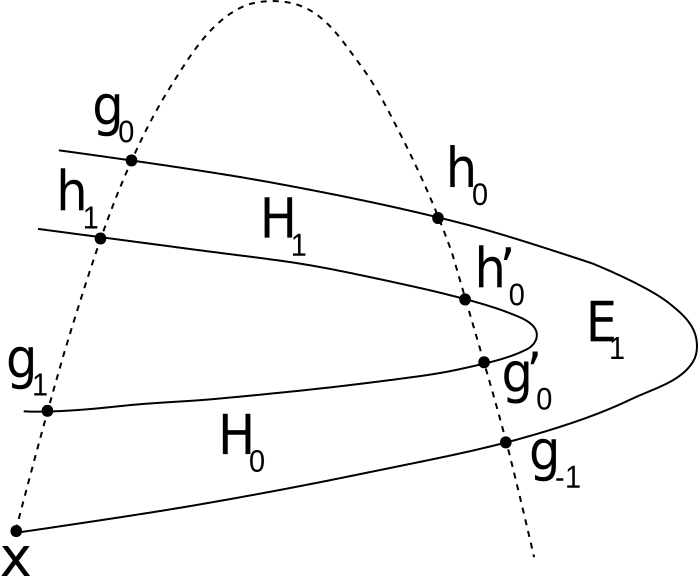
\includegraphics[width=0.5\textwidth]{LiTom17bHorseshoe2}
\caption{\label{fig:Horseshoe2}
A sketch of a partial homoclinic tangle
which forms a complete horseshoe structure. The unstable (stable)
manifold of $x$ is the solid (dashed) curve. There are two primary
homoclinic orbits $\lbrace h_0\rbrace$ and $\lbrace g_0\rbrace$.
$\cal{R}$ is the closed region bounded by loop
$\mathcal{L}_{USUS[x,g_{-1},h_0,g_0]}$.
~(From \refref{LiTom17b})
        }
\end{figure}
%%%%%%%%%%%%%%%%%%%%%%%%%%%%%%%%%%%%%%%%%%%%%%%%%%%%%%%%%%%%%%%%%%%%%

Likewise, a second important case is for the relative action between a
pair of homoclinic orbits $\lbrace h^{\prime}_0\rbrace \Rightarrow
\overline{0} \gamma^{\prime} \overline{0} $ and $\lbrace h_0\rbrace
\Rightarrow \overline{0} \gamma \overline{0}$, which results in
\begin{eqnarray}
\label{eq:homoclinic action difference}
\Delta \action_{{\lbrace h^{\prime}_0\rbrace}{\lbrace h_0\rbrace}} &\equiv & \lim_{N \to \infty} \sum_{i=-N}^{N-1}\left[ \genF(h^{\prime}_{i},h^{\prime}_{i+1}) - \genF(h_{i},h_{i+1})\right] \nonumber \\
& = & \lim_{N \to \infty} \left[ \genF(h^{\prime}_{-N},h^{\prime}_{N}) - \genF(h_{-N},h_{N}) \right] \nonumber \\
& = & \int\limits_{U[h_{0},h^\prime_{0}]}p\mathrm{d}\coord+\int\limits_{S[h^\prime_{0},h_{0}]}p\mathrm{d}\coord =  {\cal A}^\circ_{US[h_0,h^\prime_{0}]} \nonumber \\
& = & \Delta \action_{ \overline{0} \gamma^{\prime} \overline{0},  \overline{0} \gamma \overline{0} }
\end{eqnarray}
where $U[h_{0},h^\prime_{0}]$ is the segment of the unstable manifold
from $h_{0}$ to $h^\prime_{0}$, and $S[h^\prime_{0},h_{0}]$ the segment
of the stable manifold from $h^\prime_{0}$ to $h_{0}$.  Due to the fact
that the endpoints approach $\ssp_p$ forward and backward in time, one can
also write
\begin{eqnarray}
\label{eq:homoclinic action difference2}
\Delta \action_{{\lbrace h^{\prime}_0\rbrace}{\lbrace h_0\rbrace}}
& = & \lim_{N \to \infty}
\left[ \genF(h^{\prime}_{-(N+n)},h^{\prime}_{N+m}) - \genF(h_{-N},h_{N})
      \right] \nonumber \\
& & - (n+m) {\cal F}_0
\,.
\end{eqnarray}

%%%%%%%%%%%%%%%%%%%%%%%%%%%%%%%%%%%%%%%%%%%%%%%%
    \ifblog
\newpage
% siminos/spatiotemp/chapter/Hill.tex
% $Author: predrag $ $Date: 2021-12-08 23:33:01 -0500 (Wed, 08 Dec 2021) $

%\chapter{Hill's formula} %called by blogCats.tex and CL18.tex
%\label{c-Hill}  % temporary, while being edited in spatiotemp/

%\Chapter{Hill}{28jan2018}{Hill's formula}   % formatted for ChaosBook.org
%\label{c-Hill}
%\listofsections{0}

\section{Hill's formula, Lagrangian setting}
\label{sect:HillLagr}

    \PC{2016-11-11, 2018-09-26}{
The current draft of this section starts out with
excerpts from
Mackay and Meiss\rf{MacMei83}
{\em Linear stability of periodic orbits in {Lagrangian} systems},
 and
Bolotin and Treschev\rf{BolTre10} {\em Hill's formula}.
    }
%
There can be more than one minimising path. In particular,
translating one minimising path by an integer in time or space or both gives
another. This implies existence of saddle points of the action in between the
minima, with one downward direction [1-3]. They are called minimax points, and
give rise to minimax \po s of type $(\shift,\cl{})$. The statement of the existence of
at least two \po s of each type  $(\shift,\cl{})$ is known as the Poincar\'e-Birkhoff
theorem.

As a corollary, Mackay and Meiss\rf{MacMei83} rederive the old result
that when the convexity condition is satisfied, the multipliers of a
minimising orbit are a reciprocal pair of positive reals, and those of a
minimax orbit are either a complex conjugate pair on the unit circle, or
a reciprocal pair of negative reals. The result for minimising orbits was
shown by \Poincare\rf{Poinc1886} for two-degree-of-freedom
continuous-time systems, and Birkhoff [1] discusses the minimax case.

The linear stability of a \po\ is determined by its multipliers, the eigenvalues
of the derivative of the return map round the orbit. While the first variation of
the action is by definition zero for an orbit, the multipliers of a \po\ can be
related to the second variations of the action in the space of periodic paths.
This has been shown in various cases. Hill\rf{Hill86} and \Poincare\rf{Poinc1886}
derived a formula for the multipliers in the case of one-degree-of-freedom
systems of the form kinetic minus potential\rf{Hill86}, using a Fourier
representation for periodic paths. In his study of \po s of the three-body
problem, Hill obtained a formula connecting the characteristic polynomial of the
monodromy matrix of a \po\ with the infinite determinant of the Hessian of the
action functional. Mackay and Meiss\rf{MacMei83} derived a formula
\refeq{MacMei83(17)} for the multipliers of a \po\ for general discrete-time
one-degree-of-freedom systems. Bolotin and Treschev\rf{BolTre10} give two
multidimensional generalizations of Hill's formula: for discrete Lagrangian
systems (symplectic twist maps) and for continuous Lagrangian systems, and
discuss implications of symmetries and reversibility. Bountis and
Helleman\rf{Bount81} and Greene\rf{gree79} treated the case of discrete-time
one-degree-of-freedom systems with
\beq
\genF_{12}(\coord,\coord') = -1
\,.
\ee{MacMei83(6)}
Schmidt\rf{Schmidt84} determined $n$-tupling bifurcations by the criterion
that the matrix of second variations of the action
with respect to periodic paths of $n$ times the period
have a zero eigenvalue.


Mackay and Meiss\rf{MacMei83} relate the multipliers of a periodic orbit to the second variations of
the action about the orbit, and compute the {\HillDet} of the matrix
of second variations of the action in the space of periodic
paths of period $\period{}$.

Stationarity \refeq{MKMP84(3.7)} of the action for an orbit of a
discrete-time one-degree-of-freedom system implies that
\beq
\genF_2(\coord_{i-1},\coord_{i}) + \genF_1(\coord_i,\coord_{i+1}) = 0
\,.
\ee{MacMei83(7)}
Thus the tangent orbits $\delta \ssp_i$ satisfy [...]. The multipliers
\ExpaEig\ of a \po\ of period $q$ are
defined by existence of a tangent orbit satisfying [...] residue of a \po\
one can easily solve for multipliers. [... losing steam]


Mackay and Meiss\rf{MacMei83} formulas for the multipliers of minimising and
minimax orbits follow. Under the convexity condition
\refeq{MacMei83-5}, the denominator is positive. At a minimum of action
(whether local or global):
\beq
D(1) \leq 0
\,,
\ee{MacMei83-18}
so the multipliers are real and positive. At a minimax with one downward
direction:
\beq
D(1) \geq 0
\,,
\ee{MacMei83-19}
so the multipliers are on the unit circle or the negative real axis.

Residue\rf{gree79} $R$ of a \po\ $p$ of period \cl{p}
\beq
4R = \det(\matId-\jMps_p)
   = \tr(\matId-\jMps_p)
   = 2-\ExpaEig_p-1/\ExpaEig_p
\ee{MacMei83(16)}
is related to the {\HillDet} $D(\ExpaEig)$ by
what the discrete Hill's formula\rf{BolTre10}:
    \PC{2018-09-30}{See Bolotin and Treschev\rf{BolTre10} eqs.~(2.8) and (2.13)}
\beq
\det (\matId-\jMps_p) = -D(1)\left(\prod_{i=0}^{\cl{p}-1}(-\genF_{12}[i,i+1])\right)^{-1}
\,.
\ee{MacMei83(17)}
This formula was derived by Mackay and Meiss\rf{MacMei83} and
Allroth\rf{Allroth83} (Allroth eq.~(12)). It applies to general
``one-degree-of-freedom'' systems, \ie, 1D lattices with only the nearest
neighbor interactions. For a finite set of neighbors, \ie, higher\dmn\
discrete-time systems, Allroth\rf{Allroth83} has some partial results in the
context of Frenkel-Kontorova models.

$D(1)$ is the {\HillDet} of the matrix of second variations of
the action in the space of periodic paths of period q. So we have related the
multipliers of a \po\ to the second variations of the action about
the orbit.

\newpage %TEMP
\renewcommand\speriod[1]{{\ensuremath{L_{#1}}}}  %continuous spatial period
\renewcommand\period[1]{{\ensuremath{T_{#1}}}}  %continuous time period
%
\section{\catLatt\ Hill's formula}
\label{sect:catlattHill}

\begin{description}
  \item[2020-07-23 Predrag]
I have everything in place for deriving \catlatt\ (and \templatt as a special
case) Hill's formula from the elementary Kronecker product
\refeq{KroneckerProd} block matrix rules
    \begin{enumerate}
      \item multiplication \refeq{mixedProd} leads to
            shift \refeq{shiftPower} accruing correctly.
      \item {\HillDet} \refeq{wikiKron2}, \refeq{detShiftxJ};
            yields correct ln det = tr ln reduction to periodic $J_p$
      \item $\mathbf{A}\otimes\mathbf{B}$ being similar to
            $\mathbf{B}\otimes\mathbf{A}$ by \refeq{wikiKron3} explains why
            [$2\speriod{}\!\times\!2\speriod{}$] phase space is
            equivalent to the [$\speriod{}\!\times\!\speriod{}$] orbit
            stability.
    \end{enumerate}
  \item[2020-07-23 Predrag]
Next: streamline, move to CL18.tex
  \item[2020-07-27 Predrag]
Essential parts copied to CL18.tex, \emph{siminos/kittens/Hill.tex}
\end{description}

\bigskip\bigskip

The $d=2$ lattice \catlatt\ equations can be recast in a
matrix form, by rewriting the defining equations as block
matrices\rf{Dorr70,ChenM87,HuRyCo98}, constructed by the
\HREF{https://en.wikipedia.org/wiki/Kronecker_product} {Kronecker
product} $\mathbf{A}\otimes\mathbf{B}$,%
    \PC{2020-08-01}{The Zehfuss product (1858), really. The {\HillDet} is
    from 1886, though it does not look recognizably anything like out the
    {\HillDet}s... These things are
    \HREF{https://www.cs.cornell.edu/cv/ResearchPDF/KPHist.pdf}
    {everywhere!}
    }
an operation that replaces
elements of the [$n\times{n}$] matrix $\mathbf{A}$ by [$m\times{m}$]
matrix `blocks' $\mathbf{B}$, resulting in an [$mn\times mn$] block
matrix\rf{ArWeHa13,wikiKronProd}
\beq
\mathbf{A}\otimes\mathbf{B} =
\left[\begin{array}{ccc} %\begin{bmatrix}
  a_{11} \mathbf{B} & \cdots & a_{1n}\mathbf{B} \\
             \vdots & \ddots &           \vdots \\
  a_{n1} \mathbf{B} & \cdots & a_{nn} \mathbf{B}
\end{array}\right] %\end{bmatrix}
\,.
\ee{KroneckerProd}
Consider $\mathbf{A}$, $\mathbf{C}$ square matrices of size
[$n\times{n}$], and $\mathbf{B}$, $\mathbf{D}$ square matrices of size
[$m\times{m}$].
The matrix product of two block matrices is a block
matrix\rf{ArWeHa13,wikiBlockMat},
\beq
(\mathbf{A}\otimes\mathbf{B})\,(\mathbf{C}\otimes\mathbf{D})
%= (\mathbf{A}\mathbf{C})\otimes(\mathbf{B}\mathbf{D})
%  {\displaystyle (\mathbf {A} \otimes \mathbf {B} )(\mathbf {C} \otimes \mathbf {D} )
  =(\mathbf{AC})\otimes (\mathbf{BD})
  \,.
\ee{mixedProd}
The trace and the determinant of a block matrix are given by
\bea
\tr(\mathbf {A} \otimes \mathbf {B})
    &=& \tr\mathbf{A}\,\tr\mathbf{B}
    \continue
\det\left(\mathbf{A} \otimes \mathbf{B}\right)
    &=& \det\left(\mathbf{A}^{m}\right) \det\left(\mathbf{B}^{n}\right)
\,.
\label{wikiKron2}
\eea
The two [$mn\times mn$] block matrices $\mathbf{A}\otimes\mathbf{B}$ and
$\mathbf{B}\otimes\mathbf{A}$ are equivalent by a similarity
transformation
\beq
\mathbf {B} \otimes \mathbf {A}
=\transp{\mathbf {P}} \,(\mathbf {A} \otimes \mathbf {B} )\,\mathbf {P}
\,,
\ee{wikiKron3}
where $\mathbf{P}$ is permutation matrix. As $\det{\mathbf{P}}=1$,
the block matrix determinant
$\det\left(\mathbf{A}\otimes\mathbf{B}\right)
=
\det\left(\mathbf{B}\otimes\mathbf{A}\right)$
is independent of the order in which blocks are constructed.

Now, apply this formalism to a $\BravCell{\speriod{}}{\period{}}{0}$ rectangular Bravais
cell. In the Kronecker product block matrix notation
\refeq{KroneckerProd}, the \jacobianOrb\ refeq\{eq:BxAtempJ\} can be
written as a $[\speriod{}\period{}\times\speriod{}\period{}]$ block
matrix
\beq
\jMorb
=
\unit_{1} \otimes \left(\shift_{2}+\shift_{2}^{-1}\right)
-
2 {s}\,\unit_1\otimes\unit_{2}
+
\left(\shift_{1}+\shift_{1}^{-1}\right) \otimes \unit_{2}
\,,
\ee{catalattLxT}
where the \refeq{KroneckerProd} matrix $\mathbf{A}$ and identity
$\unit_1$ matrix are `spatial' [$\speriod{}\!\times\!\speriod{}$]
matrices, with blocks $\mathbf{B}$ and identity $\unit_2$ `temporal'
[$\period{}\!\times\!\period{}$] matrices, with indices `1', `2'
referring to `spatial', `temporal' lattice directions, respectively.

Our goal is to compute the {\HillDet} $|\det \jMorb|$. As we have
shown in the example refsect\{s:catLattRel3x2\},  % a CL18.tex section
this is best done directly, by computing the volume of the {\fundPip}.
    \PC{2020-07-27}{
Insert refsect\{s:catLattRel3x2\} example here?
    }

However, in classical and statistical mechanics, one often computes the
{\HillDet} using a  Hamiltonian, or `transfer matrix' formulation.
An example is the \templatt\ 3-term recurrence
\refeq{genFuncts:CatMapNewt} % in the blog
%\refeq{eq:CatMapNewt} % in CL18.tex
in the \PV\rf{PerViv} `two-configuration' cat map representation
\refeq{eq:StateSpCatMap}
%     \PC{2020-07-15}{in CL18 remove \refeq{eq:StateSpCatMap_Hill}}
\beq
 \hat{\mathbf{\ssp}}_{\zeit+1} =
      {\hat{\mathbf{\jMps}}_1}\,\hat{\mathbf{\ssp}}_\zeit - \hat{\mathsf{\Ssym{}}}_\zeit
\,,
\ee{PV2config}
with the one-time step temporal evolution [$2\!\times\!2$] {\jacobian}
matrix ${\hat{\mathbf{\jMps}}_1}$ generating a time orbit by acting on the
2\dmn\ `phase space' of successive configuration points
\beq
 {\hat{\mathbf{\jMps}}_1}
=
 \left[\begin{array}{cc}
 0 & 1 \\
 -1 & s
 \end{array} \right]
\,,\qquad
\hat{\mathbf{\ssp}}_\zeit
=
\left(
\begin{array}{c}
 \ssp_{\zeit-1}\\
 \ssp_{\zeit}
 \end{array}
 \right)
\,,\qquad
\hat{\mathsf{\Ssym{}}}_\zeit
=
    \left(
\begin{array}{c}
 0           \\
 \Ssym{\zeit}
 \end{array}
    \right)
\,,
\ee{PV2configJ}
Similarly, for the $d=2$ \catlatt\ lattice at hand, one can
recast the 5-term recurrence (XX) %\refeq{CatMap2d}
(compare with the \refeq{FGHLW74:charFunct1d})
\bea
\ssp_{n\zeit}
&=& ~~\ssp_{n\zeit}
%(- \ssp_{n+1,\zeit-1} + 2{s} \, \ssp_{n,\zeit-1} - \ssp_{n-1,\zeit-1})
%- \Ssym{n,\zeit-1}
%- \ssp_{n,\zeit-2}
    \continue
\ssp_{n,\zeit+1}
&=&  - \ssp_{n,\zeit-1}
 +(- \ssp_{n-1,\zeit} + 2{s} \, \ssp_{n\zeit} - \ssp_{n+1,\zeit})
- \Ssym{n\zeit}
%\,,
\label{CatMap2dHill}
\eea
in the `two-configuration' matrix form \refeq{PV2config} by picking the
vertical direction (indexed `2') as the `time', with temporal 1-time step {\jacobian}
[$2\speriod{}\!\times\!2\speriod{}$] block matrix
% ${\hat{\mathbf{\jMps}}_1}$
\beq
{\hat{\mathbf{\jMps}}_1}  =
 \left[\begin{array}{c|c}
{\bf 0} & \unit_1\\ \hline
-\unit_1 & {-\mathbf{\jMorb}_1}
 \end{array} \right]
\,,
\ee{PV2catlattJ}
(known as a transfer matrix in statistical
mechanics\rf{Onsager44,MonMun94}) generating a time orbit by acting on a
$2\speriod{}$\dmn\ `phase space'  lattice strip
$\hat{\mathbf{\ssp}}_\zeit$ along the `spatial' direction  (indexed `1'),
\beq
\hat{\mathbf{\ssp}}_\zeit
=
\left[\begin{array}{c}
 {\mathbf{\ssp}}_{\zeit-1}\\ \hline
 {\mathbf{\ssp}}_\zeit
 \end{array}\right]
,\quad
\hat{\mathsf{\Ssym{}}}_\zeit
=
    \left[\begin{array}{c}
    \mathbf{0}\\ \hline
 \mathbf{\Ssym{}}_{1\zeit}
 \end{array}\right]
,\qquad
\mathbf{\ssp}_\zeit
=
\left[\begin{array}{c}
 \ssp_{1\zeit}\\   \vdots\\ \ssp_{\speriod{}\zeit}
 \end{array}\right]
,\quad
\mathsf{\Ssym{}}_\zeit
=
    \left[\begin{array}{c}
 \Ssym{1\zeit}\\ \vdots\\ \Ssym{\speriod{}\zeit}
 \end{array}\right]
,
\ee{PV2catlattJ1}
where the hat $\hat{~}$~ indicates a $2\speriod{}$\dmn\
`two-configuration' state, and $\mathbf{\jMorb}_1$ is the spatial
$[\speriod{}\!\times\!\speriod{}]$ {\jacobianOrb} of  form (XX),
\beq
\mathbf{\jMorb}_1
        =
\shift_{1}^{-1} - 2s \unit_1 + \shift_{1}
\label{Hessian_Hill}
\eeq
The `two-configuration' coupled cat maps system \refeq{PV2config} is a
generalization of the Bernoulli map time evolution formulation (XX) to a
higher-dimensional spatially-coupled lattice.
Just as in the {temporal Bernoulli} condition refeq \{tempFixPoint\}, the
first order in time difference equation \refeq{PV2config} can be viewed
as a {\lattstate} fixed point condition refeq\{tempFixPoint\}, a
zeros of the function
\( %beq
F[\hat{\Xx}] = \hat{\mathbf{\jMorb}}\hat{\Xx}+\hat{\Mm} = 0
\,,
\) %\ee{tempPV2Point}
with the entire periodic \emph{{\lattstate}} $\hat{\Xx}_{\Mm}$ treated as a
single fixed \emph{point} in the
$2\speriod{}\period{}$\dmn\ unit hyper-cube, and the
$[2\speriod{}\period{}\times2\speriod{}\period{}]$  block matrix \jacobianOrb\
given either by
\beq
\hat{\mathbf{\jMorb}} =
    \hat{\unit} - {\hat{\mathbf{\jMps}}_1}\otimes\shift_2^{-1}
\,,
\ee{tempPV2conf12}
or by
\beq
\hat{\mathbf{\jMorb}}' =
    \hat{\unit} -\shift_2^{-1} \otimes {\hat{\mathbf{\jMps}}_1}
\,.
\ee{tempPV2conf21}
Here the unity $\hat{\unit}=\hat{\unit}_1\otimes\unit_{2}$ is a
[$2\speriod{}\period{}\!\times\!2\speriod{}\period{}$] block matrix, and
the time-evolution \jacobianM\ ${\hat{\mathbf{\jMps}}_1}$
\refeq{PV2catlattJ} is a [$2\speriod{}\!\times\!2\speriod{}$] matrix.

The order in which the block matrix blocks are composed does not matter,
yielding the same the {\HillDet} $\det\hat{\mathbf{\jMorb}} =
\det\hat{\mathbf{\jMorb}}'$ by \refeq{wikiKron3}.
However, written out explicitly, the two \jacobianOrbs\
\refeq{eq:orbitJPVJxS} and \refeq{eq:orbitJPVtempJ} are of a very
different form.

For example, for the $\BravCell{\speriod{}}{\period{}}{0}$  rectangular
Bravais cell, the \catlatt\ \jacobianOrb\ (XX) involves the
[$\period{}\!\times\!\period{}$] time {\shiftOp} block matrix $\shift_2$
(XX) with the one-time-step [$2\speriod{}\!\times\!2\speriod{}$]
time-evolution \jacobianM\ ${\hat{\mathbf{\jMps}}_1}$ \refeq{PV2catlattJ}
\bea
\hat{\mathbf{\jMorb}}
    &=&
\left[\begin{array}{c|c}
 \unit_{1}\otimes\unit_{2}   & -\unit_1\otimes\shift_2^{-1}             \\ \hline
 \unit_1\otimes\shift_2^{-1}& \unit_{1}\otimes\unit_{2} +\mathbf{\jMorb}_1\otimes\shift_2^{-1}
\end{array}\right]
\,,
\label{eq:orbitJPVJxS}
\eea
and for \catlatt\ \refeq{CatMap2dHill} this is a time-periodic
[$\period{}\times\period{}$]  {\shiftOp} block matrix $\shift_2$ (XX),
each block now a space-periodic [$2\speriod{}\!\times\!2\speriod{}$] matrix
${\hat{\mathbf{\jMps}}_1}$ \refeq{PV2catlattJ}.

If a block matrix is composed of four blocks,
\HREF{https://en.wikipedia.org/wiki/Block_matrix\#Block_matrix_inversion}
{its determinant} can be factorized by Schur's (1917)
formula\rf{Schur1917,wikiBlockMat}
    \index{Schur!formula}
% \refeq{det2x2blockMat***
\beq
\det\left[\begin{array}{c|c}
\mathbf{A} & \mathbf{B} \\ \hline
\mathbf{C} & \mathbf{D}
\end{array}\right]
=
\det(\mathbf{A})\,\det(\mathbf{D}-\mathbf{C}\mathbf{A}^{-1}\mathbf{B})
\,.
\ee{det2x2blockMat}
so, noting \refeq{mixedProd}, \refeq{catalattLxT} and
\refeq{Hessian_Hill}, we find that the
$[2\speriod{}\period{}\times2\speriod{}\period{}]$ `phase space'
$\det\hat{\mathbf{\jMorb}}$ defined by \refeq{eq:orbitJPVJxS} is actually
the desired {\HillDet} of
$[\speriod{}\period{}\times\speriod{}\period{}]$ \jacobianOrb\
$\mathbf{\jMorb}$,
\bea
\det\hat{\mathbf{\jMorb}}
    &=&
\det\left[\begin{array}{c|c}
 \unit_{1}\otimes\unit_{2}   & -\unit_1\otimes\shift_2^{-1}             \\ \hline
 \unit_1\otimes\shift_2^{-1}& \unit_{1}\otimes\unit_{2} +\mathbf{\jMorb}_1\otimes\shift_2^{-1}
\end{array}\right]
     \continue
     &=&
% \det(\unit_1)\,
\det\left[
       \unit_{1}\otimes\unit_{2} + \mathbf{\jMorb}_1\otimes\shift_2^{-1}
     + (\unit_1\otimes\shift_2^{-1})(\unit_{1}\otimes\unit_{2})(\unit_1\otimes\shift_2^{-1})
    \right]
     \continue
     &=&
\det\left[
       \unit_{1}\otimes\unit_{2} + \mathbf{\jMorb}_1\otimes\shift_2^{-1}
     +  \unit_1\otimes\shift_2^{-2}
    \right]
     \continue
     &=&
\det(\shift_2^{-1})\,
\det\left[
       \unit_1\otimes\shift_2^{-1}
        +(\shift_{1}^{-1} - 2s \unit_1 + \shift_{1})\otimes\unit_2
     +  \unit_1\otimes\shift_2
    \right]
     \continue
     &=&
\det \jMorb
\,,
\label{det2x2blockMat2LH}
\eea
where we have used
$\det\unit_{1}=\det\unit_{2}=\det\shift_{1}=\det\shift_{2}=1$.

Consider next \refeq{tempPV2conf21}, the equivalent way of forming of the
block matrix for the $\BravCell{\speriod{}}{\period{}}{0}$  rectangular
Bravais cell, with temporal period taken for definitiveness $\period{}=4$.
The \catlatt\ \jacobianOrb\ \refeq{tempPV2conf21} is now constructed as
the [$4\times4$] time {\shiftOp} block matrix $\shift_2$ (XX), with the
one-time-step [$2\speriod{}\!\times\!2\speriod{}$] time-evolution
\jacobianM\ ${\hat{\mathbf{\jMps}}_1}$ \refeq{PV2catlattJ} and unit
matrix $\hat{\unit}_1$ as blocks
\beq
\hat{\mathbf{\jMorb}}'
 =
\unit_2\otimes\hat{\unit}_{1} -\shift_2^{-1} \otimes {\hat{\mathbf{\jMps}}_1}
 =
\left[\begin{array}{c|c|c|c}
 \hat{\unit}_1    &  {\bf 0}   & {\bf 0}    &-{\hat{\mathbf{\jMps}}_1} \\ \hline
-{\hat{\mathbf{\jMps}}_1} &  \hat{\unit}_1   & {\bf 0}    & {\bf 0}    \\ \hline
 {\bf 0}    &-{\hat{\mathbf{\jMps}}_1} & \hat{\unit}_1    & {\bf 0}    \\ \hline
 {\bf 0}    &  {\bf 0}   &-{\hat{\mathbf{\jMps}}_1} & \hat{\unit}_1
\end{array}\right]
\,.
\label{eq:orbitJPVtempJ}
\eeq
To evaluate the {\HillDet} $\det\hat{\mathbf{\jMorb}}'$, note that from
the block-matrix multiplication rule \refeq{mixedProd} and the determinant rule \refeq{wikiKron2}
it follows that
\beq
(\shift_2^{-1}\otimes{\hat{\mathbf{\jMps}}_1})
(\shift_2^{-1}\otimes{\hat{\mathbf{\jMps}}_1})
=
\shift_2^{-2}\otimes{\hat{\mathbf{\jMps}}_1}^2
\,,\quad
(\shift_2^{-1} \otimes {\hat{\mathbf{\jMps}}_1})^k =
\shift_2^{-k} \otimes {\hat{\mathbf{\jMps}}_1}^k
\,,
\ee{shiftPower}
and
\beq
\det(\shift_2^{-1}\otimes{{\hat{\mathbf{\jMps}}_1}})
=
(\det\shift_2)^{-\speriod{}}
(\det{\hat{\mathbf{\jMps}}_1})^\period{}
=
\det\hat{\mathbf{\jMps}}_p
\,,\qquad
\hat{\mathbf{\jMps}}_p = {\hat{\mathbf{\jMps}}_1}^\period{}
\,,
\ee{detShiftxJ}
where $\hat{\mathbf{\jMps}}_p$ is the {\jacobianM} of a
temporal periodic orbit $p$.
Expand
\(
 \ln\det\hat{\mathbf{\jMorb}}'
   =
 \tr\ln\hat{\mathbf{\jMorb}}'
\)
as a series using \refeq{wikiKron2} and \refeq{shiftPower},
\beq
\tr\ln\hat{\mathbf{\jMorb}}' =
\tr\ln(\unit-\shift_2^{-1} \otimes {{\hat{\mathbf{\jMps}}_1}})
  =
-\sum_{k=1}^\infty\frac{1}{k}{\tr(\shift_2^{-k})}\,\tr{{\hat{\mathbf{\jMps}}_1}}^{k}
\,,
\ee{LnDet=TrLn_Hill}
and use
$\Tr \shift_2^k=\period{}$
if $k$ is a multiple of $\period{}$,
0 otherwise
(follows from $\shift_2^\period{}=\unit$):
\[
\ln\det(\unit-\shift_2^{-1} \otimes {{\hat{\mathbf{\jMps}}_1}})
  =
-\sum_{r=1}^\infty\frac{1}{r}\tr\hat{\mathbf{\jMps}}_p^{r}
  =
\ln\det(\hat{\unit}_{1}-\hat{\mathbf{\jMps}}_p)
\,.
\]
So for the {\catlatt} the {\jacobianOrb}  and the temporal evolution
\refeq{PV2config} stability ${{\hat{\mathbf{\jMps}}_{p}}}$ are related by
the remarkable Hill's formula
\beq
|\det\jMorb|
  =
|\det(\hat{\unit}_{1}-\hat{\mathbf{\jMps}}_p)|
\,.
\ee{detBern2n}
which expresses the  {\HillDet} of the arbitrarily large \jacobianOrb\
$\hat{\mathbf{\jMorb}}'$  in terms of a determinant of a small
[$2\speriod{}\!\times\!2\speriod{}$] time-evolution \jacobianM\
${\hat{\mathbf{\jMps}}_1}$.

{\bf Remark}                                \toCB
From \refeq{det2x2blockMat1} we have
\beq
\det {\hat{\mathbf{\jMps}}_1} =
\det
 \left[\begin{array}{cc}
{\bf 0} & \unit_1\\
-\unit_1 & {-\mathbf{\jMorb}_1 }
\end{array}
\right]
=
\det(\mathbf{\jMorb}_1)\,\det(\mathbf{\jMorb}_1^{-1}) = 1
\,,
\ee{det2x2blockMat3}
so ${\hat{\mathbf{\jMps}}_1}$ is a canonical, or phase-space volume preserving
transformation, as one expects of Hamiltonian systems.


{\bf Remark}
The reformulation of the \catlatt\ 5-term recurrence \refeq{CatMap2dHill}
as the `two-configuration' form \refeq{PV2config} is really just the
usual passage from Lagrangian to the Hamiltonian formulation, but we
chose to short-circuit it, as all that heavy general formalism is not
needed for the problem at hand.
    \PC{2020-07-15}{
Perhaps refer to \toChaosBook{section.8.1} {8.1 Hamiltonian flows}.
Mention transfer matrix formulation of lattice field theories?
    }

{\bf Remark}
I am not a big fan of the Kronecker product \refeq{KroneckerProd} as it
treats the time and the space differently. Nicer notion would be a tensor
product that treats all directions in $d$\dmn\ on equal, symmetric
footing. Perhaps the `outer product' does that (see the
\HREF{https://en.wikipedia.org/wiki/Outer_product} {wiki})  explains the
outer product of tensors, and its relation to the  Kronecker product.
Arfken, Weber \& Harris\rf{ArWeHa13}
{\em Mathematical Methods for Physicists: A Comprehensive Guide}
 \CBlibrary{ArWeHa13} call it
the \emph{direct tensor} or \emph{Kronecker} product, see
\HREF{http://chaosbook.org/library/ArWeHa13chap2.pdf\#section*.29}
{AWH eq.~(2.55)}.
    \index{Kronecker!product}\index{direct tensor!product}

Perhaps Steeb and Hardy\rf{SteHar11} {\em Matrix Calculus, Kronecker
Product and Tensor Product} (I have not downloaded the book) deals with
that. Not sure if that is different from
Steeb and Hardy\rf{SteHar11a} {\em Matrix Calculus and Kronecker Product
- A Practical Approach to Linear and Multilinear Algebra}.

Kowalski and Steeb\rf{KowSte91}
{\em Nonlinear Dynamical Systems and Carleman Linearization}
\CBlibrary{KowSte91} already
goes beyond the other Kronecker product references I had looked at,
as it emphasizes commutators of Kronecker products.

Horn and Johnson\rf{HoJo90} {\em Matrix Analysis} \CBlibrary{HoJo90}
promises to do Kronecker product in the companion volume Horn and
Johnson{HoJo94} {\em Topics in Matrix Analysis} that I have not looked
yet.

Schur's (1917) formula \refeq{det2x2blockMat} is derived in exercise~A.12
of Stone and Goldbart{StGo09} {\em Mathematics for Physics}
\CBlibrary{StGoAppA}.

\section{Hill's formula for \rpo s}
\label{sect:catlattHillrel}

As a first try, let's reverse-engineer relative periodicity for the more
familiar `two-configuration' \catlatt\ \refeq{PV2config}. The stability
matrix of a temporally {\po}
\beq
 \delta\hat{\mathbf{\ssp}}_{\period{}} =
      {\hat{\mathbf{\jMps}}_1^\period{}}\,\delta\hat{\mathbf{\ssp}}_0
\,,
\ee{PV2configPO}
corresponds {\spt}ly to a $\BravCell{\speriod{}}{\period{}}{0}$
rectangular Bravais cell, while the stability matrix of a {\rpo} includes
the relative shift \tilt{},
\beq
 \delta\hat{\mathbf{\ssp}}_{\period{}} = \shift_{1}^\tilt{}
      {\hat{\mathbf{\jMps}}_1^\period{}}\,\delta\hat{\mathbf{\ssp}}_0
\,,
\ee{PV2configRPO}
and corresponds {\spt}ly to a
$\BravCell{\speriod{}}{\period{}}{\tilt{}}$ parallelepipedal Bravais
cell, which can be convert into a rectangular cell by going into a
co-moving frame, with the temporal 1-time step {\jacobian}
[$2\speriod{}\!\times\!2\speriod{}$] block matrix \refeq{PV2catlattJ}
replaced by
\beq
\tilde{\mathbf{\jMps}}_1
  \Rightarrow
      \shift_{1}^{\tilt{}/\period{}}
      \hat{\mathbf{\jMps}}_1
  =
 \left[\begin{array}{c|c}
{\bf 0} & \shift_{1}^{\tilt{}/\period{}}\\ \hline
-\shift_{1}^{\tilt{}/\period{}} &
     {-\shift_{1}^{\tilt{}/\period{}}\mathbf{\jMorb}_1}
 \end{array} \right]
\,,
\ee{PV2catlattJrpo}
and
\(
\hat{\mathbf{\jMorb}}'_{\BravCell{\speriod{}}{\period{}}{\tilt{}}}
\)
is of the rectangular cell form, with replacement
$\hat{\mathbf{\jMps}}_1\to\tilde{\mathbf{\jMps}}_1$ in
\refeq{eq:orbitJPVtempJ}. In evaluating the corresponding determinants we
can use \refeq{detShiftxJ},
\beq
\det(\shift_2^{-1}\otimes{{\tilde{\mathbf{\jMps}}_1}})
=
(\det\shift_2)^{-\speriod{}}
(\det{\tilde{\mathbf{\jMps}}_1})^\period{}
=
\det\tilde{\mathbf{\jMps}}_p
\,,\qquad
\tilde{\mathbf{\jMps}}_p =
      \shift_{1}^{\tilt{}}
      \hat{\mathbf{\jMps}}_1^\period{}
\,,
\ee{detShiftxJrpo}
where $\tilde{\mathbf{\jMps}}_p$ is the {\jacobianM} of the temporal
prime \rpo\ $p$.

Now we can reverse-engineer relative periodicity for the $d=2$ lattice.
We have just worked out $\hat{\mathbf{\jMorb}}'$ defined by
\refeq{tempPV2conf21}.
Consider next $\hat{\mathbf{\jMorb}}$ \refeq{tempPV2conf12},
with `time' and `space' blocked in the other order,
defined by \refeq{tempPV2conf12}, \refeq{eq:orbitJPVJxS} and
\refeq{PV2catlattJrpo},
\bea
\hat{\mathbf{\jMorb}}
    &=&
\left[\begin{array}{c|c}
 \unit_{1}\otimes\unit_{2}   & -\shift_{1}^{\tilt{}/\period{}}\otimes\shift_2^{-1}             \\ \hline
 \shift_{1}^{\tilt{}/\period{}}\otimes\shift_2^{-1} &
      \unit_{1}\otimes\unit_{2} +\mathbf{\jMorb}_1\shift_{1}^{\tilt{}/\period{}}\otimes\shift_2^{-1}
\end{array}\right]
\,,
\label{eq:orbitJPVJxSrpo}
\eea
We next evaluate
the
$[2\speriod{}\period{}\times2\speriod{}\period{}]$ `phase space'
$\det\hat{\mathbf{\jMorb}}$ defined by \refeq{eq:orbitJPVJxS},
and show again that it equals
the {\HillDet} of
$[\speriod{}\period{}\times\speriod{}\period{}]$ \jacobianOrb\
$\mathbf{\jMorb}$,
\bea
\det\hat{\mathbf{\jMorb}}
     &=&
\det\left[
       \unit_{1}\otimes\unit_{2}
     + \mathbf{\jMorb}_1\shift_{1}^{\tilt{}/\period{}}\otimes\shift_2^{-1}
     +  \shift_{1}^{2\tilt{}/\period{}}\otimes\shift_2^{-2}
    \right]
     \continue
     &=&
\det\left[
       \shift_{1}^{\tilt{}/\period{}}\otimes\shift_2^{-1}
        +(\shift_{1}^{-1} - 2s \unit_1 + \shift_{1})\otimes\unit_2
     +  \shift_{1}^{-\tilt{}/\period{}}\otimes\shift_2
    \right]
     \continue
     &=&
\det \jMorb
\,,
\label{det2x2blockMat2rpo}
\eea
The \jacobianOrb\ \refeq{catalattLxT} for a tilted Bravais domain
(\rpo) is thus a
$[\speriod{}\period{}\times\speriod{}\period{}]$ block matrix
\beq
\jMorb_{\BravCell{\speriod{}}{\period{}}{\tilt{}}}
=
\left(\shift_{1}^{\tilt{}/\period{}}\otimes\shift_2^{-1}
      +\shift_{1}^{-\tilt{}/\period{}}\otimes\shift_2\right)
-
2 {s}\,\unit_1\otimes\unit_{2}
+
\left(\shift_{1}+\shift_{1}^{-1}\right) \otimes \unit_{2}
\,.
\ee{catalattLxTrop}
All the relative periodicity is in the
$\shift_{1}^{-\tilt{}/\period{}}\otimes\shift_2$. This space-time
asymmetry is a consequence of choosing the Hermite normal form
\refeq{Holmin12-Hermite} to define the Bravais cell, so we are not home
yet - even though we are computing the representation-independent
determinants, we do not have an invariant statement of cell's `tilt'.

What do I mean? An example of an invariant condition is the statement that
a prime lattice $\lattice_p$ tiles the given lattice $\lattice$ only if
the area spanned by the two `tilted' basis vectors
\beq
\mathbf{a}_2\times\mathbf{a}^p_{2}=\tilt{}\period{p}-\period{}\tilt{p}
\ee{primeTiling}
is a multiple of the prime tile
area $\speriod{p}\period{p}$.




\bigskip\bigskip
{\bf Remark}
Perhaps we can use Floquet theory analogue of a comoving frame
\refeq{PV2catlattJrpo} to put the generally time-varying
$(\hat{\mathbf{\jMps}}_{1})_{\zeit}$ into an average, constant per time
step form $\tilde{\mathbf{\jMps}}_1$, in order to use the block-matrix
formalism.


\section{Han's \templatt\ Hill's formula}
\label{sect:templattHillHan}

The \jacobianOrb\ of the $\period{}=4$ \templatt\ has form:
\[
\jMorb
=
\left(
\begin{array}{cccc}
 -s & 1 & 0 & 1 \\
 1 & -s & 1 & 0 \\
 0 & 1 & -s & 1 \\
 1 & 0 & 1 & -s \\
\end{array}
\right)
\,.
\]

For example, the $\period{}=4$  the \jacobianOrb\ expressed in the terms
of the one-step [$2\times2$] temporal \jacobianM\
\refeq{PV2config} is:
\bea
{\hat{\mathbf{\jMps}}_1}=\unit- \shift^{-1} \otimes \jMps
    \label{eq:orbitJPVtempJHL}\\ %\continue
    &=&
%{\hat{\mathbf{\jMps}}_1}=\unit- \shift^{-1} \otimes \jMps =
\left(
\begin{array}{cc|cc|cc|cc}
 1 & 0 & 0 & 0 & 0 & 0 & 0 & -1 \\
 0 & 1 & 0 & 0 & 0 & 0 & 1 & -s \\ \hline
 0 & -1 & 1 & 0 & 0 & 0 & 0 & 0 \\
 1 & -s & 0 & 1 & 0 & 0 & 0 & 0 \\ \hline
 0 & 0 & 0 & -1 & 1 & 0 & 0 & 0 \\
 0 & 0 & 1 & -s & 0 & 1 & 0 & 0 \\ \hline
 0 & 0 & 0 & 0 & 0 & -1 & 1 & 0 \\
 0 & 0 & 0 & 0 & 1 & -s & 0 & 1 \\
\end{array}
\right)
\,.
\nnu
\eea

\[
\det \left( \unit- \shift^{-1} \otimes \jMps \right)
=
\det \left( \unit-\jMps \otimes \shift^{-1} \right)
=
\det \left[\left( \unit-\jMps \otimes \shift^{-1} \right) \left( \unit_{[2\times 2]} \otimes \shift \right)\right]
\, ,
\]
where:
\[
\unit-\jMps \otimes \shift^{-1}
=
\left(
\begin{array}{cccc|cccc}
 1 & 0 & 0 & 0 & 0 & 0 & 0 & -1 \\
 0 & 1 & 0 & 0 & -1 & 0 & 0 & 0 \\
 0 & 0 & 1 & 0 & 0 & -1 & 0 & 0 \\
 0 & 0 & 0 & 1 & 0 & 0 & -1 & 0 \\ \hline
 0 & 0 & 0 & 1 & 1 & 0 & 0 & -s \\
 1 & 0 & 0 & 0 & -s & 1 & 0 & 0 \\
 0 & 1 & 0 & 0 & 0 & -s & 1 & 0 \\
 0 & 0 & 1 & 0 & 0 & 0 & -s & 1 \\
\end{array}
\right)
\, ,
\]
and
\[
\left( \unit-\jMps \otimes \shift^{-1} \right) \left( \unit_{[2\times 2]} \otimes \shift \right)
=
\left(
\begin{array}{cccc|cccc}
 0 & 1 & 0 & 0 & -1 & 0 & 0 & 0 \\
 0 & 0 & 1 & 0 & 0 & -1 & 0 & 0 \\
 0 & 0 & 0 & 1 & 0 & 0 & -1 & 0 \\
 1 & 0 & 0 & 0 & 0 & 0 & 0 & -1 \\ \hline
 1 & 0 & 0 & 0 & -s & 1 & 0 & 0 \\
 0 & 1 & 0 & 0 & 0 & -s & 1 & 0 \\
 0 & 0 & 1 & 0 & 0 & 0 & -s & 1 \\
 0 & 0 & 0 & 1 & 1 & 0 & 0 & -s \\
\end{array}
\right)
\,.
\]
A block matrix is a matrix defined by smaller matrices, called blocks.
The determinant of a block matrix is\rf{wikiBlockMat}
(see \HREF{https://en.wikipedia.org/wiki/Block_matrix\#Block_matrix_inversion}
{wiki}):
\beq
\det
\left(
\begin{array}{cc}
A & B \\
C & D \\
\end{array}
\right)
=
\det(A)\,\det(D-CA^{-1}B)
\,.
\ee{det2x2blockMat4}
or
\beq
\det
\left(
\begin{array}{cc}
A & B \\
C & D \\
\end{array}
\right)
=
\det(D)\,\det(A-BD^{-1}C)
\,.
\ee{det2x2blockMat4LH}

\section{Han's  \catlatt\ Hill's formula}
\label{sect:catlattHillHan}

Consider a $\BravCell{\speriod{}}{\period{}}{0}$ rectangular Bravais
cell. In the Kronecker product block matrix notation
\refeq{KroneckerProd}, the \jacobianOrb\  refeq\{eq:BxAtempJ\} is the
$[\speriod{}\period{}\times\speriod{}\period{}]$ block matrix
\refeq{catalattLxT}:
\[
\jMorb
=
\unit_{1} \otimes \left(\shift_{2}+\shift_{2}^{-1}\right)
-
2 s \unit%_{[\speriod{}\period{}\times\speriod{}\period{}]}
+
\left(\shift_{1}+\shift_{1}^{-1}\right) \otimes \unit_{2}
\,.
\]
The temporal {\jacobian} matrix $\mathbf{\jMps}$ is:
\[
\mathbf{\jMps} =
 \left(
 \begin{array}{cc}
{\bf 0}_{1} & \unit_{1}\\
-\unit_{1} & {-\hat{\mathbf{\jMorb}}_{1}}
 \end{array}
 \right) \, ,
\]
where $\hat{\mathbf{\jMorb}}_{1}$ is a $[\speriod{}\times\speriod{}]$ matrix
\refeq{Hessian_Hill}:
\[
\hat{\mathbf{\jMorb}}_{1}
=
\shift^{-1}_{1} - 2s \unit_{1} + \shift_{1}
\,.
\]
There is another $[2\speriod{}\period{}\times2\speriod{}\period{}]$
\jacobianOrb:
\[
\jMorb'
=
\unit%_{[2\speriod{}\period{}\times2\speriod{}\period{}]}
- \shift^{-1}_{2} \otimes \mathbf{\jMorb}_1
\,.
\]
Here we will show that:
\[
\det \jMorb = \det \jMorb'
\,.
\]
\bea
\det \jMorb'
&=&
\det \left(
\unit%_{[2\speriod{}\period{}\times2\speriod{}\period{}]}
- \shift^{-1}_{2} \otimes \mathbf{\jMorb}_1
\right)
=
\det \left(
\unit%_{[2\speriod{}\period{}\times2\speriod{}\period{}]}
- \mathbf{\jMorb}_1
\otimes \shift^{-1}_{2}
\right) \continue
&=&
\det \left[
\left(
\unit%_{[2\speriod{}\times2\speriod{}]}
\otimes
\shift_{2}
\right)
\left(
\unit%_{[2\speriod{}\period{}\times2\speriod{}\period{}]}
- \mathbf{\jMorb}_1
\otimes \shift^{-1}_{2}
\right)
\right] \continue
&=&
\det \left(
\unit%_{[2\speriod{}\times2\speriod{}]}
\otimes
\shift_{2}
-
\mathbf{\jMorb}_1
\otimes \unit_{2}
\right) \continue
&=&
\det \Big\{
 \left(
 \begin{array}{cc}
\unit_{1}\otimes\shift_{2}
&
0\\
0
&
\unit_{1}\otimes\shift_{2}
 \end{array}
 \right)
 -
  \left(
 \begin{array}{cc}
0
&
\unit_{1}\otimes\unit_{2}
\\
-\unit_{1}\otimes\unit_{2}
&
-\hat{\mathbf{\jMorb}}_{1}
\otimes
\unit_{2}
 \end{array}
 \right)
\Big\}
\continue
&=&
\det
  \left(
 \begin{array}{cc}
\unit_{1}\otimes\shift_{2}
&
-\unit_{1}\otimes\unit_{2}
\\
\unit_{1}\otimes\unit_{2}
&
\unit_{1}\otimes\shift_{2}
+\hat{\mathbf{\jMorb}}_{1}\otimes\unit_{2}
 \end{array}
 \right)
\continue
&=&
\det \left(
\unit_{1}\otimes\shift_{2}
+\hat{\mathbf{\jMorb}}_{1}\otimes\unit_{2}
+\unit_{1}\otimes\shift^{-1}_{2} \right)
\continue
&=&
\det \jMorb
\, .
\eea

\subsection{Han's relative-periodic Hill's formula}
\label{sect:catlattHillRelativeHan}

Consider a `tilted' or `relative periodic'
$\BravCell{\speriod{}}{\period{}}{S}$ Bravais cell for which we have
after one time period:
\[
\hat{\mathbf{\jMps}}_p \hat{\mathbf{u}}_\zeit
= \hat{\mathbf{u}}_{\zeit+\period{}}
=
%\left[\begin{array}{c|c}
%\shift_1^{S} & 0 \\ \hline
%0 & \shift_1^{S}
%\end{array}\right]
% \hat{\mathbf{u}}_\zeit
% =
\mathbf{\LieEl}_\tilt{}^{-1} \hat{\mathbf{u}}_\zeit
 \,,
\]
so
\[
    \left(
\hat{\unit}_{1} - \mathbf{\LieEl}_\tilt{}\hat{\mathbf{\jMps}}_p
    \right)\hat{\mathbf{u}}_\zeit = 0
\,.
\]


First we will show that:
\bea
\det \hat{\mathbf{\jMorb}}' = \det \left(\hat{\unit}_{1}
   - \mathbf{\LieEl}_\tilt{} \hat{\mathbf{\jMps}}_p \right) \, ,
\label{RelativeHill}
\eea
where
\beq
\mathbf{\LieEl}_\tilt{} =
\left[\begin{array}{c|c}
\shift_1^{S} & 0 \\ \hline
0 & \shift_1^{S}
\end{array}\right]
\,,
\ee{tiltHL}
The right hand side of \refeq{RelativeHill} is different from
\refeq{detBern2n}, because ...

Note that $\mathbf{\LieEl}_\tilt{}$ and $\hat{\mathbf{\jMps}}_1$ commute.
Let $u_{n\zeit}$ be a variation on the field $\ssp_{n\zeit}$.
\[
\hat{\mathbf{u}}_\zeit
=
\left[\begin{array}{c}
 {\mathbf{u}}_{\zeit-1}\\ \hline
 {\mathbf{u}}_\zeit
 \end{array}\right]
 ,\qquad
\mathbf{u}_\zeit
=
\left[\begin{array}{c}
 u_{1\zeit}\\   \vdots\\ u_{\speriod{}\zeit}
 \end{array}\right] \,.
\]
Now we need to know the form of $\hat{\mathbf{\jMorb}}'$ in \refeq{RelativeHill}. Let:
\[
\hat{\mathbf{u}} =
\left[\begin{array}{c}
 \hat{\mathbf{u}}_{1} \\ \hline
 \hat{\mathbf{u}}_{2}\\ \hline
 \vdots \\ \hline
 \hat{\mathbf{u}}_{\period{}-1} \\ \hline
 \hat{\mathbf{u}}_{\period{}}
 \end{array}\right] \, .
\]
Then
\[
\hat{\mathbf{\jMorb}}' =
\left[\begin{array}{cccc}
 \hat{\unit}_1    &   &     &-{\hat{\mathbf{\jMps}}_1} \mathbf{\LieEl}_\tilt{} \\
-{\hat{\mathbf{\jMps}}_1} &  \hat{\unit}_1   & &  \\
     &  & \ddots    &     \\
     &  &-{\hat{\mathbf{\jMps}}_1} & \hat{\unit}_1
\end{array}\right] \, ,
\]
where $\mathbf{\LieEl}_\tilt{}$ is the `tilt' \refeq{tiltHL}, and
$\hat{\mathbf{\jMorb}}' \hat{\mathbf{u}} = 0$ for a periodic perturbation
field. In an analogy with the usual construction of Floquet matrices, let
$\mathbf{\LieEl}^{1/\period{}}_\tilt{}$ be a $\period{}$'th root of the total
relative shift $\mathbf{\LieEl}_\tilt{}$.
Change the field to a co-moving frame
$\hat{\mathbf{u}}_\zeit \to \hat{\mathbf{w}}_\zeit$,
where
\(
\hat{\mathbf{u}}_\zeit
=\mathbf{\LieEl}^{-\zeit/\period{}}_\tilt{}\hat{\mathbf{w}}_\zeit
\,.
\)
Now $\hat{\mathbf{\jMorb}}'$ is replaced by
$\hat{\mathbf{\jMorb}}_{\tilt{}}'$:
\[
\hat{\mathbf{\jMorb}}_{\tilt{}}' =
\hat{\unit}-\shift_2^{-1} \otimes
       \left(
\hat{\mathbf{\jMps}}_1\mathbf{\LieEl}^{1/\period{}}_\tilt{}
       \right)
\,.
\]
Then we have $\hat{\mathbf{\jMorb}}_{\tilt{}}' \hat{\mathbf{w}} = 0$
when $\hat{\mathbf{\jMorb}}' \hat{\mathbf{u}} = 0$. Using the method from
\refeq{LnDet=TrLn_Hill},
\[
\det \hat{\mathbf{\jMorb}}_{\tilt{}}'
= \det \left[ \hat{\unit}_{1} -
            \left(
\hat{\mathbf{\jMps}}_1\mathbf{\LieEl}^{1/\period{}}_\tilt{}
            \right)^{\period{}}
        \right]
=  \det \left( \hat{\unit}_{1} - {\hat{\mathbf{\jMps}}_1}^{\period{}} \mathbf{\LieEl}_\tilt{} \right)
=  \det \left( \hat{\unit}_{1} - \mathbf{\LieEl}_\tilt{} {\hat{\mathbf{\jMps}}_1}^{\period{}} \right)
\, .
\]

When we change to the co-moving frame $\hat{\mathbf{u}}_\zeit \to \hat{\mathbf{w}}_\zeit$, all of the operators are changed by a similarity transformation:
\[
\hat{\mathbf{\jMorb}}_{\tilt{}}' =
\hat{\mathbf{P}} \hat{\mathbf{\jMorb}}' \hat{\mathbf{P}}^{-1} \, ,
\]
where
\[
\hat{\mathbf{P}} = \text{diag} \left(
\mathbf{\LieEl}^{1/\period{}}_\tilt{},
\mathbf{\LieEl}^{2/\period{}}_\tilt{},
\dots,
\mathbf{\LieEl}^{(\period{}-1)/\period{}}_\tilt{},
\mathbf{\LieEl}_\tilt{}
\right)
\]
is a $[2\speriod{}\period{}\times2\speriod{}\period{}]$ block diagonal matrix. In the co-moving frame, we have
\(
\hat{\mathbf{w}}_\zeit
= \mathbf{\LieEl}^{\zeit/\period{}}_\tilt{} \hat{\mathbf{u}}_\zeit
\)
,
\(
\hat{\mathbf{w}}
= \hat{\mathbf{P}} \hat{\mathbf{u}}
\)
and
\(
{\mathbf{w}}
={\mathbf{P}} {\mathbf{u}}
\)
,
where
\[
{\mathbf{u}} =
\left[\begin{array}{c}
{\mathbf{u}}_{1} \\ \hline
{\mathbf{u}}_{2}\\ \hline
 \vdots \\ \hline
{\mathbf{u}}_{\period{}-1} \\ \hline
{\mathbf{u}}_{\period{}}
 \end{array}\right]
 \, ,
\]
and
\[
{\mathbf{P}} = \text{diag} \left(
\shift_1^{S/\period{}},
\shift_1^{2S/\period{}},
\dots,
\shift_1^{(\period{}-1)S/\period{}},
\shift_1^{S}
\right)
\, .
\]
Now we can prove that \refeq{catalattLxTrop} is the \jacobianOrb\ for the tilted Bravais domain in the co-moving frame. The \jacobianOrb\ for the tilted Bravais domain in the original frame is:
\[
\jMorb_{\BravCell{\speriod{}}{\period{}}{\tilt{}}}=
\left(
\begin{array}{ccccc}
 \mathbf{\jMorb}_{1} & \unit_{1} &  &  & \shift_1^{S} \\
 \unit_{1} & \mathbf{\jMorb}_{1} & \unit_{1} &  &  \\
  & \ddots & \ddots & \ddots &  \\
  &  & \unit_{1} & \mathbf{\jMorb}_{1} & \unit_{1} \\
 \shift_1^{-S} &  &  & \unit_{1} & \mathbf{\jMorb}_{1} \\
\end{array}
\right) \, ,
\]
which can also be written as:
\[
\jMorb_{\BravCell{\speriod{}}{\period{}}{\tilt{}}}=
2 {s}\,\unit_2\otimes\unit_{1}
+
\unit_{2} \otimes \left(\shift_{1}+\shift_{1}^{-1}\right)
+
\mathbf{B} \, ,
\]
where
\[
\mathbf{B}=
\left(
\begin{array}{ccccc}
 0 & \unit_{1} &  &  & \shift_1^{S} \\
 \unit_{1} & 0 & \unit_{1} &  &  \\
  & \ddots & \ddots & \ddots &  \\
  &  & \unit_{1} & 0 & \unit_{1} \\
 \shift_1^{-S} &  &  & \unit_{1} & 0 \\
\end{array}
\right)
\]
and the rest of $\jMorb_{\BravCell{\speriod{}}{\period{}}{\tilt{}}}$ is the diagonal part. The diagonal part commutes with ${\mathbf{P}}$ since $\mathbf{\jMorb}_{1}$ and $\shift_1^{-S/\period{}}$ commute. So the diagonal part is unchanged after the similarity transformation. The block matrix $\mathbf{B}$ becomes:
\[
{\mathbf{P}} \mathbf{B} {\mathbf{P}}^{-1}
=
\left(
\begin{array}{ccccc}
 0 & \shift_1^{-S/\period{}} &  &  & \shift_1^{S/\period{}} \\
 \shift_1^{S/\period{}} & 0 & \shift_1^{-S/\period{}} &  &  \\
  & \ddots & \ddots & \ddots &  \\
  &  & \shift_1^{S/\period{}} & 0 & \shift_1^{-S/\period{}} \\
 \shift_1^{-S/\period{}} &  &  & \shift_1^{S/\period{}} & 0 \\
\end{array}
\right)
=
\shift_2 \otimes \shift_1^{-S/\period{}} + \shift_2^{-1} \otimes \shift_1^{S/\period{}} \, .
\]
So the \jacobianOrb\ in the co-moving frame is:
\[
{\mathbf{P}} \jMorb_{\BravCell{\speriod{}}{\period{}}{\tilt{}}} {\mathbf{P}}^{-1}
=
\shift_2 \otimes \shift_1^{-S/\period{}} + \shift_2^{-1} \otimes \shift_1^{S/\period{}}
+
\unit_{2} \otimes \left(\shift_{1}+\shift_{1}^{-1}\right)
+
2 {s}\,\unit_2\otimes\unit_{1}
\, .
\]

\section{Han's  \HenonMap\ Hill's formula}
\label{sect:HenonHillHan}

The temporal evolution \jacobianM\ of the \HenonMap\ \refeq{Henlatt-eq2.1.0} is:
\[
\jMps(\field_n) = \frac{\partial (\field_n, \field_{n+1})}{\partial (\field_{n-1}, \field_{n})}
=
\left[
\begin{array}{cc}
 0 & 1 \\
 -1 & -2 a \field_n \\
\end{array}
\right]
\,.
\]
For the periodic orbit $\Xx_p$ with period $n$, we have two \jacobianOrbs:
The $[n \times n]$ \jacobianOrb\ from the 3-term recurrence relation
\refeq{Henlatt-2-step},
\[
\jMorb_p =
\left[
\begin{array}{ccccccc}
2\,\field_0 & 1 & 0 & 0 & \dots & 0 & 1\\
1 & 2\,\field_1 & 1 & 0 & \dots & 0 & 0\\
0 & 1 & 2\,\field_2 & 1 & \dots & 0 & 0\\
\vdots & \vdots & \vdots & \vdots & \ddots & \vdots & \vdots\\
0 & 0 & \dots & \dots & \dots & 2\,\field_{\cl{}-2} & 1\\
1 & 0 & \dots & \dots & \dots & 1 & 2\,\field_{\cl{}-1}
\end{array}
\right]
\,,
\]
and the $[2n \times 2n]$ \jacobianOrb\ from the
first-order difference equation,
\[
\hat{\jMorb}_p =
\left[
\begin{array}{ccccc}
 {\unit} &  &  &  & -\jMps(\field_0) \\
 -\jMps(\field_1) & {\unit} &  &  &  \\
  & \ddots & \ddots &  &  \\
  &  & -\jMps(\field_{n-2}) & {\unit} &  \\
  &  &  & -\jMps(\field_{n-1}) & {\unit} \\
\end{array}
\right] \, ,
\]
where $\unit$ is the $[2\times 2]$ identity matrix.

To show
\[
\left|\Det\jMorb_p\right| = \left|\Det \hat{\jMorb}_p \right| \, ,
\]
we need to use the $[2n \times 2n]$ permutation matrix $P$ to change the form
of $\hat{\jMorb}_p$. The matrix elements of
$P$ is the Kronecker (circular) delta function:
\bea
P_{kj} = \delta_{2k-2+\lceil k/n \rceil, j}
= \frac{1}{2n} \sum_{l=0}^{2n-1} e^{i\frac{2\pi}{2n}(2k-2+\lceil k/n \rceil-j)l} \, ,
\label{HLHillDetPermutation}
\eea
where the $\lceil x \rceil$ is the ceiling function.
Using the permutation matrix $P$, the \jacobianOrb\ $\hat{\jMorb}_p$ can be transformed
into a block matrix:
\[
P \hat{\jMorb}_p P^\top =
\left[
\begin{array}{ccccc|ccccc}
 1 & 0 & \cdots & 0 & 0 & 0 & 0 & \cdots & 0 & -1 \\
 0 & 1 & \cdots & 0 & 0 & -1 & 0 & \cdots & 0 & 0 \\
 \vdots & \vdots & \ddots & \vdots & \vdots & \vdots & \ddots & \ddots & \vdots & \vdots \\
 0 & 0 & \cdots & 1 & 0 & 0 & \cdots & -1 & 0 & 0 \\
 0 & 0 & \cdots & 0 & 1 & 0 & \cdots & 0 & -1 & 0 \\ \hline
 0 & 0 & \cdots & 0 & 1 & 1 & 0 & \cdots & 0 & 2 a \field_0 \\
 1 & 0 & \cdots & 0 & 0 & 2 a \field_1 & 1 & \cdots & 0 & 0 \\
 \vdots & \ddots & \ddots & \vdots & \vdots & \vdots & \ddots & \ddots & \vdots & \vdots \\
 0 & \cdots & 1 & 0 & 0 & 0 & \cdots & 2 a \field_{n-2} & 1 & 0 \\
 0 & \cdots & 0 & 1 & 0 & 0 & \cdots & 0 & 2 a \field_{n-1} & 1 \\
\end{array}
\right] \, .
\]
Then use \refeq{det2x2blockMat} we have $\left|\Det\jMorb_p\right| = \left|\Det\hat{\jMorb}_p\right|$.

Now we will evaluate the {\HillDet} $\left|\det(\hat{\jMorb}_p)\right|$ and prove the Hill's
formula:
\[
\left|\det(\hat{\jMorb}_p)\right|
=
\left|\det(\unit-\jMps_p)\right| \, ,
\]
Where $\jMps_p = \jMps(\field_{n-1})\jMps(\field_{n-2})\dots\jMps(\field_{1})\jMps(\field_{0})$.

Write the \jacobianOrb\ $\hat{\jMorb}_p$ as:
\[
\hat{\jMorb}_p = \hat{\unit} - \tilde{\jMorb}_p \, ,
\]
where $\hat{\unit}$ is the $[2n \times 2n]$ identity matrix and $\tilde{\jMorb}_p$ is a block matrix:
\[
\tilde{\jMorb}_p=
\left[
\begin{array}{ccccc}
 0 &  &  &  & \jMps(\field_0) \\
 \jMps(\field_1) & 0 &  &  &  \\
  & \ddots & \ddots &  &  \\
  &  & \jMps(\field_{n-2}) & 0 &  \\
  &  &  & \jMps(\field_{n-1}) & 0 \\
\end{array}
\right] \, .
\]
Expand $\ln \det \hat{\jMorb}_p = \tr \ln \hat{\jMorb}_p$ as a series:
\[
\tr \ln \hat{\jMorb}_p = \tr \ln \left( \hat{\unit} - \tilde{\jMorb}_p \right)
=
- \sum_{k=1}^{\infty} \frac{1}{k} \tr \tilde{\jMorb}_p^k \, .
\]
Note that $\tr \tilde{\jMorb}_p^k$ is non-zero only when $k$ is a multiple of $n$, and
\[
\tilde{\jMorb}_p^n=
\left[
\begin{array}{ccccc}
 \jMps(\field_0)\jMps(\field_{n-1})\dots\jMps(\field_1) &  &  &  &  \\
  &  \jMps(\field_1)\dots\jMps(\field_2) &  &  &  \\
  &  & \ddots &  &  \\
  &  &  & \jMps(\field_{n-2})\dots\jMps(\field_{n-1}) &  \\
  &  &  &  &  \jMps(\field_{n-1})\dots\jMps(\field_0) \\
\end{array}
\right] \, ,
\]
is a block diagonal matrix, with the $j$th block on the diagonal:
\[
\left[
\begin{array}{cc}
 (\tilde{\jMorb}_p^n)_{2j-1,2j-1} & (\tilde{\jMorb}_p^n)_{2j-1,2j} \\
 (\tilde{\jMorb}_p^n)_{2j,2j-1} & (\tilde{\jMorb}_p^n)_{2j,2j} \\
\end{array}
\right]
=
 \jMps(\field_{j-1})\jMps(\field_{j-2})\dots
 \jMps(\field_{1})\jMps(\field_{0})\jMps(\field_{n-1})
 \jMps(\field_{n-2})\dots
 \jMps(\field_{j+1})\jMps(\field_j)
 \, .
\]
So we have:
\[
\ln \det \hat{\jMorb}_p = - \sum_{k=1}^{\infty} \frac{1}{k} \tr \tilde{\jMorb}_p^k
= - \sum_{r=1}^{\infty} \frac{1}{r} \tr \jMps_p^r
= \tr \ln \left(\unit - \jMps_p \right)
= \ln \det \left(\unit - \jMps_p \right) \, .
\]
And we have proved the Hill's formula:
\[
\left|\det(\hat{\jMorb}_p)\right|
=
\left|\det(\unit-\jMps_p)\right| \,.
\]



%\renewcommand\speriod[1]{{\ensuremath{\ell_{#1}}}}  %continuous spatial period
%\renewcommand\period[1]{{\ensuremath{\ell_{#1}}}}  %continuous time period
%%%%%%%%%%%%%%%%%%%%%%%%%%%%%%%%%%%%%%%%%%%%%%%%%%%%%%%%%%%%%%%%%%%%%%%%%%
    \ifblog
\toSect{sect:HillBlog}
    \fi


\printbibliography[heading=subbibintoc,title={References}]

\ChapterEnd
    \fi

%% siminos/spatiotemp/chapter/Hill.tex
% $Author: predrag $ $Date: 2021-12-08 23:33:01 -0500 (Wed, 08 Dec 2021) $

%\chapter{Hill's formula} %called by blogCats.tex and CL18.tex
%\label{c-Hill}  % temporary, while being edited in spatiotemp/

%\Chapter{Hill}{28jan2018}{Hill's formula}   % formatted for ChaosBook.org
%\label{c-Hill}
%\listofsections{0}

\section{Hill's formula, Lagrangian setting}
\label{sect:HillLagr}

    \PC{2016-11-11, 2018-09-26}{
The current draft of this section starts out with
excerpts from
Mackay and Meiss\rf{MacMei83}
{\em Linear stability of periodic orbits in {Lagrangian} systems},
 and
Bolotin and Treschev\rf{BolTre10} {\em Hill's formula}.
    }
%
There can be more than one minimising path. In particular,
translating one minimising path by an integer in time or space or both gives
another. This implies existence of saddle points of the action in between the
minima, with one downward direction [1-3]. They are called minimax points, and
give rise to minimax \po s of type $(\shift,\cl{})$. The statement of the existence of
at least two \po s of each type  $(\shift,\cl{})$ is known as the Poincar\'e-Birkhoff
theorem.

As a corollary, Mackay and Meiss\rf{MacMei83} rederive the old result
that when the convexity condition is satisfied, the multipliers of a
minimising orbit are a reciprocal pair of positive reals, and those of a
minimax orbit are either a complex conjugate pair on the unit circle, or
a reciprocal pair of negative reals. The result for minimising orbits was
shown by \Poincare\rf{Poinc1886} for two-degree-of-freedom
continuous-time systems, and Birkhoff [1] discusses the minimax case.

The linear stability of a \po\ is determined by its multipliers, the eigenvalues
of the derivative of the return map round the orbit. While the first variation of
the action is by definition zero for an orbit, the multipliers of a \po\ can be
related to the second variations of the action in the space of periodic paths.
This has been shown in various cases. Hill\rf{Hill86} and \Poincare\rf{Poinc1886}
derived a formula for the multipliers in the case of one-degree-of-freedom
systems of the form kinetic minus potential\rf{Hill86}, using a Fourier
representation for periodic paths. In his study of \po s of the three-body
problem, Hill obtained a formula connecting the characteristic polynomial of the
monodromy matrix of a \po\ with the infinite determinant of the Hessian of the
action functional. Mackay and Meiss\rf{MacMei83} derived a formula
\refeq{MacMei83(17)} for the multipliers of a \po\ for general discrete-time
one-degree-of-freedom systems. Bolotin and Treschev\rf{BolTre10} give two
multidimensional generalizations of Hill's formula: for discrete Lagrangian
systems (symplectic twist maps) and for continuous Lagrangian systems, and
discuss implications of symmetries and reversibility. Bountis and
Helleman\rf{Bount81} and Greene\rf{gree79} treated the case of discrete-time
one-degree-of-freedom systems with
\beq
\genF_{12}(\coord,\coord') = -1
\,.
\ee{MacMei83(6)}
Schmidt\rf{Schmidt84} determined $n$-tupling bifurcations by the criterion
that the matrix of second variations of the action
with respect to periodic paths of $n$ times the period
have a zero eigenvalue.


Mackay and Meiss\rf{MacMei83} relate the multipliers of a periodic orbit to the second variations of
the action about the orbit, and compute the {\HillDet} of the matrix
of second variations of the action in the space of periodic
paths of period $\period{}$.

Stationarity \refeq{MKMP84(3.7)} of the action for an orbit of a
discrete-time one-degree-of-freedom system implies that
\beq
\genF_2(\coord_{i-1},\coord_{i}) + \genF_1(\coord_i,\coord_{i+1}) = 0
\,.
\ee{MacMei83(7)}
Thus the tangent orbits $\delta \ssp_i$ satisfy [...]. The multipliers
\ExpaEig\ of a \po\ of period $q$ are
defined by existence of a tangent orbit satisfying [...] residue of a \po\
one can easily solve for multipliers. [... losing steam]


Mackay and Meiss\rf{MacMei83} formulas for the multipliers of minimising and
minimax orbits follow. Under the convexity condition
\refeq{MacMei83-5}, the denominator is positive. At a minimum of action
(whether local or global):
\beq
D(1) \leq 0
\,,
\ee{MacMei83-18}
so the multipliers are real and positive. At a minimax with one downward
direction:
\beq
D(1) \geq 0
\,,
\ee{MacMei83-19}
so the multipliers are on the unit circle or the negative real axis.

Residue\rf{gree79} $R$ of a \po\ $p$ of period \cl{p}
\beq
4R = \det(\matId-\jMps_p)
   = \tr(\matId-\jMps_p)
   = 2-\ExpaEig_p-1/\ExpaEig_p
\ee{MacMei83(16)}
is related to the {\HillDet} $D(\ExpaEig)$ by
what the discrete Hill's formula\rf{BolTre10}:
    \PC{2018-09-30}{See Bolotin and Treschev\rf{BolTre10} eqs.~(2.8) and (2.13)}
\beq
\det (\matId-\jMps_p) = -D(1)\left(\prod_{i=0}^{\cl{p}-1}(-\genF_{12}[i,i+1])\right)^{-1}
\,.
\ee{MacMei83(17)}
This formula was derived by Mackay and Meiss\rf{MacMei83} and
Allroth\rf{Allroth83} (Allroth eq.~(12)). It applies to general
``one-degree-of-freedom'' systems, \ie, 1D lattices with only the nearest
neighbor interactions. For a finite set of neighbors, \ie, higher\dmn\
discrete-time systems, Allroth\rf{Allroth83} has some partial results in the
context of Frenkel-Kontorova models.

$D(1)$ is the {\HillDet} of the matrix of second variations of
the action in the space of periodic paths of period q. So we have related the
multipliers of a \po\ to the second variations of the action about
the orbit.

\newpage %TEMP
\renewcommand\speriod[1]{{\ensuremath{L_{#1}}}}  %continuous spatial period
\renewcommand\period[1]{{\ensuremath{T_{#1}}}}  %continuous time period
%
\section{\catLatt\ Hill's formula}
\label{sect:catlattHill}

\begin{description}
  \item[2020-07-23 Predrag]
I have everything in place for deriving \catlatt\ (and \templatt as a special
case) Hill's formula from the elementary Kronecker product
\refeq{KroneckerProd} block matrix rules
    \begin{enumerate}
      \item multiplication \refeq{mixedProd} leads to
            shift \refeq{shiftPower} accruing correctly.
      \item {\HillDet} \refeq{wikiKron2}, \refeq{detShiftxJ};
            yields correct ln det = tr ln reduction to periodic $J_p$
      \item $\mathbf{A}\otimes\mathbf{B}$ being similar to
            $\mathbf{B}\otimes\mathbf{A}$ by \refeq{wikiKron3} explains why
            [$2\speriod{}\!\times\!2\speriod{}$] phase space is
            equivalent to the [$\speriod{}\!\times\!\speriod{}$] orbit
            stability.
    \end{enumerate}
  \item[2020-07-23 Predrag]
Next: streamline, move to CL18.tex
  \item[2020-07-27 Predrag]
Essential parts copied to CL18.tex, \emph{siminos/kittens/Hill.tex}
\end{description}

\bigskip\bigskip

The $d=2$ lattice \catlatt\ equations can be recast in a
matrix form, by rewriting the defining equations as block
matrices\rf{Dorr70,ChenM87,HuRyCo98}, constructed by the
\HREF{https://en.wikipedia.org/wiki/Kronecker_product} {Kronecker
product} $\mathbf{A}\otimes\mathbf{B}$,%
    \PC{2020-08-01}{The Zehfuss product (1858), really. The {\HillDet} is
    from 1886, though it does not look recognizably anything like out the
    {\HillDet}s... These things are
    \HREF{https://www.cs.cornell.edu/cv/ResearchPDF/KPHist.pdf}
    {everywhere!}
    }
an operation that replaces
elements of the [$n\times{n}$] matrix $\mathbf{A}$ by [$m\times{m}$]
matrix `blocks' $\mathbf{B}$, resulting in an [$mn\times mn$] block
matrix\rf{ArWeHa13,wikiKronProd}
\beq
\mathbf{A}\otimes\mathbf{B} =
\left[\begin{array}{ccc} %\begin{bmatrix}
  a_{11} \mathbf{B} & \cdots & a_{1n}\mathbf{B} \\
             \vdots & \ddots &           \vdots \\
  a_{n1} \mathbf{B} & \cdots & a_{nn} \mathbf{B}
\end{array}\right] %\end{bmatrix}
\,.
\ee{KroneckerProd}
Consider $\mathbf{A}$, $\mathbf{C}$ square matrices of size
[$n\times{n}$], and $\mathbf{B}$, $\mathbf{D}$ square matrices of size
[$m\times{m}$].
The matrix product of two block matrices is a block
matrix\rf{ArWeHa13,wikiBlockMat},
\beq
(\mathbf{A}\otimes\mathbf{B})\,(\mathbf{C}\otimes\mathbf{D})
%= (\mathbf{A}\mathbf{C})\otimes(\mathbf{B}\mathbf{D})
%  {\displaystyle (\mathbf {A} \otimes \mathbf {B} )(\mathbf {C} \otimes \mathbf {D} )
  =(\mathbf{AC})\otimes (\mathbf{BD})
  \,.
\ee{mixedProd}
The trace and the determinant of a block matrix are given by
\bea
\tr(\mathbf {A} \otimes \mathbf {B})
    &=& \tr\mathbf{A}\,\tr\mathbf{B}
    \continue
\det\left(\mathbf{A} \otimes \mathbf{B}\right)
    &=& \det\left(\mathbf{A}^{m}\right) \det\left(\mathbf{B}^{n}\right)
\,.
\label{wikiKron2}
\eea
The two [$mn\times mn$] block matrices $\mathbf{A}\otimes\mathbf{B}$ and
$\mathbf{B}\otimes\mathbf{A}$ are equivalent by a similarity
transformation
\beq
\mathbf {B} \otimes \mathbf {A}
=\transp{\mathbf {P}} \,(\mathbf {A} \otimes \mathbf {B} )\,\mathbf {P}
\,,
\ee{wikiKron3}
where $\mathbf{P}$ is permutation matrix. As $\det{\mathbf{P}}=1$,
the block matrix determinant
$\det\left(\mathbf{A}\otimes\mathbf{B}\right)
=
\det\left(\mathbf{B}\otimes\mathbf{A}\right)$
is independent of the order in which blocks are constructed.

Now, apply this formalism to a $\BravCell{\speriod{}}{\period{}}{0}$ rectangular Bravais
cell. In the Kronecker product block matrix notation
\refeq{KroneckerProd}, the \jacobianOrb\ refeq\{eq:BxAtempJ\} can be
written as a $[\speriod{}\period{}\times\speriod{}\period{}]$ block
matrix
\beq
\jMorb
=
\unit_{1} \otimes \left(\shift_{2}+\shift_{2}^{-1}\right)
-
2 {s}\,\unit_1\otimes\unit_{2}
+
\left(\shift_{1}+\shift_{1}^{-1}\right) \otimes \unit_{2}
\,,
\ee{catalattLxT}
where the \refeq{KroneckerProd} matrix $\mathbf{A}$ and identity
$\unit_1$ matrix are `spatial' [$\speriod{}\!\times\!\speriod{}$]
matrices, with blocks $\mathbf{B}$ and identity $\unit_2$ `temporal'
[$\period{}\!\times\!\period{}$] matrices, with indices `1', `2'
referring to `spatial', `temporal' lattice directions, respectively.

Our goal is to compute the {\HillDet} $|\det \jMorb|$. As we have
shown in the example refsect\{s:catLattRel3x2\},  % a CL18.tex section
this is best done directly, by computing the volume of the {\fundPip}.
    \PC{2020-07-27}{
Insert refsect\{s:catLattRel3x2\} example here?
    }

However, in classical and statistical mechanics, one often computes the
{\HillDet} using a  Hamiltonian, or `transfer matrix' formulation.
An example is the \templatt\ 3-term recurrence
\refeq{genFuncts:CatMapNewt} % in the blog
%\refeq{eq:CatMapNewt} % in CL18.tex
in the \PV\rf{PerViv} `two-configuration' cat map representation
\refeq{eq:StateSpCatMap}
%     \PC{2020-07-15}{in CL18 remove \refeq{eq:StateSpCatMap_Hill}}
\beq
 \hat{\mathbf{\ssp}}_{\zeit+1} =
      {\hat{\mathbf{\jMps}}_1}\,\hat{\mathbf{\ssp}}_\zeit - \hat{\mathsf{\Ssym{}}}_\zeit
\,,
\ee{PV2config}
with the one-time step temporal evolution [$2\!\times\!2$] {\jacobian}
matrix ${\hat{\mathbf{\jMps}}_1}$ generating a time orbit by acting on the
2\dmn\ `phase space' of successive configuration points
\beq
 {\hat{\mathbf{\jMps}}_1}
=
 \left[\begin{array}{cc}
 0 & 1 \\
 -1 & s
 \end{array} \right]
\,,\qquad
\hat{\mathbf{\ssp}}_\zeit
=
\left(
\begin{array}{c}
 \ssp_{\zeit-1}\\
 \ssp_{\zeit}
 \end{array}
 \right)
\,,\qquad
\hat{\mathsf{\Ssym{}}}_\zeit
=
    \left(
\begin{array}{c}
 0           \\
 \Ssym{\zeit}
 \end{array}
    \right)
\,,
\ee{PV2configJ}
Similarly, for the $d=2$ \catlatt\ lattice at hand, one can
recast the 5-term recurrence (XX) %\refeq{CatMap2d}
(compare with the \refeq{FGHLW74:charFunct1d})
\bea
\ssp_{n\zeit}
&=& ~~\ssp_{n\zeit}
%(- \ssp_{n+1,\zeit-1} + 2{s} \, \ssp_{n,\zeit-1} - \ssp_{n-1,\zeit-1})
%- \Ssym{n,\zeit-1}
%- \ssp_{n,\zeit-2}
    \continue
\ssp_{n,\zeit+1}
&=&  - \ssp_{n,\zeit-1}
 +(- \ssp_{n-1,\zeit} + 2{s} \, \ssp_{n\zeit} - \ssp_{n+1,\zeit})
- \Ssym{n\zeit}
%\,,
\label{CatMap2dHill}
\eea
in the `two-configuration' matrix form \refeq{PV2config} by picking the
vertical direction (indexed `2') as the `time', with temporal 1-time step {\jacobian}
[$2\speriod{}\!\times\!2\speriod{}$] block matrix
% ${\hat{\mathbf{\jMps}}_1}$
\beq
{\hat{\mathbf{\jMps}}_1}  =
 \left[\begin{array}{c|c}
{\bf 0} & \unit_1\\ \hline
-\unit_1 & {-\mathbf{\jMorb}_1}
 \end{array} \right]
\,,
\ee{PV2catlattJ}
(known as a transfer matrix in statistical
mechanics\rf{Onsager44,MonMun94}) generating a time orbit by acting on a
$2\speriod{}$\dmn\ `phase space'  lattice strip
$\hat{\mathbf{\ssp}}_\zeit$ along the `spatial' direction  (indexed `1'),
\beq
\hat{\mathbf{\ssp}}_\zeit
=
\left[\begin{array}{c}
 {\mathbf{\ssp}}_{\zeit-1}\\ \hline
 {\mathbf{\ssp}}_\zeit
 \end{array}\right]
,\quad
\hat{\mathsf{\Ssym{}}}_\zeit
=
    \left[\begin{array}{c}
    \mathbf{0}\\ \hline
 \mathbf{\Ssym{}}_{1\zeit}
 \end{array}\right]
,\qquad
\mathbf{\ssp}_\zeit
=
\left[\begin{array}{c}
 \ssp_{1\zeit}\\   \vdots\\ \ssp_{\speriod{}\zeit}
 \end{array}\right]
,\quad
\mathsf{\Ssym{}}_\zeit
=
    \left[\begin{array}{c}
 \Ssym{1\zeit}\\ \vdots\\ \Ssym{\speriod{}\zeit}
 \end{array}\right]
,
\ee{PV2catlattJ1}
where the hat $\hat{~}$~ indicates a $2\speriod{}$\dmn\
`two-configuration' state, and $\mathbf{\jMorb}_1$ is the spatial
$[\speriod{}\!\times\!\speriod{}]$ {\jacobianOrb} of  form (XX),
\beq
\mathbf{\jMorb}_1
        =
\shift_{1}^{-1} - 2s \unit_1 + \shift_{1}
\label{Hessian_Hill}
\eeq
The `two-configuration' coupled cat maps system \refeq{PV2config} is a
generalization of the Bernoulli map time evolution formulation (XX) to a
higher-dimensional spatially-coupled lattice.
Just as in the {temporal Bernoulli} condition refeq \{tempFixPoint\}, the
first order in time difference equation \refeq{PV2config} can be viewed
as a {\lattstate} fixed point condition refeq\{tempFixPoint\}, a
zeros of the function
\( %beq
F[\hat{\Xx}] = \hat{\mathbf{\jMorb}}\hat{\Xx}+\hat{\Mm} = 0
\,,
\) %\ee{tempPV2Point}
with the entire periodic \emph{{\lattstate}} $\hat{\Xx}_{\Mm}$ treated as a
single fixed \emph{point} in the
$2\speriod{}\period{}$\dmn\ unit hyper-cube, and the
$[2\speriod{}\period{}\times2\speriod{}\period{}]$  block matrix \jacobianOrb\
given either by
\beq
\hat{\mathbf{\jMorb}} =
    \hat{\unit} - {\hat{\mathbf{\jMps}}_1}\otimes\shift_2^{-1}
\,,
\ee{tempPV2conf12}
or by
\beq
\hat{\mathbf{\jMorb}}' =
    \hat{\unit} -\shift_2^{-1} \otimes {\hat{\mathbf{\jMps}}_1}
\,.
\ee{tempPV2conf21}
Here the unity $\hat{\unit}=\hat{\unit}_1\otimes\unit_{2}$ is a
[$2\speriod{}\period{}\!\times\!2\speriod{}\period{}$] block matrix, and
the time-evolution \jacobianM\ ${\hat{\mathbf{\jMps}}_1}$
\refeq{PV2catlattJ} is a [$2\speriod{}\!\times\!2\speriod{}$] matrix.

The order in which the block matrix blocks are composed does not matter,
yielding the same the {\HillDet} $\det\hat{\mathbf{\jMorb}} =
\det\hat{\mathbf{\jMorb}}'$ by \refeq{wikiKron3}.
However, written out explicitly, the two \jacobianOrbs\
\refeq{eq:orbitJPVJxS} and \refeq{eq:orbitJPVtempJ} are of a very
different form.

For example, for the $\BravCell{\speriod{}}{\period{}}{0}$  rectangular
Bravais cell, the \catlatt\ \jacobianOrb\ (XX) involves the
[$\period{}\!\times\!\period{}$] time {\shiftOp} block matrix $\shift_2$
(XX) with the one-time-step [$2\speriod{}\!\times\!2\speriod{}$]
time-evolution \jacobianM\ ${\hat{\mathbf{\jMps}}_1}$ \refeq{PV2catlattJ}
\bea
\hat{\mathbf{\jMorb}}
    &=&
\left[\begin{array}{c|c}
 \unit_{1}\otimes\unit_{2}   & -\unit_1\otimes\shift_2^{-1}             \\ \hline
 \unit_1\otimes\shift_2^{-1}& \unit_{1}\otimes\unit_{2} +\mathbf{\jMorb}_1\otimes\shift_2^{-1}
\end{array}\right]
\,,
\label{eq:orbitJPVJxS}
\eea
and for \catlatt\ \refeq{CatMap2dHill} this is a time-periodic
[$\period{}\times\period{}$]  {\shiftOp} block matrix $\shift_2$ (XX),
each block now a space-periodic [$2\speriod{}\!\times\!2\speriod{}$] matrix
${\hat{\mathbf{\jMps}}_1}$ \refeq{PV2catlattJ}.

If a block matrix is composed of four blocks,
\HREF{https://en.wikipedia.org/wiki/Block_matrix\#Block_matrix_inversion}
{its determinant} can be factorized by Schur's (1917)
formula\rf{Schur1917,wikiBlockMat}
    \index{Schur!formula}
% \refeq{det2x2blockMat***
\beq
\det\left[\begin{array}{c|c}
\mathbf{A} & \mathbf{B} \\ \hline
\mathbf{C} & \mathbf{D}
\end{array}\right]
=
\det(\mathbf{A})\,\det(\mathbf{D}-\mathbf{C}\mathbf{A}^{-1}\mathbf{B})
\,.
\ee{det2x2blockMat}
so, noting \refeq{mixedProd}, \refeq{catalattLxT} and
\refeq{Hessian_Hill}, we find that the
$[2\speriod{}\period{}\times2\speriod{}\period{}]$ `phase space'
$\det\hat{\mathbf{\jMorb}}$ defined by \refeq{eq:orbitJPVJxS} is actually
the desired {\HillDet} of
$[\speriod{}\period{}\times\speriod{}\period{}]$ \jacobianOrb\
$\mathbf{\jMorb}$,
\bea
\det\hat{\mathbf{\jMorb}}
    &=&
\det\left[\begin{array}{c|c}
 \unit_{1}\otimes\unit_{2}   & -\unit_1\otimes\shift_2^{-1}             \\ \hline
 \unit_1\otimes\shift_2^{-1}& \unit_{1}\otimes\unit_{2} +\mathbf{\jMorb}_1\otimes\shift_2^{-1}
\end{array}\right]
     \continue
     &=&
% \det(\unit_1)\,
\det\left[
       \unit_{1}\otimes\unit_{2} + \mathbf{\jMorb}_1\otimes\shift_2^{-1}
     + (\unit_1\otimes\shift_2^{-1})(\unit_{1}\otimes\unit_{2})(\unit_1\otimes\shift_2^{-1})
    \right]
     \continue
     &=&
\det\left[
       \unit_{1}\otimes\unit_{2} + \mathbf{\jMorb}_1\otimes\shift_2^{-1}
     +  \unit_1\otimes\shift_2^{-2}
    \right]
     \continue
     &=&
\det(\shift_2^{-1})\,
\det\left[
       \unit_1\otimes\shift_2^{-1}
        +(\shift_{1}^{-1} - 2s \unit_1 + \shift_{1})\otimes\unit_2
     +  \unit_1\otimes\shift_2
    \right]
     \continue
     &=&
\det \jMorb
\,,
\label{det2x2blockMat2LH}
\eea
where we have used
$\det\unit_{1}=\det\unit_{2}=\det\shift_{1}=\det\shift_{2}=1$.

Consider next \refeq{tempPV2conf21}, the equivalent way of forming of the
block matrix for the $\BravCell{\speriod{}}{\period{}}{0}$  rectangular
Bravais cell, with temporal period taken for definitiveness $\period{}=4$.
The \catlatt\ \jacobianOrb\ \refeq{tempPV2conf21} is now constructed as
the [$4\times4$] time {\shiftOp} block matrix $\shift_2$ (XX), with the
one-time-step [$2\speriod{}\!\times\!2\speriod{}$] time-evolution
\jacobianM\ ${\hat{\mathbf{\jMps}}_1}$ \refeq{PV2catlattJ} and unit
matrix $\hat{\unit}_1$ as blocks
\beq
\hat{\mathbf{\jMorb}}'
 =
\unit_2\otimes\hat{\unit}_{1} -\shift_2^{-1} \otimes {\hat{\mathbf{\jMps}}_1}
 =
\left[\begin{array}{c|c|c|c}
 \hat{\unit}_1    &  {\bf 0}   & {\bf 0}    &-{\hat{\mathbf{\jMps}}_1} \\ \hline
-{\hat{\mathbf{\jMps}}_1} &  \hat{\unit}_1   & {\bf 0}    & {\bf 0}    \\ \hline
 {\bf 0}    &-{\hat{\mathbf{\jMps}}_1} & \hat{\unit}_1    & {\bf 0}    \\ \hline
 {\bf 0}    &  {\bf 0}   &-{\hat{\mathbf{\jMps}}_1} & \hat{\unit}_1
\end{array}\right]
\,.
\label{eq:orbitJPVtempJ}
\eeq
To evaluate the {\HillDet} $\det\hat{\mathbf{\jMorb}}'$, note that from
the block-matrix multiplication rule \refeq{mixedProd} and the determinant rule \refeq{wikiKron2}
it follows that
\beq
(\shift_2^{-1}\otimes{\hat{\mathbf{\jMps}}_1})
(\shift_2^{-1}\otimes{\hat{\mathbf{\jMps}}_1})
=
\shift_2^{-2}\otimes{\hat{\mathbf{\jMps}}_1}^2
\,,\quad
(\shift_2^{-1} \otimes {\hat{\mathbf{\jMps}}_1})^k =
\shift_2^{-k} \otimes {\hat{\mathbf{\jMps}}_1}^k
\,,
\ee{shiftPower}
and
\beq
\det(\shift_2^{-1}\otimes{{\hat{\mathbf{\jMps}}_1}})
=
(\det\shift_2)^{-\speriod{}}
(\det{\hat{\mathbf{\jMps}}_1})^\period{}
=
\det\hat{\mathbf{\jMps}}_p
\,,\qquad
\hat{\mathbf{\jMps}}_p = {\hat{\mathbf{\jMps}}_1}^\period{}
\,,
\ee{detShiftxJ}
where $\hat{\mathbf{\jMps}}_p$ is the {\jacobianM} of a
temporal periodic orbit $p$.
Expand
\(
 \ln\det\hat{\mathbf{\jMorb}}'
   =
 \tr\ln\hat{\mathbf{\jMorb}}'
\)
as a series using \refeq{wikiKron2} and \refeq{shiftPower},
\beq
\tr\ln\hat{\mathbf{\jMorb}}' =
\tr\ln(\unit-\shift_2^{-1} \otimes {{\hat{\mathbf{\jMps}}_1}})
  =
-\sum_{k=1}^\infty\frac{1}{k}{\tr(\shift_2^{-k})}\,\tr{{\hat{\mathbf{\jMps}}_1}}^{k}
\,,
\ee{LnDet=TrLn_Hill}
and use
$\Tr \shift_2^k=\period{}$
if $k$ is a multiple of $\period{}$,
0 otherwise
(follows from $\shift_2^\period{}=\unit$):
\[
\ln\det(\unit-\shift_2^{-1} \otimes {{\hat{\mathbf{\jMps}}_1}})
  =
-\sum_{r=1}^\infty\frac{1}{r}\tr\hat{\mathbf{\jMps}}_p^{r}
  =
\ln\det(\hat{\unit}_{1}-\hat{\mathbf{\jMps}}_p)
\,.
\]
So for the {\catlatt} the {\jacobianOrb}  and the temporal evolution
\refeq{PV2config} stability ${{\hat{\mathbf{\jMps}}_{p}}}$ are related by
the remarkable Hill's formula
\beq
|\det\jMorb|
  =
|\det(\hat{\unit}_{1}-\hat{\mathbf{\jMps}}_p)|
\,.
\ee{detBern2n}
which expresses the  {\HillDet} of the arbitrarily large \jacobianOrb\
$\hat{\mathbf{\jMorb}}'$  in terms of a determinant of a small
[$2\speriod{}\!\times\!2\speriod{}$] time-evolution \jacobianM\
${\hat{\mathbf{\jMps}}_1}$.

{\bf Remark}                                \toCB
From \refeq{det2x2blockMat1} we have
\beq
\det {\hat{\mathbf{\jMps}}_1} =
\det
 \left[\begin{array}{cc}
{\bf 0} & \unit_1\\
-\unit_1 & {-\mathbf{\jMorb}_1 }
\end{array}
\right]
=
\det(\mathbf{\jMorb}_1)\,\det(\mathbf{\jMorb}_1^{-1}) = 1
\,,
\ee{det2x2blockMat3}
so ${\hat{\mathbf{\jMps}}_1}$ is a canonical, or phase-space volume preserving
transformation, as one expects of Hamiltonian systems.


{\bf Remark}
The reformulation of the \catlatt\ 5-term recurrence \refeq{CatMap2dHill}
as the `two-configuration' form \refeq{PV2config} is really just the
usual passage from Lagrangian to the Hamiltonian formulation, but we
chose to short-circuit it, as all that heavy general formalism is not
needed for the problem at hand.
    \PC{2020-07-15}{
Perhaps refer to \toChaosBook{section.8.1} {8.1 Hamiltonian flows}.
Mention transfer matrix formulation of lattice field theories?
    }

{\bf Remark}
I am not a big fan of the Kronecker product \refeq{KroneckerProd} as it
treats the time and the space differently. Nicer notion would be a tensor
product that treats all directions in $d$\dmn\ on equal, symmetric
footing. Perhaps the `outer product' does that (see the
\HREF{https://en.wikipedia.org/wiki/Outer_product} {wiki})  explains the
outer product of tensors, and its relation to the  Kronecker product.
Arfken, Weber \& Harris\rf{ArWeHa13}
{\em Mathematical Methods for Physicists: A Comprehensive Guide}
 \CBlibrary{ArWeHa13} call it
the \emph{direct tensor} or \emph{Kronecker} product, see
\HREF{http://chaosbook.org/library/ArWeHa13chap2.pdf\#section*.29}
{AWH eq.~(2.55)}.
    \index{Kronecker!product}\index{direct tensor!product}

Perhaps Steeb and Hardy\rf{SteHar11} {\em Matrix Calculus, Kronecker
Product and Tensor Product} (I have not downloaded the book) deals with
that. Not sure if that is different from
Steeb and Hardy\rf{SteHar11a} {\em Matrix Calculus and Kronecker Product
- A Practical Approach to Linear and Multilinear Algebra}.

Kowalski and Steeb\rf{KowSte91}
{\em Nonlinear Dynamical Systems and Carleman Linearization}
\CBlibrary{KowSte91} already
goes beyond the other Kronecker product references I had looked at,
as it emphasizes commutators of Kronecker products.

Horn and Johnson\rf{HoJo90} {\em Matrix Analysis} \CBlibrary{HoJo90}
promises to do Kronecker product in the companion volume Horn and
Johnson{HoJo94} {\em Topics in Matrix Analysis} that I have not looked
yet.

Schur's (1917) formula \refeq{det2x2blockMat} is derived in exercise~A.12
of Stone and Goldbart{StGo09} {\em Mathematics for Physics}
\CBlibrary{StGoAppA}.

\section{Hill's formula for \rpo s}
\label{sect:catlattHillrel}

As a first try, let's reverse-engineer relative periodicity for the more
familiar `two-configuration' \catlatt\ \refeq{PV2config}. The stability
matrix of a temporally {\po}
\beq
 \delta\hat{\mathbf{\ssp}}_{\period{}} =
      {\hat{\mathbf{\jMps}}_1^\period{}}\,\delta\hat{\mathbf{\ssp}}_0
\,,
\ee{PV2configPO}
corresponds {\spt}ly to a $\BravCell{\speriod{}}{\period{}}{0}$
rectangular Bravais cell, while the stability matrix of a {\rpo} includes
the relative shift \tilt{},
\beq
 \delta\hat{\mathbf{\ssp}}_{\period{}} = \shift_{1}^\tilt{}
      {\hat{\mathbf{\jMps}}_1^\period{}}\,\delta\hat{\mathbf{\ssp}}_0
\,,
\ee{PV2configRPO}
and corresponds {\spt}ly to a
$\BravCell{\speriod{}}{\period{}}{\tilt{}}$ parallelepipedal Bravais
cell, which can be convert into a rectangular cell by going into a
co-moving frame, with the temporal 1-time step {\jacobian}
[$2\speriod{}\!\times\!2\speriod{}$] block matrix \refeq{PV2catlattJ}
replaced by
\beq
\tilde{\mathbf{\jMps}}_1
  \Rightarrow
      \shift_{1}^{\tilt{}/\period{}}
      \hat{\mathbf{\jMps}}_1
  =
 \left[\begin{array}{c|c}
{\bf 0} & \shift_{1}^{\tilt{}/\period{}}\\ \hline
-\shift_{1}^{\tilt{}/\period{}} &
     {-\shift_{1}^{\tilt{}/\period{}}\mathbf{\jMorb}_1}
 \end{array} \right]
\,,
\ee{PV2catlattJrpo}
and
\(
\hat{\mathbf{\jMorb}}'_{\BravCell{\speriod{}}{\period{}}{\tilt{}}}
\)
is of the rectangular cell form, with replacement
$\hat{\mathbf{\jMps}}_1\to\tilde{\mathbf{\jMps}}_1$ in
\refeq{eq:orbitJPVtempJ}. In evaluating the corresponding determinants we
can use \refeq{detShiftxJ},
\beq
\det(\shift_2^{-1}\otimes{{\tilde{\mathbf{\jMps}}_1}})
=
(\det\shift_2)^{-\speriod{}}
(\det{\tilde{\mathbf{\jMps}}_1})^\period{}
=
\det\tilde{\mathbf{\jMps}}_p
\,,\qquad
\tilde{\mathbf{\jMps}}_p =
      \shift_{1}^{\tilt{}}
      \hat{\mathbf{\jMps}}_1^\period{}
\,,
\ee{detShiftxJrpo}
where $\tilde{\mathbf{\jMps}}_p$ is the {\jacobianM} of the temporal
prime \rpo\ $p$.

Now we can reverse-engineer relative periodicity for the $d=2$ lattice.
We have just worked out $\hat{\mathbf{\jMorb}}'$ defined by
\refeq{tempPV2conf21}.
Consider next $\hat{\mathbf{\jMorb}}$ \refeq{tempPV2conf12},
with `time' and `space' blocked in the other order,
defined by \refeq{tempPV2conf12}, \refeq{eq:orbitJPVJxS} and
\refeq{PV2catlattJrpo},
\bea
\hat{\mathbf{\jMorb}}
    &=&
\left[\begin{array}{c|c}
 \unit_{1}\otimes\unit_{2}   & -\shift_{1}^{\tilt{}/\period{}}\otimes\shift_2^{-1}             \\ \hline
 \shift_{1}^{\tilt{}/\period{}}\otimes\shift_2^{-1} &
      \unit_{1}\otimes\unit_{2} +\mathbf{\jMorb}_1\shift_{1}^{\tilt{}/\period{}}\otimes\shift_2^{-1}
\end{array}\right]
\,,
\label{eq:orbitJPVJxSrpo}
\eea
We next evaluate
the
$[2\speriod{}\period{}\times2\speriod{}\period{}]$ `phase space'
$\det\hat{\mathbf{\jMorb}}$ defined by \refeq{eq:orbitJPVJxS},
and show again that it equals
the {\HillDet} of
$[\speriod{}\period{}\times\speriod{}\period{}]$ \jacobianOrb\
$\mathbf{\jMorb}$,
\bea
\det\hat{\mathbf{\jMorb}}
     &=&
\det\left[
       \unit_{1}\otimes\unit_{2}
     + \mathbf{\jMorb}_1\shift_{1}^{\tilt{}/\period{}}\otimes\shift_2^{-1}
     +  \shift_{1}^{2\tilt{}/\period{}}\otimes\shift_2^{-2}
    \right]
     \continue
     &=&
\det\left[
       \shift_{1}^{\tilt{}/\period{}}\otimes\shift_2^{-1}
        +(\shift_{1}^{-1} - 2s \unit_1 + \shift_{1})\otimes\unit_2
     +  \shift_{1}^{-\tilt{}/\period{}}\otimes\shift_2
    \right]
     \continue
     &=&
\det \jMorb
\,,
\label{det2x2blockMat2rpo}
\eea
The \jacobianOrb\ \refeq{catalattLxT} for a tilted Bravais domain
(\rpo) is thus a
$[\speriod{}\period{}\times\speriod{}\period{}]$ block matrix
\beq
\jMorb_{\BravCell{\speriod{}}{\period{}}{\tilt{}}}
=
\left(\shift_{1}^{\tilt{}/\period{}}\otimes\shift_2^{-1}
      +\shift_{1}^{-\tilt{}/\period{}}\otimes\shift_2\right)
-
2 {s}\,\unit_1\otimes\unit_{2}
+
\left(\shift_{1}+\shift_{1}^{-1}\right) \otimes \unit_{2}
\,.
\ee{catalattLxTrop}
All the relative periodicity is in the
$\shift_{1}^{-\tilt{}/\period{}}\otimes\shift_2$. This space-time
asymmetry is a consequence of choosing the Hermite normal form
\refeq{Holmin12-Hermite} to define the Bravais cell, so we are not home
yet - even though we are computing the representation-independent
determinants, we do not have an invariant statement of cell's `tilt'.

What do I mean? An example of an invariant condition is the statement that
a prime lattice $\lattice_p$ tiles the given lattice $\lattice$ only if
the area spanned by the two `tilted' basis vectors
\beq
\mathbf{a}_2\times\mathbf{a}^p_{2}=\tilt{}\period{p}-\period{}\tilt{p}
\ee{primeTiling}
is a multiple of the prime tile
area $\speriod{p}\period{p}$.




\bigskip\bigskip
{\bf Remark}
Perhaps we can use Floquet theory analogue of a comoving frame
\refeq{PV2catlattJrpo} to put the generally time-varying
$(\hat{\mathbf{\jMps}}_{1})_{\zeit}$ into an average, constant per time
step form $\tilde{\mathbf{\jMps}}_1$, in order to use the block-matrix
formalism.


\section{Han's \templatt\ Hill's formula}
\label{sect:templattHillHan}

The \jacobianOrb\ of the $\period{}=4$ \templatt\ has form:
\[
\jMorb
=
\left(
\begin{array}{cccc}
 -s & 1 & 0 & 1 \\
 1 & -s & 1 & 0 \\
 0 & 1 & -s & 1 \\
 1 & 0 & 1 & -s \\
\end{array}
\right)
\,.
\]

For example, the $\period{}=4$  the \jacobianOrb\ expressed in the terms
of the one-step [$2\times2$] temporal \jacobianM\
\refeq{PV2config} is:
\bea
{\hat{\mathbf{\jMps}}_1}=\unit- \shift^{-1} \otimes \jMps
    \label{eq:orbitJPVtempJHL}\\ %\continue
    &=&
%{\hat{\mathbf{\jMps}}_1}=\unit- \shift^{-1} \otimes \jMps =
\left(
\begin{array}{cc|cc|cc|cc}
 1 & 0 & 0 & 0 & 0 & 0 & 0 & -1 \\
 0 & 1 & 0 & 0 & 0 & 0 & 1 & -s \\ \hline
 0 & -1 & 1 & 0 & 0 & 0 & 0 & 0 \\
 1 & -s & 0 & 1 & 0 & 0 & 0 & 0 \\ \hline
 0 & 0 & 0 & -1 & 1 & 0 & 0 & 0 \\
 0 & 0 & 1 & -s & 0 & 1 & 0 & 0 \\ \hline
 0 & 0 & 0 & 0 & 0 & -1 & 1 & 0 \\
 0 & 0 & 0 & 0 & 1 & -s & 0 & 1 \\
\end{array}
\right)
\,.
\nnu
\eea

\[
\det \left( \unit- \shift^{-1} \otimes \jMps \right)
=
\det \left( \unit-\jMps \otimes \shift^{-1} \right)
=
\det \left[\left( \unit-\jMps \otimes \shift^{-1} \right) \left( \unit_{[2\times 2]} \otimes \shift \right)\right]
\, ,
\]
where:
\[
\unit-\jMps \otimes \shift^{-1}
=
\left(
\begin{array}{cccc|cccc}
 1 & 0 & 0 & 0 & 0 & 0 & 0 & -1 \\
 0 & 1 & 0 & 0 & -1 & 0 & 0 & 0 \\
 0 & 0 & 1 & 0 & 0 & -1 & 0 & 0 \\
 0 & 0 & 0 & 1 & 0 & 0 & -1 & 0 \\ \hline
 0 & 0 & 0 & 1 & 1 & 0 & 0 & -s \\
 1 & 0 & 0 & 0 & -s & 1 & 0 & 0 \\
 0 & 1 & 0 & 0 & 0 & -s & 1 & 0 \\
 0 & 0 & 1 & 0 & 0 & 0 & -s & 1 \\
\end{array}
\right)
\, ,
\]
and
\[
\left( \unit-\jMps \otimes \shift^{-1} \right) \left( \unit_{[2\times 2]} \otimes \shift \right)
=
\left(
\begin{array}{cccc|cccc}
 0 & 1 & 0 & 0 & -1 & 0 & 0 & 0 \\
 0 & 0 & 1 & 0 & 0 & -1 & 0 & 0 \\
 0 & 0 & 0 & 1 & 0 & 0 & -1 & 0 \\
 1 & 0 & 0 & 0 & 0 & 0 & 0 & -1 \\ \hline
 1 & 0 & 0 & 0 & -s & 1 & 0 & 0 \\
 0 & 1 & 0 & 0 & 0 & -s & 1 & 0 \\
 0 & 0 & 1 & 0 & 0 & 0 & -s & 1 \\
 0 & 0 & 0 & 1 & 1 & 0 & 0 & -s \\
\end{array}
\right)
\,.
\]
A block matrix is a matrix defined by smaller matrices, called blocks.
The determinant of a block matrix is\rf{wikiBlockMat}
(see \HREF{https://en.wikipedia.org/wiki/Block_matrix\#Block_matrix_inversion}
{wiki}):
\beq
\det
\left(
\begin{array}{cc}
A & B \\
C & D \\
\end{array}
\right)
=
\det(A)\,\det(D-CA^{-1}B)
\,.
\ee{det2x2blockMat4}
or
\beq
\det
\left(
\begin{array}{cc}
A & B \\
C & D \\
\end{array}
\right)
=
\det(D)\,\det(A-BD^{-1}C)
\,.
\ee{det2x2blockMat4LH}

\section{Han's  \catlatt\ Hill's formula}
\label{sect:catlattHillHan}

Consider a $\BravCell{\speriod{}}{\period{}}{0}$ rectangular Bravais
cell. In the Kronecker product block matrix notation
\refeq{KroneckerProd}, the \jacobianOrb\  refeq\{eq:BxAtempJ\} is the
$[\speriod{}\period{}\times\speriod{}\period{}]$ block matrix
\refeq{catalattLxT}:
\[
\jMorb
=
\unit_{1} \otimes \left(\shift_{2}+\shift_{2}^{-1}\right)
-
2 s \unit%_{[\speriod{}\period{}\times\speriod{}\period{}]}
+
\left(\shift_{1}+\shift_{1}^{-1}\right) \otimes \unit_{2}
\,.
\]
The temporal {\jacobian} matrix $\mathbf{\jMps}$ is:
\[
\mathbf{\jMps} =
 \left(
 \begin{array}{cc}
{\bf 0}_{1} & \unit_{1}\\
-\unit_{1} & {-\hat{\mathbf{\jMorb}}_{1}}
 \end{array}
 \right) \, ,
\]
where $\hat{\mathbf{\jMorb}}_{1}$ is a $[\speriod{}\times\speriod{}]$ matrix
\refeq{Hessian_Hill}:
\[
\hat{\mathbf{\jMorb}}_{1}
=
\shift^{-1}_{1} - 2s \unit_{1} + \shift_{1}
\,.
\]
There is another $[2\speriod{}\period{}\times2\speriod{}\period{}]$
\jacobianOrb:
\[
\jMorb'
=
\unit%_{[2\speriod{}\period{}\times2\speriod{}\period{}]}
- \shift^{-1}_{2} \otimes \mathbf{\jMorb}_1
\,.
\]
Here we will show that:
\[
\det \jMorb = \det \jMorb'
\,.
\]
\bea
\det \jMorb'
&=&
\det \left(
\unit%_{[2\speriod{}\period{}\times2\speriod{}\period{}]}
- \shift^{-1}_{2} \otimes \mathbf{\jMorb}_1
\right)
=
\det \left(
\unit%_{[2\speriod{}\period{}\times2\speriod{}\period{}]}
- \mathbf{\jMorb}_1
\otimes \shift^{-1}_{2}
\right) \continue
&=&
\det \left[
\left(
\unit%_{[2\speriod{}\times2\speriod{}]}
\otimes
\shift_{2}
\right)
\left(
\unit%_{[2\speriod{}\period{}\times2\speriod{}\period{}]}
- \mathbf{\jMorb}_1
\otimes \shift^{-1}_{2}
\right)
\right] \continue
&=&
\det \left(
\unit%_{[2\speriod{}\times2\speriod{}]}
\otimes
\shift_{2}
-
\mathbf{\jMorb}_1
\otimes \unit_{2}
\right) \continue
&=&
\det \Big\{
 \left(
 \begin{array}{cc}
\unit_{1}\otimes\shift_{2}
&
0\\
0
&
\unit_{1}\otimes\shift_{2}
 \end{array}
 \right)
 -
  \left(
 \begin{array}{cc}
0
&
\unit_{1}\otimes\unit_{2}
\\
-\unit_{1}\otimes\unit_{2}
&
-\hat{\mathbf{\jMorb}}_{1}
\otimes
\unit_{2}
 \end{array}
 \right)
\Big\}
\continue
&=&
\det
  \left(
 \begin{array}{cc}
\unit_{1}\otimes\shift_{2}
&
-\unit_{1}\otimes\unit_{2}
\\
\unit_{1}\otimes\unit_{2}
&
\unit_{1}\otimes\shift_{2}
+\hat{\mathbf{\jMorb}}_{1}\otimes\unit_{2}
 \end{array}
 \right)
\continue
&=&
\det \left(
\unit_{1}\otimes\shift_{2}
+\hat{\mathbf{\jMorb}}_{1}\otimes\unit_{2}
+\unit_{1}\otimes\shift^{-1}_{2} \right)
\continue
&=&
\det \jMorb
\, .
\eea

\subsection{Han's relative-periodic Hill's formula}
\label{sect:catlattHillRelativeHan}

Consider a `tilted' or `relative periodic'
$\BravCell{\speriod{}}{\period{}}{S}$ Bravais cell for which we have
after one time period:
\[
\hat{\mathbf{\jMps}}_p \hat{\mathbf{u}}_\zeit
= \hat{\mathbf{u}}_{\zeit+\period{}}
=
%\left[\begin{array}{c|c}
%\shift_1^{S} & 0 \\ \hline
%0 & \shift_1^{S}
%\end{array}\right]
% \hat{\mathbf{u}}_\zeit
% =
\mathbf{\LieEl}_\tilt{}^{-1} \hat{\mathbf{u}}_\zeit
 \,,
\]
so
\[
    \left(
\hat{\unit}_{1} - \mathbf{\LieEl}_\tilt{}\hat{\mathbf{\jMps}}_p
    \right)\hat{\mathbf{u}}_\zeit = 0
\,.
\]


First we will show that:
\bea
\det \hat{\mathbf{\jMorb}}' = \det \left(\hat{\unit}_{1}
   - \mathbf{\LieEl}_\tilt{} \hat{\mathbf{\jMps}}_p \right) \, ,
\label{RelativeHill}
\eea
where
\beq
\mathbf{\LieEl}_\tilt{} =
\left[\begin{array}{c|c}
\shift_1^{S} & 0 \\ \hline
0 & \shift_1^{S}
\end{array}\right]
\,,
\ee{tiltHL}
The right hand side of \refeq{RelativeHill} is different from
\refeq{detBern2n}, because ...

Note that $\mathbf{\LieEl}_\tilt{}$ and $\hat{\mathbf{\jMps}}_1$ commute.
Let $u_{n\zeit}$ be a variation on the field $\ssp_{n\zeit}$.
\[
\hat{\mathbf{u}}_\zeit
=
\left[\begin{array}{c}
 {\mathbf{u}}_{\zeit-1}\\ \hline
 {\mathbf{u}}_\zeit
 \end{array}\right]
 ,\qquad
\mathbf{u}_\zeit
=
\left[\begin{array}{c}
 u_{1\zeit}\\   \vdots\\ u_{\speriod{}\zeit}
 \end{array}\right] \,.
\]
Now we need to know the form of $\hat{\mathbf{\jMorb}}'$ in \refeq{RelativeHill}. Let:
\[
\hat{\mathbf{u}} =
\left[\begin{array}{c}
 \hat{\mathbf{u}}_{1} \\ \hline
 \hat{\mathbf{u}}_{2}\\ \hline
 \vdots \\ \hline
 \hat{\mathbf{u}}_{\period{}-1} \\ \hline
 \hat{\mathbf{u}}_{\period{}}
 \end{array}\right] \, .
\]
Then
\[
\hat{\mathbf{\jMorb}}' =
\left[\begin{array}{cccc}
 \hat{\unit}_1    &   &     &-{\hat{\mathbf{\jMps}}_1} \mathbf{\LieEl}_\tilt{} \\
-{\hat{\mathbf{\jMps}}_1} &  \hat{\unit}_1   & &  \\
     &  & \ddots    &     \\
     &  &-{\hat{\mathbf{\jMps}}_1} & \hat{\unit}_1
\end{array}\right] \, ,
\]
where $\mathbf{\LieEl}_\tilt{}$ is the `tilt' \refeq{tiltHL}, and
$\hat{\mathbf{\jMorb}}' \hat{\mathbf{u}} = 0$ for a periodic perturbation
field. In an analogy with the usual construction of Floquet matrices, let
$\mathbf{\LieEl}^{1/\period{}}_\tilt{}$ be a $\period{}$'th root of the total
relative shift $\mathbf{\LieEl}_\tilt{}$.
Change the field to a co-moving frame
$\hat{\mathbf{u}}_\zeit \to \hat{\mathbf{w}}_\zeit$,
where
\(
\hat{\mathbf{u}}_\zeit
=\mathbf{\LieEl}^{-\zeit/\period{}}_\tilt{}\hat{\mathbf{w}}_\zeit
\,.
\)
Now $\hat{\mathbf{\jMorb}}'$ is replaced by
$\hat{\mathbf{\jMorb}}_{\tilt{}}'$:
\[
\hat{\mathbf{\jMorb}}_{\tilt{}}' =
\hat{\unit}-\shift_2^{-1} \otimes
       \left(
\hat{\mathbf{\jMps}}_1\mathbf{\LieEl}^{1/\period{}}_\tilt{}
       \right)
\,.
\]
Then we have $\hat{\mathbf{\jMorb}}_{\tilt{}}' \hat{\mathbf{w}} = 0$
when $\hat{\mathbf{\jMorb}}' \hat{\mathbf{u}} = 0$. Using the method from
\refeq{LnDet=TrLn_Hill},
\[
\det \hat{\mathbf{\jMorb}}_{\tilt{}}'
= \det \left[ \hat{\unit}_{1} -
            \left(
\hat{\mathbf{\jMps}}_1\mathbf{\LieEl}^{1/\period{}}_\tilt{}
            \right)^{\period{}}
        \right]
=  \det \left( \hat{\unit}_{1} - {\hat{\mathbf{\jMps}}_1}^{\period{}} \mathbf{\LieEl}_\tilt{} \right)
=  \det \left( \hat{\unit}_{1} - \mathbf{\LieEl}_\tilt{} {\hat{\mathbf{\jMps}}_1}^{\period{}} \right)
\, .
\]

When we change to the co-moving frame $\hat{\mathbf{u}}_\zeit \to \hat{\mathbf{w}}_\zeit$, all of the operators are changed by a similarity transformation:
\[
\hat{\mathbf{\jMorb}}_{\tilt{}}' =
\hat{\mathbf{P}} \hat{\mathbf{\jMorb}}' \hat{\mathbf{P}}^{-1} \, ,
\]
where
\[
\hat{\mathbf{P}} = \text{diag} \left(
\mathbf{\LieEl}^{1/\period{}}_\tilt{},
\mathbf{\LieEl}^{2/\period{}}_\tilt{},
\dots,
\mathbf{\LieEl}^{(\period{}-1)/\period{}}_\tilt{},
\mathbf{\LieEl}_\tilt{}
\right)
\]
is a $[2\speriod{}\period{}\times2\speriod{}\period{}]$ block diagonal matrix. In the co-moving frame, we have
\(
\hat{\mathbf{w}}_\zeit
= \mathbf{\LieEl}^{\zeit/\period{}}_\tilt{} \hat{\mathbf{u}}_\zeit
\)
,
\(
\hat{\mathbf{w}}
= \hat{\mathbf{P}} \hat{\mathbf{u}}
\)
and
\(
{\mathbf{w}}
={\mathbf{P}} {\mathbf{u}}
\)
,
where
\[
{\mathbf{u}} =
\left[\begin{array}{c}
{\mathbf{u}}_{1} \\ \hline
{\mathbf{u}}_{2}\\ \hline
 \vdots \\ \hline
{\mathbf{u}}_{\period{}-1} \\ \hline
{\mathbf{u}}_{\period{}}
 \end{array}\right]
 \, ,
\]
and
\[
{\mathbf{P}} = \text{diag} \left(
\shift_1^{S/\period{}},
\shift_1^{2S/\period{}},
\dots,
\shift_1^{(\period{}-1)S/\period{}},
\shift_1^{S}
\right)
\, .
\]
Now we can prove that \refeq{catalattLxTrop} is the \jacobianOrb\ for the tilted Bravais domain in the co-moving frame. The \jacobianOrb\ for the tilted Bravais domain in the original frame is:
\[
\jMorb_{\BravCell{\speriod{}}{\period{}}{\tilt{}}}=
\left(
\begin{array}{ccccc}
 \mathbf{\jMorb}_{1} & \unit_{1} &  &  & \shift_1^{S} \\
 \unit_{1} & \mathbf{\jMorb}_{1} & \unit_{1} &  &  \\
  & \ddots & \ddots & \ddots &  \\
  &  & \unit_{1} & \mathbf{\jMorb}_{1} & \unit_{1} \\
 \shift_1^{-S} &  &  & \unit_{1} & \mathbf{\jMorb}_{1} \\
\end{array}
\right) \, ,
\]
which can also be written as:
\[
\jMorb_{\BravCell{\speriod{}}{\period{}}{\tilt{}}}=
2 {s}\,\unit_2\otimes\unit_{1}
+
\unit_{2} \otimes \left(\shift_{1}+\shift_{1}^{-1}\right)
+
\mathbf{B} \, ,
\]
where
\[
\mathbf{B}=
\left(
\begin{array}{ccccc}
 0 & \unit_{1} &  &  & \shift_1^{S} \\
 \unit_{1} & 0 & \unit_{1} &  &  \\
  & \ddots & \ddots & \ddots &  \\
  &  & \unit_{1} & 0 & \unit_{1} \\
 \shift_1^{-S} &  &  & \unit_{1} & 0 \\
\end{array}
\right)
\]
and the rest of $\jMorb_{\BravCell{\speriod{}}{\period{}}{\tilt{}}}$ is the diagonal part. The diagonal part commutes with ${\mathbf{P}}$ since $\mathbf{\jMorb}_{1}$ and $\shift_1^{-S/\period{}}$ commute. So the diagonal part is unchanged after the similarity transformation. The block matrix $\mathbf{B}$ becomes:
\[
{\mathbf{P}} \mathbf{B} {\mathbf{P}}^{-1}
=
\left(
\begin{array}{ccccc}
 0 & \shift_1^{-S/\period{}} &  &  & \shift_1^{S/\period{}} \\
 \shift_1^{S/\period{}} & 0 & \shift_1^{-S/\period{}} &  &  \\
  & \ddots & \ddots & \ddots &  \\
  &  & \shift_1^{S/\period{}} & 0 & \shift_1^{-S/\period{}} \\
 \shift_1^{-S/\period{}} &  &  & \shift_1^{S/\period{}} & 0 \\
\end{array}
\right)
=
\shift_2 \otimes \shift_1^{-S/\period{}} + \shift_2^{-1} \otimes \shift_1^{S/\period{}} \, .
\]
So the \jacobianOrb\ in the co-moving frame is:
\[
{\mathbf{P}} \jMorb_{\BravCell{\speriod{}}{\period{}}{\tilt{}}} {\mathbf{P}}^{-1}
=
\shift_2 \otimes \shift_1^{-S/\period{}} + \shift_2^{-1} \otimes \shift_1^{S/\period{}}
+
\unit_{2} \otimes \left(\shift_{1}+\shift_{1}^{-1}\right)
+
2 {s}\,\unit_2\otimes\unit_{1}
\, .
\]

\section{Han's  \HenonMap\ Hill's formula}
\label{sect:HenonHillHan}

The temporal evolution \jacobianM\ of the \HenonMap\ \refeq{Henlatt-eq2.1.0} is:
\[
\jMps(\field_n) = \frac{\partial (\field_n, \field_{n+1})}{\partial (\field_{n-1}, \field_{n})}
=
\left[
\begin{array}{cc}
 0 & 1 \\
 -1 & -2 a \field_n \\
\end{array}
\right]
\,.
\]
For the periodic orbit $\Xx_p$ with period $n$, we have two \jacobianOrbs:
The $[n \times n]$ \jacobianOrb\ from the 3-term recurrence relation
\refeq{Henlatt-2-step},
\[
\jMorb_p =
\left[
\begin{array}{ccccccc}
2\,\field_0 & 1 & 0 & 0 & \dots & 0 & 1\\
1 & 2\,\field_1 & 1 & 0 & \dots & 0 & 0\\
0 & 1 & 2\,\field_2 & 1 & \dots & 0 & 0\\
\vdots & \vdots & \vdots & \vdots & \ddots & \vdots & \vdots\\
0 & 0 & \dots & \dots & \dots & 2\,\field_{\cl{}-2} & 1\\
1 & 0 & \dots & \dots & \dots & 1 & 2\,\field_{\cl{}-1}
\end{array}
\right]
\,,
\]
and the $[2n \times 2n]$ \jacobianOrb\ from the
first-order difference equation,
\[
\hat{\jMorb}_p =
\left[
\begin{array}{ccccc}
 {\unit} &  &  &  & -\jMps(\field_0) \\
 -\jMps(\field_1) & {\unit} &  &  &  \\
  & \ddots & \ddots &  &  \\
  &  & -\jMps(\field_{n-2}) & {\unit} &  \\
  &  &  & -\jMps(\field_{n-1}) & {\unit} \\
\end{array}
\right] \, ,
\]
where $\unit$ is the $[2\times 2]$ identity matrix.

To show
\[
\left|\Det\jMorb_p\right| = \left|\Det \hat{\jMorb}_p \right| \, ,
\]
we need to use the $[2n \times 2n]$ permutation matrix $P$ to change the form
of $\hat{\jMorb}_p$. The matrix elements of
$P$ is the Kronecker (circular) delta function:
\bea
P_{kj} = \delta_{2k-2+\lceil k/n \rceil, j}
= \frac{1}{2n} \sum_{l=0}^{2n-1} e^{i\frac{2\pi}{2n}(2k-2+\lceil k/n \rceil-j)l} \, ,
\label{HLHillDetPermutation}
\eea
where the $\lceil x \rceil$ is the ceiling function.
Using the permutation matrix $P$, the \jacobianOrb\ $\hat{\jMorb}_p$ can be transformed
into a block matrix:
\[
P \hat{\jMorb}_p P^\top =
\left[
\begin{array}{ccccc|ccccc}
 1 & 0 & \cdots & 0 & 0 & 0 & 0 & \cdots & 0 & -1 \\
 0 & 1 & \cdots & 0 & 0 & -1 & 0 & \cdots & 0 & 0 \\
 \vdots & \vdots & \ddots & \vdots & \vdots & \vdots & \ddots & \ddots & \vdots & \vdots \\
 0 & 0 & \cdots & 1 & 0 & 0 & \cdots & -1 & 0 & 0 \\
 0 & 0 & \cdots & 0 & 1 & 0 & \cdots & 0 & -1 & 0 \\ \hline
 0 & 0 & \cdots & 0 & 1 & 1 & 0 & \cdots & 0 & 2 a \field_0 \\
 1 & 0 & \cdots & 0 & 0 & 2 a \field_1 & 1 & \cdots & 0 & 0 \\
 \vdots & \ddots & \ddots & \vdots & \vdots & \vdots & \ddots & \ddots & \vdots & \vdots \\
 0 & \cdots & 1 & 0 & 0 & 0 & \cdots & 2 a \field_{n-2} & 1 & 0 \\
 0 & \cdots & 0 & 1 & 0 & 0 & \cdots & 0 & 2 a \field_{n-1} & 1 \\
\end{array}
\right] \, .
\]
Then use \refeq{det2x2blockMat} we have $\left|\Det\jMorb_p\right| = \left|\Det\hat{\jMorb}_p\right|$.

Now we will evaluate the {\HillDet} $\left|\det(\hat{\jMorb}_p)\right|$ and prove the Hill's
formula:
\[
\left|\det(\hat{\jMorb}_p)\right|
=
\left|\det(\unit-\jMps_p)\right| \, ,
\]
Where $\jMps_p = \jMps(\field_{n-1})\jMps(\field_{n-2})\dots\jMps(\field_{1})\jMps(\field_{0})$.

Write the \jacobianOrb\ $\hat{\jMorb}_p$ as:
\[
\hat{\jMorb}_p = \hat{\unit} - \tilde{\jMorb}_p \, ,
\]
where $\hat{\unit}$ is the $[2n \times 2n]$ identity matrix and $\tilde{\jMorb}_p$ is a block matrix:
\[
\tilde{\jMorb}_p=
\left[
\begin{array}{ccccc}
 0 &  &  &  & \jMps(\field_0) \\
 \jMps(\field_1) & 0 &  &  &  \\
  & \ddots & \ddots &  &  \\
  &  & \jMps(\field_{n-2}) & 0 &  \\
  &  &  & \jMps(\field_{n-1}) & 0 \\
\end{array}
\right] \, .
\]
Expand $\ln \det \hat{\jMorb}_p = \tr \ln \hat{\jMorb}_p$ as a series:
\[
\tr \ln \hat{\jMorb}_p = \tr \ln \left( \hat{\unit} - \tilde{\jMorb}_p \right)
=
- \sum_{k=1}^{\infty} \frac{1}{k} \tr \tilde{\jMorb}_p^k \, .
\]
Note that $\tr \tilde{\jMorb}_p^k$ is non-zero only when $k$ is a multiple of $n$, and
\[
\tilde{\jMorb}_p^n=
\left[
\begin{array}{ccccc}
 \jMps(\field_0)\jMps(\field_{n-1})\dots\jMps(\field_1) &  &  &  &  \\
  &  \jMps(\field_1)\dots\jMps(\field_2) &  &  &  \\
  &  & \ddots &  &  \\
  &  &  & \jMps(\field_{n-2})\dots\jMps(\field_{n-1}) &  \\
  &  &  &  &  \jMps(\field_{n-1})\dots\jMps(\field_0) \\
\end{array}
\right] \, ,
\]
is a block diagonal matrix, with the $j$th block on the diagonal:
\[
\left[
\begin{array}{cc}
 (\tilde{\jMorb}_p^n)_{2j-1,2j-1} & (\tilde{\jMorb}_p^n)_{2j-1,2j} \\
 (\tilde{\jMorb}_p^n)_{2j,2j-1} & (\tilde{\jMorb}_p^n)_{2j,2j} \\
\end{array}
\right]
=
 \jMps(\field_{j-1})\jMps(\field_{j-2})\dots
 \jMps(\field_{1})\jMps(\field_{0})\jMps(\field_{n-1})
 \jMps(\field_{n-2})\dots
 \jMps(\field_{j+1})\jMps(\field_j)
 \, .
\]
So we have:
\[
\ln \det \hat{\jMorb}_p = - \sum_{k=1}^{\infty} \frac{1}{k} \tr \tilde{\jMorb}_p^k
= - \sum_{r=1}^{\infty} \frac{1}{r} \tr \jMps_p^r
= \tr \ln \left(\unit - \jMps_p \right)
= \ln \det \left(\unit - \jMps_p \right) \, .
\]
And we have proved the Hill's formula:
\[
\left|\det(\hat{\jMorb}_p)\right|
=
\left|\det(\unit-\jMps_p)\right| \,.
\]



%\renewcommand\speriod[1]{{\ensuremath{\ell_{#1}}}}  %continuous spatial period
%\renewcommand\period[1]{{\ensuremath{\ell_{#1}}}}  %continuous time period
%%%%%%%%%%%%%%%%%%%%%%%%%%%%%%%%%%%%%%%%%%%%%%%%%%%%%%%%%%%%%%%%%%%%%%%%%%
    \ifblog
\toSect{sect:HillBlog}
    \fi
 % eventually move to here
%    } %end \PCedit{

    \clearpage
    % siminos/spatiotemp/chapter/lattLit.tex      pdflatex CL18, blogCats
% $Author: predrag $ $Date: 2021-02-06 16:53:16 -0500 (Sat, 06 Feb 2021) $

\section{Integer lattices literature}
\label{appe:lattLit}

There are many reasons why one needs to compute an ``{\jacobianOrb}''
{\HillDet} $|\Det\jMorb|$, in fields ranging from number theory to
engineering, and many methods to accomplish that:

discretizations of Helmholtz\rf{DiHaHu01,Lick89,FetWal03}
and screened Poisson or Klein–Gordon or Yukawa%
\rf{Dorr70,GoVanLo96,HuCon96,HuRyCo98}
 equations

Green's functions on integer lattices%
\rf{Glaser70,BuGoNi70,Wood71,KMIHA71,KatIna71,KaInAb71,Morita71,
    MorHor71,Horiguchi71,Fiedler73,HorMor75,
    AndMor85,varcyc,PerViv,ChenM87,ChuYau00,dlLlave00,
    Martin06,Asad07,BhaOst10,SteGok19}

linearized {Hartree-Fock} equation on finite lattices\rf{KhoKho17}

random walks, resistor networks, electrical circuits%
\rf{Kirchhoff1847,Venezian94,Hughes95,AtkSte99,Cserti00,DoySne00,Wu04,
    Grimmett09,Guttmann10,BlaVol11,CsSzDa11,Sunada13,Pozrikidis14,
    NOSSS15,AlGlJi15,LIBBBMKT18}

Gaussian model%
\rf{Kadanoff00,Fradkin13,Shankar17,Marino17}
% see {sect:GaussianModel}
% Kadanoff sect.~{\em 3.4 Lattice Green Function}.
% Fradkin p.~336: the quantum partition function of the dimer model which
% is given by the classical partition function of a discrete Gaussian model
% in three Euclidean dimensions on a cubic lattice. See also p.~332, 345
% and 354.
% Shankar defines the Gaussian model in Eqs.~(13.2), (6.219).
% Marino see  5.2 Gaussian Functional Integrals

tight-binding Hamiltonians\rf{Economou06,Cserti00,CsSzDa11}

discrete Schr{\"o}dinger equation\rf{Peierls33},
Harper or Hofstadter model\rf{Harper55,Hofstadter76}
or almost Mathieu operator\rf{Simon82}

quasilattices\rf{BoySte16,Flicker18}

circulant tensor systems%
\rf{BuGoNi70,ChenM87,Rezghi11,XiJiWe16,QiChCh18,MicStu20}

Ising model\rf{Kaufman49,HurGre60,McCWu73,OKKH99,%
    IvIzHu02,WuHu02,LHCLL06,IzmHu07,%
    Izmailian12,Lyberg13,PoIzKe17,Baxter16,Hucht17,HobHuc18,HobHuc20},

Ising model transfer matrices\rf{Onsager44,WuHu02}

lattice field theory%
\rf{MonMun94,MunWal00,Smit02,Rothe05,Jansen07,Wiese09,Sommer15,Meyer15}

modular transformations\rf{Cardy86,ZiLoKl99}

lattice string theory\rf{GilTho77,PapTho13}

{\spt} stability in coupled map lattices\rf{AGGN91,GadAmr93,ZGBG94}

Van Vleck determinant, Laplace operator spectrum,
semiclassical Gaussian path integrals%
\rf{VanVleck28,Verdiere07,LevSmi77,LevSmi77a}%
% {Colin de Verdi{\`{e}}re}
% Levit and Smilansky compute
% Gaussian path integral with a Laplacian kernel;  propagator

Jacobi operator

time reversal

{\HillDet}\rf{MacMei83,BolTre10,Verdiere07};
discrete Hill's formula and the Hill discriminant, Toda lattice\rf{Toda89}
% Toda {\em Theory of Nonlinear Lattices}

Lindstedt-\Poincare\ technique\rf{DV02,DV03,DV04}

heat kernel\rf{PerViv,varcyc,JorLan01,Elaydi05,KarNeu06,ChJoKa10,Yamasaki17,Dubout19}

chronotopic models\rf{PoToLe98}

lattice points enumeration\rf{Barvinok02,DeLHTY04,BecRob07,Barvinok08}

cryptography\rf{MicG0l02}

{primitive} parallelogram\rf{Nielsen1920,BBPT75,BaHePl97,Wigman05}

difference equations\rf{FGHLW74,Suarez89,DaElLi00}

Bernoulli map\rf{HofKel84,BoyGor97,Driebe99},
beta transformation\rf{Renyi57,Parry60,FlLaPo94}

digital signal processing\rf{DudMer84,Lim90,Woods12}

generating functions, Z-transforms\rf{Wilf94,Elaydi05}

integer-point transform\rf{BecRob07}

graph Laplacians\rf{LindMar95,Pollicott01,Cimasoni12,GodRoy13}

graph zeta functions%
\rf{Ihara66,BowLan70,Serre80,Hashimoto89,Bass92,
    StaTer96,KotSun00,ClMoSh01,ClMoSh02,
    Pollicott01,Sato05,Horton07,GuIsLa09,TarPer09,Terras10,RAEWH10,BHJ12,
    Clair14,LePoSc14,ZhXiHe15,Deitmar15,AGHN18,Dubout19}

zeta functions for multi-dimensional shifts%
\rf{Lind96,LinSch02,BHLL13,Miles15}

zeta functions on discrete tori\rf{ChJoKa10,ChJoKa14,Yamasaki17}

    % siminos/spatiotemp/chapter/LC21blog.tex
% $Author: predrag $ $Date: 2021-12-24 01:25:20 -0500 (Fri, 24 Dec 2021) $

\section{Kittens' LC21blog}
\label{s:CL18blog}

Internal discussions of \refref{LC21} edits:
Move good text not used in \refref{LC21} to this file, for possible
reuse later.

\bigskip

Tentative title:    ``Is there anything cats cannot do?"

\begin{description}

\item[2016-11-18 Predrag]
A theory of turbulence that has done away with \emph{dynamics}?
We rest our case.

As a gentle introduction
for a reader too busy\rf{focusPOT} to study the book\rf{ChaosBook},
we
disguise a brief course on chaos theory as something everyone
understands, a Bernoulli coin toss, \refsect{s:coinToss}.

one determines the total number of
{\lattstate}s by computing the {\HillDet} \refeq{detBern0} of the
\emph{\jacobianOrb}

The observation that a Bernoulli system can be viewed as a discretization
of a first-order in time ODE, eq.~\refeq{1stepVecEq}, with solutions
whose temporal global linear stability is described by the {\jacobianOrb}
$\jMorb_{\zeit\zeit'}=\delta{F[\Xx]}_{\zeit}/\delta\ssp_{\zeit'}$, has
profound implications for dissipative \spt\ systems such as Navier-Stokes
and Kuramoto-Sivashinsky\rf{GuBuCv17}.

As we shall here have to traverse territory unfamiliar to many, we
follow Mephistopheles pedagogical dictum ``You have to say it three
times"\rf{GoetheIstuZim1806}, and sing our song thrice.

The deep insight here is that the two formulations of mechanics, the
for\-ward-in-time Hamiltonian evolution, and the global, Lagrangian,
{\templatt} formulation are related by the {\em Hill's formula}.

The deep insight
here is the realization that the {\em\HillDet}, \ie, the volume of the
{\em\jacobianOrb} (\reffig{fig:BernCyc2Jacob} and \ref{fig:catCycJacob})
partitions system's \statesp.

Next, we address two questions:
(i) how is the high-dimensional orbit \jacobianOrb\ $\jMorb$ related
to the temporal [$d\!\times\!d$] \jacobianM\ $\jMat$?
(\refsect{s:LC21Hill}),
and
(ii) how does one evaluate the orbit \jacobianM\ $\jMorb$?
(\refsects{sect:LC21recip1d}{sect:LC21recip1d}).

The theory is compactly summarized by its {\tzeta} \refeq{Isola90-13}
that counts Bravais lattices.

Still, when we think of a temporal lattice as `time': no dynamicist does
that. Embarrassing.

The dynamics is breathtakingly simple on the reciprocal lattice.
Spatial period-$\cl{}$
Bravais cell maps onto a regular $\cl{}$-gon in the reciprocal lattice. Time reversal fixes
the symmetric solutions to sit on the symmetry
axes, the boundaries of the fundamental domain.
Lattice shift $\shift_j$ maps out the $\Group$-orbit by running on
circles, and orbits visit the $1/2\cl{}$ wedge only once, so the points
in the fundamental domain represent an orbit each.

with all reciprocal
lattice Brillioun zone solutions {\orbit}s in an $1/n$ sliver of a
$\cl{}$-gon.

No self-respecting crystallographer would be drawing longer and longer
Bravais {\lattstate}s \refeq{reflSymOdd}-\refeq{reflSymEvens1} - they
eventually run off the sheet of paper, no matter how wide.
A professional crystallographer plots all {\lattstate}s snugly together
in the first Brillouin zone, where the translational orbit of a
{\lattstate} is -literally- a circle, symmetric  {\lattstate}s sit on
boundaries of point group's fundamental domain, and everything is
maximally diagonalized in term's of space group \Group\ irreps.

Consider
\[
\rho_{\vec{G}}(\vec{x})= e^{i\vec{G}\cdot\vec{r}(\vec{x})}
\,,
\]
where $\vec{G}$ is a reciprocal lattice vector. By definition,
$\vec{G}\cdot\vec{a}$ is an integer multiple of $2\pi$, $\rho_{\vec{G}}=1$ for
lattice vectors.
For any other state, reciprocal {\lattstate} is given by
\[
e^{i\vec{G}\cdot\vec{u}(\vec{x})} \neq 1
\,.
\]

When a
cube is a building block that tiles a $3D$ cubic lattice, it is referred
to as the `elementary' or `Wigner-Seitz' cell, and its Fourier transform
is called `the first Brillouin zone' in `the reciprocal space'.



%\item[2018-04-18 Predrag]
the time-reversal pairs
to be the complex-conjugate pairs in Fourier space, as \Cn{\infty} shift
moves them in opposite directions.

The eigenvectors of the translation operator which satisfy the
periodicity of the Bravais lattice % \refeq{2DBravLatt}
are plane waves of form:
\beq
f_\mathbf{k}(\mathbf{z}) = e^{i \mathbf{k} \cdot \mathbf{z}}
  \,, \quad
\mathbf{k} \in \overline{\lattice}
\,,
\ee{LC21:Rcpr1dEgnVect}
where the wave vector $\mathbf{k}$ is on the reciprocal lattice
$\overline{\lattice}$.

 A general plane wave does not
satisfy the periodicity, unless
\beq
e^{i {k} \cdot {R}} = 1
\, .
\ee{LC21:PrdicPlaneWave}
Since ${R}$ is a vector from the Bravais lattice $\lattice$, the wave
vector $\mathbf{k}$ must lie in the reciprocal lattice of $\lattice$:
\beq
\mathbf{k} \in \lattice^*
\,,\quad
\lattice^* =
\left\{ m \mathbf{b}\,|\,m \in \mathbb{Z}\right\} \, ,
\ee{LC21:RcprocalLattice}
where the primitive reciprocal lattice vectors $\mathbf{b}$ satisfies:
 \beq
\mathbf{b} \cdot \mathbf{a} = 2 \pi
\, .
\ee{LC21:RcprocalLattBasis}


% \item[2020-01-23 Predrag]
Barvinok \arXiv{/math/0504444}:
\\
Let $V$ be a $d$-dimensional real vector space with the scalar product
$\langle \cdot, \cdot \rangle$
and the corresponding Euclidean norm $\| \cdot\|$. Let $\lattice \subset V$ be a lattice
and let  $\lattice^{\ast} \subset V$ be the {\it dual} or the {\it reciprocal} lattice
\[
\lattice^{\ast}=\Bigl\{x \in V: \quad \langle x, y \rangle \in {\Bbb Z}
\quad
\mbox{ for all } \quad y \in \lattice \Bigr\}
\,.
\]

\item[2021-08-10 Han]
% \subsection
{\bf Reciprocal {\lattstate}}

An infinite {\lattstate} is periodic if the state is invariant under the action of a translation group.
A translation group can be described by a Bravais lattice, the vector in
which determines the direction and distance of the translation. When the dynamical system
has time translation symmetry, the defining equation of the system is invariant under translations.
So it is natural to use the eigenvectors of the translation operator to study the {\lattstate}s of the
system.

The eigenvectors of translation operators are plane waves defined on the lattice. But to study
the {\lattstate}s, we need to require that the plane wave also satisfies the periodic
condition. Generally, a $d$\dmn\ Bravais lattice can be described by:
\bea
{\lattice} = \left\{\sum_{i=1}^d n_i \mathbf{b}_i | n_i \in \mathbb{Z}\right\}
\,,
\eea
where $\mathbf{b}_i$ is the $i$th primitive vector of the Bravais lattice.
And a plane wave on the $d$\dmn\ lattice is:
\bea
f_\mathbf{k}(\mathbf{z}) = e^{i \mathbf{k} \cdot \mathbf{z}}
\, ,
\eea
where $\mathbf{z}$ is the position of a lattice site, and $\mathbf{k}$ is the wave vector.
The periodicity given by the Bravais lattice $\lattice$ requires that:
\bea
f_\mathbf{k}(\mathbf{z}+\mathbf{R})
=f_\mathbf{k}(\mathbf{z})\,,
\quad
\mathbf{R} \in \lattice \,.
\eea
This condition can only be satisfied if the wave vector $\mathbf{k}$ exists on the
reciprocal lattice of the lattice $\lattice$:
\bea
\overline{\lattice} = \left\{ \sum_{j=i}^d n_i \mathbf{b}_i | n_i \in \mathbb{Z}\right\}
\,,
\eea
the basis vectors of which satisfy:
\bea
\mathbf{b}_i \cdot \mathbf{a}_j = 2 \pi \delta_{ij} \,.
\eea
Using these eigenvectors we can transform {\lattstate}s into reciprocal {\lattstate}s
by discrete Fourier transform.
Any {\lattstate} with the periodicity given by the Bravais lattice
$\lattice$ can be spanned by the plane waves with wave vectors in the
reciprocal lattice $\overline{\lattice}$. And since a {\lattstate} only has
values on lattice sites, we only need a finite number of plane waves to
span the {\lattstate}.
%For each {\lattstate} with periodicity given by a Bravais lattice,
%there exists a reciprocal {\lattstate}.

When we write period-$\cl{}$ {\lattstate}s as $\cl{}$\dmn\ vectors, and write the
shift operator $\shift$ as a $[\cl{} \times \cl{}]$ matrix \refeq{hopMatrix} which applies
cyclic permutation to the
{\lattstate}, the matrix representation of shift operators forms a permutation representation
of the cyclic translation group $\Cn{n}$. This permutation representation is a reducible
representation, i.e., it can be block diagonalized by a similarity transformation. Each block
on the diagonal is an irreducible representation (irrep).

The abelian group $\Cn{\cl{}}$ only has 1\dmn\ irreps. The permutation
representation of $\Cn{\cl{}}$ can be diagonalized by discrete Fourier transform. After the
transform the representation of the shift operator becomes,
\bea
\shift^{m}=
\left(
\begin{array}{ccccc}
1 \\
& \omega^m \\
& & \omega^{2m} \\
& & & \ddots \\
& & & & \omega^{(\cl{}-1)m}
\end{array}
\right) \,,
\quad
\omega=\e^{2\pi\mathrm{i}/\cl{}}
\,,
\eea
with {\lattstate}s projected onto 1\dmn\ subspaces
in which action of the shift operators is given by corresponding irrep.
As we transform the permutation representation of the shift operator into the block
diagonal form,
the {\lattstate}s
$(\ssp_{0},\ssp_{1},\ssp_{2},\dots,\ssp_{\cl{}-1})$
are spanned by the  Fourier modes basis,
with components
$(\cssp_{0},\cssp_{1},\cssp_{2},\dots,\cssp_{\cl{}-1})$.
When the shift operator acts on the {\lattstate}: $\Xx \to \shift \Xx$, the irreducible
representations act on the components in the corresponding subspace:
$\cssp_{k} \to \omega^k \cssp_{k}$.

%\subsubsection
{\bf Dihedral group}
%\label{sect:LC21irrepsDn}

In the $\cl{}$\dmn\ space of the period-$\cl{}$ {\lattstate}s, the permutation representation
of the Dihedral group \Dn{\cl{}} can be generated by the shift operator matrix representation
\refeq{hopMatrix} and the reflection operator matrix representation:
\bea
\Refl=
\left(
\begin{array}{ccccc}
 1 &&&&0\\
  &  &  & 0 & 1 \\
  &  & \reflectbox{$\ddots$} & 1 &  \\
  & 0 & \reflectbox{$\ddots$} &  &  \\
  0& 1 &  &  &  \\
\end{array}
\right) \,.
\eea

The Dihedral group $\Dn{\cl{}}$ has: 2 1\dmn\ irreps and $[(\cl{}-1)/2]$
2\dmn\ irreps if $\cl{}$ is odd,
or 4 1\dmn\ irreps and $(\cl{}/2-1)$ 2\dmn\ irreps if $\cl{}$ is even.
If $\cl{}$ is odd, the permutation representation can be block diagonalized into irreps:
$A_0 \oplus E_1 \oplus \dots \oplus E_{(\cl{}-1)/2}$.
If $\cl{}$ is even, the permutation representation can be block diagonalized into irreps:
$A_0 \oplus B_1 \oplus E_1 \oplus \dots \oplus E_{\cl{}/2-1}$.

        \PCpost{2021-09-02} {
Why do you mark 1/8 in
\reffigs{fig:BernC3}{fig:HLBernoulliC3InvariantOrbits}, when the
units are 1/7's? I see. You have $1/\sqrt{3}$ and $\pi$'s floating
around, unless you redefine units...
    }


\PCpost{2021-07-07}{
Experimenting with \refeq{Ryu17eq:1.3C} by:\\
%
%Kim \etal\rf{KiLePa03} prove that every finite index subgroup of
%the {infinite dihedral group} $\Dn{\infty}$
%\refeq{D_infty}
%\[
%\langle r, \Refl \mid \Refl r \Refl=r^{-1} \,,\; \Refl^2=1\rangle
%\]
%is
a flip across the $k$th axis, $k=0, 1, 2, \cdots, \cl{}-1$,
\bea
\mbox{dihedral } \Dn{\cl{}}:\quad
H_{\cl{},k}  &=&
\langle \shift, \Refl_k=\shift^k \Refl \mid \Refl_k \shift \Refl_k=\shift^{-1}
    \,,\;
           \shift^\cl{}=\Refl_k^2=1 \rangle
%            \continue
%            &&
%\cl{}=1, 2, 3, \cdots
\,,
\label{Ryu17eq:1.3C}
\eea
that Han had replaced with \refeq{KiLePa03H}
and $\cl{}$ with $|\cl{}|$ in \refeq{KiLePa03Index}.

%with index
%\beq
%|\Dn{\infty}/\Cn{\cl{}}| =  2\cl{}
%    \qquad \text{or} \qquad
%|\Dn{\infty}/\Dn{\cl{}}| = \cl{}
%\,.
%\ee{Ryu17eq:3.0}
}

\PCpost{2021-07-07}{
A presentation of the \emph{infinite dihedral group}\rf{KiLePa03} is
\beq
\Dn{\infty} = \left\langle {\shift_i,\Refl_j} \mid
      \shift_i\Refl_j= \Refl_j\shift_{-i};\;
      \Refl_j^2 = 1;\; i,j\in\integers
              \right\rangle
\,.
\ee{presntD_infty}
}

\item[2021-08-10 Predrag]
dropped:

Applying the projection operator
\(
\PP_{{0}-} = \frac{1}{2} (\unit-\Refl_{0})/2
\)
we obtain
a {\lattstate}
\beq
\cdots
\underline{{y}_{4}}\,\underline{{y}_{3}}\,\underline{{y}_{2}}\,\underline{{y}_{1}}\,
 \sitebox{0}
      {y}_{1} {y}_{2} {y}_{3} {y}_{4}  \cdots
\,,
\ee{latticeInf0-}
antisymmetric under reflection, where the
field
\(
\sitebox{0} =(\ssp_0-\ssp_0)/2 =0
\)
at the reflection lattice site $0$ vanishes by antisymmetry, while the rest,
\(
{y}_{j} =(\ssp_{j}-\ssp_{-j})/2
\,,
\)
are pairwise antisymmetric under the reflection $\Refl$. The underline
indicates the negative of, \ie, $\underline{{y}_{j}}=-{y}_{j}$.

Applying the antisymmetric projection operator
\(
\PP_{{1}-} = \frac{1}{2} (\unit-\Refl\shift)/2
\)
we obtain a {\lattstate}
\beq
\cdots
\underline{{y}_{4}}\,\underline{{y}_{3}}\,\underline{{y}_{2}}\,\underline{{y}_{1}}\,
        |
      {y}_{1} {y}_{2} {y}_{3} {y}_{4}  \cdots
\,,
\ee{latticeInf1-}
antisymmetric under reflection, where
\(
{y}_{j} =(\ssp_{j}-\ssp_{1-j})/2
\,,
\)
are pairwise antisymmetric under the reflection $\Refl_{1}$.

    \PCpost{2021-08-21}{
The old definition of Bernoulli $\Ssym{\zeit}$ in \refeq{LC21:1dPhi4}
conflicted with the definition \refeq{circ-m}. I changed \refeq{circ-m}
to current form.
    }

    \PCpost{2021-10-29}{Dropped:
Cat maps are beloved by ergodicists and statistical mechanicians because,
even though the field $(\coord_{\zeit},p_{\zeit})$ is 2\dmn, for integer
values of the stretching parameter $s$, a cat map has a finite alphabet
linear code, just like the Bernoulli map, and its
unit torus can be tiled by two rectangles,
    \PC{2020-12-17}{
Link to the ChaosBook.
    }
in analogy with the forward-in-time Bernoulli map subinterval
partitioning of \reffig{fig:BernPart}. From this it follows that all
admissible symbol {\brick}s can be generated as shifts of finite
type, and all periodic points determined and counted.

As all that is well known, and a side issue for this paper, we relegate
the details of the Hamiltonian cat map dynamics and \po\ counting to
??.
    \PC{2020-12-17}{
Link to the ChaosBook.
    }
Here we focus on reformulating the cat dynamics as
a temporal lattice (or discrete Lagrangian) problem, as we have done for
the Bernoulli system in \refsect{s:1D1dLatt}.
    }

    \PCpost{2021-10-29}{Dropped:
The Lagrangian formulation requires only temporal {\lattstate}s
and their actions, replacing the phase space `cat map' \refeq{catMap}
by a `{\templatt}' lattice \refeq{OneCat}. The {\templatt} has no
generating partition analogue of the \AW\ partition for a Hamiltonian cat
map (see
    \PC{2020-12-17}{
Link to the ChaosBook.
    }
).
As we have shown here, no funky Hamiltonian \statesp\ partitioning magic
(such as
    \PC{2020-12-17}{
Link to the ChaosBook.
    }
) is needed to count the
{\lattstate}s of a \templatt. Not only are no such partitions needed to
solve the system, but the Lagrangian,
    }

    \PCpost{2021-08-12}{
    Sidney will chuckle at this comment:
    The usual $a\ssp_{\zeit}^2$ form \refeq{Hen-1dLattA} might be
    preferable, as the `$a$' is a stretching parameter, just like in
    \refeq{LC21:1dTemplatt}. See \refsect{sect:HamHenonMap}~{{\Henlatt}}.
%    The same for $\phi^4$ coupling constant in \refeq{LC21:1dPhi4}.
    }

    \PCpost{2021-08-17} {See \refeq{PCreflSymOdd}.
We also MUST explain the relation to literature, as in the post including
\refeq{PC:Ryu17eq:2.11}.
    }
    
    \PCpost{2020-12-17}{
Link to the ChaosBook? or drop?\\
In \refsect{s:catPV} we review the traditional cat map in its Hamiltonian
formulation.
(but relegate to the explicit \AW\ generating partition of the cat map
\statesp).

We evaluate and cross-check  {\HillDet}s by two methods, either the
`fundamental fact' evaluation, or by the
discrete Fourier transform diagonalization, \refsect{sect:LC21recip1d}.
    }

    \PCpost{2021-10-13}{
Is there a - sign specific to Sidney's definition of the
\Henon\ {\jacobianOrb}
Han and Predrag have to redefine both
\templatt\ and \henlatt\ {\jacobianOrb} throughout, so we do not pick up an
extraneous `-' sign for odd period {\lattstate}s.
%
See also \refeq{Pozrikidis14(1.1.3)}, and Pozrikidis\rf{Pozrikidis14}
\CBlibrary{Pozrikidis14} eq.~(1.8.2). The main thing is to have a Laplacian
with positive eigenvalues, right? Maybe not, the main thing is to
have hyperbolic eigenvalues for $s>2$. Rethink.
determinants in \po\ formulas.

%       Predrag                          3 feb 2005
$Z[\source]$ notation extracted from \emph{lattFTnotat.tex},
called \emph{by lattFT.tex}.
% \Chapter{lattFT}{3feb2005}{Lattice field theory}

, in field theorist's parlance, $\Ssym{z}$ are `sources', and

The {\jacobianOrb} $\jMorb[\Xx]$ is best understood by starting with the
period-$\cl{}$ Bravais cell stability.

As in \refsect{sect:fundFact}, the {\fundPip} given the stretching of the
\cl{}\dmn\ \statesp\ unit hyper-cube $\Xx\in[0,1)^\cl{}$ by the
{\jacobianOrb} counts {\lattstate}s, with the {\admissible} {\lattstate}s
of period $\period{}$ constrained to field values within
$0\leq\ssp_\zeit<1$. The {\fundPip} contains images of all {\lattstate}s
$\Xx_\Mm$, which are then translated by integer winding numbers $\Mm$
into the origin, in order to satisfy the fixed point condition
\refeq{tempFixPoint}.

    }

    \PCpost{2021-10-21}{
Han, RECHECK all $\Ssym{\zeit}$, as well as formulas starting with
\refeq{1stepNonlimTemp}!!! Bernoulli $\Ssym{\zeit}$ in
\refeq{LC21:1dPhi4} conflicted with the old definition \refeq{circ-m}, so
I changed \refeq{circ-m}.

When the force is proportional to displacement, that is, when Hooke's law
is obeyed, the spring is said to be linear, the potential is quadratic.

A matrix $\jMat$ with no eigenvalue on the unit circle is called
hyperbolic.

Ignoring (mod~1) for a moment, we can use
\refeq{LC21PerViv2.1b} to eliminate
$p_{\zeit}$ from \refeq{LC21PerViv2.1a}
and rewrite the kicked rotor equation as the

For the problem at
hand, it pays to go from the Hamiltonian (configuration, momentum) phase
space formulation to the discrete Lagrangian
$(\ssp_{\zeit-1},\ssp_{\zeit})$ formulation.

\emph{temporal lattice} condition

`Temporal' again refers to the discretized time 1$d$ lattice

In atomic physics applications, the values of the angle $\coord$
differing by integers are identified, but the momentum $p$ is unbounded.
In dynamical systems theory one compactifies the momentum as well, by
adding $(\mbox{mod}\;1)$ to \refeq{LC21PerViv2.1a}, as for the Bernoulli map
\refeq{n-tuplingMap}. This reduces the phase space to a square
$[0,1)\times [0,1)$ of unit area, with the opposite edges identified,
\ie, 2-torus.

Thom-Anosov diffeomorphism

Cat maps with the same $s$ are equivalent
up to a similarity transformation, so it suffices to work out a single
convenient realization, as we shall do here for the
\PV\rf{PerViv} `two-configuration representation'
\refeq{LC21PerViv}.

    }

    \PCpost{2021-11-29} {
    Might need to introduce the inverse temperature $\beta = 1/T$ and the
    free energy $F$, as in \refeq{NKHM15ZJ}, multiplied by `volume' $N$
    the number of lattice sites;
\[
  Z[\source]	= e^{W[\source]}
  \,,\qquad
  W[\source] = \beta N F[\Xx]
\]
    So, $W[\source]$ is not the `free energy'.

Hill's formula here is the discrete Hill's formula\rf{MacMei83,BolTre10}
\refeq{MacMei83(17)}.

The temporal Bernoulli {\jacobianOrb} %\refeq{1stepVecEq},
$\jMorb=\partial/\partial\zeit-(s-1)\,\shift^{-1}$ is a differential
operator whose determinant one usually computes by a Fourier transform
diagonalization (see \refsect{sect:LC21recip1d}). The Fourier discretization
approach goes all the way back to Hill's 1886 paper\rf{Hill86};
    }

\PCpost{2021-11-29} {
                    {\color{red}
!!!WARNING!!!
Following Han \refeq{HLcorrectOrbJac}, we are changing the sign of the
action $\action[\Xx]$ and the {\jacobianOrb}, as in \refeq{LC21:1dTempFT},
THROUGHOUT! (Totally Predrag's fault).
This makes \catlatt\ and {$\phi^4$} theory action strictly positive
for
${s}>2$, as
needed for the probability interpretation \refeq{ProbConf}.
                    }
Han, Sidney and Predrag have to redefine
\templatt, \catlatt\ and \henlatt\ {\jacobianOrbs} throughout, to avoid the
extraneous `-' sign for odd period {\lattstate}s.
%
See also \refeq{Pozrikidis14(1.1.3)}, and Pozrikidis\rf{Pozrikidis14}
\CBlibrary{Pozrikidis14} eq.~(1.8.2).
    }

\PCpost{2016-11-08} {
Say: THE BIG DEAL is

for $d$\dmn\ field theory, symbolic dynamics is not one temporal sequence
with a huge alphabet, but $d$\dmn\ {\spt} tiling by a finite alphabet
   }

\PCpost{2021-12-27} {removed:\\
%\subsection
{\bf {\HillDet}: time-evolution evaluation}
%not used: \label{s:LC21HillHam}

However, in classical and statistical mechanics, one often computes the
{\HillDet} using a  Hamiltonian, or `transfer matrix' formulation.

Define
\[  %\beq
\hat{\xx}_\zeit
=
\left[\begin{array}{l}
 {\ssp}_{\zeit-1}\\
 {\ssp}_\zeit
 \end{array}\right]
,\quad
\hat{\mathsf{\Ssym{}}}_\zeit
=
    \left[\begin{array}{l}
    {0}\\
 {\Ssym{}}_{\zeit}
 \end{array}\right]
\,,
\] %\ee{PV2catlattJ1}
where the hat $\hat{~}$~ indicates a $2$\dmn\
`two-configuration'\rf{PerViv} lattice site $\zeit$ state.

The $1$\dmn\ field theory 3-term recurrence \refeq{LC21:1dTempFT} written
in the \PV\rf{PerViv} `two-configuration representation'
\refeq{LC21PerViv}.


$\mathbf{\jMorb}_1$ is the spatial
$[\speriod{}\!\times\!\speriod{}]$ {\jacobianOrb} of
$d=1$ \templatt\ form \refeq{tempCatFix},


This proves that $\det\hat{\mathbf{\jMorb}}$ of the
`Hamiltonian' or `two-configuration'
$[2\speriod{}\cl{}\times2\speriod{}\cl{}]$ `phase space'
\jacobianOrb\ $\hat{\mathbf{\jMorb}}$ defined by \refeq{eq:orbitJPVJxS}
equals the `Lagrangian' {\HillDet} of the
$[\speriod{}\cl{}\times\speriod{}\cl{}]$ \jacobianOrb\
$\mathbf{\jMorb}$.
    }

    \HLpost {2021-12-26} {
I think \refeqs{LC21PerViv2.1b}{LC21PerViv2.1a} should be written as:
\bea
\coord_{\zeit+1} &=& \coord_{\zeit} + p_{\zeit+1} \qquad  (\mbox{mod}\;1), \\
p_{\zeit+1} &=& p_{\zeit} + P(\coord_{\zeit}) \,.
\eea
Otherwise the angle of the rotor $\coord$ is not constrained to $[0,1)$.
\\Predrag: you are right, corrected.
}

\end{description}


%%%%%%%%%%%%%%%%%%%%%%%%%%%%%%%%%%%%%%%%%%%%%%%%%%%%%%%%%%%%%%%%%%%%%%%%
\bigskip\bigskip

\noindent
Note to Predrag - send this paper to
Vladimir Rosenhaus  <vladr@kitp.ucsb.edu>,
Xiangyu Cao <xiangyu.cao08@gmail.com>,
George Savvidy, ``Demokritos'', Athens,
and
David Berenstein <dberens@physics.ucsb.edu>

    \fi %end of the internal draft switch

\end{document}
